%********************************************%
%*       Generated from PreTeXt source      *%
%*       on 2025-12-23T14:49:59-07:00       *%
%*   A recent stable commit (2022-07-01):   *%
%* 6c761d3dba23af92cba35001c852aac04ae99a5f *%
%*                                          *%
%*         https://pretextbook.org          *%
%*                                          *%
%********************************************%
\documentclass[twoside,11pt,]{book}
%% Custom Preamble Entries, early (use latex.preamble.early)
\usepackage{parskip}
%% Always open on odd page
%%   The following adjusts cleardoublepage to remove twosided
%%   check so that we open on odd pages even in one-sided mode
%%   by adding an extra blank page on the preceding even page.
\makeatletter%
\def\cleardoublepage{%
\clearpage\ifodd\c@page\else\thispagestyle{empty}\hbox{}\newpage\if@twocolumn\hbox{}\newpage\fi\fi%
}
\makeatother%
%% Default LaTeX packages
%%   1.  always employed (or nearly so) for some purpose, or
%%   2.  a stylewriter may assume their presence
\usepackage{geometry}
%% Some aspects of the preamble are conditional,
%% the LaTeX engine is one such determinant
\usepackage{ifthen}
%% etoolbox has a variety of modern conveniences
\usepackage{etoolbox}
\usepackage{ifxetex,ifluatex}
%% Raster graphics inclusion
\usepackage{graphicx}
%% Color support, xcolor package
%% Always loaded, for: add/delete text, author tools
%% Here, since tcolorbox loads tikz, and tikz loads xcolor
\PassOptionsToPackage{dvipsnames,svgnames,table}{xcolor}
\usepackage{xcolor}
%% begin: defined colors, via xcolor package, for styling
%% end: defined colors, via xcolor package, for styling
%% Colored boxes, and much more, though mostly styling
%% skins library provides "enhanced" skin, employing tikzpicture
%% boxes may be configured as "breakable" or "unbreakable"
%% "raster" controls grids of boxes, aka side-by-side
\usepackage{tcolorbox}
\tcbuselibrary{skins}
\tcbuselibrary{breakable}
\tcbuselibrary{raster}
%% We load some "stock" tcolorbox styles that we use a lot
%% Placement here is provisional, there will be some color work also
%% First, black on white, no border, transparent, but no assumption about titles
\tcbset{ bwminimalstyle/.style={size=minimal, boxrule=-0.3pt, frame empty,
colback=white, colbacktitle=white, coltitle=black, opacityfill=0.0} }
%% Second, bold title, run-in to text/paragraph/heading
%% Space afterwards will be controlled by environment,
%% independent of constructions of the tcb title
%% Places \blocktitlefont onto many block titles
\tcbset{ runintitlestyle/.style={fonttitle=\blocktitlefont\upshape\bfseries, attach title to upper} }
%% Spacing prior to each exercise, anywhere
\tcbset{ exercisespacingstyle/.style={before skip={1.5ex plus 0.5ex}} }
%% Spacing prior to each block
\tcbset{ blockspacingstyle/.style={before skip={2.0ex plus 0.5ex}} }
%% xparse allows the construction of more robust commands,
%% this is a necessity for isolating styling and behavior
%% The tcolorbox library of the same name loads the base library
\tcbuselibrary{xparse}
%% The tcolorbox library loads TikZ, its calc package is generally useful,
%% and is necessary for some smaller documents that use partial tcolor boxes
%% See:  https://github.com/PreTeXtBook/pretext/issues/1624
\usetikzlibrary{calc}
%% We use some more exotic tcolorbox keys to restore indentation to parboxes
\tcbuselibrary{hooks}
%% Save default paragraph indentation and parskip for use later, when adjusting parboxes
\newlength{\normalparindent}
\newlength{\normalparskip}
\AtBeginDocument{\setlength{\normalparindent}{\parindent}}
\AtBeginDocument{\setlength{\normalparskip}{\parskip}}
\newcommand{\setparstyle}{\setlength{\parindent}{\normalparindent}\setlength{\parskip}{\normalparskip}}%% Hyperref should be here, but likes to be loaded late
%%
%% Inline math delimiters, \(, \), need to be robust
%% 2016-01-31:  latexrelease.sty  supersedes  fixltx2e.sty
%% If  latexrelease.sty  exists, bugfix is in kernel
%% If not, bugfix is in  fixltx2e.sty
%% See:  https://tug.org/TUGboat/tb36-3/tb114ltnews22.pdf
%% and read "Fewer fragile commands" in distribution's  latexchanges.pdf
\IfFileExists{latexrelease.sty}{}{\usepackage{fixltx2e}}
%% shorter subnumbers in some side-by-side require manipulations
\usepackage{xstring}
%% Footnote counters and part/chapter counters are manipulated
%% April 2018:  chngcntr  commands now integrated into the kernel,
%% but circa 2018/2019 the package would still try to redefine them,
%% so we need to do the work of loading conditionally for old kernels.
%% From version 1.1a,  chngcntr  should detect defintions made by LaTeX kernel.
\ifdefined\counterwithin
\else
    \usepackage{chngcntr}
\fi
%% Text height identically 9 inches, text width varies on point size
%% See Bringhurst 2.1.1 on measure for recommendations
%% 75 characters per line (count spaces, punctuation) is target
%% which is the upper limit of Bringhurst's recommendations
\geometry{letterpaper,total={374pt,9.0in}}
%% Custom Page Layout Adjustments (use publisher page-geometry entry)
\geometry{
                includehead,
                marginparwidth=1.25in,
                width=6in, right=1.5in,
                top=10mm, bottom=15mm
            }
%% This LaTeX file may be compiled with pdflatex, xelatex, or lualatex executables
%% LuaTeX is not explicitly supported, but we do accept additions from knowledgeable users
%% The conditional below provides  pdflatex  specific configuration last
%% begin: engine-specific capabilities
\ifthenelse{\boolean{xetex} \or \boolean{luatex}}{%
%% begin: xelatex and lualatex-specific default configuration
\ifxetex\usepackage{xltxtra}\fi
%% realscripts is the only part of xltxtra relevant to lualatex 
\ifluatex\usepackage{realscripts}\fi
%% end:   xelatex and lualatex-specific default configuration
}{
%% begin: pdflatex-specific default configuration
%% We assume a PreTeXt XML source file may have Unicode characters
%% and so we ask LaTeX to parse a UTF-8 encoded file
%% This may work well for accented characters in Western language,
%% but not with Greek, Asian languages, etc.
%% When this is not good enough, switch to the  xelatex  engine
%% where Unicode is better supported (encouraged, even)
\usepackage[utf8]{inputenc}
%% end: pdflatex-specific default configuration
}
%% end:   engine-specific capabilities
%%
%% Fonts.  Conditional on LaTex engine employed.
%% Default Text Font: The Latin Modern fonts are
%% "enhanced versions of the [original TeX] Computer Modern fonts."
%% We use them as the default text font for PreTeXt output.
%% Automatic Font Control
%% Portions of a document, are, or may, be affected by defined commands
%% These are perhaps more flexible when using  xelatex  rather than  pdflatex
%% The following definitions are meant to be re-defined in a style, using \renewcommand
%% They are scoped when employed (in a TeX group), and so should not be defined with an argument
\newcommand{\divisionfont}{\relax}
\newcommand{\blocktitlefont}{\relax}
\newcommand{\contentsfont}{\relax}
\newcommand{\pagefont}{\relax}
\newcommand{\tabularfont}{\relax}
\newcommand{\xreffont}{\relax}
\newcommand{\titlepagefont}{\relax}
%%
\ifthenelse{\boolean{xetex} \or \boolean{luatex}}{%
%% begin: font setup and configuration for use with xelatex
%% Generally, xelatex is necessary for non-Western fonts
%% fontspec package provides extensive control of system fonts,
%% meaning *.otf (OpenType), and apparently *.ttf (TrueType)
%% that live *outside* your TeX/MF tree, and are controlled by your *system*
%% (it is possible that a TeX distribution will place fonts in a system location)
%%
%% The fontspec package is the best vehicle for using different fonts in  xelatex
%% So we load it always, no matter what a publisher or style might want
%%
\usepackage{fontspec}
%%
%% begin: xelatex main font ("font-xelatex-main" template)
%% Latin Modern Roman is the default font for xelatex and so is loaded with a TU encoding
%% *in the format* so we can't touch it, only perhaps adjust it later
%% in one of two ways (then known by NFSS names such as "lmr")
%% (1) via NFSS with font family names such as "lmr" and "lmss"
%% (2) via fontspec with commands like \setmainfont{Latin Modern Roman}
%% The latter requires the font to be known at the system-level by its font name,
%% but will give access to OTF font features through optional arguments
%% https://tex.stackexchange.com/questions/470008/
%% where-and-how-does-fontspec-sty-specify-the-default-font-latin-modern-roman
%% http://tex.stackexchange.com/questions/115321
%% /how-to-optimize-latin-modern-font-with-xelatex
%%
%% end:   xelatex main font ("font-xelatex-main" template)
%% begin: xelatex mono font ("font-xelatex-mono" template)
%% (conditional on non-trivial uses being present in source)
%% end:   xelatex mono font ("font-xelatex-mono" template)
%% begin: xelatex font adjustments ("font-xelatex-style" template)
%% end:   xelatex font adjustments ("font-xelatex-style" template)
%%
%% Extensive support for other languages
\usepackage{polyglossia}
%% Set main/default language based on pretext/@xml:lang value
%% document language code is "en-US", US English
%% usmax variant has extra hypenation
\setmainlanguage[variant=usmax]{english}
%% Enable secondary languages based on discovery of @xml:lang values
%% Enable fonts/scripts based on discovery of @xml:lang values
%% Western languages should be ably covered by Latin Modern Roman
%% end:   font setup and configuration for use with xelatex
}{%
%% begin: font setup and configuration for use with pdflatex
%% begin: pdflatex main font ("font-pdflatex-main" template)
\usepackage{lmodern}
\usepackage[T1]{fontenc}
%% end:   pdflatex main font ("font-pdflatex-main" template)
%% begin: pdflatex mono font ("font-pdflatex-mono" template)
%% (conditional on non-trivial uses being present in source)
%% end:   pdflatex mono font ("font-pdflatex-mono" template)
%% begin: pdflatex font adjustments ("font-pdflatex-style" template)
%% end:   pdflatex font adjustments ("font-pdflatex-style" template)
%% end:   font setup and configuration for use with pdflatex
}
%% Micromanage spacing, etc.  The named "microtype-options"
%% template may be employed to fine-tune package behavior
\usepackage{microtype}
%% Symbols, align environment, commutative diagrams, bracket-matrix
\usepackage{amsmath}
\usepackage{amscd}
\usepackage{amssymb}
%% allow page breaks within display mathematics anywhere
%% level 4 is maximally permissive
%% this is exactly the opposite of AMSmath package philosophy
%% there are per-display, and per-equation options to control this
%% split, aligned, gathered, and alignedat are not affected
\allowdisplaybreaks[4]
%% allow more columns to a matrix
%% can make this even bigger by overriding with  latex.preamble.late  processing option
\setcounter{MaxMatrixCols}{30}
%%
%%
%% Division Titles, and Page Headers/Footers
%% titlesec package, loading "titleps" package cooperatively
%% See code comments about the necessity and purpose of "explicit" option.
%% The "newparttoc" option causes a consistent entry for parts in the ToC 
%% file, but it is only effective if there is a \titleformat for \part.
%% "pagestyles" loads the  titleps  package cooperatively.
\usepackage[explicit, newparttoc, pagestyles]{titlesec}
%% The companion titletoc package for the ToC.
\usepackage{titletoc}
%% Fixes a bug with transition from chapters to appendices in a "book"
%% See generating XSL code for more details about necessity
\newtitlemark{\chaptertitlename}
%% begin: customizations of page styles via the modal "titleps-style" template
%% Designed to use commands from the LaTeX "titleps" package
%% Plain pages should have the same font for page numbers
\renewpagestyle{plain}{%
\setfoot{}{\pagefont\thepage}{}%
}%
%% Two-page spread as in default LaTeX
\renewpagestyle{headings}{%
\sethead%
[\pagefont\textbf{\thepage}]%
[]
[\pagefont\textsc{\ifthechapter{\chaptertitlename\space\thechapter.\space}{}\chaptertitle}]%
{\pagefont\textsc{\ifthesection{\thesection.\space\sectiontitle}{}}}%
{}%
{\pagefont\textbf{\thepage}}%
\headrule
}%
\pagestyle{headings}
%% end: customizations of page styles via the modal "titleps-style" template
%%
%% Create globally-available macros to be provided for style writers
%% These are redefined for each occurence of each division
\newcommand{\divisionnameptx}{\relax}%
\newcommand{\titleptx}{\relax}%
\newcommand{\subtitleptx}{\relax}%
\newcommand{\shortitleptx}{\relax}%
\newcommand{\authorsptx}{\relax}%
\newcommand{\epigraphptx}{\relax}%
%% Create environments for possible occurences of each division
%% Environment for a PTX "acknowledgement" at the level of a LaTeX "chapter"
\NewDocumentEnvironment{acknowledgement}{mmmmmmm}
{%
\renewcommand{\divisionnameptx}{#1}%
\renewcommand{\titleptx}{#2}%
\renewcommand{\subtitleptx}{#3}%
\renewcommand{\shortitleptx}{#4}%
\renewcommand{\authorsptx}{#5}%
\renewcommand{\epigraphptx}{#6}%
\chapter*{#2}%
\addcontentsline{toc}{chapter}{#4}
\label{#7}%
}{}%
%% Environment for a PTX "preface" at the level of a LaTeX "chapter"
\NewDocumentEnvironment{preface}{mmmmmmm}
{%
\renewcommand{\divisionnameptx}{#1}%
\renewcommand{\titleptx}{#2}%
\renewcommand{\subtitleptx}{#3}%
\renewcommand{\shortitleptx}{#4}%
\renewcommand{\authorsptx}{#5}%
\renewcommand{\epigraphptx}{#6}%
\chapter*{#2}%
\addcontentsline{toc}{chapter}{#4}
\label{#7}%
}{}%
%% Environment for a PTX "chapter" at the level of a LaTeX "chapter"
\NewDocumentEnvironment{chapterptx}{mmmmmmm}
{%
\renewcommand{\divisionnameptx}{#1}%
\renewcommand{\titleptx}{#2}%
\renewcommand{\subtitleptx}{#3}%
\renewcommand{\shortitleptx}{#4}%
\renewcommand{\authorsptx}{#5}%
\renewcommand{\epigraphptx}{#6}%
\chapter[{#4}]{#2}%
\label{#7}%
}{}%
%% Environment for a PTX "section" at the level of a LaTeX "section"
\NewDocumentEnvironment{sectionptx}{mmmmmmm}
{%
\renewcommand{\divisionnameptx}{#1}%
\renewcommand{\titleptx}{#2}%
\renewcommand{\subtitleptx}{#3}%
\renewcommand{\shortitleptx}{#4}%
\renewcommand{\authorsptx}{#5}%
\renewcommand{\epigraphptx}{#6}%
\newpage \section[{#4}]{#2}%
\label{#7}%
}{}%
%% Environment for a PTX "exercises" at the level of a LaTeX "subsection"
\NewDocumentEnvironment{exercises-subsection}{mmmmmmm}
{%
\renewcommand{\divisionnameptx}{#1}%
\renewcommand{\titleptx}{}%
\renewcommand{\subtitleptx}{}%
\renewcommand{\shortitleptx}{}%
\renewcommand{\authorsptx}{#5}%
\renewcommand{\epigraphptx}{#6}%
}{}%
%% Environment for a PTX "exercises" at the level of a LaTeX "subsection"
\NewDocumentEnvironment{exercises-subsection-numberless}{mmmmmmm}
{%
\renewcommand{\divisionnameptx}{#1}%
\renewcommand{\titleptx}{}%
\renewcommand{\subtitleptx}{}%
\renewcommand{\shortitleptx}{}%
\renewcommand{\authorsptx}{#5}%
\renewcommand{\epigraphptx}{#6}%
}{}%
%% Environment for a PTX "appendix" at the level of a LaTeX "chapter"
\NewDocumentEnvironment{appendixptx}{mmmmmmm}
{%
\renewcommand{\divisionnameptx}{#1}%
\renewcommand{\titleptx}{#2}%
\renewcommand{\subtitleptx}{#3}%
\renewcommand{\shortitleptx}{#4}%
\renewcommand{\authorsptx}{#5}%
\renewcommand{\epigraphptx}{#6}%
\chapter[{#4}]{#2}%
\label{#7}%
}{}%
%%
%% Styles for six traditional LaTeX divisions
\titleformat{\part}[display]
{\divisionfont\Huge\bfseries\centering}{\divisionnameptx\space\thepart}{30pt}{\Huge#1}
[{\Large\centering\authorsptx}]
\titleformat{\chapter}[display]
{\divisionfont\huge\bfseries}{\divisionnameptx\space\thechapter}{20pt}{\Huge#1}
[{\Large\authorsptx}]
\titleformat{name=\chapter,numberless}[display]
{\divisionfont\huge\bfseries}{}{0pt}{#1}
[{\Large\authorsptx}]
\titlespacing*{\chapter}{0pt}{50pt}{40pt}
\titleformat{\section}[hang]
{\divisionfont\Large\bfseries}{\thesection}{1ex}{#1}
[{\large\authorsptx}]
\titleformat{name=\section,numberless}[block]
{\divisionfont\Large\bfseries}{}{0pt}{#1}
[{\large\authorsptx}]
\titlespacing*{\section}{0pt}{3.5ex plus 1ex minus .2ex}{2.3ex plus .2ex}
\titleformat{\subsection}[hang]
{\divisionfont\large\bfseries}{\thesubsection}{1ex}{#1}
[{\normalsize\authorsptx}]
\titleformat{name=\subsection,numberless}[block]
{\divisionfont\large\bfseries}{}{0pt}{#1}
[{\normalsize\authorsptx}]
\titlespacing*{\subsection}{0pt}{3.25ex plus 1ex minus .2ex}{1.5ex plus .2ex}
\titleformat{\subsubsection}[hang]
{\divisionfont\normalsize\bfseries}{\thesubsubsection}{1em}{#1}
[{\small\authorsptx}]
\titleformat{name=\subsubsection,numberless}[block]
{\divisionfont\normalsize\bfseries}{}{0pt}{#1}
[{\normalsize\authorsptx}]
\titlespacing*{\subsubsection}{0pt}{3.25ex plus 1ex minus .2ex}{1.5ex plus .2ex}
\titleformat{\paragraph}[hang]
{\divisionfont\normalsize\bfseries}{\theparagraph}{1em}{#1}
[{\small\authorsptx}]
\titleformat{name=\paragraph,numberless}[block]
{\divisionfont\normalsize\bfseries}{}{0pt}{#1}
[{\normalsize\authorsptx}]
\titlespacing*{\paragraph}{0pt}{3.25ex plus 1ex minus .2ex}{1.5em}
%%
%% Styles for five traditional LaTeX divisions
\titlecontents{part}%
[0pt]{\contentsmargin{0em}\addvspace{1pc}\contentsfont\bfseries}%
{\Large\thecontentslabel\enspace}{\Large}%
{}%
[\addvspace{.5pc}]%
\titlecontents{chapter}%
[0pt]{\contentsmargin{0em}\addvspace{1pc}\contentsfont\bfseries}%
{\large\thecontentslabel\enspace}{\large}%
{\hfill\bfseries\thecontentspage}%
[\addvspace{.5pc}]%
\dottedcontents{section}[3.8em]{\contentsfont}{2.3em}{1pc}%
\dottedcontents{subsection}[6.1em]{\contentsfont}{3.2em}{1pc}%
\dottedcontents{subsubsection}[9.3em]{\contentsfont}{4.3em}{1pc}%
%%
%% Begin: Semantic Macros
%% To preserve meaning in a LaTeX file
%%
%% \mono macro for content of "c", "cd", "tag", etc elements
%% Also used automatically in other constructions
%% Simply an alias for \texttt
%% Always defined, even if there is no need, or if a specific tt font is not loaded
\newcommand{\mono}[1]{\texttt{#1}}
%%
%% Following semantic macros are only defined here if their
%% use is required only in this specific document
%%
%% Used for warnings, typically bold and italic
\newcommand{\alert}[1]{\textbf{\textit{#1}}}
%% Used for inline definitions of terms
\newcommand{\terminology}[1]{\textbf{#1}}
%% Used for fillin answer blank in text
%% Relies on calc package, loaded via tcolorbox
%% Argument is intended number of characters of blank
%% Length may compress for output to fit in one line
\newlength{\fillinmaxwidth}
\newlength{\fillincontract}
\newlength{\charmaxwidth}\setlength{\charmaxwidth}{0.5em}
\newlength{\charminwidth}\setlength{\charminwidth}{0.1em}
\newlength{\fillinheight}
\newcommand{\fillintext}[1]{%
\setlength{\fillinmaxwidth}{#1\charmaxwidth}%
\setlength{\fillincontract}{#1\charminwidth}%
\setlength{\fillinheight}{\baselineskip}\addtolength{\fillinheight}{1.2pt}%
\strut\nobreak\leaders\vbox{\hrule width 0.3pt height 0.3pt \vskip -1.2pt}\hskip 1\fillinmaxwidth minus \fillincontract\nobreak\strut%
}
\definecolor{fillinmathshade}{gray}{0.9}
\newcommand{\fillinmath}[1]{\mathchoice{\colorbox{fillinmathshade}{$\displaystyle     \phantom{\,#1\,}$}}{\colorbox{fillinmathshade}{$\textstyle        \phantom{\,#1\,}$}}{\colorbox{fillinmathshade}{$\scriptstyle      \phantom{\,#1\,}$}}{\colorbox{fillinmathshade}{$\scriptscriptstyle\phantom{\,#1\,}$}}}
%% End: Semantic Macros
%% Divisional exercises (and worksheet) as LaTeX environments
%% Third argument is option for extra workspace in worksheets
%% Hanging indent occupies a 5ex width slot prior to left margin
%% Experimentally this seems just barely sufficient for a bold "888."
%% Division exercises, not in exercise group
\tcbset{ divisionexercisestyle/.style={bwminimalstyle, runintitlestyle, exercisespacingstyle, left=5ex, breakable, before upper app={\setparstyle} } }
\newtcolorbox{divisionexercise}[4]{divisionexercisestyle, before title={\hspace*{-5ex}\makebox[5ex][l]{#1.}}, title={\notblank{#2}{#2}{}}, after title={\notblank{#2}{\space}{}}, phantom={\hypertarget{#4}{}}, after={\notblank{#3}{\par\rule{\workspacestrutwidth}{#3}\par\vfill}{\par}}}
%% Worksheets and handouts children may have workspaces
\newlength{\workspacestrutwidth}
%% @workspace strut is invisible
\setlength{\workspacestrutwidth}{0pt}
%% Publisher file requests an alternate chapter numbering
\setcounter{chapter}{-1}
%% Equation Numbering
%% Controlled by  numbering.equations.level  processing parameter
%% No adjustment here implies document-wide numbering
\numberwithin{equation}{section}
%% "tcolorbox" environment for a single image, occupying entire \linewidth
%% arguments are left-margin, width, right-margin, as multiples of
%% \linewidth, and are guaranteed to be positive and sum to 1.0
\tcbset{ imagestyle/.style={bwminimalstyle} }
\NewTColorBox{tcbimage}{mmm}{imagestyle,left skip=#1\linewidth,width=#2\linewidth}
%% Wrapper environment for tcbimage environment with a fourth argument
%% Fourth argument, if nonempty, is a vertical space adjustment
%% and implies image will be preceded by \leavevmode\nopagebreak
%% Intended use is for alignment with a list marker
\NewDocumentEnvironment{image}{mmmm}{\notblank{#4}{\leavevmode\nopagebreak\vspace{#4}}{}\begin{tcbimage}{#1}{#2}{#3}}{\end{tcbimage}%
}%% For improved tables
\usepackage{array}
%% Some extra height on each row is desirable, especially with horizontal rules
%% Increment determined experimentally
\setlength{\extrarowheight}{0.2ex}
%% Define variable thickness horizontal rules, full and partial
%% Thicknesses are 0.03, 0.05, 0.08 in the  booktabs  package
\newcommand{\hrulethin}  {\noalign{\hrule height 0.04em}}
\newcommand{\hrulemedium}{\noalign{\hrule height 0.07em}}
\newcommand{\hrulethick} {\noalign{\hrule height 0.11em}}
%% We preserve a copy of the \setlength package before other
%% packages (extpfeil) get a chance to load packages that redefine it
\let\oldsetlength\setlength
\newlength{\Oldarrayrulewidth}
\newcommand{\crulethin}[1]%
{\noalign{\global\oldsetlength{\Oldarrayrulewidth}{\arrayrulewidth}}%
\noalign{\global\oldsetlength{\arrayrulewidth}{0.04em}}\cline{#1}%
\noalign{\global\oldsetlength{\arrayrulewidth}{\Oldarrayrulewidth}}}%
\newcommand{\crulemedium}[1]%
{\noalign{\global\oldsetlength{\Oldarrayrulewidth}{\arrayrulewidth}}%
\noalign{\global\oldsetlength{\arrayrulewidth}{0.07em}}\cline{#1}%
\noalign{\global\oldsetlength{\arrayrulewidth}{\Oldarrayrulewidth}}}
\newcommand{\crulethick}[1]%
{\noalign{\global\oldsetlength{\Oldarrayrulewidth}{\arrayrulewidth}}%
\noalign{\global\oldsetlength{\arrayrulewidth}{0.11em}}\cline{#1}%
\noalign{\global\oldsetlength{\arrayrulewidth}{\Oldarrayrulewidth}}}
%% Single letter column specifiers defined via array package
\newcolumntype{A}{!{\vrule width 0.04em}}
\newcolumntype{B}{!{\vrule width 0.07em}}
\newcolumntype{C}{!{\vrule width 0.11em}}
%% tcolorbox to place tabular outside of a sidebyside
\tcbset{ tabularboxstyle/.style={bwminimalstyle,} }
\newtcolorbox{tabularbox}[3]{tabularboxstyle, left skip=#1\linewidth, width=#2\linewidth,}
%% Footnote Numbering
%% Specified by numbering.footnotes.level
%% Undo counter reset by chapter for a book
\counterwithout{footnote}{chapter}
\counterwithin*{footnote}{section}
%% More flexible list management, esp. for references
%% But also for specifying labels (i.e. custom order) on nested lists
\usepackage{enumitem}
%% hyperref driver does not need to be specified, it will be detected
%% Footnote marks in tcolorbox have broken linking under
%% hyperref, so it is necessary to turn off all linking
%% It *must* be given as a package option, not with \hypersetup
\usepackage[hyperfootnotes=false]{hyperref}
%% configure hyperref's  \href{}{}  and  \nolinkurl  to match listings' inline verbatim
\renewcommand\UrlFont{\small\ttfamily}
%% For a print PDF, no surrounding boxes, so simply textcolor (but still active to preserve spacing)
\hypersetup{hidelinks}
%% Less-clever names for hyperlinks are more reliable, *especially* for structural parts
%% See comments in the code to learn more about the importance of this setting
\hypersetup{hypertexnames=false}
%%The  hypertexnames  setting then confuses the hyperlinking from the index
%%This patch resolves the incorrect links, see code for StackExchange post.
\makeatletter
\patchcmd\Hy@EveryPageBoxHook{\Hy@EveryPageAnchor}{\Hy@hypertexnamestrue\Hy@EveryPageAnchor}{}{\fail}
\makeatother
\hypersetup{pdftitle={Just Enough Algebra}}
%% If you manually remove hyperref, leave in this next command
%% This will allow LaTeX compilation, employing this no-op command
\providecommand\phantomsection{}
%% Division Numbering: Chapters, Sections, Subsections, etc
%% Division numbers may be turned off at some level ("depth")
%% A section *always* has depth 1, contrary to us counting from the document root
%% The latex default is 3.  If a larger number is present here, then
%% removing this command may make some cross-references ambiguous
%% The precursor variable $numbering-maxlevel is checked for consistency in the common XSL file
\setcounter{secnumdepth}{3}
%%
%%
%% A faux tcolorbox whose only purpose is to provide common numbering
%% facilities for most blocks (possibly not projects, 2D displays)
%% Controlled by  numbering.theorems.level  processing parameter
\newtcolorbox[auto counter, number within=section]{block}{}
%%
%% This document is set to number PROJECT-LIKE on a separate numbering scheme
%% So, a faux tcolorbox whose only purpose is to provide this numbering
%% Controlled by  numbering.projects.level  processing parameter
\newtcolorbox[auto counter, number within=section]{project-distinct}{}
%% A faux tcolorbox whose only purpose is to provide common numbering
%% facilities for 2D displays which are subnumbered as part of a "sidebyside"
\makeatletter
\newtcolorbox[auto counter, number within=tcb@cnt@block, number freestyle={\noexpand\thetcb@cnt@block(\noexpand\alph{\tcbcounter})}]{subdisplay}{}
\makeatother
%%
%% tcolorbox, with styles, for ASIDE-LIKE
%%
%% aside: un-numbered margin note
\usepackage{marginnote}
\tcbset{ asidestyle/.style={
enhanced jigsaw, size=fbox,
colframe=black, colback=white,
boxrule=1pt, leftrule=0pt, rightrule=0pt,
arc=0pt, outer arc=1pt, boxsep=1pt, top=1pt, bottom=1pt,
nobeforeafter, width=\marginparwidth, fontupper=\scriptsize,
if odd page or oneside={flushleft upper}{flushright upper} } }
\NewDocumentEnvironment{aside}{m m m +b}
{\marginnote{\begin{tcolorbox}[
phantomlabel={#3}, asidestyle] #4 \end{tcolorbox} } }
{}
%%
%% tcolorbox, with styles, for FIGURE-LIKE
%%
%% figureptx: 2-D display structure
\tcbset{ figureptxstyle/.style={bwminimalstyle, middle=1ex, blockspacingstyle, fontlower=\blocktitlefont} }
\newtcolorbox[use counter from=block]{figureptx}[4]{lower separated=false, before lower={{\textbf{#1~\thetcbcounter}\space#2}}, phantomlabel={#3}, unbreakable, figureptxstyle, }
%%
%% xparse environments for introductions and conclusions of divisions
%%
%% conclusion: in a structured division
\NewDocumentEnvironment{conclusion}{m}
{\par\medskip\noindent\notblank{#1}{\textbf{#1}\space}{}}{}
%% introduction: in a structured division
\NewDocumentEnvironment{introduction}{m}
{\notblank{#1}{\noindent\textbf{#1}\space}{}}{\par\medskip}
%%
%% tcolorbox, with styles, for miscellaneous environments
%%
%% paragraphs: the terminal, pseudo-division
%% We use the lowest LaTeX traditional division
\titleformat{\subparagraph}[runin]{\normalfont\normalsize\bfseries}{\thesubparagraph}{1em}{#1}
\titlespacing*{\subparagraph}{0pt}{3.25ex plus 1ex minus .2ex}{1em}
\NewDocumentEnvironment{paragraphs}{mm}
{\subparagraph*{#1}\hypertarget{#2}{}}{}
%% assemblage: fairly simple un-numbered block/structure
\tcbset{ assemblagestyle/.style={size=normal, colback=white, colbacktitle=white, coltitle=black, colframe=black, rounded corners, titlerule=0.0pt, center title, fonttitle=\blocktitlefont\bfseries, blockspacingstyle, } }
\newtcolorbox{assemblage}[3]{title={\notblank{#2}{#2}{}}, phantomlabel={#3}, breakable, assemblagestyle, before upper app={\setparstyle}}
%% Graphics Preamble Entries
\usepackage{tikz, pgfplots} \usetikzlibrary{positioning,matrix,arrows} \usetikzlibrary{shapes,decorations,shadows,fadings,patterns} \usetikzlibrary{decorations.markings}
%% If tikz has been loaded, replace ampersand with \amp macro
\ifdefined\tikzset
    \tikzset{ampersand replacement = \amp}
\fi
%% tcolorbox styles for sidebyside layout
\tcbset{ sbsstyle/.style={raster before skip=2.0ex, raster equal height=rows, raster force size=false, raster after skip=0.7\baselineskip} }
\tcbset{ sbspanelstyle/.style={bwminimalstyle, fonttitle=\blocktitlefont, before upper app={\setparstyle}} }
%% Enviroments for side-by-side and components
%% Necessary to use \NewTColorBox for boxes of the panels
%% "newfloat" environment to squash page-breaks within a single sidebyside
%% "xparse" environment for entire sidebyside
\NewDocumentEnvironment{sidebyside}{mmmm}
  {\begin{tcbraster}
    [sbsstyle,raster columns=#1,
    raster left skip=#2\linewidth,raster right skip=#3\linewidth,raster column skip=#4\linewidth]}
  {\end{tcbraster}}
%% "tcolorbox" environment for a panel of sidebyside
\NewTColorBox{sbspanel}{mO{top}}{sbspanelstyle,width=#1\linewidth,valign=#2}
%% menukeys package says:
%%   Since menukeys uses catoptions, which does some heavy
%%   changes on key-value options, it is recommended to load
%%   menukeys as the last package (even after hyperref)!
\usepackage{menukeys}
\renewmenumacro{\keys}{shadowedroundedkeys}
\newcommand{\kbd}[1]{\keys{{#1}}}
%% Custom Preamble Entries, late (use latex.preamble.late)
%% extpfeil package for certain extensible arrows,
%% as also provided by MathJax extension of the same name
%% NB: this package loads mtools, which loads calc, which redefines
%%     \setlength, so it can be removed if it seems to be in the 
%%     way and your math does not use:
%%     
%%     \xtwoheadrightarrow, \xtwoheadleftarrow, \xmapsto, \xlongequal, \xtofrom
%%     
%%     we have had to be extra careful with variable thickness
%%     lines in tables, and so also load this package late
\usepackage{extpfeil}
%% Begin: Author-provided TeX/LaTeX packages
%% (From  docinfo/math-package  elements)
\usepackage{cancel}
%% End: Author-provided TeX/LaTeX packages
%% Begin: Author-provided macros
%% (From  docinfo/macros  element)
%% Plus three from PTX for XML characters
\newcommand{\N}{\mathbb N} \newcommand{\Z}{\mathbb Z} \newcommand{\Q}{\mathbb Q} \newcommand{\R}{\mathbb R}
\newcommand{\lt}{<}
\newcommand{\gt}{>}
\newcommand{\amp}{&}
%% End: Author-provided macros
%% Historical (subpar) support for \sfrac macro
%% to achieve pleasing slanted (beveled) fractions.
%% Add "xfrac" package with a  docinfo/math-package  element
%% to achieve superior typesetting in LaTeX/PDF output
\newcommand{\sfrac}[2]{{#1}/{#2}}
\begin{document}
%% bottom alignment is explicit, since it normally depends on oneside, twoside
\raggedbottom
\frontmatter
%% begin: half-title
\thispagestyle{empty}
{\titlepagefont\centering
\vspace*{0.28\textheight}
{\Huge Just Enough Algebra}\\[2\baselineskip]
{\LARGE Summer 2025 edition}\\
}
\clearpage
%% end:   half-title
%% begin: adcard (empty)
\thispagestyle{empty}
\null%
\clearpage
%% end:   adcard (empty)
%% begin: title page
%% Inspired by Peter Wilson's "titleDB" in "titlepages" CTAN package
\thispagestyle{empty}
{\titlepagefont\centering
\vspace*{0.14\textheight}
%% Target for xref to top-level element is ToC
\addtocontents{toc}{\protect\hypertarget{just-enough-algebra}{}}
{\Huge Just Enough Algebra}\\[\baselineskip]
{\LARGE Summer 2025 edition}\\[3\baselineskip]
{\Large Suzanne Dorée}\\[0.5\baselineskip]
{\Large Augsburg University}\\[3\baselineskip]
{\Large Spencer Bagley}\\[0.5\baselineskip]
{\Large Westminster University}\\[3\baselineskip]
{\Large December 23, 2025}\\}
\clearpage
%% end:   title page
%% begin: copyright-page
\thispagestyle{empty}
\hypertarget{frontmatter-4}{}\vspace*{\stretch{2}}
\noindent\textcopyright{}2014\textendash{}2025\quad{}Suzanne Dorée\\[0.5\baselineskip]
This work is licensed under the Creative Commons Attribution-ShareAlike 4.0 International License. To view a copy of this license, visit \href{http://creativecommons.org/licenses/by-sa/4.0/}{CreativeCommons.org} (\nolinkurl{creativecommons.org/licenses/by-sa/4.0})\par\medskip
\vspace*{\stretch{1}}
\null\clearpage
%% end:   copyright-page
%
%
\typeout{************************************************}
\typeout{Acknowledgements  Acknowledgements}
\typeout{************************************************}
%
\begin{acknowledgement}{Acknowledgements}{Acknowledgements}{}{Acknowledgements}{}{}{frontmatter-5}
Thanks, first, to the thousands of students who have taken this course. Their creative approaches to learning mathematics; their unedited criticism and challenge; their often surprising enthusiasm for the course; their patience tried by countless typos and outright mistakes; and their perpetually novel insights have humbled me and challenged everything I thought I knew about teaching and learning mathematics. They have inspired me time and time again. I am grateful that they have allowed me to make a difference in their lives.%
\par
Thanks, next, to my mathematics colleagues at Augsburg: Mathew Foss (now at North Hennepin Community College), who taught from the very first edition of the textbook back in 1997 and who collaborated in writing earlier versions; Matt Haines, Alyssa Hanson, Rich Flint, and the dozens of other professors who have taught the course over the years from various earlier editions of the textbook; John Zobitz and Jody Sorensen, who edited and created more exercises for this 2012 edition; and student helpers Ashley Gruhlke and Emma Winegar.%
\par
Thanks, also, to my colleagues across campus for allowing us to try something completely different and to my mathematics colleagues nationally for spurring me on. During the first few years I taught from \emph{Using algebra} by Ethan Bolker. Much of my approach and probably more examples or exercises than I realize are derived from his vision and from the subsequent text by his colleagues Linda Kime and Judy Clark at University of Massachusetts, Boston.%
\par
A special thanks to Dean Barbara Farley, Augsburg's Center for Teaching and Learning, and Augsburg's Undergraduate Research and Graduate Opportunity program for supporting my work through sabbaticals, travel grants, and summer research grants for both me and students.%
\nopagebreak\par%
\hfill\begin{tabular}[t]{l@{}}
Dr. Suzanne Dorée, Augsburg University
\end{tabular}\\\par
\end{acknowledgement}
%
%
\typeout{************************************************}
\typeout{Preface  Preface}
\typeout{************************************************}
%
\begin{preface}{Preface}{Preface}{}{Preface}{}{}{frontmatter-6}
\begin{paragraphs}{Why \emph{Just Enough Algebra}?}{preface-why-this-book}%
In 1994, my colleagues at Augsburg College and I had a vision for a new course to replace our intermediate algebra course. We wanted a college level course that would serve primarily as preparation for quantitative courses across the curriculum. The framing question that led to our curricular adventure of the past three decades was%
\begin{quote}%
What algebra do college students need to know, and how can we make it relevant to their future studies, their lives as citizens, and their everyday life?%
\end{quote}
From these questions \emph{Just enough algebra} was born.%
\par
As you will see, everything we do is in some applied context. Our choice to focus primarily on linear and exponential models; to emphasize verbal, numerical, and graphical interpretation of functions; and to include only the most essential symbolic techniques align well with curricular guides from the MAA \footnote{\emph{Curricular Guide}, Committee on the Undergraduate Mathematics Program (CUPM) and \emph{Curriculum Foundations Project: Voices of the Partner Disciplines}, Curriculum Renewal Across the First Two Years (CRAFTY), Mathematical Association of America (MAA), 2004 and CRAFTY's \emph{Recommendations for College Algebra}, 2007%
\label{preface-why-this-book-5-1}} and AMATYC \footnote{\emph{Crossroads in Mathematics Standards for Introductory College Mathematics Before Calculus}, American Mathematical Association of Two-Year Colleges (AMATYC), 1995 and the follow up ``Beyond Crossroads'' report, AMATYC, 2006.%
\label{preface-why-this-book-5-2}} . More importantly, it works. Student learn a lot in this course. They are ready for what comes next. And, they enjoy it.%
\nopagebreak\par%
\hfill\begin{tabular}[t]{l@{}}
Dr. Suzanne Dorée, Augsburg University
\end{tabular}\\\par
\end{paragraphs}%
\begin{paragraphs}{Students! Read this!}{preface-for-students}%
This textbook is written for you.%
\par
Read the narrative examples, listen to examples in class, try the practice exercises, check with classmates or your instructor, then work the exercises in this textbook, then chat with classmates again, then do more problems \textellipsis{} Well, you get the idea: the best way to learn mathematics is to do it yourself.%
\par
I hope you enjoy the course. I know you will learn a lot of useful algebra. I believe it will change how you see mathematics.%
\nopagebreak\par%
\hfill\begin{tabular}[t]{l@{}}
Dr. Suzanne Dorée, Augsburg University
\end{tabular}\\\par
\end{paragraphs}%
\begin{paragraphs}{Instructors! Read this!}{preface-for-instructors}%
This textbook is written for students. That means you won't find list of student learning objectives anywhere, although I'm sure you can infer them from the student-focused ``Do you know \textellipsis{}'' questions in each section. While the narrative examples develop the main theme of each section, I've deliberately left some variations for the practice exercises (\#1-4 in each section). These practice exercises are designed to be started during class and are printed in a separate workbook for that purpose. Hand-written solutions to the practice exercises are available (in electronic format) for students to check their work, whether in class or at home.%
\par
At Augsburg College we usually begin class with a brief entrance quiz on the previous section or some other activity to review. Next, the instructor presents one well-chosen example illustrating the main theme of the new section and works through that problem on the board, with students helping with the calculations along the way. For me, part of the fun of teaching this course is creating lecture examples from the day's news or connected to popular culture, but in a pinch there is often an exercise in the textbook that can be used for that purpose.%
\par
Then, students work with a classmate on the practice exercises (\#1-4 in each section) while the instructor circulates to answer questions and help students stay on task. The first exercise in each section of the workbook parallels the main theme, but I've deliberately left some variations for students to discover in the second and third exercises. The fourth exercise varies, but often wanders a bit off the main path. We normally budget 30 minutes of class time for student work. This timing allows nearly all students to finish at least the first exercise and check their solution; most students finish two or three exercises; and even our fastest students rarely finish all four exercises in under 30 minutes.%
\par
My greatest success in teaching this course has been to give students room to figure things out for themselves, so try to resist the temptation to show them one of everything. Listen to your students and help them understand the algebra in their own vocabulary. You will be impressed.%
\nopagebreak\par%
\hfill\begin{tabular}[t]{l@{}}
Dr. Suzanne Dorée, Augsburg University
\end{tabular}\\\par
\end{paragraphs}%
\end{preface}
%% begin: table of contents
%% Adjust Table of Contents
\setcounter{tocdepth}{1}
\renewcommand*\contentsname{Contents}
\tableofcontents
%% end:   table of contents
\mainmatter
%
%
\typeout{************************************************}
\typeout{Chapter 0 Prelude}
\typeout{************************************************}
%
\begin{chapterptx}{Chapter}{Prelude}{}{Prelude}{}{}{ch-0-Prelude}
\renewcommand*{\chaptername}{Chapter}
%
%
\typeout{************************************************}
\typeout{Section 0.1 Prelude: Approximation \& rounding - Practice exercises}
\typeout{************************************************}
%
\begin{sectionptx}{Section}{Prelude: Approximation \& rounding - Practice exercises}{}{Prelude: Approximation \& rounding - Practice exercises}{}{}{sec-0-1-Approximation_and_rounding}
%
%
\typeout{************************************************}
\typeout{Exercises 0.1 Exercises}
\typeout{************************************************}
%
\begin{exercises-subsection-numberless}{Exercises}{Exercises}{}{Exercises}{}{}{ex-0-1-Approximation_and_rounding}
\begin{divisionexercise}{1}{}{}{up-down-off-approx-round}%
Round each number up, down, or off to the precision indicated. \begin{aside}{Aside}{}{up-down-off-approx-round-1-1-1}%
(Stories also appear in \hyperlink{rounding-variables-functions}{{\xreffont 1.1.3}})%
\end{aside}
%
\begin{enumerate}[label=(\alph*),ref=\alph*]%
\item{}My calculations show I need a cross brace around 9.388 feet long. I want the board to be long enough, so round up to the nearest foot.%
\par\rule{\workspacestrutwidth}{1.75in}%
\item{}Gas mileage is usually rounded down to the nearest one decimal place. What is the gas mileage for a car measured as getting 42.812 miles per gallon? What about a car getting 23.09 miles per gallon?%
\par\rule{\workspacestrutwidth}{1.75in}%
\item{}The population estimate was 4.2 million people, but revised estimates suggest 4,908,229 people. Report the revised estimate rounded appropriately. What if a different estimate was 4,890,225? Would that change your answer?%
\par\rule{\workspacestrutwidth}{1.75in}%
\end{enumerate}%
\end{divisionexercise}%
\clearpage
\begin{divisionexercise}{2}{}{}{depends-appprox-rounding}%
The answer to the question ``should we round up, down, or off?'' is usually ``it depends!''%
\begin{enumerate}[label=(\alph*),ref=\alph*]%
\item{}Callista needs \textdollar{}117 cash for a mani-pedi at the local salon. The ATM allows her to withdraw multiples of \textdollar{}20. How much money should she withdraw and how many \textdollar{}20 bills is that? Did you round up, down, or off?%
\par\rule{\workspacestrutwidth}{1.25in}%
\item{}Bahari is buying some 8-packs of sparkling water for today's community hour. He expects up to 23 people to be there. He calculates that he will need \(23 \div 8 = 2.875\) 8-packs. How many 8-packs should he bring? Did you round up, down, or off?%
\par\rule{\workspacestrutwidth}{1.25in}%
\item{}Tzuf has \textdollar{}20 to buy apples for the new year's celebration. A bag of apples costs \textdollar{}3.49. Tsuf calculates that they can afford \(20 \div 3.49 = 5.7306\ldots\) bags. How many bags can they buy? Did you round up, down, or off?%
\par\rule{\workspacestrutwidth}{1.25in}%
\item{}Eiji read that life expectancy in the United States is 77.28 years whereas in Japan it is 84.62 years. How might he describe these life expectancies in (whole) years? Did you round up, down, or off?%
\par\rule{\workspacestrutwidth}{1.25in}%
\end{enumerate}%
\end{divisionexercise}%
\clearpage
\begin{divisionexercise}{3}{}{}{round-calculated-approx-rounding}%
Round off the \alert{calculated numbers} to give an answer that is reasonable and no more precise than the information given.%
\begin{enumerate}[label=(\alph*),ref=\alph*]%
\item{}The snow removal budget for the city is currently at \textdollar{}8.3 million but the city council is requesting a reduction of \textdollar{}1.15 million per year. We calculate that after three years of cuts, the snow removal budget will be \(\mathbf{\$4.8079\ldots}\)  million.%
\par\rule{\workspacestrutwidth}{1.5in}%
\item{}A cup of cooked red lentils has around 190 calories and 6.4 grams of dietary fiber, while a cup of cooked chickpeas has around 172 calories and 12.0 grams of dietary fiber. We calculate that lentils provide \(\mathbf{0.03368421\ldots}\) grams per calorie whereas chickpeas provide \(\mathbf{0.06976744\ldots}\) grams per calorie.%
\par\rule{\workspacestrutwidth}{1.5in}%
\item{}Hibbing, Minnesota is the hometown of baseball star Roger Maris, basketball great Kevin McHale, the Greyhound Bus lines, the Hull-Rust-Mahoning Open Pit Iron Mine and, perhaps most famously, songwriter Bob Dylan. It is not a big town.%
\par
In 2000 the population of Hibbing, Minnesota was reported at just over 17,000 residents. Based on a projected 0.4\% decrease per year, the 2010 population was calculated to be \(\mathbf{16{,}332.110\ldots}\) people.%
\par\rule{\workspacestrutwidth}{1.5in}%
\end{enumerate}%
\end{divisionexercise}%
\clearpage
\begin{divisionexercise}{4}{}{}{round-compare-approx-rounding}%
It is easiest to compare the size of decimal numbers when they are written the same precision. For example, \textdollar{}1.7 million is more money than \textdollar{}1.34 million because when we write both numbers to two decimal places we see%
\begin{equation*}
1.7 = 1.70 > 1.34
\end{equation*}
The symbol \(>\) means ``greater than;'' it points to the smaller number. Alternatively, when we expand both numbers we see%
\begin{equation*}
1{,}700{,}000  > 1{,}340{,}000
\end{equation*}
In each story, write all of the decimal numbers given to the same precision and list the numbers from largest to smallest using \(>\) signs.%
\begin{enumerate}[label=(\alph*),ref=\alph*]%
\item{}Dawn tested a water sample from her apartment and found 21.19 ppm of sulfate. She volunteers at a local soup kitchen where the water sample tested at 21.3 ppm. (The abbreviation \terminology{ppm} stands for ``parts per million''. Not to worry - sulfate levels below 250 are considered safe for human consumption.)%
\par\rule{\workspacestrutwidth}{2.3in}%
\item\label{currency-approx-rounding}There are approximately 1.084 million quarters in circulation in the United States, compared to 1.786 million dimes, 1.6 million \textdollar{}5 bills, and 1.42 million \textdollar{}10 bills.%
\par\rule{\workspacestrutwidth}{2.3in}%
\end{enumerate}%
\end{divisionexercise}%
\end{exercises-subsection-numberless}
\begin{conclusion}{When you're done \textellipsis{}}%
%
\begin{itemize}[label=\textbullet]
\item{}Check your solutions. Still confused? Work with a classmate, instructor, or tutor.%
\item{}Try the \alert{Do you know} questions. Not sure? Read the textbook and try again.%
\item{}Make a list of key ideas and processes to remember under \alert{Don't forget!}%
\item{}Do the textbook exercises and check your answers. Not sure if you are close enough? Compare answers with a classmate or ask your instructor or tutor.%
\item{}Getting the wrong answers or stuck? Re-read the section and try again. If you are still stuck, work with a classmate or go to your instructor's office hours or tutor hours.%
\item{}It is normal to find some parts of exercises difficult, but if most of them are a struggle, meet with your instructor or advisor about possible strategies or support services.%
\end{itemize}
%
\end{conclusion}%
\begin{conclusion}{Do you know \textellipsis{}}%
%
\begin{enumerate}[label={\Alph*.}]
\item{}What the symbol for ``approximately equal to'' is?%
\item{}Why an approximate answer is often as good as we can get?%
\item{}What the term ``precisely'' refers to?%
\item{}What the saying ``I'd rather be approximately right than precisely wrong'' means?%
\item{}What the difference is between rounding off, rounding up, and rounding down?%
\item{}When to round your answer, and when to round your answer up or down (instead of off)?%
\item{}How to round a decimal to the nearest whole number? To one decimal place? To two decimal places?%
\item{}How precisely to round an answer?%
\item{}How to compare sizes of decimal numbers?%
\item{}What the symbol for ``greater than'' is?%
\end{enumerate}
%
\par
\alert{Don't forget!}%
\end{conclusion}%
\end{sectionptx}
%
%
\typeout{************************************************}
\typeout{Section 0.2 Prelude: Arithmetic operations - Practice exercises}
\typeout{************************************************}
%
\begin{sectionptx}{Section}{Prelude: Arithmetic operations - Practice exercises}{}{Prelude: Arithmetic operations - Practice exercises}{}{}{sec-0-2-Arithmetic_operations}
%
%
\typeout{************************************************}
\typeout{Exercises 0.2 Exercises}
\typeout{************************************************}
%
\begin{exercises-subsection-numberless}{Exercises}{Exercises}{}{Exercises}{}{}{ex-0-2-Arithmetic_operations}
\begin{introduction}{}%
On each problem, write down what you enter into your calculator and don't forget to write the units on your final answer. You are welcome to calculate the answer step-by-step but challenge yourself to figure out the answer all at once, not hitting \kbd{=} on your calculator until the very end.%
\end{introduction}%
\begin{divisionexercise}{1}{}{1in}{cucumbers-arithmetic-operations}%
Tensia loves to garden but can't quite keep up with how many cucumbers are growing.%
\par
%
\begin{itemize}[label=\textbullet]
\item{}At the start of the week she had 8 cucumbers in her refrigerator.%
\item{}Her son, Néstor took 3 home with him after dinner on Monday.%
\item{}Tensia harvested another 7 cucumbers on Wednesday.%
\item{}Her neighbor Sarah graciously took 4 cucumbers to make pickles.%
\item{}Tensia herself ate 2 cucumbers during the week.%
\end{itemize}
%
\par
How many cucumbers does she have left over?%
\end{divisionexercise}%
 \begin{divisionexercise}{2}{}{}{late-rent-arithmetic-operations}%
Brent's landlord charges \textdollar{}15 per day for late rent.%
\begin{enumerate}[label=(\alph*),ref=\alph*]%
\item{}What will Brent's late fee be if he is 6 days late paying his rent?%
\par\rule{\workspacestrutwidth}{1.5in}%
\item{}If Brent got a bill showing \textdollar{}195 in late fees, how many days late did he pay his rent?%
\par\rule{\workspacestrutwidth}{1.5in}%
\end{enumerate}%
\end{divisionexercise}%
\clearpage
\begin{divisionexercise}{3}{}{}{students-arithmetic-operations}%
There are 2,624 students at a local university.%
\begin{enumerate}[label=(\alph*),ref=\alph*]%
\item{}About \(\sfrac{3}{4}\) of those students live on or within a mile of campus. How many students live on or within a mile of campus?%
\par\rule{\workspacestrutwidth}{0.35in}%
\item{}The university wants to support 40 hours a week of onsite tutoring (in mathematics, writing, etc.) for each the 32 weeks that classes are in session. It costs about \textdollar{}18\slash{}hour to pay the tutors and staff administrators. What is the total cost of tutoring?%
\par\rule{\workspacestrutwidth}{0.35in}%
\item{}The university is considering adding a tutoring fee to cover the cost of tutoring. If they wanted to cover the total cost of tutoring, what would the cost per student be?%
\par\rule{\workspacestrutwidth}{0.35in}%
\end{enumerate}%
\end{divisionexercise}%
 \begin{divisionexercise}{4}{}{}{truck-grass-arithmetic-operations}%
A truck hauling grass seed weighs 3,900 pounds when it is empty. \begin{aside}{Aside}{}{truck-grass-arithmetic-operations-1-1-1}%
(Story also appears in \hyperlink{truck-grass-first-look-linear}{{\xreffont 2.1.1}}, \hyperlink{truck-grass-solving-linear}{{\xreffont 3.1.1}}, and \hyperlink{truck-grass-linear-ineq}{{\xreffont 3.2.1}})%
\end{aside}
 Each bag of seed it carries weighs 4.2 pounds. The \terminology{gross weight} of the truck is the total weight including the truck and the bags of seed.%
\begin{enumerate}[label=(\alph*),ref=\alph*]%
\item{}How much does 1,300 bags of grass seed weigh?%
\par\rule{\workspacestrutwidth}{0.35in}%
\item{}What is the gross weight of the truck if it carries 1,300 bags of grass seed?%
\par\rule{\workspacestrutwidth}{0.35in}%
\item{}You probably entered this calculation as \(1300 \times 4.2 = + 3900=\). What happens if you skip the middle = sign and enter \(1300 \times 4.2 + 3900\) instead?%
\par\rule{\workspacestrutwidth}{0.35in}%
\item{}What answer does your calculator give you if you enter \(3900 + 4.2 \times 1300\) instead?%
\par\rule{\workspacestrutwidth}{0.35in}%
\item{}What does part (d) tell you about which operation your calculator did first: the \(+\) or the \(\times\)?%
\par\rule{\workspacestrutwidth}{0.35in}%
\end{enumerate}%
\end{divisionexercise}%
\end{exercises-subsection-numberless}
\begin{conclusion}{When you're done \textellipsis{}}%
%
\begin{itemize}[label=\textbullet]
\item{}Check your solutions. Still confused? Work with a classmate, instructor, or tutor.%
\item{}Try the \alert{Do you know} questions. Not sure? Read the textbook and try again.%
\item{}Make a list of key ideas and processes to remember under \alert{Don't forget!}%
\item{}Do the textbook exercises and check your answers. Not sure if you are close enough? Compare answers with a classmate or ask your instructor or tutor.%
\item{}Getting the wrong answers or stuck? Re-read the section and try again. If you are still stuck, work with a classmate or go to your instructor's office hours or tutor hours.%
\item{}It is normal to find some parts of exercises difficult, but if most of them are a struggle, meet with your instructor or advisor about possible strategies or support services.%
\end{itemize}
%
\end{conclusion}%
\begin{conclusion}{Do you know \textellipsis{}}%
%
\begin{enumerate}[label={\Alph*.}]
\item{}When to add, subtract, multiply, or divide numbers?%
\item{}What is the difference between subtraction and negation?%
\item{}How to add, subtract, negate, multiply, and divide on a calculator?%
\item{}How multiplication is related to addition?%
\item{}What the term ``per'' indicates?%
\end{enumerate}
%
\par
\alert{Don't forget!}%
\end{conclusion}%
\end{sectionptx}
%
%
\typeout{************************************************}
\typeout{Section 0.3 Prelude: Percentages - Practice exercises}
\typeout{************************************************}
%
\begin{sectionptx}{Section}{Prelude: Percentages - Practice exercises}{}{Prelude: Percentages - Practice exercises}{}{}{sec-0-3-Percentages}
%
%
\typeout{************************************************}
\typeout{Exercises 0.3 Exercises}
\typeout{************************************************}
%
\begin{exercises-subsection-numberless}{Exercises}{Exercises}{}{Exercises}{}{}{ex-0-3-Percentages}
\begin{introduction}{}%
On each problem, write down what you enter into your calculator and don't forget to write the units on your final answer. You are welcome to calculate the answer step-by-step but challenge yourself to figure out the answer all at once, not hitting \(=\) on your calculator until the very end.%
\end{introduction}%
\begin{divisionexercise}{1}{}{}{world-population-percentages}%
As I write this problem, the population of the world is 8,056,959,718 people (just over 8 billion). \begin{aside}{Aside}{}{world-population-percentages-1-1-1}%
(Story also appears in \hyperlink{world-population-percentages}{{\xreffont 0.3.1}})%
\end{aside}
 It changes by the second, so let's use the round figure of 8,100,000,000.%
\begin{enumerate}[label=(\alph*),ref=\alph*]%
\item{}I read that the population of Brazil accounts for 2.69\% of the world's population. According to that report, what is the population of Brazil? Round your answer to the nearest million.%
\par\rule{\workspacestrutwidth}{1in}%
\item{}If the population of the United States is currently around 334,000,000, what percentage of the world's population is in the United States?%
\par\rule{\workspacestrutwidth}{1in}%
\end{enumerate}%
\end{divisionexercise}%
 \begin{divisionexercise}{2}{}{}{astra-rent-percentages}%
In Minneapolis, \begin{aside}{Aside}{}{astra-rent-percentages-1-1-1}%
(Story also appears in \hyperlink{astra-rent-algebraic-notation}{{\xreffont 0.7.3}} and \hyperlink{astra-rent-logarithms}{{\xreffont 0.9.4}})%
\end{aside}
 apartment rent is expected to increase by 16\% next year.%
\begin{enumerate}[label=(\alph*),ref=\alph*]%
\item{}Astra lives in a 1-bedroom apartment where they pay \textdollar{}825 per month in rent. If their rent increased by 16\% what would their new rent be?%
\par\rule{\workspacestrutwidth}{1in}%
\item{}Lucky for Astra, their building is subject to rent stabilization laws and so their rent cannot increase by more than 3\%. What would their new rent be?%
\par\rule{\workspacestrutwidth}{0in}%
\end{enumerate}%
\end{divisionexercise}%
\clearpage
\begin{divisionexercise}{3}{}{}{intersection-percentages}%
The intersection by my house is dangerous. One year there were 14 accidents there. The neighbors got together and petitioned to have 4-way stop signs installed.%
\begin{enumerate}[label=(\alph*),ref=\alph*]%
\item{}The city estimated that the installed stop signs would reduce accidents at least 40\%. If that happens, how many accidents would we expect the next year?%
\par\rule{\workspacestrutwidth}{1in}%
\item{}The national average shows that the new signs could reduce accidents up to 62\%. If that happens instead, how many accidents would we expect the next year?%
\par\rule{\workspacestrutwidth}{1in}%
\item{}If there were 6 accidents the next year, is that in the range you figured out? What percent decrease does that correspond to?%
\par\rule{\workspacestrutwidth}{1in}%
\end{enumerate}%
\end{divisionexercise}%
 \begin{divisionexercise}{4}{}{}{savings-interest-percentages}%
My savings account earns a modest amount of interest, the equivalent of 0.75\% annually. \begin{aside}{Aside}{}{savings-interest-percentages-1-1-1}%
(Story also appears in \hyperlink{savings-interest-first-look-exponential}{{\xreffont 2.2.4}})%
\end{aside}
 I have \textdollar{}12,392.18 in the account now.%
\begin{enumerate}[label=(\alph*),ref=\alph*]%
\item{}How much interest will I earn this year?%
\par\rule{\workspacestrutwidth}{1in}%
\item{}How much will my account balance be at the end of the year?%
\par\rule{\workspacestrutwidth}{1in}%
\end{enumerate}%
\end{divisionexercise}%
\end{exercises-subsection-numberless}
\begin{conclusion}{When you're done \textellipsis{}}%
%
\begin{itemize}[label=\textbullet]
\item{}Check your solutions. Still confused? Work with a classmate, instructor, or tutor.%
\item{}Try the \alert{Do you know} questions. Not sure? Read the textbook and try again.%
\item{}Make a list of key ideas and processes to remember under \alert{Don't forget!}%
\item{}Do the textbook exercises and check your answers. Not sure if you are close enough? Compare answers with a classmate or ask your instructor or tutor.%
\item{}Getting the wrong answers or stuck? Re-read the section and try again. If you are still stuck, work with a classmate or go to your instructor's office hours or tutor hours.%
\item{}It is normal to find some parts of exercises difficult, but if most of them are a struggle, meet with your instructor or advisor about possible strategies or support services.%
\end{itemize}
%
\end{conclusion}%
\begin{conclusion}{Do you know \textellipsis{}}%
%
\begin{enumerate}[label={\Alph*.}]
\item{}What the words ``per'' and ``cent'' mean in the word ``percent?''%
\item{}How to convert a fraction or decimal to a percent?%
\item{}How to convert a percent to a decimal?%
\item{}How to calculate a percentage of a number?%
\item{}How to calculate the result of a percent increase or a percent decrease?%
\end{enumerate}
%
\par
\alert{Don't forget!}%
\end{conclusion}%
\end{sectionptx}
%
%
\typeout{************************************************}
\typeout{Section 0.4 Prelude: Order of operations - Practice exercises}
\typeout{************************************************}
%
\begin{sectionptx}{Section}{Prelude: Order of operations - Practice exercises}{}{Prelude: Order of operations - Practice exercises}{}{}{sec-0-4-Order_of_operations}
%
%
\typeout{************************************************}
\typeout{Exercises 0.4 Exercises}
\typeout{************************************************}
%
\begin{exercises-subsection-numberless}{Exercises}{Exercises}{}{Exercises}{}{}{ex-0-4-Order_of_operations}
\begin{introduction}{}%
On each problem, write down what you enter into your calculator and don't forget to write the units on your final answer. Challenge yourself to use one-line calculations. You are welcome to calculate the answer step-by-step to check.%
\end{introduction}%
\begin{divisionexercise}{1}{}{}{juan-coffee-order-operations}%
\emph{(Story also appears in \hyperlink{juan-coffee-tables-graphs}{{\xreffont 1.2.4}}, \hyperlink{juan-coffee-first-look-linear}{{\xreffont 2.1.4}}, and \hyperlink{juan-coffee-systems-linear}{{\xreffont 4.2.2}})}%
\begin{enumerate}[label=(\alph*),ref=\alph*]%
\item{}A mug of coffee costs \textdollar{}3.45 at Juan's favorite cafe. If Juan orders 25 coffees each month, how much will he pay (total) for the month?%
\par\rule{\workspacestrutwidth}{0.75in}%
\item{}The cafe offers a deal each month, where if you buy their \textdollar{}10 discount card, then you only pay \textdollar{}2.90 per mug of coffee during the month. If Juan buys the discount card and orders 25 coffees, how much will he pay (total) for the month?%
\par\rule{\workspacestrutwidth}{0.75in}%
\item{}Comparing answers to parts (a) and (b), is it worthwhile for Juan to buy the card? Explain.%
\par\rule{\workspacestrutwidth}{0.75in}%
\end{enumerate}%
\end{divisionexercise}%
 \begin{divisionexercise}{2}{}{}{rose-gold-order-operations}%
``Rose gold'' is a mix of gold and copper. \begin{aside}{Aside}{}{rose-gold-order-operations-1-1-2}%
(Story also appears in \hyperlink{rose-gold-algebraic-notation}{{\xreffont 0.7.4}}, \hyperlink{rose-gold-using-equations}{{\xreffont 2.3.2}}, and \hyperref[sec-4-1-Modeling_linear_equations]{{\xreffont\ref{sec-4-1-Modeling_linear_equations}}} Exercises)%
\end{aside}
%
\begin{enumerate}[label=(\alph*),ref=\alph*]%
\item{}If we mix 2 grams of gold with 2 grams of copper, what is the percentage of gold in the resulting alloy?%
\par\rule{\workspacestrutwidth}{0.75in}%
\item{}If instead we mix 2 grams of gold with 7 grams of copper, what is the percentage of gold in the resulting alloy?%
\par\rule{\workspacestrutwidth}{0in}%
\end{enumerate}%
\end{divisionexercise}%
\clearpage
\begin{divisionexercise}{3}{}{}{weight-change-order-operations}%
\emph{(Stories also appear in \hyperlink{weight-change-algebraic-notation}{{\xreffont 0.7.1}} and \hyperlink{weight-change-intercepts}{{\xreffont 4.3.3}})}%
\begin{enumerate}[label=(\alph*),ref=\alph*]%
\item{}Vanessa's doctor put her on a sensible diet and exercise plan to get her back to a healthy weight. She currently weighs 213 pounds. She will need to lose an average of 1.25 pounds a week to reach her goal weight in a year. What is her goal weight? Use 1 year = 52 weeks.%
\par\rule{\workspacestrutwidth}{1.25in}%
\item{}Since she has been pregnant, Zoe has gained the recommended \(\sfrac{1}{2}\) pound per week. She weighed 153 at the start of her pregnancy. What does she weigh now at 30 weeks pregnant?%
\par\rule{\workspacestrutwidth}{1.25in}%
\end{enumerate}%
\end{divisionexercise}%
 \begin{divisionexercise}{4}{}{}{ex-0-4-Order_of_operations-3-2}%
\emph{(Stories also appear in \hyperlink{weight-change-algebraic-notation}{{\xreffont 0.7.1}} and \hyperlink{weight-change-intercepts}{{\xreffont 4.3.3}})}%
\begin{enumerate}[label=(\alph*),ref=\alph*]%
\item{}Jerome has gained weight since he took his power training to the next level ten weeks ago, at the rate of around 1 pound a week. He is now 198 pounds. What was his original weight?%
\par\rule{\workspacestrutwidth}{1.25in}%
\item{}After the past 6 weeks of terrible migrane headaches, Carlos is down to 158 pounds. He has lost 4 pounds a week. What did Carlos weigh 6 weeks ago before the migraines started?%
\par\rule{\workspacestrutwidth}{1in}%
\end{enumerate}%
\end{divisionexercise}%
\end{exercises-subsection-numberless}
\begin{conclusion}{When you're done \textellipsis{}}%
%
\begin{itemize}[label=\textbullet]
\item{}Check your solutions. Still confused? Work with a classmate, instructor, or tutor.%
\item{}Try the \alert{Do you know} questions. Not sure? Read the textbook and try again.%
\item{}Make a list of key ideas and processes to remember under \alert{Don't forget!}%
\item{}Do the textbook exercises and check your answers. Not sure if you are close enough? Compare answers with a classmate or ask your instructor or tutor.%
\item{}Getting the wrong answers or stuck? Re-read the section and try again. If you are still stuck, work with a classmate or go to your instructor's office hours or tutor hours.%
\item{}It is normal to find some parts of exercises difficult, but if most of them are a struggle, meet with your instructor or advisor about possible strategies or support services.%
\end{itemize}
%
\end{conclusion}%
\begin{conclusion}{Do you know \textellipsis{}}%
%
\begin{enumerate}[label={\Alph*.}]
\item{}How a calculator will evaluate an expression that has several different operations, such as \(2.1 + 7 \times 1.1\)?%
\item{}What is the order of operations in general?%
\item{}A good way to remember PEMDAS?%
\item{}Why you need to know what the order of operations is?%
\item{}When might you need to override the order of operations?%
\item{}How to override the order of operations using parentheses?%
\end{enumerate}
%
\par
\alert{Don't forget!}%
\end{conclusion}%
\end{sectionptx}
%
%
\typeout{************************************************}
\typeout{Section 0.5 Prelude: Fractions - Practice exercises}
\typeout{************************************************}
%
\begin{sectionptx}{Section}{Prelude: Fractions - Practice exercises}{}{Prelude: Fractions - Practice exercises}{}{}{sec-0-5-Fractions}
%
%
\typeout{************************************************}
\typeout{Exercises 0.5 Exercises}
\typeout{************************************************}
%
\begin{exercises-subsection-numberless}{Exercises}{Exercises}{}{Exercises}{}{}{ex-0-5-Fractions}
\begin{introduction}{}%
On each problem, write down what you enter into your calculator and don't forget to write the units on your final answer. Challenge yourself to use one-line calculations. You are welcome to calculate the answer step-by-step to check.%
\end{introduction}%
\begin{divisionexercise}{1}{}{}{students-fractions}%
There are 2,624 students at a local university.%
\begin{enumerate}[label=(\alph*),ref=\alph*]%
\item{}Of those students, 673 of those students placed into this algebra class. What fraction of students placed into algebra?%
\par\rule{\workspacestrutwidth}{0.6in}%
\item{}The Dean said that approximately 1 in 4 students, or \(\frac{1}{4}\) of all students, placed into algebra. Is that correct? Check by determining if your answer to part (a) \(\approx \frac{1}{4}\) by comparing decimal approximations.%
\par\rule{\workspacestrutwidth}{0.6in}%
\end{enumerate}%
\end{divisionexercise}%
 \begin{divisionexercise}{2}{}{}{gas-mileage-fractions}%
Gas mileage is usually rounded down to the nearest one decimal place. Gas mileage is measured in miles per gallon (mpg).%
\begin{enumerate}[label=(\alph*),ref=\alph*]%
\item{}Xu does gig work delivering take-out food from local restaurants. He started the week with a full tank of gas and drove 319 miles. When he went to fill the tank, he needed 11.3 gallons. What was Xu's gas mileage?%
\par\rule{\workspacestrutwidth}{0.6in}%
\item{}Margaret and Cathy are on a cross-country trip. They've driven from Minnesota to Maine (approximately 1,430 miles). They have bought gas a few times along the way: 12.7 gallons, then 14.0 gallons, then 13.1 gallons, and then 12.4 gallons. What was Margaret and Cathy's gas mileage?%
\par\rule{\workspacestrutwidth}{0.6in}%
\item{}How could you do the calculation in part (b) in one line on your calculator by using parentheses?%
\par\rule{\workspacestrutwidth}{0.6in}%
\end{enumerate}%
\end{divisionexercise}%
\clearpage
\begin{divisionexercise}{3}{}{}{vinyl-fractions}%
In January 2015, Graham had 47 albums in his vinyl collection. By September 2023 (that's 8 years, 9 months later), he had 783 albums. Approximately how many albums per month did Graham buy?%
\begin{enumerate}[label=(\alph*),ref=\alph*]%
\item{}Figure out the answer step by step.%
\par\rule{\workspacestrutwidth}{1.5in}%
\item{}Now try to combine all of your calculations into one line on your calculator. Hint: write as a fraction first.%
\par\rule{\workspacestrutwidth}{0.75in}%
\end{enumerate}%
\end{divisionexercise}%
 \begin{divisionexercise}{4}{}{}{reading-fractions}%
It took Mariam 3 hours to complete the reading for her Religion class. The reading was 102 pages long.%
\begin{enumerate}[label=(\alph*),ref=\alph*]%
\item{}How fast did she read measured in pages per hour? Write the answer as a fraction and as a decimal.%
\par\rule{\workspacestrutwidth}{0.75in}%
\item{}Reading speed is often measured in words per minute. Assuming there are approximately 500 words per page, calculate Mariam's reading speed step by step.%
\par\rule{\workspacestrutwidth}{1.5in}%
\item{}How could you do the calculation in part (b) one line on your calculator by using parentheses? Hint: the ``hours'' cancel!%
\par\rule{\workspacestrutwidth}{0.25in}%
\end{enumerate}%
\end{divisionexercise}%
\end{exercises-subsection-numberless}
\begin{conclusion}{When you're done \textellipsis{}}%
%
\begin{itemize}[label=\textbullet]
\item{}Check your solutions. Still confused? Work with a classmate, instructor, or tutor.%
\item{}Try the \alert{Do you know} questions. Not sure? Read the textbook and try again.%
\item{}Make a list of key ideas and processes to remember under \alert{Don't forget!}%
\item{}Do the textbook exercises and check your answers. Not sure if you are close enough? Compare answers with a classmate or ask your instructor or tutor.%
\item{}Getting the wrong answers or stuck? Re-read the section and try again. If you are still stuck, work with a classmate or go to your instructor's office hours or tutor hours.%
\item{}It is normal to find some parts of exercises difficult, but if most of them are a struggle, meet with your instructor or advisor about possible strategies or support services.%
\end{itemize}
%
\end{conclusion}%
\begin{conclusion}{Do you know \textellipsis{}}%
%
\begin{enumerate}[label={\Alph*.}]
\item{}How we represent a part of a whole as a fraction?%
\item{}How to multiply fractions?%
\item{}What ``canceling'' a factor means?%
\item{}How fractions are related to division?%
\item{}How to calculate the decimal approximation of a fraction?%
\item{}How to compare two fractions using their decimal approximations?%
\item{}How the units of a fraction are determined?%
\item{}When we need to use parentheses around the top (numerator) and bottom (denominator) to evaluate a fraction?%
\end{enumerate}
%
\par
\alert{Don't forget!}%
\end{conclusion}%
\end{sectionptx}
%
%
\typeout{************************************************}
\typeout{Section 0.6 Prelude: Powers and roots - Practice exercises}
\typeout{************************************************}
%
\begin{sectionptx}{Section}{Prelude: Powers and roots - Practice exercises}{}{Prelude: Powers and roots - Practice exercises}{}{}{sec-0-6-Powers_and_roots}
%
%
\typeout{************************************************}
\typeout{Exercises 0.6 Exercises}
\typeout{************************************************}
%
\begin{exercises-subsection-numberless}{Exercises}{Exercises}{}{Exercises}{}{}{ex-0-6-Powers_and_roots}
\begin{divisionexercise}{1}{}{}{wooden-balls-powers-roots}%
Jody is using small wooden balls to make noses for her knitted gnomes. \begin{aside}{Aside}{}{wooden-balls-powers-roots-1-1-1}%
(Story also appears in \hyperlink{wooden-balls-algebraic-notation}{{\xreffont 0.7.2}})%
\end{aside}
 She figured out that she can calculate the weight of each ball (in ounces) as \(0.2 \times B \wedge 3\) where \(B\) is the diameter of the ball (in inches).%
\begin{enumerate}[label=(\alph*),ref=\alph*]%
\item{}What does a 2.5 inch diameter wooden ball weigh?%
\par\rule{\workspacestrutwidth}{0.7in}%
\item{}Jody is considering building a giant gnome for her office. The nose will be a wooden ball weighing 1 pound. She calculates that the diameter of the ball will be \(\sqrt[3]{80}\). How big is that?%
\par\rule{\workspacestrutwidth}{0.7in}%
\end{enumerate}%
\end{divisionexercise}%
 \begin{divisionexercise}{2}{}{}{pizza-diameter-powers-roots}%
The size of a round pizza is described by its diameter. \begin{aside}{Aside}{}{pizza-diameter-powers-roots-1-1-1}%
(Story also appears in \hyperlink{pizza-diameter-approx-solutions}{{\xreffont 2.4.1}}, \hyperref[pizza-diameter-modeling-linear]{{\xreffont 4.1.3}.{\xreffont\ref{pizza-diameter-modeling-linear}}}, and \hyperlink{pizza-diameter-solving-power}{{\xreffont 3.3.1}})%
\end{aside}
 It turns out that we can calculate how many people are served by a pizza of diameter \(D\) inches as \(0.015625 \times D \wedge 2=\). For example, a 16-inch diameter pizza serves \(0.015625 \times 16 \wedge 2 = 4\) people. (The mysterious number 0.015625 comes from a little geometry and pizza science.)%
\begin{enumerate}[label=(\alph*),ref=\alph*]%
\item{}How many people would be served by a 12-inch pizza?%
\par\rule{\workspacestrutwidth}{0.7in}%
\item{}A personal pizza is designed to serve one person. It turns out the diameter of a personal pizza is \(\sqrt{64}\). Calculate the diameter of a personal pizza using the square root key (or just the root key) on your calculator.%
\par\rule{\workspacestrutwidth}{0.7in}%
\item{}An extra large pizza serves 6 people. It turns out the diameter of an extra large pizza is \(\sqrt{384}\). Calculate the diameter of a personal pizza using the square root key (or just the root key) on your calculator.%
\par\rule{\workspacestrutwidth}{0in}%
\end{enumerate}%
\end{divisionexercise}%
\clearpage
\begin{divisionexercise}{3}{}{2in}{fiber-optic-powers-roots}%
A signal sent down a fiber optic cable decreases by 2\% per mile. \begin{aside}{Aside}{}{fiber-optic-powers-roots-1-1-1}%
(Story also appears in \hyperref[fiber-optic-prelude-scientific-notation]{{\xreffont 0.8.3}.{\xreffont\ref{fiber-optic-prelude-scientific-notation}}} and \hyperlink{fiber-optic-growth-decay}{{\xreffont 5.2.1}})%
\end{aside}
 That means after \(M\) miles, its strength is \(\underbrace{0.98 \times 0.98 \times \cdots \times 0.98}_{M \text{ times}} = 0.98 \wedge M\). What is the signal strength after 10 miles? After 20 miles? Note: your answers should be decimal numbers less than 1.%
\end{divisionexercise}%
 \begin{divisionexercise}{4}{}{}{investment-powers-roots}%
Otis invested \textdollar{}500,000 and estimates his investment will double in value every 10 years.%
\begin{enumerate}[label=(\alph*),ref=\alph*]%
\item{}Calculate the value of Otis's investment after 10, 20, 30, and 40 years.%
\par\rule{\workspacestrutwidth}{2in}%
\item{}If Kricia invested \textdollar{}230,000 instead, what would her investment be worth after 40 years? Try to use a power to help answer the question. Hint: how many times will the value of her investment double?%
\par\rule{\workspacestrutwidth}{2in}%
\end{enumerate}%
\end{divisionexercise}%
\end{exercises-subsection-numberless}
\begin{conclusion}{When you're done \textellipsis{}}%
%
\begin{itemize}[label=\textbullet]
\item{}Check your solutions. Still confused? Work with a classmate, instructor, or tutor.%
\item{}Try the \alert{Do you know} questions. Not sure? Read the textbook and try again.%
\item{}Make a list of key ideas and processes to remember under \alert{Don't forget!}%
\item{}Do the textbook exercises and check your answers. Not sure if you are close enough? Compare answers with a classmate or ask your instructor or tutor.%
\item{}Getting the wrong answers or stuck? Re-read the section and try again. If you are still stuck, work with a classmate or go to your instructor's office hours or tutor hours.%
\item{}It is normal to find some parts of exercises difficult, but if most of them are a struggle, meet with your instructor or advisor about possible strategies or support services.%
\end{itemize}
%
\end{conclusion}%
\begin{conclusion}{Do you know \textellipsis{}}%
%
\begin{enumerate}[label={\Alph*.}]
\item{}What the square, cube, or higher power of a number means?%
\item{}How to calculate powers of a number using a calculator?%
\item{}What the square root, cube roots, or higher root of a number means?%
\item{}How to calculate roots of a number using a calculator?%
\end{enumerate}
%
\par
\alert{Don't forget!}%
\end{conclusion}%
\end{sectionptx}
%
%
\typeout{************************************************}
\typeout{Section 0.7 Prelude: Algebraic notation - Practice exercises}
\typeout{************************************************}
%
\begin{sectionptx}{Section}{Prelude: Algebraic notation - Practice exercises}{}{Prelude: Algebraic notation - Practice exercises}{}{}{sec-0-7-Algebraic_notation}
%
%
\typeout{************************************************}
\typeout{Exercises 0.7 Exercises}
\typeout{************************************************}
%
\begin{exercises-subsection-numberless}{Exercises}{Exercises}{}{Exercises}{}{}{ex-0-7-Algebraic_notation}
\begin{divisionexercise}{1}{}{2.8in}{weight-change-algebraic-notation}%
Since she has been pregnant, Zoe has gained the recommended \(\sfrac{1}{2}\) pound per week. \begin{aside}{Aside}{}{weight-change-algebraic-notation-1-1-2}%
(Story also appears in \hyperlink{weight-change-order-operations}{{\xreffont 0.4.3}} and \hyperlink{weight-change-intercepts}{{\xreffont 4.3.3}})%
\end{aside}
 She weighed 153 pounds at the start of her pregnancy. That means when she is \(T\) weeks pregnant, that Zoe weighs%
\begin{equation*}
153 + \frac{1}{2}T
\end{equation*}
What does this expression say Zoe will weigh when she's 40 weeks pregnant?%
\end{divisionexercise}%
 \begin{divisionexercise}{2}{}{2.8in}{wooden-balls-algebraic-notation}%
Jody is using small wooden balls to make noses for her knitted gnomes. \begin{aside}{Aside}{}{wooden-balls-algebraic-notation-1-1-1}%
(Story also appears in \hyperlink{wooden-balls-powers-roots}{{\xreffont 0.6.1}})%
\end{aside}
 She figured out that she can calculate the weight of each ball (in ounces) as \(0.2 \times B \wedge 3\). Write this expression in algebraic notation.%
\end{divisionexercise}%
\clearpage
\begin{divisionexercise}{3}{}{2.5in}{astra-rent-algebraic-notation}%
Astra lives in a 1-bedroom apartment where they pay \textdollar{}825 per month in rent. \begin{aside}{Aside}{}{astra-rent-algebraic-notation-1-1-1}%
(Story also appears in \hyperlink{astra-rent-percentages}{{\xreffont 0.3.2}} and \hyperlink{astra-rent-logarithms}{{\xreffont 0.9.4}})%
\end{aside}
 Thanks to new rent stabilization laws, Astra's rent can only increase 3\% per year. That means after \(T\) years, their rent will be at most%
\begin{equation*}
825(1.03^T)
\end{equation*}
What does this expression say her rent could be in 5 years?%
\end{divisionexercise}%
 \begin{divisionexercise}{4}{}{2.5in}{rose-gold-algebraic-notation}%
``Rose gold'' is a mix of gold and copper. \begin{aside}{Aside}{}{rose-gold-algebraic-notation-1-1-2}%
(Story also appears in \hyperlink{rose-gold-order-operations}{{\xreffont 0.4.2}}, \hyperlink{rose-gold-using-equations}{{\xreffont 2.3.2}}, and 4.1 Exercises)%
\end{aside}
 If we mix 2 grams of gold with \(C\) grams of copper, the percentage of the resulting alloy that is gold is given by the expression%
\begin{equation*}
\frac{200}{2 +C}
\end{equation*}
What does this expression say the percentage of gold will be if we add 7 grams of copper?%
\end{divisionexercise}%
\end{exercises-subsection-numberless}
\begin{conclusion}{When you're done \textellipsis{}}%
%
\begin{itemize}[label=\textbullet]
\item{}Check your solutions. Still confused? Work with a classmate, instructor, or tutor.%
\item{}Try the \alert{Do you know} questions. Not sure? Read the textbook and try again.%
\item{}Make a list of key ideas and processes to remember under \alert{Don't forget!}%
\item{}Do the textbook exercises and check your answers. Not sure if you are close enough? Compare answers with a classmate or ask your instructor or tutor.%
\item{}Getting the wrong answers or stuck? Re-read the section and try again. If you are still stuck, work with a classmate or go to your instructor's office hours or tutor hours.%
\item{}It is normal to find some parts of exercises difficult, but if most of them are a struggle, meet with your instructor or advisor about possible strategies or support services.%
\end{itemize}
%
\end{conclusion}%
\begin{conclusion}{Do you know \textellipsis{}}%
%
\begin{enumerate}[label={\Alph*.}]
\item{}Where multiplication can be hidden in algebraic notation?%
\item{}How powers are written in algebraic notation?%
\item{}How division is written in algebraic notation?%
\item{}What the word evaluate means?%
\item{}How to evaluate an algebraic expression on your calculator?%
\end{enumerate}
%
\par
\alert{Don't forget!}%
\end{conclusion}%
\end{sectionptx}
%
%
\typeout{************************************************}
\typeout{Section 0.8 Prelude: Scientific notation - Practice exercises}
\typeout{************************************************}
%
\begin{sectionptx}{Section}{Prelude: Scientific notation - Practice exercises}{}{Prelude: Scientific notation - Practice exercises}{}{}{sec-0-8-Scientific_notation}
%
%
\typeout{************************************************}
\typeout{Exercises 0.8 Exercises}
\typeout{************************************************}
%
\begin{exercises-subsection-numberless}{Exercises}{Exercises}{}{Exercises}{}{}{ex-0-8-Scientific_notation}
\begin{divisionexercise}{1}{}{}{ex-0-8-Scientific_notation-1-1}%
In each story, write out the highlighted numbers (with all the zeros).%
\begin{enumerate}[label=(\alph*),ref=\alph*]%
\item\label{population-prelude-scientific-notation}Melvin was looking at populations based on the 2020 Census and saw the population of Saint Paul, MN listed as \(\mathbf{3.10942 \times 10^{5}}\) \terminology{people}. Hint: you can check the answer to this part by evaluating on your calculator.%
\par\rule{\workspacestrutwidth}{0.5in}%
\item\label{gdp-prelude-scientific-notation}The gross domestic product (GDP) measures the market value of all final goods and services produced by an economy. \begin{aside}{Aside}{}{gdp-prelude-scientific-notation-1-1-1}%
(Story also appears in \hyperlink{gdp-scientific-notation}{{\xreffont 1.5.1}})%
\end{aside}
 The United States GDP is approximately \(\mathbf{\$2.332 \times 10^{13}}\).%
\par\rule{\workspacestrutwidth}{0.5in}%
\item\label{earth-weight-prelude-scientific-notation}The Earth weighs approximately \(\mathbf{5.972 \times 10^{24}}\) \terminology{kilograms}. \begin{aside}{Aside}{}{earth-weight-prelude-scientific-notation-1-1-3}%
(Story also appears in \hyperlink{planet-weight-scientific-notation}{{\xreffont 1.5.3}})%
\end{aside}
%
\par\rule{\workspacestrutwidth}{0.5in}%
\end{enumerate}%
\end{divisionexercise}%
 \begin{divisionexercise}{2}{}{}{ex-0-8-Scientific_notation-1-2}%
In each story, write out the highlighted numbers (with all the zeros).%
\begin{enumerate}[label=(\alph*),ref=\alph*]%
\item\label{alpaca-prelude-scientific-notation}Alpacas have very fine hairs which can be spun into yarn to make very soft sweaters. The width of an alpaca hair is around \(\mathbf{2.5 \times 10^{-7}}\) \terminology{meters}. Hint: you can check the answer to this part by evaluating on your calculator.%
\par\rule{\workspacestrutwidth}{0.5in}%
\item\label{dust-particle-prelude-scientific-notation}A dust particle weighs approximately \(\mathbf{7.53 \times 10^{-10}}\) \terminology{grams}. \begin{aside}{Aside}{}{dust-particle-prelude-scientific-notation-1-1-3}%
(Story also appears in \hyperlink{dust-particle-scientific-notation}{{\xreffont 1.5.2}})%
\end{aside}
%
\par\rule{\workspacestrutwidth}{0.5in}%
\item\label{proton-mass-prelude-scientific-notation}A proton (part of an atom) has mass of about \(\mathbf{1.67262 \times 10^{-27}}\) \terminology{kilograms}. \begin{aside}{Aside}{}{proton-mass-prelude-scientific-notation-1-1-3}%
(Story also appears in \hyperref[sec-1-5-Metric_system_and_scientific_notation]{{\xreffont\ref{sec-1-5-Metric_system_and_scientific_notation}}} Exercises)%
\end{aside}
%
\par\rule{\workspacestrutwidth}{0.5in}%
\end{enumerate}%
\end{divisionexercise}%
\clearpage
\begin{divisionexercise}{3}{}{}{ex-0-8-Scientific_notation-2-1}%
In each story, evaluate the number and report your answer in scientific notation.%
\begin{enumerate}[label=(\alph*),ref=\alph*]%
\item\label{bunnies-prelude-scientific-notation}Bunnies, bunnies, everywhere. \begin{aside}{Aside}{}{bunnies-prelude-scientific-notation-1-1-1}%
(Story also appears in \hyperlink{bunnies-first-look-exponential}{{\xreffont 2.2.2}} and \hyperlink{bunnies-modeling-exponential}{{\xreffont 5.1.3}})%
\end{aside}
 In 2007 there were 1800 and that number was predicted to increase 13\% each year. I was trying to predict the number of rabbits in 2023 (after 16 years) but I accidentally typed in 166 years by mistake:%
\begin{equation*}
1800 \ast 1.13 \wedge 166=
\end{equation*}
Report the answer I got in scientific notation. (Yes, this is a gigantic number. The exponential model I used doesn't actually make sense for that many years.)%
\par\rule{\workspacestrutwidth}{0.5in}%
\item\label{fiber-optic-prelude-scientific-notation}A signal is sent down a fiber optic cable. \begin{aside}{Aside}{}{fiber-optic-prelude-scientific-notation-1-1-1}%
(Story also appears in \hyperlink{fiber-optic-powers-roots}{{\xreffont 0.6.3}} and \hyperlink{fiber-optic-growth-decay}{{\xreffont 5.2.1}})%
\end{aside}
 Its strength decreases by 2\% each mile it travels. We can calculate the signal strength after 1000 miles by evaluating%
\begin{equation*}
0.98 \wedge 1000=
\end{equation*}
Report the answer you get in scientific notation. (Yes, this is a teeny number. In reality there would be signal booster installed along the route.)%
\par\rule{\workspacestrutwidth}{0.5in}%
\end{enumerate}%
\end{divisionexercise}%
 \begin{divisionexercise}{4}{}{}{ex-0-8-Scientific_notation-2-2}%
In each story, write out the highlighted number (with all the 0s). Note that \terminology{million} is short for \(\times 10^6\), \terminology{billion} is short for \(\times 10^9\), and \terminology{trillion} is short for \(\times 10^{12}\).%
\begin{enumerate}[label=(\alph*),ref=\alph*]%
\item\label{currency-prelude-scientific-notation}There are approximately \terminology{1.084 million quarters} in circulation in the United States. \begin{aside}{Aside}{}{currency-prelude-scientific-notation-1-1-2}%
(Story also appears in \hyperref[currency-approx-rounding]{{\xreffont 0.1.4}.{\xreffont\ref{currency-approx-rounding}}})%
\end{aside}
%
\par\rule{\workspacestrutwidth}{0.5in}%
\item\label{world-population-prelude-scientific-notation}The population of the world is approximately \terminology{8.1 billion people}. \begin{aside}{Aside}{}{world-population-prelude-scientific-notation-1-1-2}%
(Story also appears in \hyperlink{world-population-percentages}{{\xreffont 0.3.1}})%
\end{aside}
%
\par\rule{\workspacestrutwidth}{0.5in}%
\item\label{t-bonds-prelude-scientific-notation}One way that the United States government can borrow money is by selling Treasury bonds (T-bonds). There are approximately \terminology{\textdollar{}24 trillion} worth of T-bonds currently.%
\par\rule{\workspacestrutwidth}{0in}%
\end{enumerate}%
\end{divisionexercise}%
\end{exercises-subsection-numberless}
\begin{conclusion}{When you're done \textellipsis{}}%
%
\begin{itemize}[label=\textbullet]
\item{}Check your solutions. Still confused? Work with a classmate, instructor, or tutor.%
\item{}Try the \alert{Do you know} questions. Not sure? Read the textbook and try again.%
\item{}Make a list of key ideas and processes to remember under \alert{Don't forget!}%
\item{}Do the textbook exercises and check your answers. Not sure if you are close enough? Compare answers with a classmate or ask your instructor or tutor.%
\item{}Getting the wrong answers or stuck? Re-read the section and try again. If you are still stuck, work with a classmate or go to your instructor's office hours or tutor hours.%
\item{}It is normal to find some parts of exercises difficult, but if most of them are a struggle, meet with your instructor or advisor about possible strategies or support services.%
\end{itemize}
%
\end{conclusion}%
\begin{conclusion}{Do you know \textellipsis{}}%
%
\begin{enumerate}[label={\Alph*.}]
\item{}What million, billion, and trillion mean?%
\item{}Why scientific notation is used?%
\item{}The standard format for scientific notation?%
\item{}Why a positive exponent corresponds to a big number and a negative exponent corresponds to a tiny number?%
\item{}How to convert from scientific notation to decimal?%
\item{}How your calculator reports numbers in scientific notation, and what (might be) different when you're reporting that number?%
\end{enumerate}
%
\par
\alert{Don't forget!}%
\end{conclusion}%
\end{sectionptx}
%
%
\typeout{************************************************}
\typeout{Section 0.9 Prelude: Logarithms - Practice exercises}
\typeout{************************************************}
%
\begin{sectionptx}{Section}{Prelude: Logarithms - Practice exercises}{}{Prelude: Logarithms - Practice exercises}{}{}{sec-0-9-Logarithms}
%
%
\typeout{************************************************}
\typeout{Exercises 0.9 Exercises}
\typeout{************************************************}
%
\begin{exercises-subsection-numberless}{Exercises}{Exercises}{}{Exercises}{}{}{ex-0-9-Logarithms}
\begin{divisionexercise}{1}{}{}{bacteria-logarithms}%
The number of bacteria in a dish increases 10-fold each day. Note: 10-fold means \(\times 10\). Suppose we had 1 microliter of bacteria at the start of the first day. That means after \(T\) days there will be \(10^T\) microliters of bacteria.%
\begin{enumerate}[label=(\alph*),ref=\alph*]%
\item{}How many bacteria (in microliters) will there be after 1 day? After 2 days? After 3 days?%
\par\rule{\workspacestrutwidth}{0.6in}%
\item{}In how many days will the bacteria have reached 1 liter, which is 1 million microliters?%
\par\rule{\workspacestrutwidth}{0.6in}%
\item{}How can we use logs to find the answer?%
\par\rule{\workspacestrutwidth}{0.6in}%
\end{enumerate}%
\end{divisionexercise}%
 \begin{divisionexercise}{2}{}{}{ex-0-9-Logarithms-1-2}%
The problem continues \textellipsis{}%
\begin{enumerate}[label=(\alph*),ref=\alph*]%
\item{}\emph{Approximately} how many days (from the start) does it take to reach the 25 millilter capacity of the petri dish, which is 25,000 microliters? Guess and check to find the answer to 1 decimal place.%
\par\rule{\workspacestrutwidth}{0.6in}%
\item{}How can we use logs to find the answer?%
\par\rule{\workspacestrutwidth}{0.6in}%
\item{}Convert your answer to days \& hours format (``\fillintext{2} days and \fillintext{2} hours'').%
\par\rule{\workspacestrutwidth}{0.6in}%
\end{enumerate}%
\end{divisionexercise}%
\clearpage
\begin{divisionexercise}{3}{}{}{pH-logarithms}%
The equation \(pH = -\log(H^+)\) tells us the pH of a substance (on a scale from 0 to 14) based on its molar hydrogen ion concentration \(H^+\). Don't let the notation here scare you: \(pH\) is a single quantity and \(H^+\) has nothing to do with exponents or adding.%
 \par
For example, lemon juice has \(H^+= 0.0025\) and so the pH of lemon juice is%
\begin{equation*}
-\log(0.0025) = \text{(-)} \log(0.0025) = 2.6020599913 \approx 2.6
\end{equation*}
%
\begin{enumerate}[label=(\alph*),ref=\alph*]%
\item{}Coca-Cola has \(H^+= 0.000~398\). Find the pH of Coca-Cola. Note: the funny spaces are to help you read the number.%
\par\rule{\workspacestrutwidth}{0.4in}%
\item{}Hair shampoo has \(H^+= 0.000~003~162\). Find the pH of hair shampoo.%
\par\rule{\workspacestrutwidth}{0.4in}%
\item{}Household bleach has \(H^+=1.1 \times 10^{-13}\). Find the pH of bleach.%
\par\rule{\workspacestrutwidth}{0.4in}%
\item{}Materials with pH values between 0-5 are \terminology{acidic}, between 9-14 are \terminology{basic}, and between 5-7 are \terminology{neutral}. Which of the above materials are acidic, basic, and neutral?%
\par\rule{\workspacestrutwidth}{0.4in}%
\end{enumerate}%
\end{divisionexercise}%
 \begin{divisionexercise}{4}{}{}{astra-rent-logarithms}%
In Minneapolis, apartment rent is expected to increase by 16\% next year. \begin{aside}{Aside}{}{astra-rent-logarithms-1-1-1}%
(Story also appears in \hyperlink{astra-rent-percentages}{{\xreffont 0.3.2}} and \hyperlink{astra-rent-algebraic-notation}{{\xreffont 0.7.3}})%
\end{aside}
%
\begin{enumerate}[label=(\alph*),ref=\alph*]%
\item{}Astra lives in a 1-bedroom apartment where they pay \textdollar{}825 per month in rent. If their rent increased by 16\%, in how many years would their rent be doubled to \textdollar{}1,650? As we'll see later, the answer is \(\displaystyle \frac{\log(2)}{\log(1.16)}\). Don't forget to close the parentheses.%
\par\rule{\workspacestrutwidth}{0.4in}%
\item{}Lucky for Astra, their building is subject to rent stabilization laws and so their rent cannot increase by more than 3\%. In how many years would their rent double under this cap? The answer is \(\displaystyle \frac{\log(2)}{\log(1.03)}\).%
\par\rule{\workspacestrutwidth}{0.5in}%
\end{enumerate}%
\end{divisionexercise}%
\end{exercises-subsection-numberless}
\begin{conclusion}{When you're done \textellipsis{}}%
%
\begin{itemize}[label=\textbullet]
\item{}Check your solutions. Still confused? Work with a classmate, instructor, or tutor.%
\item{}Try the \alert{Do you know} questions. Not sure? Read the textbook and try again.%
\item{}Make a list of key ideas and processes to remember under \alert{Don't forget!}%
\item{}Do the textbook exercises and check your answers. Not sure if you are close enough? Compare answers with a classmate or ask your instructor or tutor.%
\item{}Getting the wrong answers or stuck? Re-read the section and try again. If you are still stuck, work with a classmate or go to your instructor's office hours or tutor hours.%
\item{}It is normal to find some parts of exercises difficult, but if most of them are a struggle, meet with your instructor or advisor about possible strategies or support services.%
\end{itemize}
%
\end{conclusion}%
\begin{conclusion}{Do you know \textellipsis{}}%
%
\begin{enumerate}[label={\Alph*.}]
\item{}What a logarithm (base 10) means?%
\item{}How to evaluate logarithms (base 10) on a calculator?%
\item{}Which size numbers have a positive log and which have a negative log (base 10)?%
\item{}The connection between logarithms (base 10) and scientific notation.%
\end{enumerate}
%
\par
\alert{Don't forget!}%
\end{conclusion}%
\end{sectionptx}
\end{chapterptx}
%
%
\typeout{************************************************}
\typeout{Chapter 1 Variables}
\typeout{************************************************}
%
\begin{chapterptx}{Chapter}{Variables}{}{Variables}{}{}{ch-1-Variables}
\renewcommand*{\chaptername}{Chapter}
%
%
\typeout{************************************************}
\typeout{Section 1.1 Variables and functions - Practice exercises}
\typeout{************************************************}
%
\begin{sectionptx}{Section}{Variables and functions - Practice exercises}{}{Variables and functions - Practice exercises}{}{}{sec-1-1-Variables_and_functions}
%
%
\typeout{************************************************}
\typeout{Exercises 1.1 Exercises}
\typeout{************************************************}
%
\begin{exercises-subsection-numberless}{Exercises}{Exercises}{}{Exercises}{}{}{ex-1-1-Variables_and_functions}
\begin{divisionexercise}{1}{}{}{dog-food-variables-functions}%
A 32 pound bag of dog food costs \textdollar{}29.97, but an 8 pound bag costs \textdollar{}11.28.%
\begin{enumerate}[label=(\alph*),ref=\alph*]%
\item{}Identify and name the variables, including the units.%
\par
    \hspace{-2cm}
\begin{tikzpicture}
    \matrix (v) 
        [matrix of nodes,
        nodes={
            align=center,
            font=\bfseries
        },
        minimum height=3.5em,
        minimum width=2em,
        text depth=1ex,
        text height=2ex,
        nodes in empty cells,
        row 1/.style={minimum height=1.5em},
        column 3/.style={text width=0.6\linewidth},
        column 6/.style={text width=5em}
        ]
    {
        letter\amp =\amp everyday words\amp (units)\amp {\huge\textasciitilde} \amp 
        |[text depth = 1.5em, anchor=center]| dep or indep\\
        \phantom{letter}\amp=\amp\amp\Bigg(\phantom{units}\Bigg)\amp{\huge\textasciitilde}\amp\\
        \phantom{letter}\amp=\amp\amp\Bigg(\phantom{units}\Bigg)\amp{\huge\textasciitilde}\amp\\
    };
    \draw[black] (v-1-1.north west) rectangle (v-1-6.south east);
    \draw[black] (v-2-1.north west) rectangle (v-2-6.south east);
    \draw[black] (v-3-1.north west) rectangle (v-3-6.south east);
\end{tikzpicture}%
%
\item{}Which variable is dependent and which is independent? Explain how you know.%
\par\rule{\workspacestrutwidth}{2in}%
\item{}What might a 16 pound bag of dog food cost? Explain the reasoning behind your guess.%
\end{enumerate}%
\end{divisionexercise}%
\clearpage
\begin{divisionexercise}{2}{}{}{riverside-rent-variables-functions}%
Rent in the Riverside Neighborhood is expected to increase 7.2\% each year. \begin{aside}{Aside}{}{riverside-rent-variables-functions-1-1-1}%
(Story also appears in \hyperlink{riverside-rent-solving-exponential}{{\xreffont 3.4.3}})%
\end{aside}
 Average rent for an apartment is currently \textdollar{}830 per month.%
\begin{enumerate}[label=(\alph*),ref=\alph*]%
\item{}Identify and name the variables, including the units.%
\par
    \hspace{-2cm}
\begin{tikzpicture}
    \matrix (v) 
        [matrix of nodes,
        nodes={
            align=center,
            font=\bfseries
        },
        minimum height=3.5em,
        minimum width=2em,
        text depth=1ex,
        text height=2ex,
        nodes in empty cells,
        row 1/.style={minimum height=1.5em},
        column 3/.style={text width=0.6\linewidth},
        column 6/.style={text width=5em}
        ]
    {
        letter\amp =\amp everyday words\amp (units)\amp {\huge\textasciitilde} \amp 
        |[text depth = 1.5em, anchor=center]| dep or indep\\
        \phantom{letter}\amp=\amp\amp\Bigg(\phantom{units}\Bigg)\amp{\huge\textasciitilde}\amp\\
        \phantom{letter}\amp=\amp\amp\Bigg(\phantom{units}\Bigg)\amp{\huge\textasciitilde}\amp\\
    };
    \draw[black] (v-1-1.north west) rectangle (v-1-6.south east);
    \draw[black] (v-2-1.north west) rectangle (v-2-6.south east);
    \draw[black] (v-3-1.north west) rectangle (v-3-6.south east);
\end{tikzpicture}%
%
\item{}Explain the dependence using a sentence of the form ``\fillintext{3} is a function of \fillintext{3}''.%
\par\rule{\workspacestrutwidth}{0.75in}%
\item{}Which number is a constant in this story: the percent increase (7.2) or the apartment rent (830)? Explain how you know.%
\par\rule{\workspacestrutwidth}{1in}%
\item{}What is a realistic domain for this function? That means, for how many years might this sort of increase in rent continue? Express your answer as an inequality.%
\par\rule{\workspacestrutwidth}{1in}%
\item{}What is the average rent expected to be in 1 year? In 2 years? In 3 years? Note that%
\begin{equation*}
7.2\% = \frac{7.2}{100} = 7.2 \div 100 = 0.072\text{.}
\end{equation*}
Try figuring it out.%
\end{enumerate}%
\end{divisionexercise}%
\clearpage
\begin{divisionexercise}{3}{}{}{rounding-variables-functions}%
Round each number up, down, or off to the precision indicated.%
 \par
\emph{For a discussion of rounding, see \hyperref[sec-0-1-Approximation_and_rounding]{Prelude: approximation and rounding}.}%
\begin{enumerate}[label=(\alph*),ref=\alph*]%
\item{}My calculations show I need a cross brace around 9.388 feet long. I want the board to be long enough, so round up to the nearest foot.%
\par\rule{\workspacestrutwidth}{1.3in}%
\item{}Gas mileage is usually rounded down to the nearest one decimal place. What is the gas mileage for a car measured as getting 42.812 miles per gallon? What about a car getting 23.09 miles per gallon?%
\par\rule{\workspacestrutwidth}{1.3in}%
\item{}The original budget estimates for the new community center gym were rounded to the nearest hundred (that means ending in 00), so we want to round our bid of \textdollar{}148,214.79 to the nearest hundred.%
\par\rule{\workspacestrutwidth}{1.3in}%
\item{}The population estimate was 4.2 million people, but revised estimates suggest 4,908,229 people. Report the revised estimate rounded appropriately.%
\par\rule{\workspacestrutwidth}{1.3in}%
\end{enumerate}%
\end{divisionexercise}%
\clearpage
\begin{divisionexercise}{4}{}{}{time-variables-functions}%
It's about time! \begin{aside}{Aside}{}{time-variables-functions-1-1-1}%
(Stories also appear in \hyperref[sec-1-1-Variables_and_functions]{{\xreffont\ref{sec-1-1-Variables_and_functions}}} Exercises)%
\end{aside}
 In each story, time is one (or both) of the variables. Identify and name the variables, including units and dependence.%
\begin{enumerate}[label=(\alph*),ref=\alph*]%
\item{}The Nussbaums planted a walnut tree years ago when they first bought their house. \begin{aside}{Aside}{}{time-variables-functions-2-1-1-1}%
(Story also appears in \hyperref[sec-0-2-Arithmetic_operations]{{\xreffont\ref{sec-0-2-Arithmetic_operations}}} Exercises and \hyperref[sec-0-7-Algebraic_notation]{{\xreffont\ref{sec-0-7-Algebraic_notation}}} Exercises)%
\end{aside}
 The tree was 5 feet tall then and has grown around 2 feet a year.%
\par
    \hspace{-2cm}
\begin{tikzpicture}
    \matrix (v) 
        [matrix of nodes,
        nodes={
            align=center,
            font=\bfseries
        },
        minimum height=3.5em,
        minimum width=2em,
        text depth=1ex,
        text height=2ex,
        nodes in empty cells,
        row 1/.style={minimum height=1.5em},
        column 3/.style={text width=0.6\linewidth},
        column 6/.style={text width=5em}
        ]
    {
        letter\amp =\amp everyday words\amp (units)\amp {\huge\textasciitilde} \amp 
        |[text depth = 1.5em, anchor=center]| dep or indep\\
        \phantom{letter}\amp=\amp\amp\Bigg(\phantom{units}\Bigg)\amp{\huge\textasciitilde}\amp\\
        \phantom{letter}\amp=\amp\amp\Bigg(\phantom{units}\Bigg)\amp{\huge\textasciitilde}\amp\\
    };
    \draw[black] (v-1-1.north west) rectangle (v-1-6.south east);
    \draw[black] (v-2-1.north west) rectangle (v-2-6.south east);
    \draw[black] (v-3-1.north west) rectangle (v-3-6.south east);
\end{tikzpicture}%
%
\item\label{bac-variables-functions}After his first beer, Stephen's blood alcohol content (BAC) was already 0.04, \begin{aside}{Aside}{}{bac-variables-functions-1-1-1}%
(Story also appears in \hyperref[sec-2-4-Approx_solutions]{{\xreffont\ref{sec-2-4-Approx_solutions}}} Exercises and \hyperlink{bac-solving-exponential}{{\xreffont 3.4.1}})%
\end{aside}
 and as he continued to drink, his BAC level rose 45\% per hour.%
\par
    \hspace{-2cm}
\begin{tikzpicture}
    \matrix (v) 
        [matrix of nodes,
        nodes={
            align=center,
            font=\bfseries
        },
        minimum height=3.5em,
        minimum width=2em,
        text depth=1ex,
        text height=2ex,
        nodes in empty cells,
        row 1/.style={minimum height=1.5em},
        column 3/.style={text width=0.6\linewidth},
        column 6/.style={text width=5em}
        ]
    {
        letter\amp =\amp everyday words\amp (units)\amp {\huge\textasciitilde} \amp 
        |[text depth = 1.5em, anchor=center]| dep or indep\\
        \phantom{letter}\amp=\amp\amp\Bigg(\phantom{units}\Bigg)\amp{\huge\textasciitilde}\amp\\
        \phantom{letter}\amp=\amp\amp\Bigg(\phantom{units}\Bigg)\amp{\huge\textasciitilde}\amp\\
    };
    \draw[black] (v-1-1.north west) rectangle (v-1-6.south east);
    \draw[black] (v-2-1.north west) rectangle (v-2-6.south east);
    \draw[black] (v-3-1.north west) rectangle (v-3-6.south east);
\end{tikzpicture}%
%
\item{}When McKenna drives 60 mph (miles per hour), it takes her 20 minutes on the highway to get between exits, but when traffic is bad, it can take her an hour.%
\par
    \hspace{-2cm}
\begin{tikzpicture}
    \matrix (v) 
        [matrix of nodes,
        nodes={
            align=center,
            font=\bfseries
        },
        minimum height=3.5em,
        minimum width=2em,
        text depth=1ex,
        text height=2ex,
        nodes in empty cells,
        row 1/.style={minimum height=1.5em},
        column 3/.style={text width=0.6\linewidth},
        column 6/.style={text width=5em}
        ]
    {
        letter\amp =\amp everyday words\amp (units)\amp {\huge\textasciitilde} \amp 
        |[text depth = 1.5em, anchor=center]| dep or indep\\
        \phantom{letter}\amp=\amp\amp\Bigg(\phantom{units}\Bigg)\amp{\huge\textasciitilde}\amp\\
        \phantom{letter}\amp=\amp\amp\Bigg(\phantom{units}\Bigg)\amp{\huge\textasciitilde}\amp\\
    };
    \draw[black] (v-1-1.north west) rectangle (v-1-6.south east);
    \draw[black] (v-2-1.north west) rectangle (v-2-6.south east);
    \draw[black] (v-3-1.north west) rectangle (v-3-6.south east);
\end{tikzpicture}%
%
\item{}The sun set at 6:00 p.m. today, and I heard on the radio that at this time of year, it sets about 2 minutes earlier each day. \emph{(Hint: measure the sunset time in minutes after 6:00 p.m.)}%
\par
    \hspace{-2cm}
\begin{tikzpicture}
    \matrix (v) 
        [matrix of nodes,
        nodes={
            align=center,
            font=\bfseries
        },
        minimum height=3.5em,
        minimum width=2em,
        text depth=1ex,
        text height=2ex,
        nodes in empty cells,
        row 1/.style={minimum height=1.5em},
        column 3/.style={text width=0.6\linewidth},
        column 6/.style={text width=5em}
        ]
    {
        letter\amp =\amp everyday words\amp (units)\amp {\huge\textasciitilde} \amp 
        |[text depth = 1.5em, anchor=center]| dep or indep\\
        \phantom{letter}\amp=\amp\amp\Bigg(\phantom{units}\Bigg)\amp{\huge\textasciitilde}\amp\\
        \phantom{letter}\amp=\amp\amp\Bigg(\phantom{units}\Bigg)\amp{\huge\textasciitilde}\amp\\
    };
    \draw[black] (v-1-1.north west) rectangle (v-1-6.south east);
    \draw[black] (v-2-1.north west) rectangle (v-2-6.south east);
    \draw[black] (v-3-1.north west) rectangle (v-3-6.south east);
\end{tikzpicture}%
%
\end{enumerate}%
\end{divisionexercise}%
\end{exercises-subsection-numberless}
\begin{conclusion}{When you're done \textellipsis{}}%
%
\begin{itemize}[label=\textbullet]
\item{}Check your solutions. Still confused? Work with a classmate, instructor, or tutor.%
\item{}Try the \alert{Do you know} questions. Not sure? Read the textbook and try again.%
\item{}Make a list of key ideas and processes to remember under \alert{Don't forget!}%
\item{}Do the textbook exercises and check your answers. Not sure if you are close enough? Compare answers with a classmate or ask your instructor or tutor.%
\item{}Getting the wrong answers or stuck? Re-read the section and try again. If you are still stuck, work with a classmate or go to your instructor's office hours or tutor hours.%
\item{}It is normal to find some parts of exercises difficult, but if most of them are a struggle, meet with your instructor or advisor about possible strategies or support services.%
\end{itemize}
%
\end{conclusion}%
\begin{conclusion}{Do you know \textellipsis{}}%
%
\begin{enumerate}[label={\Alph*.}]
\item{}What a quantity is?%
\item{}The difference between a variable and a constant?%
\item{}The information needed to ``name'' a variable?%
\item{}How to decide which variable is dependent and which variable is independent?%
\item{}What ``domain'' means?%
\item{}How to calculate percent increase?%
\item{}\(\star\) The symbol for ``approximately equal to''?%
\item{}\(\star\) Why an approximate answer is often as good as we can get?%
\item{}\(\star\) When to round your answer up or down instead of off?%
\item{}\(\star\) What the term ``precisely'' refers to?%
\item{}\(\star\) How to decide how precisely to round your answer?%
\par
\(\star\) indicates question based on \emph{Prelude: approximation}%
\end{enumerate}
%
\par
\alert{Don't forget!}%
\end{conclusion}%
\end{sectionptx}
%
%
\typeout{************************************************}
\typeout{Section 1.2 Tables and graphs - Practice exercises}
\typeout{************************************************}
%
\begin{sectionptx}{Section}{Tables and graphs - Practice exercises}{}{Tables and graphs - Practice exercises}{}{}{sec-1-2-Tables_and_graphs}
%
%
\typeout{************************************************}
\typeout{Exercises 1.2 Exercises}
\typeout{************************************************}
%
\begin{exercises-subsection-numberless}{Exercises}{Exercises}{}{Exercises}{}{}{ex-1-2-Tables_and_graphs}
\begin{divisionexercise}{1}{}{}{private-college-tables-graphs}%
The comprehensive fee at a local private college is currently \textdollar{}64,000. The fee is projected to increase each year for the next several years according to the values in this table:%
  \begin{center}%
{\tabularfont%
\begin{tabular}{ccccccc}\hrulethin
\multicolumn{1}{AcA}{{\bfseries{}Years}}&\multicolumn{1}{cA}{0}&\multicolumn{1}{cA}{2}&\multicolumn{1}{cA}{4}&\multicolumn{1}{cA}{6}&\multicolumn{1}{cA}{8}&\multicolumn{1}{cA}{10}\tabularnewline\hrulethin
\multicolumn{1}{AcA}{{\bfseries{}Fee}}&\multicolumn{1}{cA}{64,000}&\multicolumn{1}{cA}{71,600}&\multicolumn{1}{cA}{80,200}&\multicolumn{1}{cA}{89,700}&\multicolumn{1}{cA}{100,500}&\multicolumn{1}{cA}{112,500}\tabularnewline\hrulethin
\end{tabular}
}%
\end{center}%
\begin{enumerate}[label=(\alph*),ref=\alph*]%
\item{}Name the variables in this story.%
\par
    \hspace{-2cm}
\begin{tikzpicture}
    \matrix (v) 
        [matrix of nodes,
        nodes={
            align=center,
            font=\bfseries
        },
        minimum height=3.5em,
        minimum width=2em,
        text depth=1ex,
        text height=2ex,
        nodes in empty cells,
        row 1/.style={minimum height=1.5em},
        column 3/.style={text width=0.6\linewidth},
        column 6/.style={text width=5em}
        ]
    {
        letter\amp =\amp everyday words\amp (units)\amp {\huge\textasciitilde} \amp 
        |[text depth = 1.5em, anchor=center]| dep or indep\\
        \phantom{letter}\amp=\amp\amp\Bigg(\phantom{units}\Bigg)\amp{\huge\textasciitilde}\amp\\
        \phantom{letter}\amp=\amp\amp\Bigg(\phantom{units}\Bigg)\amp{\huge\textasciitilde}\amp\\
    };
    \draw[black] (v-1-1.north west) rectangle (v-1-6.south east);
    \draw[black] (v-2-1.north west) rectangle (v-2-6.south east);
    \draw[black] (v-3-1.north west) rectangle (v-3-6.south east);
\end{tikzpicture}%
%
\item{}What will the fee be in 6 years?%
\par\rule{\workspacestrutwidth}{0.2cm}%
\item{}When is the fee projected to be \textdollar{}80,200?%
\par\rule{\workspacestrutwidth}{0.2cm}%
\item{}Approximately when will the fee reach \textdollar{}95,000?%
\par\rule{\workspacestrutwidth}{0.2cm}%
\item{}What do you guess the fee might be in 15 years?%
\par\rule{\workspacestrutwidth}{0.2cm}%
\item{}Graph the function using the information given in the table, and use the graph to check your answers to the questions.%
\begin{image}{0.05}{0.9}{0.05}{}%

\includegraphics[width=\linewidth]{external/GraphPaper.jpg}
\end{image}%
\end{enumerate}%
\end{divisionexercise}%
\clearpage
\begin{divisionexercise}{2}{}{}{wind-chill-tables-graphs}%
How cold is it? \begin{aside}{Aside}{}{wind-chill-tables-graphs-1-1-1}%
Source: National Weather Service%
\par
(Story also appears in \hyperref[wind-chill-modeling-linear]{{\xreffont 4.1.3}.{\xreffont\ref{wind-chill-modeling-linear}}})%
\end{aside}
 An air temperature of 10\textdegree{}F is cold but manageable. But add a 30 miles per hour wind and, brrr, it feels like it is -12\textdegree{}F (12 below zero). We say the \terminology{wind chill} of 10\textdegree{}F with a 30 mph wind is -12\textdegree{}F. The table lists the wind chill for various wind speeds at an air temperature of 10\textdegree{}F. \begin{center}%
{\tabularfont%
\begin{tabular}{ccccccccccccc}\hrulethin
\multicolumn{1}{AcA}{{\bfseries{}Wind speed (mph)}}&\multicolumn{1}{cA}{0}&\multicolumn{1}{cA}{5}&\multicolumn{1}{cA}{10}&\multicolumn{1}{cA}{15}&\multicolumn{1}{cA}{20}&\multicolumn{1}{cA}{25}&\multicolumn{1}{cA}{30}&\multicolumn{1}{cA}{35}&\multicolumn{1}{cA}{40}&\multicolumn{1}{cA}{45}&\multicolumn{1}{cA}{50}&\multicolumn{1}{cA}{55}\tabularnewline\hrulethin
\multicolumn{1}{AcA}{{\bfseries{}Wind chill (\textdegree{}F)}}&\multicolumn{1}{cA}{10}&\multicolumn{1}{cA}{1}&\multicolumn{1}{cA}{-4}&\multicolumn{1}{cA}{-7}&\multicolumn{1}{cA}{-9}&\multicolumn{1}{cA}{-11}&\multicolumn{1}{cA}{-12}&\multicolumn{1}{cA}{-14}&\multicolumn{1}{cA}{-15}&\multicolumn{1}{cA}{-16}&\multicolumn{1}{cA}{-17}&\multicolumn{1}{cA}{-18}\tabularnewline\hrulethin
\end{tabular}
}%
\end{center}%
%
\begin{enumerate}[label=(\alph*),ref=\alph*]%
\item{}Name the variables, including units and dependence.%
\par
    \hspace{-2cm}
\begin{tikzpicture}
    \matrix (v) 
        [matrix of nodes,
        nodes={
            align=center,
            font=\bfseries
        },
        minimum height=3.5em,
        minimum width=2em,
        text depth=1ex,
        text height=2ex,
        nodes in empty cells,
        row 1/.style={minimum height=1.5em},
        column 3/.style={text width=0.6\linewidth},
        column 6/.style={text width=5em}
        ]
    {
        letter\amp =\amp everyday words\amp (units)\amp {\huge\textasciitilde} \amp 
        |[text depth = 1.5em, anchor=center]| dep or indep\\
        \phantom{letter}\amp=\amp\amp\Bigg(\phantom{units}\Bigg)\amp{\huge\textasciitilde}\amp\\
        \phantom{letter}\amp=\amp\amp\Bigg(\phantom{units}\Bigg)\amp{\huge\textasciitilde}\amp\\
    };
    \draw[black] (v-1-1.north west) rectangle (v-1-6.south east);
    \draw[black] (v-2-1.north west) rectangle (v-2-6.south east);
    \draw[black] (v-3-1.north west) rectangle (v-3-6.south east);
\end{tikzpicture}%
%
\item{}At an air temperature of 10\textdegree{}F with a 20 mph wind, what is the wind chill?%
\par\rule{\workspacestrutwidth}{0.4cm}%
\item{}A \terminology{cold advisory} is issued whenever the wind chill falls below 0\textdegree{}F. How fast does the wind need to be at an air temperature of 10\textdegree{}F to issue a cold advisory?%
\par\rule{\workspacestrutwidth}{0.4cm}%
\item{}Between a wind chill of 0\textdegree{}F and -15\textdegree{}F, schools in our district are open but kids may not go outside for recess. What is the corresponding range of wind speeds?%
\par\rule{\workspacestrutwidth}{0.4cm}%
\item{}Draw a graph showing how wind chill depends on wind speed and use it to check your answers. To graph both positive and negative numbers on the vertical axis, put the horizontal axis somewhere in the middle of the graph paper.%
\begin{image}{0.05}{0.9}{0.05}{}%

\includegraphics[width=\linewidth]{external/GraphPaper.jpg}
\end{image}%
\end{enumerate}%
\end{divisionexercise}%
\clearpage
\begin{divisionexercise}{3}{}{}{wedding-rental-tables-graphs}%
Anthony and Christina are trying to decide where to hold their wedding reception. \begin{aside}{Aside}{}{wedding-rental-tables-graphs-1-1-1}%
(Story also appears in \hyperlink{wedding-rental-rate-of-change}{{\xreffont 1.3.2}} and \hyperlink{wedding-rental-linear-ineq}{{\xreffont 3.2.3}})%
\end{aside}
 The Metropolitan Club costs \textdollar{}1,300 for the space and \textdollar{}92 per person.%
\begin{enumerate}[label=(\alph*),ref=\alph*]%
\item{}Identify and name the variables, including units.%
\par
    \hspace{-2cm}
\begin{tikzpicture}
    \matrix (v) 
        [matrix of nodes,
        nodes={
            align=center,
            font=\bfseries
        },
        minimum height=3.5em,
        minimum width=2em,
        text depth=1ex,
        text height=2ex,
        nodes in empty cells,
        row 1/.style={minimum height=1.5em},
        column 3/.style={text width=0.6\linewidth},
        column 6/.style={text width=5em}
        ]
    {
        letter\amp =\amp everyday words\amp (units)\amp {\huge\textasciitilde} \amp 
        |[text depth = 1.5em, anchor=center]| dep or indep\\
        \phantom{letter}\amp=\amp\amp\Bigg(\phantom{units}\Bigg)\amp{\huge\textasciitilde}\amp\\
        \phantom{letter}\amp=\amp\amp\Bigg(\phantom{units}\Bigg)\amp{\huge\textasciitilde}\amp\\
    };
    \draw[black] (v-1-1.north west) rectangle (v-1-6.south east);
    \draw[black] (v-2-1.north west) rectangle (v-2-6.south east);
    \draw[black] (v-3-1.north west) rectangle (v-3-6.south east);
\end{tikzpicture}%
%
\item{}Explain the dependence using a sentence of the form ``\fillintext{3} is a function of \fillintext{3}''.%
\par\rule{\workspacestrutwidth}{0.3in}%
\item{}Make a table showing the cost for 20, 50, 75, 100, or 150 people.%
\par\rule{\workspacestrutwidth}{0.5in}%
\item{}If Tony and Tina's budget is \textdollar{}8,000, \emph{about} how many people can they invite to their wedding reception? Give a \emph{rough estimate} from your table.%
\par\rule{\workspacestrutwidth}{0.3in}%
\item{}Graph the function. Does your estimate agree with your graph?  If not, revise.%
\begin{image}{0.05}{0.9}{0.05}{}%

\includegraphics[width=\linewidth]{external/GraphPaper.jpg}
\end{image}%
\item{}Can you figure out from the story \emph{exactly} how many guests Tony and Tina can invite to their wedding reception and stay within their \textdollar{}8,000 budget?%
\end{enumerate}%
\end{divisionexercise}%
\clearpage
\begin{divisionexercise}{4}{}{}{juan-coffee-tables-graphs}%
A mug of coffee costs \textdollar{}3.45 at Juan's favorite cafe. \begin{aside}{Aside}{}{juan-coffee-tables-graphs-1-1-1}%
(Story also appears in \hyperlink{juan-coffee-order-operations}{{\xreffont 0.4.1}}, \hyperlink{juan-coffee-first-look-linear}{{\xreffont 2.1.4}}, and \hyperlink{juan-coffee-systems-linear}{{\xreffont 4.2.2}})%
\end{aside}
%
\begin{enumerate}[label=(\alph*),ref=\alph*]%
\item{}Juan buys coffee on the way to work every day. How much does Juan spend on coffee in a month? Let's say that's 22 workdays.%
\par\rule{\workspacestrutwidth}{0.25cm}%
\item{}If Juan pays \textdollar{}10 for a discount card, then coffee costs \textdollar{}2.90\slash{}mug instead. How much (total) would Juan spend on coffee in a month if he buys the discount card first? Still use 22 workdays. Include the \textdollar{}10.%
\par\rule{\workspacestrutwidth}{0.25cm}%
\item{}Does the card pay for itself within the month? That means, is the total with the card (including the \textdollar{}10 for the card) less than the total without the card?%
\par\rule{\workspacestrutwidth}{0.25cm}%
\item{}Complete the table, where \(M\) is the number of mugs of coffee Juan buys and \(T\) is the total cost, in dollars.%
\begin{center}%
{\tabularfont%
\begin{tabular}{ccccc}\hrulethin
\multicolumn{1}{AcA}{{\bfseries{}\(M\)}}&\multicolumn{1}{cA}{0}&\multicolumn{1}{cA}{10}&\multicolumn{1}{cA}{22}&\multicolumn{1}{cA}{50}\tabularnewline\hrulethin
\multicolumn{1}{AcA}{{\bfseries{}\(T\) (regular)}}&\multicolumn{1}{cA}{\(\fillinmath{\displaystyle\int\int\int}\)}&\multicolumn{1}{cA}{\(\fillinmath{\displaystyle\int\int\int}\)}&\multicolumn{1}{cA}{\(\fillinmath{\displaystyle\int\int\int}\)}&\multicolumn{1}{cA}{\(\fillinmath{\displaystyle\int\int\int}\)}\tabularnewline\hrulethin
\multicolumn{1}{AcA}{{\bfseries{}\(T\) (with card)}}&\multicolumn{1}{cA}{\(\fillinmath{\displaystyle\int\int\int}\)}&\multicolumn{1}{cA}{\(\fillinmath{\displaystyle\int\int\int}\)}&\multicolumn{1}{cA}{\(\fillinmath{\displaystyle\int\int\int}\)}&\multicolumn{1}{cA}{\(\fillinmath{\displaystyle\int\int\int}\)}\tabularnewline\hrulethin
\end{tabular}
}%
\end{center}%
\item{}Draw a graph illustrating both functions.%
\begin{image}{0.05}{0.9}{0.05}{}%

\includegraphics[width=\linewidth]{external/GraphPaper.jpg}
\end{image}%
\item{}What does the point where the two lines cross mean in terms of the story?%
\par\rule{\workspacestrutwidth}{0.25cm}%
\end{enumerate}%
\end{divisionexercise}%
\end{exercises-subsection-numberless}
\begin{conclusion}{When you're done \textellipsis{}}%
%
\begin{itemize}[label=\textbullet]
\item{}Check your solutions. Still confused? Work with a classmate, instructor, or tutor.%
\item{}Try the \alert{Do you know} questions. Not sure? Read the textbook and try again.%
\item{}Make a list of key ideas and processes to remember under \alert{Don't forget!}%
\item{}Do the textbook exercises and check your answers. Not sure if you are close enough? Compare answers with a classmate or ask your instructor or tutor.%
\item{}Getting the wrong answers or stuck? Re-read the section and try again. If you are still stuck, work with a classmate or go to your instructor's office hours or tutor hours.%
\item{}It is normal to find some parts of exercises difficult, but if most of them are a struggle, meet with your instructor or advisor about possible strategies or support services.%
\end{itemize}
%
\end{conclusion}%
\begin{conclusion}{Do you know \textellipsis{}}%
%
\begin{enumerate}[label={\Alph*.}]
\item{}Where the independent and dependent variables appear in a table and in a graph?%
\item{}How to guess values from a table or from a graph?%
\item{}How to make a graph from a table?%
\item{}Why we start each axis at 0?%
\item{}What we mean by scaling an axis evenly?%
\item{}How to make a table and then a graph from a story?%
\item{}Why we draw in a smooth line or curve connecting the points?%
\item{}What type of graphing technology, if any, you're allowed to use? \emph{Ask your instructor.}%
\end{enumerate}
%
\par
\alert{Don't forget!}%
\end{conclusion}%
\end{sectionptx}
%
%
\typeout{************************************************}
\typeout{Section 1.3 Rate of change - Practice exercises}
\typeout{************************************************}
%
\begin{sectionptx}{Section}{Rate of change - Practice exercises}{}{Rate of change - Practice exercises}{}{}{sec-1-3-Rate_of_change}
%
%
\typeout{************************************************}
\typeout{Exercises 1.3 Exercises}
\typeout{************************************************}
%
\begin{exercises-subsection-numberless}{Exercises}{Exercises}{}{Exercises}{}{}{ex-1-3-Rate_of_change}
\begin{divisionexercise}{1}{}{}{bakery-rate-of-change}%
Sweet Rose Bakery makes cakes and cupcakes. Here are their prices.%
 \begin{sidebyside}{2}{0}{0}{0}%
\begin{sbspanel}{0.5}%
Cake prices%
\par
\noindent\resizebox{\ifdim\width > \linewidth\linewidth\else\width\fi}{!}{%
{\centering%
{\tabularfont%
\begin{tabular}{cccc}\hrulethin
\multicolumn{1}{AcA}{{\bfseries{}Servings}}&\multicolumn{1}{cA}{8}&\multicolumn{1}{cA}{15}&\multicolumn{1}{cA}{40}\tabularnewline\hrulethin
\multicolumn{1}{AcA}{{\bfseries{}Cost}}&\multicolumn{1}{cA}{\textdollar{}28.99}&\multicolumn{1}{cA}{\textdollar{}43.99}&\multicolumn{1}{cA}{\textdollar{}66.99}\tabularnewline\hrulethin
\end{tabular}
}%
\par}
}%
%
\end{sbspanel}%
\begin{sbspanel}{0.5}%
Cupcake prices%
\par
\noindent\resizebox{\ifdim\width > \linewidth\linewidth\else\width\fi}{!}{%
{\centering%
{\tabularfont%
\begin{tabular}{cccc}\hrulethin
\multicolumn{1}{AcA}{{\bfseries{}Servings}}&\multicolumn{1}{cA}{12}&\multicolumn{1}{cA}{24}&\multicolumn{1}{cA}{48}\tabularnewline\hrulethin
\multicolumn{1}{AcA}{{\bfseries{}Cost}}&\multicolumn{1}{cA}{\textdollar{}20.28}&\multicolumn{1}{cA}{\textdollar{}40.56}&\multicolumn{1}{cA}{\textdollar{}81.12}\tabularnewline\hrulethin
\end{tabular}
}%
\par}
}%
%
\end{sbspanel}%
\end{sidebyside}%
\begin{enumerate}[label=(\alph*),ref=\alph*]%
\item{}Calculate the rate of change for cake prices, in \textdollar{}\slash{}person, if there are between 8 and 15 people. Repeat for between 15 and 40 people.%
\par\rule{\workspacestrutwidth}{1cm}%
\item{}Calculate the rate of change for cupcake prices, in \textdollar{}\slash{}person, if there are between 12 and 24 people. Repeat for between 24 and 48 people.%
\par\rule{\workspacestrutwidth}{1cm}%
\item{}On the same set of axes, graph how the price depends on the number of people for cake and also for cupcakes. Connect each line or curve smoothly.%
\begin{image}{0.05}{0.9}{0.05}{}%

\includegraphics[width=\linewidth]{external/GraphPaper.jpg}
\end{image}%
\par\rule{\workspacestrutwidth}{0in}%
\item{}The rate of change for cupcakes is constant. Any idea why?%
\par\rule{\workspacestrutwidth}{0.1cm}%
\item{}The rate of change for cakes is not constant. Any idea why?%
\par\rule{\workspacestrutwidth}{0.1cm}%
\end{enumerate}%
\end{divisionexercise}%
\clearpage
\begin{divisionexercise}{2}{}{}{wedding-rental-rate-of-change}%
Anthony and Christina are trying to decide where to hold their wedding reception. \begin{aside}{Aside}{}{wedding-rental-rate-of-change-1-1-1}%
(Story also appears in \hyperlink{wedding-rental-tables-graphs}{{\xreffont 1.2.3}} and \hyperlink{wedding-rental-linear-ineq}{{\xreffont 3.2.3}})%
\end{aside}
 The Metropolitan Club costs \textdollar{}1,300 for the space and then \textdollar{}92 per person.%
\begin{enumerate}[label=(\alph*),ref=\alph*]%
\item{}Make a table showing the cost for 20, 50, 75, or 100 people.%
\par\rule{\workspacestrutwidth}{1.5in}%
\item{}Calculate the extra cost for each additional person between 20 and 50 people.%
\par\rule{\workspacestrutwidth}{0.75in}%
\item{}Calculate the extra cost for each additional person between 75 and 100 people.%
\par\rule{\workspacestrutwidth}{0.75in}%
\item{}What do you notice?%
\par\rule{\workspacestrutwidth}{0.75in}%
\item{}Explain why the graph of this cost function is a straight line.%
\par\rule{\workspacestrutwidth}{0.75in}%
\item{}Is the cost function increasing, decreasing, or neither?%
\par\rule{\workspacestrutwidth}{0.75in}%
\end{enumerate}%
\end{divisionexercise}%
\clearpage
\begin{divisionexercise}{3}{}{}{heart-rate-of-change}%
Rashad measured his heart rate several times after football practice. Right after practice his heart rate was 178 beats per minute. Two minutes later, it had dropped to 153 beats per minute, and by ten minutes after practice it was down to 120 beats per minute.%
\begin{enumerate}[label=(\alph*),ref=\alph*]%
\item{}Make a table showing Rashad's heart rate at each time.%
\par\rule{\workspacestrutwidth}{0.75in}%
\item{}Identify the variables, including units and dependence.%
\par
    \hspace{-2cm}
\begin{tikzpicture}
    \matrix (v) 
        [matrix of nodes,
        nodes={
            align=center,
            font=\bfseries
        },
        minimum height=3.5em,
        minimum width=2em,
        text depth=1ex,
        text height=2ex,
        nodes in empty cells,
        row 1/.style={minimum height=1.5em},
        column 3/.style={text width=0.6\linewidth},
        column 6/.style={text width=5em}
        ]
    {
        letter\amp =\amp everyday words\amp (units)\amp {\huge\textasciitilde} \amp 
        |[text depth = 1.5em, anchor=center]| dep or indep\\
        \phantom{letter}\amp=\amp\amp\Bigg(\phantom{units}\Bigg)\amp{\huge\textasciitilde}\amp\\
        \phantom{letter}\amp=\amp\amp\Bigg(\phantom{units}\Bigg)\amp{\huge\textasciitilde}\amp\\
    };
    \draw[black] (v-1-1.north west) rectangle (v-1-6.south east);
    \draw[black] (v-2-1.north west) rectangle (v-2-6.south east);
    \draw[black] (v-3-1.north west) rectangle (v-3-6.south east);
\end{tikzpicture}%
%
\item{}How quickly was Rashad's heart rate dropping during the first two minutes following practice? \emph{Hint: the units are (beats per minute) per minute.}%
\par\rule{\workspacestrutwidth}{0.75in}%
\item{}How quickly was his heart rate dropping during the next time period?%
\par\rule{\workspacestrutwidth}{0.75in}%
\item{}Rashad does not like hitting the showers until his heart rate is close to normal, or at least below 100. He usually waits 15 minutes after practice. Do you think that's long enough? Explain.%
\par\rule{\workspacestrutwidth}{0.75in}%
\item{}During the time in this table, did Rashad's heart rate increase, decrease, or neither?%
\par\rule{\workspacestrutwidth}{0.75in}%
\end{enumerate}%
\end{divisionexercise}%
\clearpage
\begin{divisionexercise}{4}{}{}{teen-pregnancy-rate-of-change}%
\begin{aside}{Aside}{}{teen-pregnancy-rate-of-change-1-1-1}%
Source: Minnesota Department of Health%
\end{aside}
 Teen pregnancy rates for Minneapolis, measured in pregnancies per thousand teens, are summarized in the graph and table.%
 \begin{center}%
{\tabularfont%
\begin{tabular}{llllllllllll}\hrulethin
\multicolumn{1}{AcA}{Year}&\multicolumn{1}{cA}{1999}&\multicolumn{1}{cA}{2000}&\multicolumn{1}{cA}{2001}&\multicolumn{1}{cA}{2002}&\multicolumn{1}{cA}{2003}&\multicolumn{1}{cA}{2004}&\multicolumn{1}{cA}{2005}&\multicolumn{1}{cA}{2006}&\multicolumn{1}{cA}{2007}&\multicolumn{1}{cA}{2008}&\multicolumn{1}{cA}{2009}\tabularnewline\hrulethin
\multicolumn{1}{AcA}{Teen preg}&\multicolumn{1}{cA}{76.0}&\multicolumn{1}{cA}{73.5}&\multicolumn{1}{cA}{54.9}&\multicolumn{1}{cA}{58.2}&\multicolumn{1}{cA}{55.7}&\multicolumn{1}{cA}{49.9}&\multicolumn{1}{cA}{45.1}&\multicolumn{1}{cA}{53.3}&\multicolumn{1}{cA}{49.4}&\multicolumn{1}{cA}{43.5}&\multicolumn{1}{cA}{34.0}\tabularnewline\hrulethin
\end{tabular}
}%
\end{center}%
 \begin{image}{0.1}{0.8}{0.1}{}%
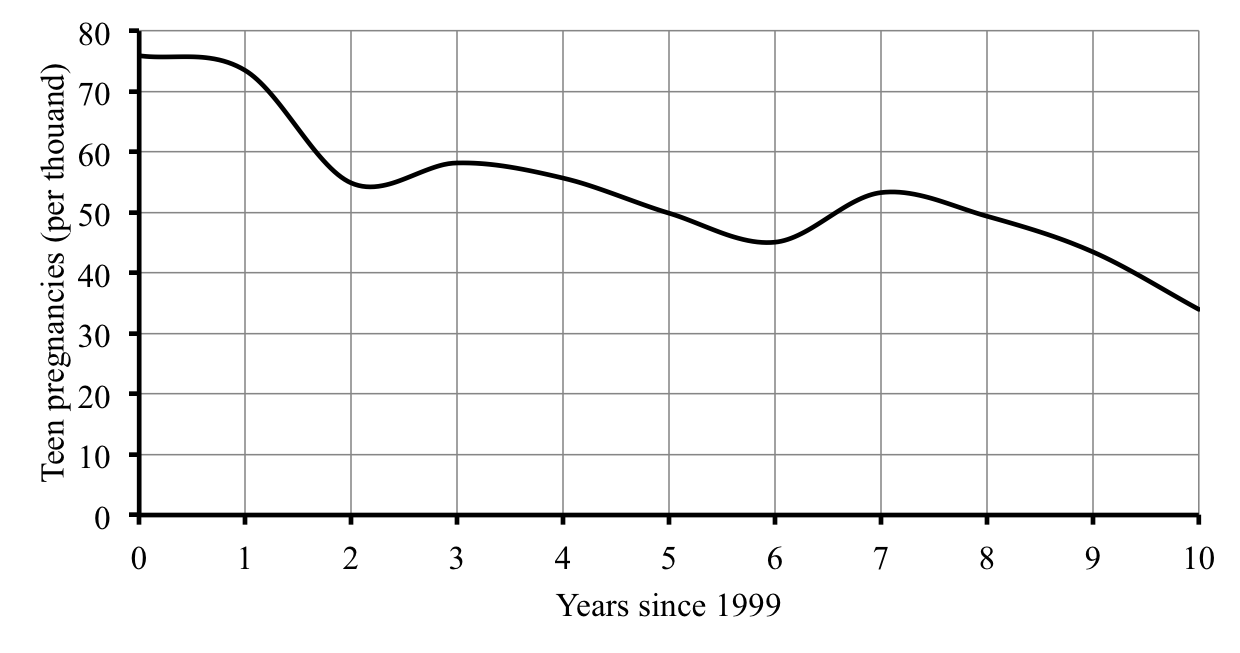
\includegraphics[width=\linewidth]{external/teenpregnancy.png}
\end{image}%
\begin{enumerate}[label=(\alph*),ref=\alph*]%
\item{}What was the teen pregnancy rate in 2003?%
\par\rule{\workspacestrutwidth}{0.45in}%
\item{}Did the teen pregnancy rate increase or decrease from 2003 to 2004?%
\par\rule{\workspacestrutwidth}{0.45in}%
\item{}While the teen pregnancy rate has generally decreased, from 2001 to 2002 it actually increased. Were there other times when it increased?%
\par\rule{\workspacestrutwidth}{0.45in}%
\item{}When did the teen pregnancy rate first fall below 60 pregnancies per thousand teens?%
\par\rule{\workspacestrutwidth}{0.45in}%
\item{}How fast was the teen pregnancy rate dropping on average per year from 2002 to 2005? How does that compare to 2006 to 2009?%
\par\rule{\workspacestrutwidth}{0.45in}%
\end{enumerate}%
\end{divisionexercise}%
\end{exercises-subsection-numberless}
\begin{conclusion}{When you're done \textellipsis{}}%
%
\begin{itemize}[label=\textbullet]
\item{}Check your solutions. Still confused? Work with a classmate, instructor, or tutor.%
\item{}Try the \alert{Do you know} questions. Not sure? Read the textbook and try again.%
\item{}Make a list of key ideas and processes to remember under \alert{Don't forget!}%
\item{}Do the textbook exercises and check your answers. Not sure if you are close enough? Compare answers with a classmate or ask your instructor or tutor.%
\item{}Getting the wrong answers or stuck? Re-read the section and try again. If you are still stuck, work with a classmate or go to your instructor's office hours or tutor hours.%
\item{}It is normal to find some parts of exercises difficult, but if most of them are a struggle, meet with your instructor or advisor about possible strategies or support services.%
\end{itemize}
%
\end{conclusion}%
\begin{conclusion}{Do you know \textellipsis{}}%
%
\begin{enumerate}[label={\Alph*.}]
\item{}How to calculate rate of change between two points? \emph{Ask your instructor if you need to remember the formula or if it will be provided during the exam.}%
\item{}What the rate of change means in the story?%
\item{}How we can use the rate of change to estimate values?%
\item{}When a function is increasing or decreasing, and the connection to the rate of change?%
\item{}Why the rate of change is zero at the maximum (or minimum) value of a function?%
\item{}What the connection is between rate of change and the steepness of the graph?%
\end{enumerate}
%
\par
\alert{Don't forget!}%
\end{conclusion}%
\end{sectionptx}
%
%
\typeout{************************************************}
\typeout{Section 1.4 Units - Practice exercises}
\typeout{************************************************}
%
\begin{sectionptx}{Section}{Units - Practice exercises}{}{Units - Practice exercises}{}{}{sec-1-4-Units}
%
%
\typeout{************************************************}
\typeout{Exercises 1.4 Exercises}
\typeout{************************************************}
%
\begin{exercises-subsection-numberless}{Exercises}{Exercises}{}{Exercises}{}{}{ex-1-4-Units}
\begin{divisionexercise}{1}{}{}{compare-lengths-units}%
\vspace{-\baselineskip-\parsep}%
\begin{enumerate}[label=(\alph*),ref=\alph*]%
\item{}Compare centimeters (cm) and inches, using that 1 inch \(\approx\) 2.54 cm.%
\begin{enumerate}[label=\roman*.,ref=\theenumi.\roman*]%
\item{}Which is longer: 1 inch or 1 centimeter?%
\par\rule{\workspacestrutwidth}{0cm}%
\item{}Kamari is shopping at an internationally-based retail store. She is looking at a curtain rod that projects 10 cm from the wall. What is that in inches?%
\par\rule{\workspacestrutwidth}{1cm}%
\item{}She also wants a basket no more than 1 foot wide or long to fit on her bookcase. How many centimeters are in a foot?%
\par\rule{\workspacestrutwidth}{1cm}%
\end{enumerate}%
\item{}Compare meters (m) and yards using that 1 yard \(\approx\) 0.9144 m.%
\begin{enumerate}[label=\roman*.,ref=\theenumi.\roman*]%
\item{}Which is longer: 1 yard or 1 meter?%
\par\rule{\workspacestrutwidth}{0cm}%
\item{}Princeton was watching the Olympics and noticed everything was measured in meters. He is curious how long a football field (100 yards) is in meters.%
\par\rule{\workspacestrutwidth}{1cm}%
\item{}Kamari found a really big bath towel she likes. It is 1 meter wide and 1.5 meters long. What are the dimensions in inches? Use that 1 yard = 3 feet.%
\par\rule{\workspacestrutwidth}{1cm}%
\end{enumerate}%
\item{}Compare kilometers (km) and miles using that 1 mile \(\approx\) 1.609 km.%
\begin{enumerate}[label=\roman*.,ref=\theenumi.\roman*]%
\item{}Which is longer: 1 mile or 1 kilometer?%
\par\rule{\workspacestrutwidth}{0cm}%
\item{}This weekend Princeton and Kamari are doing a 5K run. How many miles long is that? Note: \terminology{5K} is short for 5 kilometers.%
\par\rule{\workspacestrutwidth}{1cm}%
\item{}Princeton is actually in training for a marathon. How many kilometers is that? Note: a \terminology{marathon} is approximately 26.2 miles.%
\par\rule{\workspacestrutwidth}{0in}%
\end{enumerate}%
\end{enumerate}%
\end{divisionexercise}%
\clearpage
\begin{divisionexercise}{2}{}{}{decimal-hours-lengths-units}%
\vspace{-\baselineskip-\parsep}%
\begin{enumerate}[label=(\alph*),ref=\alph*]%
\item{}Yesterday Cameron worked for 2 hours and 15 minutes (that's 2:15) and then went home and studied for 7 hours and 57 minutes (that's 7:57). Convert each time into decimal hours.%
\par\rule{\workspacestrutwidth}{1in}%
\item{}Ephraim works at a plant that produces very delicate electronic switches. He measured the lifetime for one switch at 4.18 hours. Another had lifetime 19.50 hours. Convert each time into hours and minutes. \emph{That means H:MM format.}%
\par\rule{\workspacestrutwidth}{1in}%
\item{}Phillip measured his office using a digital measure. One wall is 21.8 feet. The other is 10.2 feet. How long is each wall measured in the more usual feet and inches?%
\par\rule{\workspacestrutwidth}{1in}%
\item{}The couch Stetson wanted to buy is 92\textquotesingle\textquotesingle{} long and 44\textquotesingle\textquotesingle{} tall. Convert the length and height to feet and inches.%
\par\rule{\workspacestrutwidth}{1in}%
\item{}Abdi volunteers at a food bank. He noticed that the shelf on the back wall was bending so he measured its length at 12\textquotesingle{}5\textquotesingle\textquotesingle{}. The formula for load needs the length written as a decimal. Convert the length to a decimal number of feet.%
\par\rule{\workspacestrutwidth}{0in}%
\end{enumerate}%
\end{divisionexercise}%
\clearpage
\begin{divisionexercise}{3}{}{}{drink-water-units}%
Some people say we should drink 8 glasses of water (or other liquids) every day, where a glass is defined as 8 (liquid) ounces.%
\begin{enumerate}[label=(\alph*),ref=\alph*]%
\item{}Ingrid uses a 20 ounce unbreakable plastic bottle. How many of those bottles full of water does she need to drink each day?%
\par\rule{\workspacestrutwidth}{2in}%
\item{}Siri carries around a insulated water bottle that holds 0.6 liters. How many of those bottles full of water does she need to drink each day? Use that 1 liter \(\approx\) 1.057 quarts and 1 quart = 32 (liquid) ounces.%
\par\rule{\workspacestrutwidth}{2in}%
\item{}To meet the recommendation, how much water would one person drink in an entire year? Give the answer in gallons. Use 1 gallon = 4 quarts.%
\end{enumerate}%
\end{divisionexercise}%
\clearpage
\begin{divisionexercise}{4}{}{}{finland-units}%
Jenna is studying in Finland this term and rented an older car to drive.%
\begin{enumerate}[label=(\alph*),ref=\alph*]%
\item{}She learns that no matter what the road signs might say, the maximum speed limit in Finland in winter is never more than 100 km\slash{}hr. How fast is that in miles per hour (mph)? Use 1 mile \(\approx\) 1.609 km.%
\par\rule{\workspacestrutwidth}{2.75cm}%
\item{}Jenna's car holds 62 liters of gasoline in its tank. How many gallons is that? Use 1 liter \(\approx\) 1.057 quarts and 1 gallon = 4 quarts.%
\par\rule{\workspacestrutwidth}{2.75cm}%
\item{}Her car gets 7.6 km\slash{}liter. Convert to miles per gallon (mpg).%
\par\rule{\workspacestrutwidth}{2.75cm}%
\item{}Gas prices in Finland were 1.658 €\slash{}liter. What's the equivalent price in \textdollar{}\slash{}gal? The symbol € stands for euro. Use 1 € \(\approx\) \textdollar{}1.23.%
\par\rule{\workspacestrutwidth}{2.75cm}%
\item{}What would it cost Jenna, in euros, for a full tank of gas? How much is that in dollars?%
\par\rule{\workspacestrutwidth}{2.75cm}%
\end{enumerate}%
\end{divisionexercise}%
\end{exercises-subsection-numberless}
\begin{conclusion}{When you're done \textellipsis{}}%
%
\begin{itemize}[label=\textbullet]
\item{}Check your solutions. Still confused? Work with a classmate, instructor, or tutor.%
\item{}Try the \alert{Do you know} questions. Not sure? Read the textbook and try again.%
\item{}Make a list of key ideas and processes to remember under \alert{Don't forget!}%
\item{}Do the textbook exercises and check your answers. Not sure if you are close enough? Compare answers with a classmate or ask your instructor or tutor.%
\item{}Getting the wrong answers or stuck? Re-read the section and try again. If you are still stuck, work with a classmate or go to your instructor's office hours or tutor hours.%
\item{}It is normal to find some parts of exercises difficult, but if most of them are a struggle, meet with your instructor or advisor about possible strategies or support services.%
\end{itemize}
%
\end{conclusion}%
\begin{conclusion}{Do you know \textellipsis{}}%
%
\begin{enumerate}[label={\Alph*.}]
\item{}How to convert from one unit of measurement to another?%
\item{}What a unit conversion fraction is?%
\item{}How to decide whether to multiply or divide?%
\item{}Why multiplying by a unit conversion fraction doesn't change the amount, just the units?%
\item{}How to connect repeated conversions into one calculation?%
\item{}Why if we convert an amount to a larger unit, we use a smaller number?%
\item{}How many seconds in a minute, minutes in an hour, hours in a day, days in a year, inches in a foot, feet in a mile, and other common conversions?%
\par
\emph{Ask your instructor which common conversions you need to remember, and whether any conversion formulas will be provided during the exam.}%
\item{}How to convert between English and metric measurements?%
\par
\emph{Again, ask your instructor which metric conversions you need to remember, and whether any conversion formulas will be provided during the exam.}%
\end{enumerate}
%
\par
\alert{Don't forget!}%
\end{conclusion}%
\end{sectionptx}
%
%
\typeout{************************************************}
\typeout{Section 1.5 Metric prefixes and scientific notation - Practice exercises}
\typeout{************************************************}
%
\begin{sectionptx}{Section}{Metric prefixes and scientific notation - Practice exercises}{}{Metric prefixes and scientific notation - Practice exercises}{}{}{sec-1-5-Metric_system_and_scientific_notation}
%
%
\typeout{************************************************}
\typeout{Exercises 1.5 Exercises}
\typeout{************************************************}
%
\begin{exercises-subsection-numberless}{Exercises}{Exercises}{}{Exercises}{}{}{ex-1-5-Metric_system_and_scientific_notation}
\begin{divisionexercise}{1}{}{}{gdp-scientific-notation}%
In 2011, \begin{aside}{Aside}{}{gdp-scientific-notation-1-1-1}%
Source: U.S. Bureau of Economic Analysis, U.S. Census Bureau%
\par
(Story also appears in \hyperref[gdp-prelude-scientific-notation]{{\xreffont 0.8.1}.{\xreffont\ref{gdp-prelude-scientific-notation}}})%
\end{aside}
 the GDP (gross domestic product) of the United States was approximately \textdollar{}15,596 billion in 2011 and the population of the United States was approximately 0.313 billion that year.%
\begin{enumerate}[label=(\alph*),ref=\alph*]%
\item{}Writing the population as 0.313 billion seems strange. A more natural unit would be millions. Rewrite the population in millions of people.%
\par\rule{\workspacestrutwidth}{1.5cm}%
\item{}Rewrite the population in people, both in normal decimal notation (that means with all the 0s) and in scientific notation.%
\par\rule{\workspacestrutwidth}{1.5cm}%
\item{}It also seems strange to write the GDP as \textdollar{}15,596 billion. A more natural unit would be \terminology{trillions}, where 1 trillion = 1,000,000,000,000. Rewrite the GDP in trillions of dollars.%
\par\rule{\workspacestrutwidth}{1.5cm}%
\item{}Rewrite the GDP in dollars, both in normal decimal notation and in scientific notation.%
\par\rule{\workspacestrutwidth}{1.5cm}%
\item{}Calculate the GDP \terminology{per capita} (meaning per person) by dividing the GDP in dollars by the population in people. Express your answer in \textdollar{}\slash{}person.%
\par\rule{\workspacestrutwidth}{1.5cm}%
\item{}For practice, repeat your calculation using the numbers in scientific notation.%
\par
\emph{Because \(\times\) and \(\div\) are at the same level in the order of operations, you need to put parentheses around each number in scientific notation before dividing.}%
\par\rule{\workspacestrutwidth}{1.5cm}%
\end{enumerate}%
\end{divisionexercise}%
\clearpage
\begin{divisionexercise}{2}{}{}{dust-particle-scientific-notation}%
Edgar recently changed the cleaning bag on his vacuum cleaner. \begin{aside}{Aside}{}{dust-particle-scientific-notation-1-1-1}%
(Story also appears in \hyperref[dust-particle-prelude-scientific-notation]{{\xreffont 0.8.2}.{\xreffont\ref{dust-particle-prelude-scientific-notation}}})%
\end{aside}
 He became curious about how many particles of dust were in the bag. Edgar did a little research online and found out that the mass of a dust particle is%
\begin{equation*}
0.000~000~000~753\text{ kilograms.}
\end{equation*}
(The strange-looking spaces are to help you see that there are 9 zeros in the number.)%
\begin{enumerate}[label=(\alph*),ref=\alph*]%
\item{}Write the mass of a dust particle in scientific notation.%
\par\rule{\workspacestrutwidth}{1cm}%
\item{}Recall that%
\begin{align*}
\amp\textbf{kilo} \amp
\amp= \amp 
\amp 1 \text{ thousand} \amp
\amp =\amp
1{,}000\amp\amp
\amp=\amp
10^3\amp\\
\amp\textbf{milli} \amp
\amp= \amp 
\amp 1 \text{ in a thousand} \amp
\amp =\amp
0\amp.001\amp
\amp=\amp
10^{-3}\amp\\
\amp\textbf{micro} \amp
\amp= \amp 
\amp 1 \text{ in a million} \amp
\amp =\amp
0\amp.000~001\amp
\amp=\amp
10^{-6}\amp\\
\amp\textbf{nano} \amp
\amp= \amp 
\amp 1 \text{ in a billion} \amp
\amp =\amp
0\amp.000~000~001\amp
\amp=\amp
10^{-9}\amp
\end{align*}
Express the mass of a dust particle in each of the given units:%
\begin{enumerate}[label=\roman*.,ref=\theenumi.\roman*]%
\item{}grams%
\par\rule{\workspacestrutwidth}{1cm}%
\item{}milligrams (mg)%
\par\rule{\workspacestrutwidth}{1cm}%
\item{}micrograms (\(\mu\)g)%
\par\rule{\workspacestrutwidth}{1cm}%
\item{}nanograms (ng)%
\par\rule{\workspacestrutwidth}{1cm}%
\end{enumerate}%
\item{}Edgar determined that the full vacuum bag weighed 5 pounds. How many dust particles were in the bag? (I am already sneezing.) Use \(1 \text{ kilogram} \approx 2.2 \text{ pounds}\). Express your answer in scientific notation.%
\par\rule{\workspacestrutwidth}{1cm}%
\end{enumerate}%
\end{divisionexercise}%
\clearpage
\begin{divisionexercise}{3}{}{}{planet-weight-scientific-notation}%
The list shows the (approximate) mass of the planets in our solar system. \begin{aside}{Aside}{}{planet-weight-scientific-notation-1-1-1}%
Source: Wikipedia (Solar System)%
\par
(Story also appears in \hyperref[earth-weight-prelude-scientific-notation]{{\xreffont 0.8.1}.{\xreffont\ref{earth-weight-prelude-scientific-notation}}})%
\end{aside}
%
 \begin{center}%
{\tabularfont%
\begin{tabular}{ll}
Earth&\(5.972 \times 10^{24}\) kg\tabularnewline[0pt]
Jupiter&\(1.899 \times 10^{27}\) kg\tabularnewline[0pt]
Mars&\(6.417 \times 10^{23}\) kg\tabularnewline[0pt]
Mercury&\(3.302 \times 10^{23}\) kg\tabularnewline[0pt]
Neptune&\(1.024 \times 10^{26}\) kg\tabularnewline[0pt]
Saturn&\(5.685 \times 10^{26}\) kg\tabularnewline[0pt]
Uranus&\(8.681 \times 10^{25}\) kg\tabularnewline[0pt]
Venus&\(4.868 \times 10^{24}\) kg
\end{tabular}
}%
\end{center}%
\begin{enumerate}[label=(\alph*),ref=\alph*]%
\item{}Write the mass of Earth and the mass of Mars in standard decimal notation. Which is heavier?%
\par\rule{\workspacestrutwidth}{1.25in}%
\item{}List the planets from heaviest (largest mass) to lightest (smallest mass).%
\par\rule{\workspacestrutwidth}{1.25in}%
\item{}The mass of astronomical bodies are sometimes measured in \terminology{Jupiter mass}, abbreviated \(M_J\), where \(1 M_J = 1.899 \times 10^{27}\) kg. Express Earth's mass in \(M_J\).%
\par
\emph{Because \(\times\) and \(\div\) are at the same level in the order of operations, you need to put parentheses around each number in scientific notation before dividing.}%
\par\rule{\workspacestrutwidth}{1.25in}%
\end{enumerate}%
\end{divisionexercise}%
\clearpage
\begin{divisionexercise}{4}{}{}{iv-drip-scientific-notation}%
Souksavanh is setting up a patient's intravenous (IV) medication. \begin{aside}{Aside}{}{iv-drip-scientific-notation-1-1-1}%
(Story also appears in \hyperref[sec-0-1-Approximation_and_rounding]{{\xreffont\ref{sec-0-1-Approximation_and_rounding}}} Exercises)%
\end{aside}
 She sets the drip at 42 drops\slash{}minute. The drip chamber size is 20 drops\slash{}mL. Recall%
\begin{align*}
\amp\textbf{milli} \amp
\amp= \amp 
\amp 1 \text{ in a thousand} \amp
\amp =\amp
0\amp.001\amp
\amp=\amp
10^{-3}\amp\\
\amp\textbf{micro} \amp
\amp= \amp 
\amp 1 \text{ in a million} \amp
\amp =\amp
0\amp.000~001\amp
\amp=\amp
10^{-6}\amp
\end{align*}
%
\begin{enumerate}[label=(\alph*),ref=\alph*]%
\item{}At what rate is the IV fluid being delivered to Souk's patient? Answer in mL\slash{}min (millileters per minute).%
\par\rule{\workspacestrutwidth}{2.25cm}%
\item{}How fast is the drip measured in \(\mu\)L\slash{}sec (microliters per second)?%
\par\rule{\workspacestrutwidth}{2.25cm}%
\item{}If the drip bag holds 1 liter, how long will it take the drip to run? Express your answer in hours and minutes.%
\par\rule{\workspacestrutwidth}{2.25cm}%
\item{}The concentration of medication is 1.7 mg\slash{}mL (milligrams per milliliter). How much medication is in the 1 liter bag? Convert your answer to grams. Explain what you notice.%
\par\rule{\workspacestrutwidth}{2.25cm}%
\item{}At what rate is the medication being delivered to Souk's patient? Answer in g\slash{}min (grams per minute).%
\par\rule{\workspacestrutwidth}{2.25cm}%
\end{enumerate}%
\end{divisionexercise}%
\end{exercises-subsection-numberless}
\begin{conclusion}{When you're done \textellipsis{}}%
%
\begin{itemize}[label=\textbullet]
\item{}Check your solutions. Still confused? Work with a classmate, instructor, or tutor.%
\item{}Try the \alert{Do you know} questions. Not sure? Read the textbook and try again.%
\item{}Make a list of key ideas and processes to remember under \alert{Don't forget!}%
\item{}Do the textbook exercises and check your answers. Not sure if you are close enough? Compare answers with a classmate or ask your instructor or tutor.%
\item{}Getting the wrong answers or stuck? Re-read the section and try again. If you are still stuck, work with a classmate or go to your instructor's office hours or tutor hours.%
\item{}It is normal to find some parts of exercises difficult, but if most of them are a struggle, meet with your instructor or advisor about possible strategies or support services.%
\end{itemize}
%
\end{conclusion}%
\begin{conclusion}{Do you know \textellipsis{}}%
%
\begin{enumerate}[label={\Alph*.}]
\item{}How to calculate powers on your calculator?%
\item{}What million, billion, and trillion mean?%
\item{}Why metric prefixes are used?%
\item{}What common metric prefixes (mega, giga, kilo, centi, milli, micro, nano) mean?%
\par
\emph{Ask your instructor which prefixes you need to remember, and whether any prefixes will be provided during the exam.}%
\item{}Why scientific notation is used?%
\item{}The standard format for scientific notation?%
\item{}What kinds of numbers have a positive order of magnitude, and which have a negative order of magnitude?%
\item{}How to convert between decimal notation and scientific notation?%
\item{}How your calculator reports numbers in scientific notation, and what (might be) different when you're reporting that number?%
\item{}The usual order of operations (PEMDAS) and how to use parentheses when you want a different order?%
\end{enumerate}
%
\par
\alert{Don't forget!}%
\end{conclusion}%
\end{sectionptx}
%
%
\typeout{************************************************}
\typeout{Section 1.6 Practice Exam 1A}
\typeout{************************************************}
%
\begin{sectionptx}{Section}{Practice Exam 1A}{}{Practice Exam 1A}{}{}{sec-PE1A}
%
%
\typeout{************************************************}
\typeout{Exercises 1.6 Exercises}
\typeout{************************************************}
%
\begin{exercises-subsection-numberless}{Exercises}{Exercises}{}{Exercises}{}{}{ws-PE1A}
\begin{introduction}{}%
Relax. You have done problems like these before. Even if these problems look a bit different, just do what you can. If you're not sure of something, please ask! You may use your calculator. Please show all of your work and write down as many steps as you can. Don't spend too much time on any one problem. Do well. And remember, ask me if you're not sure about something.%
\par
\emph{As you work, make a ``don't forget'' list of any information you need to look up or ask about.}%
\end{introduction}%
\begin{divisionexercise}{1}{}{}{hiking-PE1A}%
Arva and Ellie began hiking at an elevation of 1,500 feet and climbed at the steady rate of 600 vertical feet per hour.%
\begin{enumerate}[label=(\alph*),ref=\alph*]%
\item{}Name the variables, including units.%
\par\rule{\workspacestrutwidth}{1in}%
\item{}Explain the dependence using a sentence of the form ``\fillintext{3} is a function of \fillintext{3}.''%
\par\rule{\workspacestrutwidth}{0.5in}%
\item{}Make a table showing their elevation after 1 hour, 2 hours, and 5 hours.%
\par\rule{\workspacestrutwidth}{1in}%
\item{}Is the function increasing or decreasing?%
\par\rule{\workspacestrutwidth}{0.5in}%
\item{}How long does it take them to reach 5,300 feet up? Try to figure out the answer in hours and minutes (H:MM format).%
\par\rule{\workspacestrutwidth}{1in}%
\end{enumerate}%
\end{divisionexercise}%
\clearpage
\begin{divisionexercise}{2}{}{}{baby-weight-PE1A}%
The table shows Henry's weight as a baby.%
 \begin{center}%
{\tabularfont%
\begin{tabular}{llll}\hrulethin
\multicolumn{1}{AlA}{Age (weeks)}&\multicolumn{1}{cA}{0}&\multicolumn{1}{cA}{12}&\multicolumn{1}{cA}{15}\tabularnewline\hrulethin
\multicolumn{1}{AlA}{Weight (pounds)}&\multicolumn{1}{cA}{8}&\multicolumn{1}{cA}{14}&\multicolumn{1}{cA}{16}\tabularnewline\hrulethin
\end{tabular}
}%
\end{center}%
\begin{enumerate}[label=(\alph*),ref=\alph*]%
\item{}Identify the variables, including units and dependence.%
\par\rule{\workspacestrutwidth}{0.5in}%
\item{}How much weight did Henry gain, on average, each week during his first 12 weeks?%
\par\rule{\workspacestrutwidth}{0.5in}%
\item{}During which time interval was Henry gaining weight faster? \emph{Explain.}%
\par\rule{\workspacestrutwidth}{0.5in}%
\item{}Draw a graph illustrating the dependence. Choose a scale that shows up to 20 weeks and 20 pounds.%
\begin{image}{0.05}{0.9}{0.05}{}%

\includegraphics[width=\linewidth]{external/GraphPaper.jpg}
\end{image}%
\par\rule{\workspacestrutwidth}{0in}%
\item{}What might you guess for Henry's weight at 20 weeks?%
\par\rule{\workspacestrutwidth}{0.5in}%
\end{enumerate}%
\end{divisionexercise}%
\clearpage
\begin{divisionexercise}{3}{}{}{gas-PE1A}%
Pramesh's new car used 20.5 gallons of gas for a 715 mile trip.%
\begin{enumerate}[label=(\alph*),ref=\alph*]%
\item{}How many miles per gallon (mpg) does his car get?%
\par\rule{\workspacestrutwidth}{2in}%
\item{}At that rate, how many gallons of gas would Pramesh use on his 3,200 mile cross-country trip?%
\par\rule{\workspacestrutwidth}{2in}%
\item{}If gas costs \textdollar{}3.799\slash{}gallon, how much will gas for that trip cost?%
\par\rule{\workspacestrutwidth}{2in}%
\end{enumerate}%
\end{divisionexercise}%
\clearpage
\begin{divisionexercise}{4}{}{}{atoms-PE1A}%
Ndwiga is reading an article in the paper about atoms. From his physics textbook he discovered that the size of an atom is 0.142 nanometers.%
\begin{enumerate}[label=(\alph*),ref=\alph*]%
\item{}Write the size of an atom in meters. Use 1 meter = 1,000,000,000 nanometers. Write your answer in usual decimal notation and in scientific notation.%
\par\rule{\workspacestrutwidth}{3in}%
\item{}Ndwiga would like to know how many atoms across this sheet of paper which is 8.5 inches wide. Use that \(1 \text{ inch} \approx 2.54 \text{ cm}\) and \(1 \text{ meter} = 100 \text{ cm}\). Express your final answer in billions of atoms.%
\par\rule{\workspacestrutwidth}{3in}%
\end{enumerate}%
\end{divisionexercise}%
\end{exercises-subsection-numberless}
\end{sectionptx}
%
%
\typeout{************************************************}
\typeout{Section 1.7 Practice Exam 1B}
\typeout{************************************************}
%
\begin{sectionptx}{Section}{Practice Exam 1B}{}{Practice Exam 1B}{}{}{sec-PE1B}
%
%
\typeout{************************************************}
\typeout{Exercises 1.7 Practice Exam 1B}
\typeout{************************************************}
%
\begin{exercises-subsection-numberless}{Exercises}{Practice Exam 1B}{}{Practice Exam 1B}{}{}{ws-PE1B}
\begin{introduction}{}%
\emph{Try taking this version of the practice exam under testing conditions: no book, no notes, no classmate's help, no electronics (computer, cell phone, television). Give yourself one hour to work and wait until you have tried your best on all of the problems before checking any answers.}%
\end{introduction}%
\begin{divisionexercise}{1}{}{}{nursing-costs-PE1B}%
The amount of money spent on nursing home care for seniors has continued to rise. The table shows the values for select years. Here \(S\) is the spending, measured in billions of dollars, and \(T\) is time, measured in years since 1960.%
 \begin{center}%
{\tabularfont%
\begin{tabular}{llllll}\hrulethin
\multicolumn{1}{AcA}{\(T\)}&\multicolumn{1}{cA}{0}&\multicolumn{1}{cA}{10}&\multicolumn{1}{cA}{25}&\multicolumn{1}{cA}{40}&\multicolumn{1}{cA}{52}\tabularnewline\hrulethin
\multicolumn{1}{AcA}{\(S\)}&\multicolumn{1}{cA}{1.0}&\multicolumn{1}{cA}{3.3}&\multicolumn{1}{cA}{33.7}&\multicolumn{1}{cA}{96.6}&\multicolumn{1}{cA}{170.3}\tabularnewline\hrulethin
\end{tabular}
}%
\end{center}%
\begin{enumerate}[label=(\alph*),ref=\alph*]%
\item{}According to the table, what was the spending in 1970?%
\par\rule{\workspacestrutwidth}{1in}%
\item{}According to the table, what was the spending in 1985?%
\par\rule{\workspacestrutwidth}{1in}%
\item{}Calculate the rate of change of spending over the period 1970 to 1985. Don't forget to state the units.%
\par\rule{\workspacestrutwidth}{1.5in}%
\item{}In approximately what year did spending first pass \textdollar{}50 billion?%
\par\rule{\workspacestrutwidth}{0.75in}%
\end{enumerate}%
\end{divisionexercise}%
\clearpage
\begin{divisionexercise}{2}{}{}{swimming-pool-PE1B}%
Trish is filling a swimming pool with water. The graph below shows how many gallons of water (\(G\)) are in the pool after \(H\) hours. Use the graph to answer the following questions.%
 \begin{image}{0}{1}{0}{}%
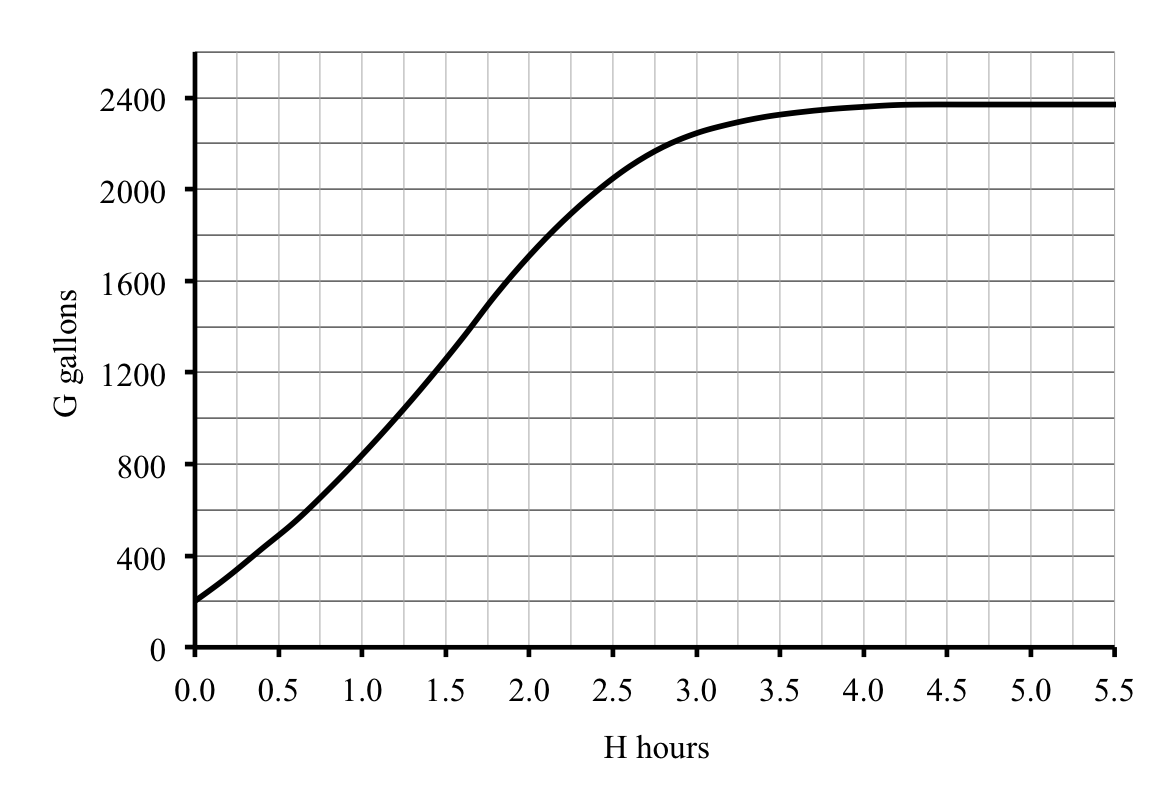
\includegraphics[width=\linewidth]{external/fillingtankNEW.png}
\end{image}%
\begin{enumerate}[label=(\alph*),ref=\alph*]%
\item{}How much water was in the swimming pool already when Trish began?%
\par\rule{\workspacestrutwidth}{0.7cm}%
\item{}How much water was in the swimming pool after 3 hours?%
\par\rule{\workspacestrutwidth}{0.7cm}%
\item{}After how many hours were there 1,000 gallons of water in the swimming pool?%
\par\rule{\workspacestrutwidth}{0.7cm}%
\item{}Was Trish filling the pool faster at 2 hours or at 2.5 hours? Explain how you see that on the graph.%
\par\rule{\workspacestrutwidth}{0.7cm}%
\item{}After (about) how many hours did Trish stop filling the swimming pool? Explain how you see that on the graph.%
\par\rule{\workspacestrutwidth}{0.7cm}%
\end{enumerate}%
\end{divisionexercise}%
\clearpage
\begin{divisionexercise}{3}{}{}{property-tax-PE1B}%
In 1990 the Lefèvre's property tax was \textdollar{}450, but it doubled every year thereafter.%
\begin{enumerate}[label=(\alph*),ref=\alph*]%
\item{}Name the variables, including units.%
\par\rule{\workspacestrutwidth}{1.4in}%
\item{}Which is the independent variable and which is the dependent variable?%
\par\rule{\workspacestrutwidth}{0.5in}%
\item{}Make a table showing the property tax each year from 1990 to 1994.%
\par\rule{\workspacestrutwidth}{1.4in}%
\item{}Draw a graph illustrating the dependence.%
\begin{image}{0.05}{0.9}{0.05}{}%

\includegraphics[width=\linewidth]{external/GraphPaper.jpg}
\end{image}%
\par\rule{\workspacestrutwidth}{0in}%
\end{enumerate}%
\end{divisionexercise}%
\clearpage
\begin{divisionexercise}{4}{}{}{earth-moon-PE1B}%
The distance from the Earth to the Moon is approximately 384,000,000 meters. \begin{aside}{Aside}{}{earth-moon-PE1B-1-1-1}%
Source: Wikipedia (Lunar distance)%
\end{aside}
%
\begin{enumerate}[label=(\alph*),ref=\alph*]%
\item{}Express this distance using scientific notation.%
\par\rule{\workspacestrutwidth}{1in}%
\item{}Express this distance in kilometers (km), using 1 km = 1,000 meters.%
\par\rule{\workspacestrutwidth}{1.5in}%
\item{}Express this distance in miles, using \(1 \text{ mile} \approx 1.609 \text{ km}\).%
\par\rule{\workspacestrutwidth}{1.5in}%
\item{}If you could drive to the moon at 55 mph, how long would it take to get there? Express your answer in terms of months, using \(1 \text{ month} \approx 30 \text{ days}\).%
\par\rule{\workspacestrutwidth}{0in}%
\end{enumerate}%
\end{divisionexercise}%
\end{exercises-subsection-numberless}
\end{sectionptx}
\end{chapterptx}
%
%
\typeout{************************************************}
\typeout{Chapter 2 Equations}
\typeout{************************************************}
%
\begin{chapterptx}{Chapter}{Equations}{}{Equations}{}{}{ch-2-Equations}
\renewcommand*{\chaptername}{Chapter}
%
%
\typeout{************************************************}
\typeout{Section 2.1 A first look at linear equations - Practice exercises}
\typeout{************************************************}
%
\begin{sectionptx}{Section}{A first look at linear equations - Practice exercises}{}{A first look at linear equations - Practice exercises}{}{}{sec-2-1-First_look_linear}
%
%
\typeout{************************************************}
\typeout{Exercises 2.1 Exercises}
\typeout{************************************************}
%
\begin{exercises-subsection-numberless}{Exercises}{Exercises}{}{Exercises}{}{}{ex-2-1-First_look_linear}
\begin{divisionexercise}{1}{}{}{truck-grass-first-look-linear}%
A truck hauling bags of grass seed pulls into a weigh station along the highway. \begin{aside}{Aside}{}{truck-grass-first-look-linear-1-1-1}%
(Story also appears in \hyperlink{truck-grass-arithmetic-operations}{{\xreffont 0.2.4}}, \hyperlink{truck-grass-solving-linear}{{\xreffont 3.1.1}}, and \hyperlink{truck-grass-linear-ineq}{{\xreffont 3.2.1}})%
\end{aside}
 Trucks are weighed to determine the amount of highway tax. This particular truck weighs 3,900 pounds when it is empty. Each bag of grass seed it carries weighs 4.2 pounds. For example, a truck carrying 1,000 bags of grass seed weighs%
\begin{equation*}
3{,}900 \text{ pounds} + \frac{4.2 \text{ pounds}}{\text{bag}} \ast 1{,}000 \text{  bags} 
= 3{,}900 + 4.2\times 1{,}000
= 8{,}100 \text{ pounds}
\end{equation*}
In official trucking lingo, we say the \terminology{curb weight} of pounds plus the \terminology{load weight} of pounds results in a \terminology{gross weight} of pounds. So, now you know.%
\begin{enumerate}[label=(\alph*),ref=\alph*]%
\item{}Name the variables, including units and dependence.%
\par
    \hspace{-2cm}
\begin{tikzpicture}
    \matrix (v) 
        [matrix of nodes,
        nodes={
            align=center,
            font=\bfseries
        },
        minimum height=3.5em,
        minimum width=2em,
        text depth=1ex,
        text height=2ex,
        nodes in empty cells,
        row 1/.style={minimum height=1.5em},
        column 3/.style={text width=0.6\linewidth},
        column 6/.style={text width=5em}
        ]
    {
        letter\amp =\amp everyday words\amp (units)\amp {\huge\textasciitilde} \amp 
        |[text depth = 1.5em, anchor=center]| dep or indep\\
        \phantom{letter}\amp=\amp\amp\Bigg(\phantom{units}\Bigg)\amp{\huge\textasciitilde}\amp\\
        \phantom{letter}\amp=\amp\amp\Bigg(\phantom{units}\Bigg)\amp{\huge\textasciitilde}\amp\\
    };
    \draw[black] (v-1-1.north west) rectangle (v-1-6.south east);
    \draw[black] (v-2-1.north west) rectangle (v-2-6.south east);
    \draw[black] (v-3-1.north west) rectangle (v-3-6.south east);
\end{tikzpicture}%
%
\item{}Calculate the gross weight of the truck if it contains 2,000 bags of grass seed.%
\par\rule{\workspacestrutwidth}{0.75in}%
\item{}Write an equation showing how the gross weight of the truck is a function of the number of bags of grass seed.%
\par\rule{\workspacestrutwidth}{0.75in}%
\item{}Identify the slope and intercept, along with their units. Explain what each means in terms of the story.%
\par\rule{\workspacestrutwidth}{0.75in}%
\item{}The bags of grass seed are piled on wood \terminology{pallets} (sturdy platforms) to make them more stable for moving. How much does the truck weigh if it is carrying 12 pallets, where each pallet weighs 15 pounds and holds 96 bags of grass seed?%
\par\rule{\workspacestrutwidth}{0.25in}%
\end{enumerate}%
\end{divisionexercise}%
\clearpage
\begin{divisionexercise}{2}{}{}{reservoir-rain-first-look-linear}%
The water in the local reservoir was 47 feet deep, \begin{aside}{Aside}{}{reservoir-rain-first-look-linear-1-1-1}%
(Story also appears in \hyperref[sec-3-2-Solving_linear_inequalities]{{\xreffont\ref{sec-3-2-Solving_linear_inequalities}}} Exercises and \hyperref[reservoir-rain-modeling-linear]{{\xreffont 4.1.3}.{\xreffont\ref{reservoir-rain-modeling-linear}}})%
\end{aside}
 but there has been so little rain that the water level has dropped 18 inches a week over the past few months. Officials are worried that if dry conditions continue, the reservoir will not have enough water to supply the town.%
\begin{enumerate}[label=(\alph*),ref=\alph*]%
\item{}Name the variables and write an equation relating them. (\emph{Hint: How many feet is 18 inches?})%
\par
    \hspace{-2cm}
\begin{tikzpicture}
    \matrix (v) 
        [matrix of nodes,
        nodes={
            align=center,
            font=\bfseries
        },
        minimum height=3.5em,
        minimum width=2em,
        text depth=1ex,
        text height=2ex,
        nodes in empty cells,
        row 1/.style={minimum height=1.5em},
        column 3/.style={text width=0.6\linewidth},
        column 6/.style={text width=5em}
        ]
    {
        letter\amp =\amp everyday words\amp (units)\amp {\huge\textasciitilde} \amp 
        |[text depth = 1.5em, anchor=center]| dep or indep\\
        \phantom{letter}\amp=\amp\amp\Bigg(\phantom{units}\Bigg)\amp{\huge\textasciitilde}\amp\\
        \phantom{letter}\amp=\amp\amp\Bigg(\phantom{units}\Bigg)\amp{\huge\textasciitilde}\amp\\
    };
    \draw[black] (v-1-1.north west) rectangle (v-1-6.south east);
    \draw[black] (v-2-1.north west) rectangle (v-2-6.south east);
    \draw[black] (v-3-1.north west) rectangle (v-3-6.south east);
\end{tikzpicture}%
%
\par\rule{\workspacestrutwidth}{0.5in}%
\item{}Identify the slope and intercept, along with their units. Explain what each means in terms of the story.%
\par\rule{\workspacestrutwidth}{0.5in}%
\item{}Make a table of values showing the projected depth of the reservoir after 1 week, 5 weeks, 10 weeks, and 20 weeks if the current trend continues.%
\par\rule{\workspacestrutwidth}{0.5in}%
\item{}Draw a graph illustrating the function.%
\begin{image}{0.05}{0.9}{0.05}{}%

\includegraphics[width=\linewidth]{external/GraphPaper.jpg}
\end{image}%
\end{enumerate}%
\end{divisionexercise}%
\clearpage
\begin{divisionexercise}{3}{}{}{credit-line-first-look-linear}%
\begin{aside}{Aside}{}{credit-line-first-look-linear-1-1-1}%
(Story also appears in \hyperref[sec-3-2-Solving_linear_inequalities]{{\xreffont\ref{sec-3-2-Solving_linear_inequalities}}} Exercises)%
\end{aside}
 I was short on cash so I got a \terminology{line of credit} (short term loan) on my bank account, of which I spent \textdollar{}2,189.57. That means my account balance is \(-\$2{,}189.57\). I will pay back the interest plus an extra \textdollar{}250 each month. When the loan is paid off, I plan to continue to deposit \textdollar{}250 per month to start saving.%
\begin{enumerate}[label=(\alph*),ref=\alph*]%
\item{}Name the variables, including units and dependence. Write an equation showing my account balance in each number of months. Ignore the interest.%
\par
    \hspace{-2cm}
\begin{tikzpicture}
    \matrix (v) 
        [matrix of nodes,
        nodes={
            align=center,
            font=\bfseries
        },
        minimum height=3.5em,
        minimum width=2em,
        text depth=1ex,
        text height=2ex,
        nodes in empty cells,
        row 1/.style={minimum height=1.5em},
        column 3/.style={text width=0.6\linewidth},
        column 6/.style={text width=5em}
        ]
    {
        letter\amp =\amp everyday words\amp (units)\amp {\huge\textasciitilde} \amp 
        |[text depth = 1.5em, anchor=center]| dep or indep\\
        \phantom{letter}\amp=\amp\amp\Bigg(\phantom{units}\Bigg)\amp{\huge\textasciitilde}\amp\\
        \phantom{letter}\amp=\amp\amp\Bigg(\phantom{units}\Bigg)\amp{\huge\textasciitilde}\amp\\
    };
    \draw[black] (v-1-1.north west) rectangle (v-1-6.south east);
    \draw[black] (v-2-1.north west) rectangle (v-2-6.south east);
    \draw[black] (v-3-1.north west) rectangle (v-3-6.south east);
\end{tikzpicture}%
%
\par\rule{\workspacestrutwidth}{0.75cm}%
\item{}Identify the slope and intercept, along with their units. Explain what each means in terms of the story.%
\par\rule{\workspacestrutwidth}{0.75cm}%
\item{}Make a table of values showing my account balance now, after 4 months, after 6 months, and at the end of a year.%
\par\rule{\workspacestrutwidth}{0.75cm}%
\item{}Draw a graph showing my account balance over this coming year.%
\begin{image}{0.05}{0.9}{0.05}{}%

\includegraphics[width=\linewidth]{external/GraphPaper.jpg}
\end{image}%
\item{}\emph{About} how many months will it take to pay off my line of credit? Give an \emph{approximate} answer from the graph.%
\end{enumerate}%
\end{divisionexercise}%
\clearpage
\begin{divisionexercise}{4}{}{}{juan-coffee-first-look-linear}%
A mug of coffee costs \textdollar{}3.45 at Juan's favorite cafe, \begin{aside}{Aside}{}{juan-coffee-first-look-linear-1-1-1}%
(Story also appears in \hyperlink{juan-coffee-order-operations}{{\xreffont 0.4.1}}, \hyperlink{juan-coffee-tables-graphs}{{\xreffont 1.2.4}}, and \hyperlink{juan-coffee-systems-linear}{{\xreffont 4.2.2}})%
\end{aside}
 unless he buys their discount card for \textdollar{}10, in which case each mug costs \textdollar{}2.90.%
\begin{enumerate}[label=(\alph*),ref=\alph*]%
\item{}Name the variables, including units.%
\par
    \hspace{-2cm}
\begin{tikzpicture}
    \matrix (v) 
        [matrix of nodes,
        nodes={
            align=center,
            font=\bfseries
        },
        minimum height=3.5em,
        minimum width=2em,
        text depth=1ex,
        text height=2ex,
        nodes in empty cells,
        row 1/.style={minimum height=1.5em},
        column 3/.style={text width=0.6\linewidth},
        column 6/.style={text width=5em}
        ]
    {
        letter\amp =\amp everyday words\amp (units)\amp {\huge\textasciitilde} \amp 
        |[text depth = 1.5em, anchor=center]| dep or indep\\
        \phantom{letter}\amp=\amp\amp\Bigg(\phantom{units}\Bigg)\amp{\huge\textasciitilde}\amp\\
        \phantom{letter}\amp=\amp\amp\Bigg(\phantom{units}\Bigg)\amp{\huge\textasciitilde}\amp\\
    };
    \draw[black] (v-1-1.north west) rectangle (v-1-6.south east);
    \draw[black] (v-2-1.north west) rectangle (v-2-6.south east);
    \draw[black] (v-3-1.north west) rectangle (v-3-6.south east);
\end{tikzpicture}%
%
\par\rule{\workspacestrutwidth}{0.75in}%
\item{}Write an equation describing how the total cost depends on how many mugs of coffee Juan buys, assuming he does not buy the discount card.%
\par\rule{\workspacestrutwidth}{1.5in}%
\item{}Write an equation describing how the total cost depends on how many mugs of coffee Juan buys, if he buys the discount card.%
\par\rule{\workspacestrutwidth}{1.5in}%
\item{}How would the equation change if the cafe offers a new annual membership card that costs \textdollar{}59.99 that entitles Juan to buy coffee for only \textdollar{}1 per mug all year?%
\par\rule{\workspacestrutwidth}{1in}%
\end{enumerate}%
\end{divisionexercise}%
\end{exercises-subsection-numberless}
\begin{conclusion}{When you're done \textellipsis{}}%
%
\begin{itemize}[label=\textbullet]
\item{}Check your solutions. Still confused? Work with a classmate, instructor, or tutor.%
\item{}Try the \alert{Do you know} questions. Not sure? Read the textbook and try again.%
\item{}Make a list of key ideas and processes to remember under \alert{Don't forget!}%
\item{}Do the textbook exercises and check your answers. Not sure if you are close enough? Compare answers with a classmate or ask your instructor or tutor.%
\item{}Getting the wrong answers or stuck? Re-read the section and try again. If you are still stuck, work with a classmate or go to your instructor's office hours or tutor hours.%
\item{}It is normal to find some parts of exercises difficult, but if most of them are a struggle, meet with your instructor or advisor about possible strategies or support services.%
\end{itemize}
%
\end{conclusion}%
\begin{conclusion}{Do you know \textellipsis{}}%
%
\begin{enumerate}[label={\Alph*.}]
\item{}How to generalize from an example to find an equation?%
\item{}Where the dependent variable usually is in an equation?%
\item{}What the slope of a linear function means in the story and what it tells us about the graph?%
\item{}What the intercept of a linear function means in the story and what it tells us about the graph?%
\item{}The template for a linear equation? \emph{Ask your instructor if you need to remember the template or if it will be provided during the exam.}%
\item{}Where the slope and intercept appear in the template for a linear equation?%
\item{}What makes a function linear?%
\item{}How to plot negative numbers on a graph?%
\item{}What the graph of a linear function looks like?%
\end{enumerate}
%
\par
\alert{Don't forget!}%
\end{conclusion}%
\end{sectionptx}
%
%
\typeout{************************************************}
\typeout{Section 2.2 A first look at exponential equations - Practice exercises}
\typeout{************************************************}
%
\begin{sectionptx}{Section}{A first look at exponential equations - Practice exercises}{}{A first look at exponential equations - Practice exercises}{}{}{sec-2-2-First_look_exponential}
%
%
\typeout{************************************************}
\typeout{Exercises 2.2 Exercises}
\typeout{************************************************}
%
\begin{exercises-subsection-numberless}{Exercises}{Exercises}{}{Exercises}{}{}{ex-2-2-First_look_exponentialEX}
\begin{divisionexercise}{1}{}{}{private-college-first-look-exponential}%
The comprehensive fee at a local private college is \textdollar{}64,000. The fee is projected to increase 5.8\% per year.%
\begin{enumerate}[label=(\alph*),ref=\alph*]%
\item{}Calculate the annual growth factor.%
\par\rule{\workspacestrutwidth}{0.5cm}%
\item{}What do you expect the comprehensive fee will be in five years?%
\par\rule{\workspacestrutwidth}{0.5cm}%
\item{}Name the variables, including units, and write an equation.%
\par
    \hspace{-2cm}
\begin{tikzpicture}
    \matrix (v) 
        [matrix of nodes,
        nodes={
            align=center,
            font=\bfseries
        },
        minimum height=3.5em,
        minimum width=2em,
        text depth=1ex,
        text height=2ex,
        nodes in empty cells,
        row 1/.style={minimum height=1.5em},
        column 3/.style={text width=0.6\linewidth},
        column 6/.style={text width=5em}
        ]
    {
        letter\amp =\amp everyday words\amp (units)\amp {\huge\textasciitilde} \amp 
        |[text depth = 1.5em, anchor=center]| dep or indep\\
        \phantom{letter}\amp=\amp\amp\Bigg(\phantom{units}\Bigg)\amp{\huge\textasciitilde}\amp\\
        \phantom{letter}\amp=\amp\amp\Bigg(\phantom{units}\Bigg)\amp{\huge\textasciitilde}\amp\\
    };
    \draw[black] (v-1-1.north west) rectangle (v-1-6.south east);
    \draw[black] (v-2-1.north west) rectangle (v-2-6.south east);
    \draw[black] (v-3-1.north west) rectangle (v-3-6.south east);
\end{tikzpicture}%
%
\par\rule{\workspacestrutwidth}{1.2cm}%
\item{}Make a table of values showing the comprehensive fee now, in 5 years, 10 years, 20 years, and 50 years (even though that's not realistic).%
\par\rule{\workspacestrutwidth}{1.2cm}%
\item{}Draw a graph illustrating the function.%
\begin{image}{0.05}{0.9}{0.05}{}%

\includegraphics[width=\linewidth]{external/GraphPaper.jpg}
\end{image}%
\end{enumerate}%
\end{divisionexercise}%
\clearpage
\begin{divisionexercise}{2}{}{}{bunnies-first-look-exponential}%
Bunnies, bunnies, everywhere. \begin{aside}{Aside}{}{bunnies-first-look-exponential-1-1-1}%
(Story also appears in \hyperref[bunnies-prelude-scientific-notation]{{\xreffont 0.8.3}.{\xreffont\ref{bunnies-prelude-scientific-notation}}} and \hyperlink{bunnies-modeling-exponential}{{\xreffont 5.1.3}})%
\end{aside}
 They eat the tops of my tulips in early spring and my lilies all summer long. Back in 2007 there were an estimated 1,800 rabbits in my neighborhood. Rabbits multiply quickly, 13\% per year by one estimate.%
\begin{enumerate}[label=(\alph*),ref=\alph*]%
\item{}Name the variables, including dependence.%
\par
    \hspace{-2cm}
\begin{tikzpicture}
    \matrix (v) 
        [matrix of nodes,
        nodes={
            align=center,
            font=\bfseries
        },
        minimum height=3.5em,
        minimum width=2em,
        text depth=1ex,
        text height=2ex,
        nodes in empty cells,
        row 1/.style={minimum height=1.5em},
        column 3/.style={text width=0.6\linewidth},
        column 6/.style={text width=5em}
        ]
    {
        letter\amp =\amp everyday words\amp (units)\amp {\huge\textasciitilde} \amp 
        |[text depth = 1.5em, anchor=center]| dep or indep\\
        \phantom{letter}\amp=\amp\amp\Bigg(\phantom{units}\Bigg)\amp{\huge\textasciitilde}\amp\\
        \phantom{letter}\amp=\amp\amp\Bigg(\phantom{units}\Bigg)\amp{\huge\textasciitilde}\amp\\
    };
    \draw[black] (v-1-1.north west) rectangle (v-1-6.south east);
    \draw[black] (v-2-1.north west) rectangle (v-2-6.south east);
    \draw[black] (v-3-1.north west) rectangle (v-3-6.south east);
\end{tikzpicture}%
%
\item{}Calculate the annual growth factor.%
\par\rule{\workspacestrutwidth}{1.5in}%
\item{}What does this story suggest the rabbit population was in 2010? In 2013?%
\par\rule{\workspacestrutwidth}{1.5in}%
\item{}Write an equation relating the variables.%
\par\rule{\workspacestrutwidth}{1.5in}%
\end{enumerate}%
\end{divisionexercise}%
\clearpage
\begin{divisionexercise}{3}{}{}{flu-dorm-first-look-exponential}%
A flu virus has been spreading through the college dormitories. \begin{aside}{Aside}{}{flu-dorm-first-look-exponential-1-1-1}%
(Story also appears in \hyperlink{flu-dorm-modeling-exponential}{{\xreffont 5.1.2}} and \hyperref[sec-5-5-Logistic_growth]{Section~{\xreffont\ref{sec-5-5-Logistic_growth}}})%
\end{aside}
 Initially 8 students were diagnosed with the flu, but that number has been growing 16\% per day.%
\begin{enumerate}[label=(\alph*),ref=\alph*]%
\item{}Calculate the daily growth factor, and write an equation describing the spread of the virus. Don't forget to name the variables too.%
\par
    \hspace{-2cm}
\begin{tikzpicture}
    \matrix (v) 
        [matrix of nodes,
        nodes={
            align=center,
            font=\bfseries
        },
        minimum height=3.5em,
        minimum width=2em,
        text depth=1ex,
        text height=2ex,
        nodes in empty cells,
        row 1/.style={minimum height=1.5em},
        column 3/.style={text width=0.6\linewidth},
        column 6/.style={text width=5em}
        ]
    {
        letter\amp =\amp everyday words\amp (units)\amp {\huge\textasciitilde} \amp 
        |[text depth = 1.5em, anchor=center]| dep or indep\\
        \phantom{letter}\amp=\amp\amp\Bigg(\phantom{units}\Bigg)\amp{\huge\textasciitilde}\amp\\
        \phantom{letter}\amp=\amp\amp\Bigg(\phantom{units}\Bigg)\amp{\huge\textasciitilde}\amp\\
    };
    \draw[black] (v-1-1.north west) rectangle (v-1-6.south east);
    \draw[black] (v-2-1.north west) rectangle (v-2-6.south east);
    \draw[black] (v-3-1.north west) rectangle (v-3-6.south east);
\end{tikzpicture}%
%
\par\rule{\workspacestrutwidth}{0.75in}%
\item{}Make a table and graph for the six weeks following the initial diagnosis. (That means use 0, 7, 14, 21, 28, 35, and 42 days.)%
\begin{image}{0.05}{0.9}{0.05}{}%

\includegraphics[width=\linewidth]{external/GraphPaper.jpg}
\end{image}%
\par\rule{\workspacestrutwidth}{1in}%
\item{}What is a realistic domain? That means, for how many days do you think this model is reasonable? To keep a sense of scale, there are 1,094 students currently living in the dorms.%
\end{enumerate}%
\end{divisionexercise}%
\clearpage
\begin{divisionexercise}{4}{}{}{savings-interest-first-look-exponential}%
\begin{aside}{Aside}{}{savings-interest-first-look-exponential-1-1-1}%
(Story also appears in \hyperlink{savings-interest-percentages}{{\xreffont 0.3.4}})%
\end{aside}
 My savings account earns a modest amount of interest, the equivalent of 0.75\% annually. I have \textdollar{}12,392.18 in the account now.%
\begin{enumerate}[label=(\alph*),ref=\alph*]%
\item{}Name the variables, including units and dependence.%
\par
    \hspace{-2cm}
\begin{tikzpicture}
    \matrix (v) 
        [matrix of nodes,
        nodes={
            align=center,
            font=\bfseries
        },
        minimum height=3.5em,
        minimum width=2em,
        text depth=1ex,
        text height=2ex,
        nodes in empty cells,
        row 1/.style={minimum height=1.5em},
        column 3/.style={text width=0.6\linewidth},
        column 6/.style={text width=5em}
        ]
    {
        letter\amp =\amp everyday words\amp (units)\amp {\huge\textasciitilde} \amp 
        |[text depth = 1.5em, anchor=center]| dep or indep\\
        \phantom{letter}\amp=\amp\amp\Bigg(\phantom{units}\Bigg)\amp{\huge\textasciitilde}\amp\\
        \phantom{letter}\amp=\amp\amp\Bigg(\phantom{units}\Bigg)\amp{\huge\textasciitilde}\amp\\
    };
    \draw[black] (v-1-1.north west) rectangle (v-1-6.south east);
    \draw[black] (v-2-1.north west) rectangle (v-2-6.south east);
    \draw[black] (v-3-1.north west) rectangle (v-3-6.south east);
\end{tikzpicture}%
%
\item{}How much \emph{interest} will I earn this year? What will my \emph{balance} be at the end of the year?%
\par\rule{\workspacestrutwidth}{0.75in}%
\item{}What will my balance be in three years, assuming I neither deposit nor withdraw money?%
\par\rule{\workspacestrutwidth}{0.75in}%
\item{}Write an equation relating the variables.%
\par\rule{\workspacestrutwidth}{0.75in}%
\item{}What would the equation be if I moved all of my money into a certificate of deposit earning the equivalent of 0.92\%?%
\par\rule{\workspacestrutwidth}{0.75in}%
\item{}What would the equation be if I moved \textdollar{}10,000 into that certificate of deposit, and kept the rest in savings? \emph{Hint: to find the total balance, add the amounts.}%
\par\rule{\workspacestrutwidth}{0.75in}%
\end{enumerate}%
\end{divisionexercise}%
\end{exercises-subsection-numberless}
\begin{conclusion}{When you're done \textellipsis{}}%
%
\begin{itemize}[label=\textbullet]
\item{}Check your solutions. Still confused? Work with a classmate, instructor, or tutor.%
\item{}Try the \alert{Do you know} questions. Not sure? Read the textbook and try again.%
\item{}Make a list of key ideas and processes to remember under \alert{Don't forget!}%
\item{}Do the textbook exercises and check your answers. Not sure if you are close enough? Compare answers with a classmate or ask your instructor or tutor.%
\item{}Getting the wrong answers or stuck? Re-read the section and try again. If you are still stuck, work with a classmate or go to your instructor's office hours or tutor hours.%
\item{}It is normal to find some parts of exercises difficult, but if most of them are a struggle, meet with your instructor or advisor about possible strategies or support services.%
\end{itemize}
%
\end{conclusion}%
\begin{conclusion}{Do you know \textellipsis{}}%
%
\begin{enumerate}[label={\Alph*.}]
\item{}How to find the growth factor if you know the percent increase?%
\item{}How to calculate percent increase in one step?%
\item{}What makes a function exponential?%
\item{}The template for an exponential equation? \emph{Ask your instructor if you need to remember the template or if it will be provided during the exam.}%
\item{}Where the starting value and growth factor appear in the template for an exponential equation?%
\item{}What the graph of an exponential function looks like?%
\end{enumerate}
%
\par
\alert{Don't forget!}%
\end{conclusion}%
\end{sectionptx}
%
%
\typeout{************************************************}
\typeout{Section 2.3 Using equations - Practice exercises}
\typeout{************************************************}
%
\begin{sectionptx}{Section}{Using equations - Practice exercises}{}{Using equations - Practice exercises}{}{}{sec-2-3-Using_equations}
%
%
\typeout{************************************************}
\typeout{Exercises 2.3 Exercises}
\typeout{************************************************}
%
\begin{exercises-subsection-numberless}{Exercises}{Exercises}{}{Exercises}{}{}{ex-2-3-Using_equations}
\begin{divisionexercise}{1}{}{}{mortgage-payoff-using-equations}%
Dontrell and Kim borrowed money to buy a house on a 30-year mortgage. \begin{aside}{Aside}{}{mortgage-payoff-using-equations-1-1-1}%
(Story also appears in \hyperlink{mortgage-payoff-solving-exponential}{{\xreffont 3.4.4}})%
\end{aside}
 After \(T\) months of making payments, Dontrell and Kim will still owe \textdollar{}\(D\) where%
\begin{equation*}
D=236{,}000-56{,}000 \ast 1.004^T
\end{equation*}
\(D\) is also known as the \terminology{payoff} (how much they would need to pay to settle the debt).%
\begin{enumerate}[label=(\alph*),ref=\alph*]%
\item{}Name the variables \(T\) and \(D\), including units and dependence.%
\par
    \hspace{-2cm}
\begin{tikzpicture}
    \matrix (v) 
        [matrix of nodes,
        nodes={
            align=center,
            font=\bfseries
        },
        minimum height=3.5em,
        minimum width=2em,
        text depth=1ex,
        text height=2ex,
        nodes in empty cells,
        row 1/.style={minimum height=1.5em},
        column 3/.style={text width=0.6\linewidth},
        column 6/.style={text width=5em}
        ]
    {
        letter\amp =\amp everyday words\amp (units)\amp {\huge\textasciitilde} \amp 
        |[text depth = 1.5em, anchor=center]| dep or indep\\
        \phantom{letter}\amp=\amp\amp\Bigg(\phantom{units}\Bigg)\amp{\huge\textasciitilde}\amp\\
        \phantom{letter}\amp=\amp\amp\Bigg(\phantom{units}\Bigg)\amp{\huge\textasciitilde}\amp\\
    };
    \draw[black] (v-1-1.north west) rectangle (v-1-6.south east);
    \draw[black] (v-2-1.north west) rectangle (v-2-6.south east);
    \draw[black] (v-3-1.north west) rectangle (v-3-6.south east);
\end{tikzpicture}%
%
\par\rule{\workspacestrutwidth}{0in}%
\item\label{dontrell-kim-orig}How much did Dontrell and Kim originally borrow to buy their house? What value of \(T\) did you evaluate at to answer the question?%
\par\rule{\workspacestrutwidth}{0.75in}%
\item{}Evaluate the equation at \(T=12\). What does this number mean in terms of the story?%
\par\rule{\workspacestrutwidth}{0.75in}%
\item{}After making half the payments, how much money will Dontrell and Kim still owe on the house? Will they have paid more or less (or exactly) half of the amount they originally borrowed? \emph{Hint: Find the total number of payments by converting 30 years into months. Then, divide by 2 to find the halfway point.}%
\par\rule{\workspacestrutwidth}{0.75in}%
\item{}The very last month they do not actually pay the regular monthly payment, just whatever balance is left on the loan. How much will that be? \emph{Hint: they will have made all but one of the payments.}%
\par\rule{\workspacestrutwidth}{0.25in}%
\end{enumerate}%
\end{divisionexercise}%
\clearpage
\begin{divisionexercise}{2}{}{}{rose-gold-using-equations}%
``Rose gold'' is a mix of gold and copper. \begin{aside}{Aside}{}{rose-gold-using-equations-1-1-2}%
(Story also appears in \hyperlink{rose-gold-order-operations}{{\xreffont 0.4.2}}, \hyperlink{rose-gold-algebraic-notation}{{\xreffont 0.7.4}}, and \hyperref[sec-4-1-Modeling_linear_equations]{{\xreffont\ref{sec-4-1-Modeling_linear_equations}}} Exercises)%
\end{aside}
 We start with 2 grams of an alloy that is equal parts gold and copper and add \(A\) grams of pure gold to lighten the color. The percentage of gold in the resulting rose gold alloy, \(R\) is given by%
\begin{equation*}
R = 100\left(\frac{1+A}{2+A}\right)
\end{equation*}
For example, if we add 0.8 grams of pure gold, then \(A=0.8\) and so the percentage is%
\begin{equation*}
R = 100\left(\frac{1+0.8}{2+0.8}\right)
= 100 \times (1 + \underline{0.8})\div(2+\underline{0.8})
=64.28571428\ldots \approx 64.3\%
\end{equation*}
%
\begin{enumerate}[label=(\alph*),ref=\alph*]%
\item{}Name the variables \(A\) and \(R\), including units and dependence.%
\par
    \hspace{-2cm}
\begin{tikzpicture}
    \matrix (v) 
        [matrix of nodes,
        nodes={
            align=center,
            font=\bfseries
        },
        minimum height=3.5em,
        minimum width=2em,
        text depth=1ex,
        text height=2ex,
        nodes in empty cells,
        row 1/.style={minimum height=1.5em},
        column 3/.style={text width=0.6\linewidth},
        column 6/.style={text width=5em}
        ]
    {
        letter\amp =\amp everyday words\amp (units)\amp {\huge\textasciitilde} \amp 
        |[text depth = 1.5em, anchor=center]| dep or indep\\
        \phantom{letter}\amp=\amp\amp\Bigg(\phantom{units}\Bigg)\amp{\huge\textasciitilde}\amp\\
        \phantom{letter}\amp=\amp\amp\Bigg(\phantom{units}\Bigg)\amp{\huge\textasciitilde}\amp\\
    };
    \draw[black] (v-1-1.north west) rectangle (v-1-6.south east);
    \draw[black] (v-2-1.north west) rectangle (v-2-6.south east);
    \draw[black] (v-3-1.north west) rectangle (v-3-6.south east);
\end{tikzpicture}%
%
\item{}Calculate the percentage of gold in the alloy if we add 1.2 grams of pure gold.%
\par\rule{\workspacestrutwidth}{0.5cm}%
\item{}Fill in all the missing values in this table.%
\begin{center}%
{\tabularfont%
\begin{tabular}{ccccccccc}\hrulethin
\multicolumn{1}{AcA}{{\bfseries{}\(A\)}}&\multicolumn{1}{cA}{0}&\multicolumn{1}{cA}{0.4}&\multicolumn{1}{cA}{0.8}&\multicolumn{1}{cA}{1.2}&\multicolumn{1}{cA}{1.6}&\multicolumn{1}{cA}{2}&\multicolumn{1}{cA}{3}&\multicolumn{1}{cA}{4}\tabularnewline\hrulethin
\multicolumn{1}{AcA}{{\bfseries{}\(R\)}}&\multicolumn{1}{cA}{50.0}&\multicolumn{1}{cA}{\(\fillinmath{\displaystyle\int\int}\)}&\multicolumn{1}{cA}{64.3}&\multicolumn{1}{cA}{\(\fillinmath{\displaystyle\int\int}\)}&\multicolumn{1}{cA}{72.2}&\multicolumn{1}{cA}{\(\fillinmath{\displaystyle\int\int}\)}&\multicolumn{1}{cA}{80.0}&\multicolumn{1}{cA}{\(\fillinmath{\displaystyle\int\int}\)}\tabularnewline\hrulethin
\end{tabular}
}%
\end{center}%
\item{}Graph the function.%
\begin{image}{0.05}{0.9}{0.05}{}%

\includegraphics[width=\linewidth]{external/GraphPaper.jpg}
\end{image}%
\item{}What do you think happens to the percentage of gold as we add more and more pure gold? Try adding 10 grams, and then try adding 100 grams to check.%
\end{enumerate}%
\end{divisionexercise}%
\clearpage
\begin{divisionexercise}{3}{}{}{monty-orchids-using-equations}%
Monty hopes to grow orchids but they are fragile plants. \begin{aside}{Aside}{}{monty-orchids-using-equations-1-1-1}%
(Story also appears in \hyperlink{monty-orchids-approx-solutions}{{\xreffont 2.4.3}})%
\end{aside}
 He will consider his greenhouse a success if at least nine of the ten orchids survive. Assuming the orchids each survive at rate \(S\), the probability his greenhouse is a success, \(P\), is given by%
\begin{equation*}
P= 10S^9-9S^{10}
\end{equation*}
%
\begin{enumerate}[label=(\alph*),ref=\alph*]%
\item{}Name the variables \(S\) and \(P\), including units and dependence.%
\par
    \hspace{-2cm}
\begin{tikzpicture}
    \matrix (v) 
        [matrix of nodes,
        nodes={
            align=center,
            font=\bfseries
        },
        minimum height=3.5em,
        minimum width=2em,
        text depth=1ex,
        text height=2ex,
        nodes in empty cells,
        row 1/.style={minimum height=1.5em},
        column 3/.style={text width=0.6\linewidth},
        column 6/.style={text width=5em}
        ]
    {
        letter\amp =\amp everyday words\amp (units)\amp {\huge\textasciitilde} \amp 
        |[text depth = 1.5em, anchor=center]| dep or indep\\
        \phantom{letter}\amp=\amp\amp\Bigg(\phantom{units}\Bigg)\amp{\huge\textasciitilde}\amp\\
        \phantom{letter}\amp=\amp\amp\Bigg(\phantom{units}\Bigg)\amp{\huge\textasciitilde}\amp\\
    };
    \draw[black] (v-1-1.north west) rectangle (v-1-6.south east);
    \draw[black] (v-2-1.north west) rectangle (v-2-6.south east);
    \draw[black] (v-3-1.north west) rectangle (v-3-6.south east);
\end{tikzpicture}%
%
\item{}If the orchids are perfect (\(S=1\)), what is the probability of a successful greenhouse? Explain how this answer makes sense in the story.%
\par\rule{\workspacestrutwidth}{1cm}%
\item{}If the orchids are complete duds (\(S=0\)), what is the probability of a successful greenhouse? Explain how this answer makes sense in the story.%
\par\rule{\workspacestrutwidth}{1cm}%
\item{}Make a table comparing the probability of a successful greenhouse if the orchids each survive at rate S = 0, 0.5, 0.8, 0.9, 0.95, or 1.%
\par\rule{\workspacestrutwidth}{1cm}%
\item{}Draw a graph of the function.%
\begin{image}{0.05}{0.9}{0.05}{}%

\includegraphics[width=\linewidth]{external/GraphPaper.jpg}
\end{image}%
\end{enumerate}%
\end{divisionexercise}%
\clearpage
\begin{divisionexercise}{4}{}{}{charity-walk-using-equations}%
Valerie plans to do a charity walk to raise money for breast cancer research, in honor of her aunt. Valerie's friends have pledged a total of \textdollar{}93 per mile.%
\begin{enumerate}[label=(\alph*),ref=\alph*]%
\item{}Valerie hopes to walk all 50 miles of the event. If so, how much money will she raise?%
\par\rule{\workspacestrutwidth}{1.5cm}%
\item{}She might have to stop sooner, however. Name variables and write an equation showing how the money Valerie raises is a function of how far she is able to walk.%
\par
    \hspace{-2cm}
\begin{tikzpicture}
    \matrix (v) 
        [matrix of nodes,
        nodes={
            align=center,
            font=\bfseries
        },
        minimum height=3.5em,
        minimum width=2em,
        text depth=1ex,
        text height=2ex,
        nodes in empty cells,
        row 1/.style={minimum height=1.5em},
        column 3/.style={text width=0.6\linewidth},
        column 6/.style={text width=5em}
        ]
    {
        letter\amp =\amp everyday words\amp (units)\amp {\huge\textasciitilde} \amp 
        |[text depth = 1.5em, anchor=center]| dep or indep\\
        \phantom{letter}\amp=\amp\amp\Bigg(\phantom{units}\Bigg)\amp{\huge\textasciitilde}\amp\\
        \phantom{letter}\amp=\amp\amp\Bigg(\phantom{units}\Bigg)\amp{\huge\textasciitilde}\amp\\
    };
    \draw[black] (v-1-1.north west) rectangle (v-1-6.south east);
    \draw[black] (v-2-1.north west) rectangle (v-2-6.south east);
    \draw[black] (v-3-1.north west) rectangle (v-3-6.south east);
\end{tikzpicture}%
%
\par\rule{\workspacestrutwidth}{1.5cm}%
\item{}How long will it take Valerie to walk the full 50 miles if she is able to keep a pace (speed) of 3.2 miles per hour? Write your answer in H:MM format.%
\par\rule{\workspacestrutwidth}{1.5cm}%
\item{}Name the new variables and write a new equation showing how the time it takes Valerie to walk the full 50 miles depends on her pace.%
\par
    \hspace{-2cm}
\begin{tikzpicture}
    \matrix (v) 
        [matrix of nodes,
        nodes={
            align=center,
            font=\bfseries
        },
        minimum height=3.5em,
        minimum width=2em,
        text depth=1ex,
        text height=2ex,
        nodes in empty cells,
        row 1/.style={minimum height=1.5em},
        column 3/.style={text width=0.6\linewidth},
        column 6/.style={text width=5em}
        ]
    {
        letter\amp =\amp everyday words\amp (units)\amp {\huge\textasciitilde} \amp 
        |[text depth = 1.5em, anchor=center]| dep or indep\\
        \phantom{letter}\amp=\amp\amp\Bigg(\phantom{units}\Bigg)\amp{\huge\textasciitilde}\amp\\
        \phantom{letter}\amp=\amp\amp\Bigg(\phantom{units}\Bigg)\amp{\huge\textasciitilde}\amp\\
    };
    \draw[black] (v-1-1.north west) rectangle (v-1-6.south east);
    \draw[black] (v-2-1.north west) rectangle (v-2-6.south east);
    \draw[black] (v-3-1.north west) rectangle (v-3-6.south east);
\end{tikzpicture}%
%
\par\rule{\workspacestrutwidth}{1.75cm}%
\item{}Good news. Valerie walked the full 50 miles at a pace of 3.2 miles per hour. Way to go, girl! How much money did she raise each hour? \emph{Hint: Use your answers from (a) and (c) as unit conversions to get \textdollar{}\slash{}hour.}%
\par\rule{\workspacestrutwidth}{1.75cm}%
\end{enumerate}%
\end{divisionexercise}%
\end{exercises-subsection-numberless}
\begin{conclusion}{When you're done \textellipsis{}}%
%
\begin{itemize}[label=\textbullet]
\item{}Check your solutions. Still confused? Work with a classmate, instructor, or tutor.%
\item{}Try the \alert{Do you know} questions. Not sure? Read the textbook and try again.%
\item{}Make a list of key ideas and processes to remember under \alert{Don't forget!}%
\item{}Do the textbook exercises and check your answers. Not sure if you are close enough? Compare answers with a classmate or ask your instructor or tutor.%
\item{}Getting the wrong answers or stuck? Re-read the section and try again. If you are still stuck, work with a classmate or go to your instructor's office hours or tutor hours.%
\item{}It is normal to find some parts of exercises difficult, but if most of them are a struggle, meet with your instructor or advisor about possible strategies or support services.%
\end{itemize}
%
\end{conclusion}%
\begin{conclusion}{Do you know \textellipsis{}}%
%
\begin{enumerate}[label={\Alph*.}]
\item{}What it means to ``evaluate'' a function?%
\item{}Why some numbers are underlined in our calculation?%
\item{}How to evaluate an function when the independent variable occurs more than once?%
\item{}How to generate a table or graph from an equation?%
\item{}What graphs of different types of functions look like?%
\item{}What a power, polynomial, or quadratic equation look like?%
\end{enumerate}
%
\par
\alert{Don't forget!}%
\end{conclusion}%
\end{sectionptx}
%
%
\typeout{************************************************}
\typeout{Section 2.4 Approximating solutions of equations - Practice exercises}
\typeout{************************************************}
%
\begin{sectionptx}{Section}{Approximating solutions of equations - Practice exercises}{}{Approximating solutions of equations - Practice exercises}{}{}{sec-2-4-Approx_solutions}
%
%
\typeout{************************************************}
\typeout{Exercises 2.4 Exercises}
\typeout{************************************************}
%
\begin{exercises-subsection-numberless}{Exercises}{Exercises}{}{Exercises}{}{}{ex-2-4-Approx_solutions}
\begin{divisionexercise}{1}{}{}{pizza-diameter-approx-solutions}%
The size of a round pizza is described by its \terminology{diameter} (distance across). \begin{aside}{Aside}{}{pizza-diameter-approx-solutions-1-1-2}%
(Story also appears in \hyperlink{pizza-diameter-powers-roots}{{\xreffont 0.6.2}}, \hyperref[pizza-diameter-modeling-linear]{{\xreffont 4.1.3}.{\xreffont\ref{pizza-diameter-modeling-linear}}}, and \hyperlink{pizza-diameter-solving-power}{{\xreffont 3.3.1}})%
\end{aside}
 Assuming a 16-inch diameter pizza serves four people, and with a little geometry to help us out, we calculated that a pizza of diameter \(D\) inches serves \(P\) people, where%
\begin{equation*}
P = 0.015625\ D^2
\end{equation*}
%
\begin{enumerate}[label=(\alph*),ref=\alph*]%
\item{}Confirm that a 16-inch pizza serves four people. How many people does a 12-inch pizza serve? How about a 14-inch pizza?%
\par\rule{\workspacestrutwidth}{1.5cm}%
\item{}Graph the function. Include what happens when \(D=0\).%
\begin{image}{0.05}{0.9}{0.05}{}%

\includegraphics[width=\linewidth]{external/GraphPaper.jpg}
\end{image}%
\item{}A \terminology{personal} pizza is sized to serve one person. Use successive approximation to estimate the diameter of a personal pizza to the nearest inch.%
\par
\begin{center}%
{\tabularfont%
\begin{tabular}{cccccccccc}\hrulethin
\multicolumn{1}{AcA}{{\bfseries{}\fillintext{3} (indep)}}&\multicolumn{1}{cA}{~~~~~ ~~~~~}&\multicolumn{1}{cA}{~~~~~ ~~~~~}&\multicolumn{1}{cA}{~~~~~ ~~~~~}&\multicolumn{1}{cA}{~~~~~ ~~~~~}&\multicolumn{1}{cA}{~~~~~ ~~~~~}&\multicolumn{1}{cA}{~~~~~ ~~~~~}&\multicolumn{1}{cA}{~~~~~ ~~~~~}&\multicolumn{1}{cA}{~~~~~ ~~~~~}&\multicolumn{1}{cA}{~~~~~ ~~~~~}\tabularnewline\hrulethin
\multicolumn{1}{AcA}{{\bfseries{}\fillintext{3} (dep)}}&\multicolumn{1}{cA}{}&\multicolumn{1}{cA}{}&\multicolumn{1}{cA}{}&\multicolumn{1}{cA}{}&\multicolumn{1}{cA}{}&\multicolumn{1}{cA}{}&\multicolumn{1}{cA}{}&\multicolumn{1}{cA}{}&\multicolumn{1}{cA}{}\tabularnewline\hrulethin
\multicolumn{1}{AcA}{{\bfseries{}hi \slash{} lo}}&\multicolumn{1}{cA}{}&\multicolumn{1}{cA}{}&\multicolumn{1}{cA}{}&\multicolumn{1}{cA}{}&\multicolumn{1}{cA}{}&\multicolumn{1}{cA}{}&\multicolumn{1}{cA}{}&\multicolumn{1}{cA}{}&\multicolumn{1}{cA}{}\tabularnewline\hrulethin
\end{tabular}
}%
\end{center}%
%
\item{}What diameter should an extra large pizza be to serve 6 people? Answer to the nearest inch.%
\par
\begin{center}%
{\tabularfont%
\begin{tabular}{cccccccccc}\hrulethin
\multicolumn{1}{AcA}{{\bfseries{}\fillintext{3} (indep)}}&\multicolumn{1}{cA}{~~~~~ ~~~~~}&\multicolumn{1}{cA}{~~~~~ ~~~~~}&\multicolumn{1}{cA}{~~~~~ ~~~~~}&\multicolumn{1}{cA}{~~~~~ ~~~~~}&\multicolumn{1}{cA}{~~~~~ ~~~~~}&\multicolumn{1}{cA}{~~~~~ ~~~~~}&\multicolumn{1}{cA}{~~~~~ ~~~~~}&\multicolumn{1}{cA}{~~~~~ ~~~~~}&\multicolumn{1}{cA}{~~~~~ ~~~~~}\tabularnewline\hrulethin
\multicolumn{1}{AcA}{{\bfseries{}\fillintext{3} (dep)}}&\multicolumn{1}{cA}{}&\multicolumn{1}{cA}{}&\multicolumn{1}{cA}{}&\multicolumn{1}{cA}{}&\multicolumn{1}{cA}{}&\multicolumn{1}{cA}{}&\multicolumn{1}{cA}{}&\multicolumn{1}{cA}{}&\multicolumn{1}{cA}{}\tabularnewline\hrulethin
\multicolumn{1}{AcA}{{\bfseries{}hi \slash{} lo}}&\multicolumn{1}{cA}{}&\multicolumn{1}{cA}{}&\multicolumn{1}{cA}{}&\multicolumn{1}{cA}{}&\multicolumn{1}{cA}{}&\multicolumn{1}{cA}{}&\multicolumn{1}{cA}{}&\multicolumn{1}{cA}{}&\multicolumn{1}{cA}{}\tabularnewline\hrulethin
\end{tabular}
}%
\end{center}%
%
\end{enumerate}%
\end{divisionexercise}%
\clearpage
\begin{divisionexercise}{2}{}{}{fuel-350-approx-solutions}%
Suppose the gas tank of a car is designed to hold enough fuel to drive 350 miles. \begin{aside}{Aside}{}{fuel-350-approx-solutions-1-1-1}%
(Story also appears in \hyperlink{fuel-350-solving-power}{{\xreffont 3.3.3}})%
\end{aside}
 (That's fairly average.) A hybrid car with fuel efficiency of 50 miles per gallon (mpg) would only need a 7 gallon gas tank, but a recreational vehicle that gets only 10 mpg would need a 35 gallon gas tank.%
\begin{enumerate}[label=(\alph*),ref=\alph*]%
\item{}Name the variables, including units. The way the story is stated, the size tank is a function of the fuel efficiency.%
\par
    \hspace{-2cm}
\begin{tikzpicture}
    \matrix (v) 
        [matrix of nodes,
        nodes={
            align=center,
            font=\bfseries
        },
        minimum height=3.5em,
        minimum width=2em,
        text depth=1ex,
        text height=2ex,
        nodes in empty cells,
        row 1/.style={minimum height=1.5em},
        column 3/.style={text width=0.6\linewidth},
        column 6/.style={text width=5em}
        ]
    {
        letter\amp =\amp everyday words\amp (units)\amp {\huge\textasciitilde} \amp 
        |[text depth = 1.5em, anchor=center]| dep or indep\\
        \phantom{letter}\amp=\amp\amp\Bigg(\phantom{units}\Bigg)\amp{\huge\textasciitilde}\amp\\
        \phantom{letter}\amp=\amp\amp\Bigg(\phantom{units}\Bigg)\amp{\huge\textasciitilde}\amp\\
    };
    \draw[black] (v-1-1.north west) rectangle (v-1-6.south east);
    \draw[black] (v-2-1.north west) rectangle (v-2-6.south east);
    \draw[black] (v-3-1.north west) rectangle (v-3-6.south east);
\end{tikzpicture}%
%
\item{}Write an equation describing this function.%
\par\rule{\workspacestrutwidth}{0.5cm}%
\item{}My Honda Accord's tank holds about 16 gallons. Approximate the corresponding fuel efficiency to one decimal place.%
\par
\begin{center}%
{\tabularfont%
\begin{tabular}{cccccccccc}\hrulethin
\multicolumn{1}{AcA}{{\bfseries{}\fillintext{3} (indep)}}&\multicolumn{1}{cA}{~~~~~ ~~~~~}&\multicolumn{1}{cA}{~~~~~ ~~~~~}&\multicolumn{1}{cA}{~~~~~ ~~~~~}&\multicolumn{1}{cA}{~~~~~ ~~~~~}&\multicolumn{1}{cA}{~~~~~ ~~~~~}&\multicolumn{1}{cA}{~~~~~ ~~~~~}&\multicolumn{1}{cA}{~~~~~ ~~~~~}&\multicolumn{1}{cA}{~~~~~ ~~~~~}&\multicolumn{1}{cA}{~~~~~ ~~~~~}\tabularnewline\hrulethin
\multicolumn{1}{AcA}{{\bfseries{}\fillintext{3} (dep)}}&\multicolumn{1}{cA}{}&\multicolumn{1}{cA}{}&\multicolumn{1}{cA}{}&\multicolumn{1}{cA}{}&\multicolumn{1}{cA}{}&\multicolumn{1}{cA}{}&\multicolumn{1}{cA}{}&\multicolumn{1}{cA}{}&\multicolumn{1}{cA}{}\tabularnewline\hrulethin
\multicolumn{1}{AcA}{{\bfseries{}hi \slash{} lo}}&\multicolumn{1}{cA}{}&\multicolumn{1}{cA}{}&\multicolumn{1}{cA}{}&\multicolumn{1}{cA}{}&\multicolumn{1}{cA}{}&\multicolumn{1}{cA}{}&\multicolumn{1}{cA}{}&\multicolumn{1}{cA}{}&\multicolumn{1}{cA}{}\tabularnewline\hrulethin
\end{tabular}
}%
\end{center}%
%
\item{}My ex-husband's Honda Civic's tank holds only 13 gallons. Approximate the corresponding fuel efficiency to one decimal place.%
\par
\begin{center}%
{\tabularfont%
\begin{tabular}{cccccccccc}\hrulethin
\multicolumn{1}{AcA}{{\bfseries{}\fillintext{3} (indep)}}&\multicolumn{1}{cA}{~~~~~ ~~~~~}&\multicolumn{1}{cA}{~~~~~ ~~~~~}&\multicolumn{1}{cA}{~~~~~ ~~~~~}&\multicolumn{1}{cA}{~~~~~ ~~~~~}&\multicolumn{1}{cA}{~~~~~ ~~~~~}&\multicolumn{1}{cA}{~~~~~ ~~~~~}&\multicolumn{1}{cA}{~~~~~ ~~~~~}&\multicolumn{1}{cA}{~~~~~ ~~~~~}&\multicolumn{1}{cA}{~~~~~ ~~~~~}\tabularnewline\hrulethin
\multicolumn{1}{AcA}{{\bfseries{}\fillintext{3} (dep)}}&\multicolumn{1}{cA}{}&\multicolumn{1}{cA}{}&\multicolumn{1}{cA}{}&\multicolumn{1}{cA}{}&\multicolumn{1}{cA}{}&\multicolumn{1}{cA}{}&\multicolumn{1}{cA}{}&\multicolumn{1}{cA}{}&\multicolumn{1}{cA}{}\tabularnewline\hrulethin
\multicolumn{1}{AcA}{{\bfseries{}hi \slash{} lo}}&\multicolumn{1}{cA}{}&\multicolumn{1}{cA}{}&\multicolumn{1}{cA}{}&\multicolumn{1}{cA}{}&\multicolumn{1}{cA}{}&\multicolumn{1}{cA}{}&\multicolumn{1}{cA}{}&\multicolumn{1}{cA}{}&\multicolumn{1}{cA}{}\tabularnewline\hrulethin
\end{tabular}
}%
\end{center}%
%
\item{}Draw a graph showing how the size tank depends on the fuel efficiency.%
\begin{image}{0.075}{0.85}{0.075}{}%

\includegraphics[width=\linewidth]{external/GraphPaper.jpg}
\end{image}%
\end{enumerate}%
\end{divisionexercise}%
\clearpage
\begin{divisionexercise}{3}{}{}{monty-orchids-approx-solutions}%
Monty hopes to grow orchids but they are fragile plants. \begin{aside}{Aside}{}{monty-orchids-approx-solutions-1-1-1}%
(Story also appears in \hyperlink{monty-orchids-using-equations}{{\xreffont 2.3.3}})%
\end{aside}
 He will consider his greenhouse a success if at least nine of the ten orchids survive. Assuming the orchids each survive at rate \(S\), the probability his greenhouse is a success, \(P\), is given by%
\begin{equation*}
P= 10S^9-9S^{10}
\end{equation*}
%
\begin{enumerate}[label=(\alph*),ref=\alph*]%
\item{}Monty can buy orchids each with survival rate of \(S=0.8\). Is that enough to give probability \(P\ge 0.8\) of a successful greenhouse?%
\par\rule{\workspacestrutwidth}{1in}%
\item{}What quality of orchids would Monty need to have probability \(P\ge 0.8\) of a successful greenhouse? Report your answer accurate to two decimal places.%
\par
\begin{center}%
{\tabularfont%
\begin{tabular}{cccccccccc}\hrulethin
\multicolumn{1}{AcA}{{\bfseries{}\fillintext{3} (indep)}}&\multicolumn{1}{cA}{~~~~~ ~~~~~}&\multicolumn{1}{cA}{~~~~~ ~~~~~}&\multicolumn{1}{cA}{~~~~~ ~~~~~}&\multicolumn{1}{cA}{~~~~~ ~~~~~}&\multicolumn{1}{cA}{~~~~~ ~~~~~}&\multicolumn{1}{cA}{~~~~~ ~~~~~}&\multicolumn{1}{cA}{~~~~~ ~~~~~}&\multicolumn{1}{cA}{~~~~~ ~~~~~}&\multicolumn{1}{cA}{~~~~~ ~~~~~}\tabularnewline\hrulethin
\multicolumn{1}{AcA}{{\bfseries{}\fillintext{3} (dep)}}&\multicolumn{1}{cA}{}&\multicolumn{1}{cA}{}&\multicolumn{1}{cA}{}&\multicolumn{1}{cA}{}&\multicolumn{1}{cA}{}&\multicolumn{1}{cA}{}&\multicolumn{1}{cA}{}&\multicolumn{1}{cA}{}&\multicolumn{1}{cA}{}\tabularnewline\hrulethin
\multicolumn{1}{AcA}{{\bfseries{}hi \slash{} lo}}&\multicolumn{1}{cA}{}&\multicolumn{1}{cA}{}&\multicolumn{1}{cA}{}&\multicolumn{1}{cA}{}&\multicolumn{1}{cA}{}&\multicolumn{1}{cA}{}&\multicolumn{1}{cA}{}&\multicolumn{1}{cA}{}&\multicolumn{1}{cA}{}\tabularnewline\hrulethin
\end{tabular}
}%
\end{center}%
%
\par\rule{\workspacestrutwidth}{1in}%
\item{}What quality of orchids would Monty need to have probability \(P\ge 0.95\) of a successful greenhouse? Report your answer accurate to three decimal places.%
\par
\begin{center}%
{\tabularfont%
\begin{tabular}{cccccccccc}\hrulethin
\multicolumn{1}{AcA}{{\bfseries{}\fillintext{3} (indep)}}&\multicolumn{1}{cA}{~~~~~ ~~~~~}&\multicolumn{1}{cA}{~~~~~ ~~~~~}&\multicolumn{1}{cA}{~~~~~ ~~~~~}&\multicolumn{1}{cA}{~~~~~ ~~~~~}&\multicolumn{1}{cA}{~~~~~ ~~~~~}&\multicolumn{1}{cA}{~~~~~ ~~~~~}&\multicolumn{1}{cA}{~~~~~ ~~~~~}&\multicolumn{1}{cA}{~~~~~ ~~~~~}&\multicolumn{1}{cA}{~~~~~ ~~~~~}\tabularnewline\hrulethin
\multicolumn{1}{AcA}{{\bfseries{}\fillintext{3} (dep)}}&\multicolumn{1}{cA}{}&\multicolumn{1}{cA}{}&\multicolumn{1}{cA}{}&\multicolumn{1}{cA}{}&\multicolumn{1}{cA}{}&\multicolumn{1}{cA}{}&\multicolumn{1}{cA}{}&\multicolumn{1}{cA}{}&\multicolumn{1}{cA}{}\tabularnewline\hrulethin
\multicolumn{1}{AcA}{{\bfseries{}hi \slash{} lo}}&\multicolumn{1}{cA}{}&\multicolumn{1}{cA}{}&\multicolumn{1}{cA}{}&\multicolumn{1}{cA}{}&\multicolumn{1}{cA}{}&\multicolumn{1}{cA}{}&\multicolumn{1}{cA}{}&\multicolumn{1}{cA}{}&\multicolumn{1}{cA}{}\tabularnewline\hrulethin
\end{tabular}
}%
\end{center}%
%
\end{enumerate}%
\end{divisionexercise}%
\clearpage
\begin{divisionexercise}{4}{}{}{population-growth-approx-solutions}%
After China, India, and the United States, the next five most populous countries (in 2011) are Indonesia, Brazil, Pakistan, Nigeria, and Bangladesh. \begin{aside}{Aside}{}{population-growth-approx-solutions-1-1-1}%
Source: CIA Factbook%
\end{aside}
 Their projected growth rates and corresponding equation are listed below. Here \(Q\) is the population measured in millions and \(T\) is time measured in years since 2024.%
 \begin{center}%
{\tabularfont%
\begin{tabular}{lllll}
4th&Indonesia&pop. 281 million&growth rate 0.73\%&\(Q= 281 \ast 1.0073^T\)\tabularnewline[0pt]
5th&Pakistan&pop. 252 million&growth rate 1.86\%&\(Q = 252  \ast 1.0186^T\)\tabularnewline[0pt]
6th&Nigeria&pop. 237 million&growth rate 2.52\%&\(Q = 237 \ast 1.0252^T\)\tabularnewline[0pt]
7th&Brazil&pop. 220 million&growth rate 0.61\%&\(Q = 220 \ast 1.0061^T\)\tabularnewline[0pt]
8th&Bangladesh&pop. 169 million&growth rate 0.89\%&\(Q = 169 \ast 1.0089^T\)
\end{tabular}
}%
\end{center}%
\begin{enumerate}[label=(\alph*),ref=\alph*]%
\item{}Which of these countries is projected to have the largest population in 2030? In 2040? In 2050?%
\par\rule{\workspacestrutwidth}{2in}%
\item{}Explain why Bangladesh's population will not overtake Nigeria's, assuming these projections are accurate.%
\par\rule{\workspacestrutwidth}{1in}%
\item{}Approximately when will Brazil's population top 500 million? Will Nigeria get there first? Display your work in a successive approximation table.%
\par
\emph{(Hint: How should this successive approximation table be different from usual?)}%
\par\rule{\workspacestrutwidth}{1.25in}%
\end{enumerate}%
\end{divisionexercise}%
\end{exercises-subsection-numberless}
\begin{conclusion}{When you're done \textellipsis{}}%
%
\begin{itemize}[label=\textbullet]
\item{}Check your solutions. Still confused? Work with a classmate, instructor, or tutor.%
\item{}Try the \alert{Do you know} questions. Not sure? Read the textbook and try again.%
\item{}Make a list of key ideas and processes to remember under \alert{Don't forget!}%
\item{}Do the textbook exercises and check your answers. Not sure if you are close enough? Compare answers with a classmate or ask your instructor or tutor.%
\item{}Getting the wrong answers or stuck? Re-read the section and try again. If you are still stuck, work with a classmate or go to your instructor's office hours or tutor hours.%
\item{}It is normal to find some parts of exercises difficult, but if most of them are a struggle, meet with your instructor or advisor about possible strategies or support services.%
\end{itemize}
%
\end{conclusion}%
\begin{conclusion}{Do you know \textellipsis{}}%
%
\begin{enumerate}[label={\Alph*.}]
\item{}What a solution to an equation is?%
\item{}When you approximate a solution of an equation, as opposed to just evaluating?%
\item{}How to use successive approximation, including organizing your work in a table?%
\item{}How to get a reasonable first guess from a graph?%
\item{}What to do if you do not have a reasonable first guess?%
\item{}How precise your answer should be?%
\item{}How to find numbers between given numbers, for example between 0.3 and 0.4?%
\end{enumerate}
%
\par
\alert{Don't forget!}%
\end{conclusion}%
\end{sectionptx}
%
%
\typeout{************************************************}
\typeout{Section 2.5 Finance formulas - Practice exercises}
\typeout{************************************************}
%
\begin{sectionptx}{Section}{Finance formulas - Practice exercises}{}{Finance formulas - Practice exercises}{}{}{sec-2-5-Finance}
%
%
\typeout{************************************************}
\typeout{Exercises 2.5 Exercises}
\typeout{************************************************}
%
\begin{exercises-subsection-numberless}{Exercises}{Exercises}{}{Exercises}{}{}{ex-2-5-Finance}
\begin{assemblage}{Assemblage}{Compound Interest Formula}{compound-interest-formula}%
%
\begin{equation*}
a = p \left( 1 + \frac{r}{12}\right) ^{12y}
\end{equation*}
%
\begin{itemize}[label=\textbullet]
\item{}\(a\) = account balance (\textdollar{})%
\item{}\(y\) = time invested (years)%
\item{}\(p\) = initial deposit or ``principal''%
\item{}\(r\) = interest rate compounded monthly (as a decimal)%
\end{itemize}
%
\end{assemblage}
 \begin{assemblage}{Assemblage}{Equivalent APR Formula}{equivalent-apr-formula}%
%
\begin{equation*}
\text{APR} = \left(1+\frac{r}{12}\right)^{12}-1
\end{equation*}
where \(r\) = interest rate compounded monthly (as a decimal)%
\end{assemblage}
 \begin{assemblage}{Assemblage}{Future Value Annuity Formula}{future-value-annuity-formula}%
%
\begin{equation*}
a = p \ast \frac{\left( 1 + \frac{r}{12}\right) ^{12y}-1}{\frac{r}{12}}
\end{equation*}
%
\begin{itemize}[label=\textbullet]
\item{}\(a\) = account balance (\textdollar{})%
\item{}\(y\) = time invested (years)%
\item{}\(p\) = regular (monthly) deposits (\textdollar{})%
\item{}\(r\) = interest rate compounded monthly (as a decimal)%
\end{itemize}
%
\end{assemblage}
 \begin{assemblage}{Assemblage}{Loan Payment Formula}{loan-payment-formula}%
%
\begin{equation*}
p = \frac{a  \ast \frac{r}{12}}{1-\left( 1 + \frac{r}{12}\right) ^{-12y}}
\end{equation*}
%
\begin{itemize}[label=\textbullet]
\item{}\(a\) = loan amount (\textdollar{})%
\item{}\(y\) = time invested (years)%
\item{}\(p\) = regular (monthly) payment (\textdollar{})%
\item{}\(r\) = interest rate compounded monthly (as a decimal)%
\end{itemize}
%
\end{assemblage}
\clearpage
\begin{divisionexercise}{1}{}{}{kiran-finance}%
Use the indicated formulas to help Kiran figure out her finances.%
\begin{enumerate}[label=(\alph*),ref=\alph*]%
\item{}Kiran deposited \textdollar{}2,500 in a money market account that earned 7\% interest compounded monthly. Use the \hyperref[compound-interest-formula]{Compound Interest Formula} to calculate her account balance after 4 years.%
\par\rule{\workspacestrutwidth}{1.2in}%
\item{}What is the equivalent APR on Kiran's money market account? Use the \hyperref[equivalent-apr-formula]{Equivalent APR Formula}.%
\par\rule{\workspacestrutwidth}{1.2in}%
\item{}Kiran puts \textdollar{}400 a month in her retirement account that amazingly also earns 7\% interest compounded monthly. Use the \hyperref[future-value-annuity-formula]{Future Value Annuity Formula} to determine how much Kiran will have in her retirement account in 28 years.%
\par\rule{\workspacestrutwidth}{1.2in}%
\item{}Kiran would really like to buy a new hybrid car that sells for \textdollar{}23,500. Sadly Kiran's credit rating is not very good, so the best the dealership offers is a loan at (you guessed it) 7\% interest compouned monthly. Use the \hyperref[loan-payment-formula]{Loan Payment Formula} to calculate her monthly car payments on a six year loan.%
\par\rule{\workspacestrutwidth}{1.2in}%
\end{enumerate}%
\end{divisionexercise}%
\clearpage
\begin{divisionexercise}{2}{}{}{college-savings-finance}%
Tim and Josh are saving for their kids' college in fifteen years. The account pays the equivalent of 5.4\% interest compounded monthly (taking into consideration various tax incentives)%
\begin{enumerate}[label=(\alph*),ref=\alph*]%
\item{}Make a table comparing how much they will have after fifteen years if they contribute \textdollar{}100 per month vs. \textdollar{}500 per month vs. \textdollar{}1,000 per month. Use the \hyperref[future-value-annuity-formula]{Future Value Annuity Formula}.%
\par\rule{\workspacestrutwidth}{2in}%
\item{}Tim's parents decide to put \textdollar{}15,000 into the account now. How much will that deposit be worth in fifteen years? Use the \hyperref[compound-interest-formula]{Compound Interest Formula}.%
\par\rule{\workspacestrutwidth}{1in}%
\end{enumerate}%
\end{divisionexercise}%
 \begin{divisionexercise}{3}{}{}{equivalent-apr-finance}%
Use the \hyperref[equivalent-apr-formula]{Equivalent APR Formula} to find the APR for each of the following published interest rates (compounded monthly) offered by recent credit card companies.%
\begin{enumerate}[label=(\alph*),ref=\alph*]%
\item{}9\%%
\par\rule{\workspacestrutwidth}{0.5in}%
\item{}12.8\%%
\par\rule{\workspacestrutwidth}{0.5in}%
\item{}20.19\%%
\par\rule{\workspacestrutwidth}{0.5in}%
\end{enumerate}%
\end{divisionexercise}%
\clearpage
\begin{divisionexercise}{4}{}{}{house-payment-finance}%
Cesar and Eliana are looking at three different houses to buy. The first is a large new townhouse priced at \textdollar{}240,000. The second is a small but charming bungalow priced at \textdollar{}260,000. The third is a large 2-story house down the block priced at \textdollar{}280,000.%
 \par
Calculate the monthly payment for each house for a 30-year mortgage at 3.5\% interest compounded monthly. Use the \hyperref[loan-payment-formula]{Loan Payment Formula}.%
\begin{enumerate}[label=(\alph*),ref=\alph*]%
\item{}Townhouse%
\par\rule{\workspacestrutwidth}{1.4in}%
\item{}Bungalow%
\par\rule{\workspacestrutwidth}{1.4in}%
\item{}2-Story%
\par\rule{\workspacestrutwidth}{1.4in}%
\item{}At this interest rate, if the house price goes up by \textdollar{}20,000, what happens to Cesar and Eliana's monthly payment?%
\par\rule{\workspacestrutwidth}{1.4in}%
\end{enumerate}%
\end{divisionexercise}%
\end{exercises-subsection-numberless}
\begin{conclusion}{When you're done \textellipsis{}}%
%
\begin{itemize}[label=\textbullet]
\item{}Check your solutions. Still confused? Work with a classmate, instructor, or tutor.%
\item{}Try the \alert{Do you know} questions. Not sure? Read the textbook and try again.%
\item{}Make a list of key ideas and processes to remember under \alert{Don't forget!}%
\item{}Do the textbook exercises and check your answers. Not sure if you are close enough? Compare answers with a classmate or ask your instructor or tutor.%
\item{}Getting the wrong answers or stuck? Re-read the section and try again. If you are still stuck, work with a classmate or go to your instructor's office hours or tutor hours.%
\item{}It is normal to find some parts of exercises difficult, but if most of them are a struggle, meet with your instructor or advisor about possible strategies or support services.%
\end{itemize}
%
\end{conclusion}%
\begin{conclusion}{Do you know \textellipsis{}}%
%
\begin{enumerate}[label={\Alph*.}]
\item{}How to determine which formula to use? \emph{Ask your instructor if you will be told which formula to use during the exam.}%
\item{}What the quantities \(a\), \(p\), \(y\), and \(r\) from the formulas mean in the story?%
\item{}How to evaluate the formulas on your calculator?  \emph{Ask your instructor which formulas you need to remember, and whether any formulas will be provided during the exam.}%
\item{}Why parentheses are needed around the exponent, numerator, and denominator in most of the formulas?%
\item{}What APR means, and why it is different from the (nominal) interest rate?%
\end{enumerate}
%
\par
\alert{Don't forget!}%
\end{conclusion}%
\end{sectionptx}
%
%
\typeout{************************************************}
\typeout{Section 2.6 Practice Exam 2A}
\typeout{************************************************}
%
\begin{sectionptx}{Section}{Practice Exam 2A}{}{Practice Exam 2A}{}{}{sec-PE2A}
%
%
\typeout{************************************************}
\typeout{Exercises 2.6 Practice Exam 2A}
\typeout{************************************************}
%
\begin{exercises-subsection-numberless}{Exercises}{Practice Exam 2A}{}{Practice Exam 2A}{}{}{ws-PE2A}
\begin{introduction}{}%
Relax. You have done problems like these before. Even if these problems look a bit different, just do what you can. If you're not sure of something, please ask! You may use your calculator. Please show all of your work and write down as many steps as you can. Don't spend too much time on any one problem. Do well. And remember, ask me if you're not sure about something.%
\par
\emph{As you work, make a ``don't forget'' list of any information you need to look up or ask about.}%
\end{introduction}%
\begin{divisionexercise}{1}{}{}{ethanol-PE2A}%
United States ethanol production has been growing exponentially. In 1990, there were 0.9 billion gallons of ethanol produced. At that time it was estimated that production would increase 5.5\% per year. \begin{aside}{Aside}{}{ethanol-PE2A-1-1-1}%
Source: Renewable Fuels Association%
\end{aside}
%
\begin{enumerate}[label=(\alph*),ref=\alph*]%
\item{}Name the variables, including units.%
\par\rule{\workspacestrutwidth}{0.5in}%
\item{}What is the annual growth factor?%
\par\rule{\workspacestrutwidth}{0.5in}%
\item{}Write an equation that describes the function.%
\par\rule{\workspacestrutwidth}{0.5in}%
\item{}In 2008 actual production of ethanol was 9.0 billion gallons. Is that production level higher or lower than predicted from your equation? Explain.%
\par\rule{\workspacestrutwidth}{0.5in}%
\item{}When does your equation predict that ethanol production was 9.0 billion gallons? Use successive approximation. Display your guesses in a table. Report the actual year.%
\par\rule{\workspacestrutwidth}{0.5in}%
\end{enumerate}%
\end{divisionexercise}%
\clearpage
\begin{divisionexercise}{2}{}{}{deductible-linear-PE2A}%
An insurance \terminology{deductible} is the amount you pay for any claim before the insurance company starts paying. Lee's automobile insurance deductible started at \textdollar{}500, but they take off \textdollar{}10 for each month where he has no accidents or tickets. For example, after 1 month his deductible was \textdollar{}490, after 2 months it was \textdollar{}480, and so on.%
\begin{enumerate}[label=(\alph*),ref=\alph*]%
\item{}Name the variables, including units and dependence.%
\par\rule{\workspacestrutwidth}{0.9in}%
\item{}Make a table showing the deductible after 6 months, 1 year, or 3 years without an accident or ticket.%
\par\rule{\workspacestrutwidth}{0.9in}%
\item{}When would the deductible \terminology{vanish}? (Meaning, when is it \textdollar{}0?)%
\par\rule{\workspacestrutwidth}{0.9in}%
\item{}Write an equation showing how the deductible decreases.%
\par\rule{\workspacestrutwidth}{0.9in}%
\item{}What is the slope and what does it mean in the story?%
\par\rule{\workspacestrutwidth}{0.9in}%
\item{}What is the intercept and what does it mean in the story?%
\par\rule{\workspacestrutwidth}{0.6in}%
\end{enumerate}%
\end{divisionexercise}%
\clearpage
\begin{divisionexercise}{3}{}{}{stock-price-PE2A}%
Our investment club has been tracking the performance of a biofuel company's stock over the past year. Using an econometrics software package, we found the equation%
\begin{equation*}
V =0.00004T^3 + 0.01T^2 - 0.9T + 31
\end{equation*}
which describes the value of each share of stock \textdollar{}\(V\) as a function of time \(T\), measured in weeks starting exactly one year ago.%
\begin{enumerate}[label=(\alph*),ref=\alph*]%
\item{}Name the variables \(V\) and \(T\), including units and dependence.%
\par\rule{\workspacestrutwidth}{1in}%
\item{}Complete the following table of values.%
\begin{center}%
{\tabularfont%
\begin{tabular}{llllll}\hrulethin
\multicolumn{1}{AcA}{\(T\)}&\multicolumn{1}{cA}{0}&\multicolumn{1}{cA}{13}&\multicolumn{1}{cA}{26}&\multicolumn{1}{cA}{39}&\multicolumn{1}{cA}{52}\tabularnewline\hrulethin
\multicolumn{1}{AcA}{\(V\)}&\multicolumn{1}{cA}{31.00}&\multicolumn{1}{cA}{21.08}&\multicolumn{1}{cA}{\(\fillinmath{\begin{array}{c}xxxx\\xxxx\end{array}}\)}&\multicolumn{1}{cA}{\(\fillinmath{\begin{array}{c}xxxx\\xxxx\end{array}}\)}&\multicolumn{1}{cA}{16.86}\tabularnewline\hrulethin
\end{tabular}
}%
\end{center}%
\item{}Draw a graph showing how the value changed during the past year.%
\begin{image}{0.05}{0.9}{0.05}{}%

\includegraphics[width=\linewidth]{external/GraphPaper.jpg}
\end{image}%
\par\rule{\workspacestrutwidth}{1in}%
\item{}\emph{The problem continues \textellipsis{}}%
\par
According to the table, what was the value of the stock when we began tracking it? What is it worth now?%
\par\rule{\workspacestrutwidth}{1in}%
\item{}We are thinking about buying some stock now, and selling it in 10 weeks. Does the equation say that's a good idea? Explain.%
\par\smallskip%
\noindent\textbf{\blocktitlefont Hint}.\hypertarget{stock-price-PE2A-6-2}{}\quad{}10 weeks from now is not \(T=10\) because we started counting weeks one year ago.%
\par\rule{\workspacestrutwidth}{2in}%
\item{}Looking back over the past year, how low did the value of the stock get? Use successive approximation to estimate to the nearest cent.%
\par\rule{\workspacestrutwidth}{2in}%
\end{enumerate}%
\end{divisionexercise}%
\clearpage
\begin{divisionexercise}{4}{}{}{car-loan-PE2A}%
Cicely wants to buy a new car that costs \textdollar{}19,400. The dealership offers 6.18\% compounded monthly for a 5 year loan.%
\begin{enumerate}[label=(\alph*),ref=\alph*]%
\item{}What will Cicely's monthly payment be? Use the \hyperref[loan-payment-formula]{Loan Payment Formula}.%
\par\rule{\workspacestrutwidth}{1.25in}%
\item{}What is the equivalent APR Cicely is paying? Use the \hyperref[equivalent-apr-formula]{Equivalent APR Formula}. \emph{Don't forget to report the percentage.}%
\par\rule{\workspacestrutwidth}{1.25in}%
\item{}Cicely is working on her monthly budget. She has only \textdollar{}230 per month left after those car payments. If she puts that money into a bank account each month earning 2.91\% interest compounded monthly, how much will she have after 5 years when the car is paid off? Use the \hyperref[future-value-annuity-formula]{Future Value Annuity Formula}.%
\par\rule{\workspacestrutwidth}{1.25in}%
\item{}In 2011, Cicely was cleaning out the basement and found some savings bonds with face value \textdollar{}1,600 that matured in 1972 and have been earning 3\% interest compounded monthly ever since. What were they worth? Use the \hyperref[compound-interest-formula]{Compound Interest Formula}.%
\par\rule{\workspacestrutwidth}{1.25in}%
\end{enumerate}%
\end{divisionexercise}%
\end{exercises-subsection-numberless}
\end{sectionptx}
%
%
\typeout{************************************************}
\typeout{Section 2.7 Practice Exam 2B}
\typeout{************************************************}
%
\begin{sectionptx}{Section}{Practice Exam 2B}{}{Practice Exam 2B}{}{}{sec-PE2B}
%
%
\typeout{************************************************}
\typeout{Exercises 2.7 Practice Exam 2B}
\typeout{************************************************}
%
\begin{exercises-subsection-numberless}{Exercises}{Practice Exam 2B}{}{Practice Exam 2B}{}{}{ws-PE2B}
\begin{introduction}{}%
\emph{Try taking this version of the practice exam under testing conditions: no book, no notes, no classmate's help, no electronics (computer, cell phone, television). Give yourself one hour to work and wait until you have tried your best on all of the problems before checking any answers.}%
\end{introduction}%
\begin{divisionexercise}{1}{}{}{well-linear-PE2B}%
The Skärstroms want to dig a new well for water for their lake cabin. The company charges \textdollar{}900 to bring the equipment on site and draw the permit and then \textdollar{}2 per foot to dig.%
\begin{enumerate}[label=(\alph*),ref=\alph*]%
\item{}What would a 100 foot deep well cost?%
\par\rule{\workspacestrutwidth}{1in}%
\item{}Name the variables and write an equation relating them.%
\par\rule{\workspacestrutwidth}{2in}%
\item{}Make a table showing the total cost for a well 100, 250, or 400 feet deep.%
\par\rule{\workspacestrutwidth}{1in}%
\end{enumerate}%
\end{divisionexercise}%
\clearpage
\begin{divisionexercise}{2}{}{}{tomato-food-PE2B}%
Xander grows tomatoes in his garden. He's noticed that a typical plant yields 5 pounds of tomatoes. He's been experimenting with the impact of liquid food on plant yield and estimates that each drop increases yield by 14\%.%
\begin{enumerate}[label=(\alph*),ref=\alph*]%
\item{}Name the variables, including units and dependence.%
\par\rule{\workspacestrutwidth}{1in}%
\item{}Calculate the growth factor and write an equation showing how yield for each tomato plant depends on the number of drops of liquid food.%
\par\rule{\workspacestrutwidth}{2in}%
\item{}Xander uses 10 drops of food on one of his tomato plans and uses all of the tomatoes from that plant to make salsa. If each pound of tomatoes makes around a pint of salsa, how much salsa will Xander have (from that one plant)?%
\par\rule{\workspacestrutwidth}{2in}%
\item{}Convert your answer into gallons. Use 1 gallon = 4 quarts and 1 quart = 2 pints.%
\par\rule{\workspacestrutwidth}{0.75in}%
\item{}\emph{The problem continues \textellipsis{}}%
\par
Make a table showing Xander's projections for yield for each tomato plant if he uses 0, 1, 2, 5, or 10 drops of liquid food.%
\par\rule{\workspacestrutwidth}{2in}%
\item{}Graph the function.%
\begin{image}{0.05}{0.9}{0.05}{}%

\includegraphics[width=\linewidth]{external/GraphPaper.jpg}
\end{image}%
\par\rule{\workspacestrutwidth}{0in}%
\end{enumerate}%
\end{divisionexercise}%
\clearpage
\begin{divisionexercise}{3}{}{}{t-shirt-printing-PE2B}%
Skye and her sister Clover started a t-shirt printing company. To produce a particular t-shirt it costs \textdollar{}350 in materials and labor to set up a silkscreen and then \textdollar{}7.50 for each shirt made to cover materials and printing. The average cost per t-shirt \textdollar{}\(C\) is a function of \(N\), the number of t-shirts printed. The equation for this function is%
\begin{equation*}
C = \frac{350+7.50N}{N}
\end{equation*}
%
\begin{enumerate}[label=(\alph*),ref=\alph*]%
\item{}Evaluate this formula when \(N=50\). What does the resulting value of \(C\) mean in the story?%
\par\rule{\workspacestrutwidth}{1.5in}%
\item{}Make a table showing the average cost per t-shirt if Skye and Clover make 1, 20, 50, 100, or 300 t-shirts.%
\par\rule{\workspacestrutwidth}{1.5in}%
\item{}Approximately how many t-shirts would they need to make to keep the average cost per shirt under \textdollar{}10? Use successive approximation and display your guesses in a table.%
\par\rule{\workspacestrutwidth}{2.5in}%
\item{}\emph{The problem continues \textellipsis{}}%
\par
Skye designs the shirts and runs the press. Clover is the brains behind sales. She would like to price the shirts at \textdollar{}12.95 each. The sisters will make a profit of \textdollar{}\(P\) where%
\begin{equation*}
P = 5.45N-350
\end{equation*}
%
\par
This is a linear equation. What is the slope, what are its units, and what does it mean in the story?%
\par\rule{\workspacestrutwidth}{1.5in}%
\item{}What is the intercept, what are its units, and what does it mean in the story?%
\par\rule{\workspacestrutwidth}{1.5in}%
\item{}How many t-shirts do the sisters need to sell to make \textdollar{}1,000 profit? Use successive approximation and display your guesses in a table.%
\par\rule{\workspacestrutwidth}{1.5in}%
\end{enumerate}%
\end{divisionexercise}%
\clearpage
 \begin{divisionexercise}{4}{}{}{kotoyo-finance-PE2B}%
\vspace{-\baselineskip-\parsep}%
\begin{enumerate}[label=(\alph*),ref=\alph*]%
\item{}Kotoyo's uncle won \textdollar{}100,000 on a game show. If he invests it in a fund that is expected to earn 5.7\% interest compounded monthly, how much will he have after 5 years? Use the \hyperref[compound-interest-formula]{Compound Interest Formula}.%
\par\rule{\workspacestrutwidth}{1in}%
\item{}Kotoyo's grandmother has been contributing \textdollar{}150 a month into a college fund for Kotoyo for the past 8 years. The account pays 4\% interest compounded monthly. How much is in the account now? Use the \hyperref[future-value-annuity-formula]{Future Value Annuity Formula}.%
\par\rule{\workspacestrutwidth}{1in}%
\item{}Kotoyo owes \textdollar{}8,742 on her credit card. They charge her 16\% interest compounded monthly. What would her monthly payment be if she wants to pay it off in 5 years? Use the \hyperref[loan-payment-formula]{Loan Payment Formula}.%
\par\rule{\workspacestrutwidth}{1in}%
\item{}What is the equivalent annual percentage rate (APR) of Kotoyo's credit card? Use the \hyperref[equivalent-apr-formula]{Equivalent APR Formula}. \emph{Don't forget to report the percentage.}%
\par\rule{\workspacestrutwidth}{0in}%
\end{enumerate}%
\end{divisionexercise}%
\end{exercises-subsection-numberless}
\end{sectionptx}
\end{chapterptx}
%
%
\typeout{************************************************}
\typeout{Chapter 3 Solving equations}
\typeout{************************************************}
%
\begin{chapterptx}{Chapter}{Solving equations}{}{Solving equations}{}{}{ch-3-Solving_equations}
\renewcommand*{\chaptername}{Chapter}
%
%
\typeout{************************************************}
\typeout{Section 3.1 Solving linear equations - Practice exercises}
\typeout{************************************************}
%
\begin{sectionptx}{Section}{Solving linear equations - Practice exercises}{}{Solving linear equations - Practice exercises}{}{}{sec-3-1-Solving_linear_equations}
%
%
\typeout{************************************************}
\typeout{Exercises 3.1 Exercises}
\typeout{************************************************}
%
\begin{exercises-subsection-numberless}{Exercises}{Exercises}{}{Exercises}{}{}{ex-3-1-Solving_linear_equations}
\begin{divisionexercise}{1}{}{}{truck-grass-solving-linear}%
A truck hauling bags of grass seed weighs 3,900 pounds when it is empty. \begin{aside}{Aside}{}{truck-grass-solving-linear-1-1-1}%
(Story also appears in \hyperlink{truck-grass-arithmetic-operations}{{\xreffont 0.2.4}}, \hyperlink{truck-grass-first-look-linear}{{\xreffont 2.1.1}}, and \hyperlink{truck-grass-linear-ineq}{{\xreffont 3.2.1}})%
\end{aside}
 Each bag of seed it carries weighs 4.2 pounds. The equation for the gross weight \(W\) pounds is%
\begin{equation*}
W = 3{,}900 + 4.2B
\end{equation*}
for \(B\) bags of grass seed.%
\begin{enumerate}[label=(\alph*),ref=\alph*]%
\item{}Set up and solve an equation to determine the number of bags of grass seed being carried by the truck with gross weight of 14,500 pounds.%
\par\rule{\workspacestrutwidth}{2in}%
\item{}Do the same for a truck with gross weight 8 tons. A \terminology{ton} is 2,000 pounds.%
\par\rule{\workspacestrutwidth}{4in}%
\end{enumerate}%
\end{divisionexercise}%
\clearpage
\begin{divisionexercise}{2}{}{}{comedy-anxiety-solving-linear}%
Is laughter really the best medicine? A study examined the impact of comedy on anxiety levels. Subjects' anxiety levels were rated on a scale of 1 to 5 before and after the study. Levels averaged 4.3 before the study. There was no significant change in subjects in the control group. Subjects who watched the comedy videos showed a noticeable difference, and it depended on the hours of comedy watched. Anxiety levels fell an average of 0.098 (on the 1 to 5 scale) for each hour of comedy watched.%
\begin{enumerate}[label=(\alph*),ref=\alph*]%
\item{}Name the variables. Anxiety is measured on a unitless scale.%
\par\rule{\workspacestrutwidth}{0.8in}%
\item{}Make a table showing average anxiety levels for subjects who watched comedy videos for 0 hours (control group), 2 hours, 10 hours, and 20 hours, according to these findings.%
\par\rule{\workspacestrutwidth}{0.8in}%
\item{}Use successive approximation to guess the \emph{approximate} number of hours watching comedy needed to lower the average anxiety level below 2.%
\par\rule{\workspacestrutwidth}{0.8in}%
\item{}Write an equation relating the variables.%
\par\rule{\workspacestrutwidth}{0.8in}%
\item{}Solve your equation to determine the \emph{exact} number of hours watching comedy needed to lower the average anxiety level below 2.%
\par\rule{\workspacestrutwidth}{0.8in}%
\end{enumerate}%
\end{divisionexercise}%
\clearpage
\begin{divisionexercise}{3}{}{}{truffles-solving-linear}%
Lizbeth wants to send her mom truffles for Mother's Day. It costs \textdollar{}\(C\) to send a box of \(T\) truffles where%
\begin{equation*}
C = 1.90T+7.95
\end{equation*}
%
\begin{enumerate}[label=(\alph*),ref=\alph*]%
\item{}Make a table of values showing the charges for a box of 8 truffles, 12 truffles, or 30 truffles.%
\par\rule{\workspacestrutwidth}{0.75in}%
\item{}What are the units on 1.90 and what does it mean in the story?%
\par\rule{\workspacestrutwidth}{0.5in}%
\item{}What are the units on 7.95 and what does it mean in the story?%
\par\rule{\workspacestrutwidth}{0.5in}%
\item{}Draw a graph illustrating the cost of sending truffles. Include \(T=0\).%
\begin{image}{0.05}{0.9}{0.05}{}%

\includegraphics[width=\linewidth]{external/GraphPaper.jpg}
\end{image}%
\item{}If Lizbeth was charged \textdollar{}53.55 for the box of truffles she sent her mom, how many truffles were there? Set up and solve an equation to answer the question.%
\end{enumerate}%
\end{divisionexercise}%
\clearpage
\begin{divisionexercise}{4}{}{}{burger-temp-solving-linear}%
The local burger restaurant had a promotion this summer. \begin{aside}{Aside}{}{burger-temp-solving-linear-1-1-1}%
(Story also appears in \hyperref[sec-2-1-First_look_linear]{{\xreffont\ref{sec-2-1-First_look_linear}}} Exercises)%
\end{aside}
 They reduced the price on a bacon double cheeseburger by 2¢ for each degree in the daily high temperature. The equation is%
\begin{equation*}
B = 7.16 - 0.02H
\end{equation*}
where \textdollar{}\(B\) is the price of the bacon double cheeseburger and \(H\) is the daily high temperature, in °F.%
\begin{enumerate}[label=(\alph*),ref=\alph*]%
\item{}What is the usual price of a bacon double cheeseburger?%
\par\rule{\workspacestrutwidth}{1.25in}%
\item{}Ronald paid \textdollar{}5.34 for a bacon double cheeseburger on Tuesday. How hot was the temperature that day? Set up and solve an equation.%
\par\rule{\workspacestrutwidth}{1.25in}%
\item{}What was the high temperature on Sunday when Wendy bought a bacon double cheeseburger for only \textdollar{}5.70? Set up and solve an equation.%
\par\rule{\workspacestrutwidth}{1.25in}%
\item{}Leroy is holding out for a \textdollar{}5 burger. What temperature will make Leroy's wish to come true? Set up and solve an equation.%
\par\rule{\workspacestrutwidth}{1.25in}%
\end{enumerate}%
\end{divisionexercise}%
\end{exercises-subsection-numberless}
\begin{conclusion}{When you're done \textellipsis{}}%
%
\begin{itemize}[label=\textbullet]
\item{}Check your solutions. Still confused? Work with a classmate, instructor, or tutor.%
\item{}Try the \alert{Do you know} questions. Not sure? Read the textbook and try again.%
\item{}Make a list of key ideas and processes to remember under \alert{Don't forget!}%
\item{}Do the textbook exercises and check your answers. Not sure if you are close enough? Compare answers with a classmate or ask your instructor or tutor.%
\item{}Getting the wrong answers or stuck? Re-read the section and try again. If you are still stuck, work with a classmate or go to your instructor's office hours or tutor hours.%
\item{}It is normal to find some parts of exercises difficult, but if most of them are a struggle, meet with your instructor or advisor about possible strategies or support services.%
\end{itemize}
%
\end{conclusion}%
\begin{conclusion}{Do you know \textellipsis{}}%
%
\begin{enumerate}[label={\Alph*.}]
\item{}The difference between solving and evaluating?%
\item{}When you solve an equation, and when you evaluate an equation?%
\item{}Why we ``do the same thing to each side'' of an equation when solving?%
\item{}How to solve a linear equation?%
\item{}The advantages and disadvantages of solving versus successive approximation?%
\item{}How to check that a solution is correct using the equation?%
\end{enumerate}
%
\par
\alert{Don't forget!}%
\end{conclusion}%
\end{sectionptx}
%
%
\typeout{************************************************}
\typeout{Section 3.2 Solving linear inequalities - Practice exercises}
\typeout{************************************************}
%
\begin{sectionptx}{Section}{Solving linear inequalities - Practice exercises}{}{Solving linear inequalities - Practice exercises}{}{}{sec-3-2-Solving_linear_inequalities}
%
%
\typeout{************************************************}
\typeout{Exercises 3.2 Exercises}
\typeout{************************************************}
%
\begin{exercises-subsection-numberless}{Exercises}{Exercises}{}{Exercises}{}{}{ex-3-2-Solving_linear_inequalities}
\begin{divisionexercise}{1}{}{}{truck-grass-linear-ineq}%
A truck hauling bags of grass seed weighs 3,900 pounds when it is empty. \begin{aside}{Aside}{}{truck-grass-linear-ineq-1-1-1}%
(Story also appears in \hyperlink{truck-grass-arithmetic-operations}{{\xreffont 0.2.4}}, \hyperlink{truck-grass-first-look-linear}{{\xreffont 2.1.1}}, and \hyperlink{truck-grass-solving-linear}{{\xreffont 3.1.1}})%
\end{aside}
 Each bag of seed it carries weighs 4.2 pounds. The equation for the gross weight \(W\) pounds is%
\begin{equation*}
W = 3{,}900 + 4.2B
\end{equation*}
for \(B\) bags of grass seed.%
\begin{enumerate}[label=(\alph*),ref=\alph*]%
\item{}The state highways have a 18,000 pound gross weight limit. How many bags of grass seed can the truck haul? Set up and solve an appropriate inequality.%
\par\rule{\workspacestrutwidth}{1.25in}%
\item{}Record your answer to part (a) in the table and graph the function.%
\begin{center}%
{\tabularfont%
\begin{tabular}{lllll}\hrulethin
\multicolumn{1}{AcA}{\(B\)}&\multicolumn{1}{cA}{0}&\multicolumn{1}{cA}{1,000}&\multicolumn{1}{cA}{2,000}&\multicolumn{1}{cA}{\(\fillinmath{\displaystyle\int\int\int}\)}\tabularnewline\hrulethin
\multicolumn{1}{AcA}{\(W\)}&\multicolumn{1}{cA}{3,900}&\multicolumn{1}{cA}{8,100}&\multicolumn{1}{cA}{12,300}&\multicolumn{1}{cA}{18,000}\tabularnewline\hrulethin
\end{tabular}
}%
\end{center}%
\begin{image}{0.05}{0.9}{0.05}{}%

\includegraphics[width=\linewidth]{external/GraphPaper.jpg}
\end{image}%
\item{}We used our answer to part (a) to draw our graph, so how can we check that answer to make sense? \emph{Hint: What shape should the graph be?}%
\end{enumerate}%
\end{divisionexercise}%
\clearpage
\begin{divisionexercise}{2}{}{}{airplane-altitude-linear-ineq}%
The altitude, \(A\) feet above ground, of an airplane \(T\) minutes after it begins its descent is given by the equation%
\begin{equation*}
A = 32{,}000 - 1{,}200T
\end{equation*}
Answer each question by evaluating; setting up and solving an equation; or setting up and solving an inequality, whichever is most appropriate.%
\begin{enumerate}[label=(\alph*),ref=\alph*]%
\item{}At what altitude does the plane begin its descent?%
\par\rule{\workspacestrutwidth}{0.5in}%
\item{}How fast is the airplane descending?%
\par\rule{\workspacestrutwidth}{0.5in}%
\item{}What is the airplane's altitude 3 minutes into its descent? 8 minutes? 20 minutes? Display your answers in a table.%
\par\rule{\workspacestrutwidth}{1.4in}%
\item{}Draw a graph illustrating the function.%
\begin{image}{0.05}{0.9}{0.05}{}%

\includegraphics[width=\linewidth]{external/GraphPaper.jpg}
\end{image}%
\item{}\emph{The problem continues \textellipsis{}}%
\par
For how many minutes of its descent is the airplane above 20,000 feet?%
\par\rule{\workspacestrutwidth}{2in}%
\item{}The airplane might be asked to go into a \terminology{holding pattern} (that means flying in a circle instead of landing) when it is between 6,000 and 14,000 feet up. When will the plane be in that altitude range?%
\par\rule{\workspacestrutwidth}{2in}%
\item{}How long does it take the airplane to land, assuming it is not asked to go into a holding pattern?%
\par\rule{\workspacestrutwidth}{2in}%
\end{enumerate}%
\end{divisionexercise}%
\clearpage
\begin{divisionexercise}{3}{}{}{wedding-rental-linear-ineq}%
Anthony and Christina are trying to decide where to hold their wedding reception. \begin{aside}{Aside}{}{wedding-rental-linear-ineq-1-1-1}%
(Story also appears in \hyperlink{wedding-rental-tables-graphs}{{\xreffont 1.2.3}} and \hyperlink{wedding-rental-rate-of-change}{{\xreffont 1.3.2}})%
\end{aside}
 For each possible site, write an \emph{equation} using \(T\) for the total cost of their wedding reception (in dollars) and \(G\) for the number of guests. Then set up and solve an \emph{inequality} to calculate the number of guests Tony and Tina can afford on their \textdollar{}8,000 budget.%
\begin{enumerate}[label=(\alph*),ref=\alph*]%
\item{}The Metropolitan Club costs \textdollar{}1,300 for the space and \textdollar{}92 per person.%
\par
\emph{equation:}%
\par
\emph{inequality:}%
\par
~%
\par
\emph{number of guests:}%
\par\rule{\workspacestrutwidth}{0.5cm}%
\item{}Black Elk Park charges \textdollar{}500 to rent the pavilion and the family can bring in picnic food for \textdollar{}65 per person.%
\par
\emph{equation:}%
\par
\emph{inequality:}%
\par
~%
\par
\emph{number of guests:}%
\par\rule{\workspacestrutwidth}{0.5cm}%
\item{}The Dabbling Duck Inn charges \textdollar{}1,400 for the space and \textdollar{}80 per person for their local specialties.%
\par
\emph{equation:}%
\par
\emph{inequality:}%
\par
~%
\par
\emph{number of guests:}%
\par\rule{\workspacestrutwidth}{0.5cm}%
\item{}Pranzo Ristorante has only a \textdollar{}300 room rental fee but averages \textdollar{}145 per person, including wine.%
\par
\emph{equation:}%
\par
\emph{inequality:}%
\par
~%
\par
\emph{number of guests:}%
\par\rule{\workspacestrutwidth}{0.5cm}%
\end{enumerate}%
\end{divisionexercise}%
\clearpage
\begin{divisionexercise}{4}{}{}{berry-z-score-linear-ineq}%
One variety of blueberry plant yields an average of 130 blueberries per season but there is quite a bit of variability from plant to plant. One measure of this variability is the standard deviation, which is approximated at 16.4 berries. Given a plant yielding \(B\) blueberries, we can calculate how usual or unusual that is by computing its \terminology{(standard) z-score} using the equation%
\begin{equation*}
Z = \frac{B-130}{16.4}
\end{equation*}
For example, a plant yielding \(B=130\) blueberries has z-score of 0. A plant yielding \(B = 138\) blueberries has z-score of%
\begin{equation*}
Z=\frac{138-130}{16.4} = (\underline{138}-130)\div 16.4 = 0.4878\ldots \approx 0.48
\end{equation*}
Answer each question by evaluating; setting up and solving an equation; or setting up and solving an inequality, whichever is appropriate.%
\begin{enumerate}[label=(\alph*),ref=\alph*]%
\item{}Calculate the z-score of a plant yielding 140 blueberries.%
\par\rule{\workspacestrutwidth}{0.9in}%
\item{}If the z-score for a plant is -0.7, what is the corresponding yield?%
\par
\emph{Hint: the negative z-score tells us the answer is below average.}%
\par\rule{\workspacestrutwidth}{0.9in}%
\item{}A plant with z-score above 1.96 is considered \terminology{plentiful}. What yields of blueberries would be considered plentiful?%
\par\rule{\workspacestrutwidth}{0.9in}%
\item{}A plant with z-score between -1 and +1 is considered \terminology{ordinary}. What yields of blueberries would be considered ordinary?%
\par\rule{\workspacestrutwidth}{0.9in}%
\end{enumerate}%
\end{divisionexercise}%
\end{exercises-subsection-numberless}
\begin{conclusion}{When you're done \textellipsis{}}%
%
\begin{itemize}[label=\textbullet]
\item{}Check your solutions. Still confused? Work with a classmate, instructor, or tutor.%
\item{}Try the \alert{Do you know} questions. Not sure? Read the textbook and try again.%
\item{}Make a list of key ideas and processes to remember under \alert{Don't forget!}%
\item{}Do the textbook exercises and check your answers. Not sure if you are close enough? Compare answers with a classmate or ask your instructor or tutor.%
\item{}Getting the wrong answers or stuck? Re-read the section and try again. If you are still stuck, work with a classmate or go to your instructor's office hours or tutor hours.%
\item{}It is normal to find some parts of exercises difficult, but if most of them are a struggle, meet with your instructor or advisor about possible strategies or support services.%
\end{itemize}
%
\end{conclusion}%
\begin{conclusion}{Do you know \textellipsis{}}%
%
\begin{enumerate}[label={\Alph*.}]
\item{}Common phrases that indicate an inequality?%
\item{}How to represent the idea of ``between'' using a double-sided inequality?%
\item{}Why we ``do the same thing to each side'' of an inequality when solving?%
\item{}How to solve a linear inequality? A chain of inequalities?%
\item{}Why the inequality sign is reversed if we switch sides of the equation?%
\item{}When to solve an inequality, as opposed to solving an equation?%
\end{enumerate}
%
\par
\alert{Don't forget!}%
\end{conclusion}%
\end{sectionptx}
%
%
\typeout{************************************************}
\typeout{Section 3.3 Solving power equations (and roots) - Practice exercises}
\typeout{************************************************}
%
\begin{sectionptx}{Section}{Solving power equations (and roots) - Practice exercises}{}{Solving power equations (and roots) - Practice exercises}{}{}{sec-3-3-Solving_power_equations}
%
%
\typeout{************************************************}
\typeout{Exercises 3.3 Exercises}
\typeout{************************************************}
%
\begin{exercises-subsection-numberless}{Exercises}{Exercises}{}{Exercises}{}{}{ex-3-3-Solving_power_equations}
\begin{assemblage}{Assemblage}{Root Formula}{root-formula}%
The equation \(C^n=v\) has solution%
\begin{equation*}
C= \sqrt[n]{v}
\end{equation*}
%
\end{assemblage}
\clearpage
\begin{divisionexercise}{1}{}{}{pizza-diameter-solving-power}%
\begin{aside}{Aside}{}{pizza-diameter-solving-power-1-1-1}%
(Story also appears in \hyperlink{pizza-diameter-powers-roots}{{\xreffont 0.6.2}}, \hyperlink{pizza-diameter-approx-solutions}{{\xreffont 2.4.1}}, and \hyperref[pizza-diameter-modeling-linear]{{\xreffont 4.1.3}.{\xreffont\ref{pizza-diameter-modeling-linear}}})%
\end{aside}
 A pizza of diameter \(D\) inches serves \(P\) people where%
\begin{equation*}
P = 0.015625\, D^2.
\end{equation*}
%
\begin{enumerate}[label=(\alph*),ref=\alph*]%
\item{}Set up and solve an equation using the \hyperref[root-formula]{Root Formula} to find the diameter of a personal pizza (\(P=1\)). Answer to the nearest inch.%
\par\rule{\workspacestrutwidth}{2.5in}%
\item{}Set up and solve an equation using the \hyperref[root-formula]{Root Formula} to find the diameter of an extra large pizza to serve 6 people. Answer to the nearest inch.%
\par\rule{\workspacestrutwidth}{2.5in}%
\end{enumerate}%
\end{divisionexercise}%
\clearpage
\begin{divisionexercise}{2}{}{}{weight-cube-solving-power}%
The weight of a wood cube is a function of the length of the sides. A cube with sides each \(E\) inches long has weight \(W\) ounces according to the equation%
\begin{equation*}
W = 0.76\, E^3.
\end{equation*}
%
\begin{enumerate}[label=(\alph*),ref=\alph*]%
\item{}What is the weight of a cube with sides 2 inches long? 3 inches?%
\par\rule{\workspacestrutwidth}{1in}%
\item{}Draw a graph showing how the weight depends on the side length. Include \(E=0\).%
\begin{image}{0.05}{0.9}{0.05}{}%

\includegraphics[width=\linewidth]{external/GraphPaper.jpg}
\end{image}%
\par\rule{\workspacestrutwidth}{0in}%
\item{}Set up and solve an equation to find the length of the side of a wood cube weighing 8 ounces.%
\par\rule{\workspacestrutwidth}{1in}%
\item{}Repeat for 1 pound (that is 16 ounces).%
\par\rule{\workspacestrutwidth}{0.5in}%
\end{enumerate}%
\end{divisionexercise}%
\clearpage
\begin{divisionexercise}{3}{}{}{fuel-350-solving-power}%
Suppose a car gas tank is designed to hold enough fuel to drive 350 miles. \begin{aside}{Aside}{}{fuel-350-solving-power-1-1-1}%
(Story also appears in \hyperlink{fuel-350-approx-solutions}{{\xreffont 2.4.2}})%
\end{aside}
 (That is fairly average.) That means the size tank, \(G\) gallons, is a function of the fuel efficiency, \(F\) miles per gallon (mpg), according to the equation%
\begin{equation*}
\displaystyle G = \frac{350}{F}
\end{equation*}
%
\begin{enumerate}[label=(\alph*),ref=\alph*]%
\item{}My Honda Accord's tank holds about 16 gallons. According to the equation, what is the corresponding fuel efficiency? Set up and solve the equation. Start solving by multiplying both sides by \(F\). \emph{Note: you will not need to take a root.}%
\par\rule{\workspacestrutwidth}{2.5in}%
\item{}My ex-husband's Honda Civic's tank holds only 13 gallons. According to the equation, what is the corresponding fuel efficiency. Set up and solve the equation.%
\par\rule{\workspacestrutwidth}{2.5in}%
\end{enumerate}%
\end{divisionexercise}%
\clearpage
\begin{divisionexercise}{4}{}{}{effective-return-solving-power}%
Moose bought a commemorative football jersey for \textdollar{}150 twelve years ago. Now he is planning to sell it and is interested in what the \terminology{effective return} (equivalent annual percent increase) on his investment might be for various prices. If \textdollar{}\(J\) is the current value of the jersey and \(g\) is the annual growth factor, then%
\begin{equation*}
J=150\, g^{12}
\end{equation*}
For each part, first solve for \(g\) using the \hyperref[root-formula]{Root Formula}, then calculate \(r=g-1\). The effective return is \(r\) written as a percentage.%
\begin{enumerate}[label=(\alph*),ref=\alph*]%
\item{}Find the effective return \(r\) if the current value \(J\) is \textdollar{}290.%
\par\rule{\workspacestrutwidth}{2in}%
\item{}Find the effective return if the current value is \textdollar{}350.%
\par\rule{\workspacestrutwidth}{2in}%
\item{}Find the effective return if the current value is \textdollar{}400.%
\par\rule{\workspacestrutwidth}{1.75in}%
\end{enumerate}%
\end{divisionexercise}%
\end{exercises-subsection-numberless}
\begin{conclusion}{When you're done \textellipsis{}}%
%
\begin{itemize}[label=\textbullet]
\item{}Check your solutions. Still confused? Work with a classmate, instructor, or tutor.%
\item{}Try the \alert{Do you know} questions. Not sure? Read the textbook and try again.%
\item{}Make a list of key ideas and processes to remember under \alert{Don't forget!}%
\item{}Do the textbook exercises and check your answers. Not sure if you are close enough? Compare answers with a classmate or ask your instructor or tutor.%
\item{}Getting the wrong answers or stuck? Re-read the section and try again. If you are still stuck, work with a classmate or go to your instructor's office hours or tutor hours.%
\item{}It is normal to find some parts of exercises difficult, but if most of them are a struggle, meet with your instructor or advisor about possible strategies or support services.%
\end{itemize}
%
\end{conclusion}%
\begin{conclusion}{Do you know \textellipsis{}}%
%
\begin{enumerate}[label={\Alph*.}]
\item{}What a ``power'' equation is?%
\item{}What we mean by square root, cube root, and \(n\)th root?%
\item{}How to calculate square roots, cube roots, and \(n\)th roots on your calculator?%
\item{}How to evaluate the \hyperref[root-formula]{Root Formula} on your calculator?%
\item{}When to use the \hyperref[root-formula]{Root Formula}? \emph{Ask your instructor if you need to remember the \hyperref[root-formula]{Root Formula} or it will be provided during the exam.}%
\item{}How to solve a power equation?%
\item{}What the graph of a power function looks like?%
\end{enumerate}
%
\par
\alert{Don't forget!}%
\end{conclusion}%
\end{sectionptx}
%
%
\typeout{************************************************}
\typeout{Section 3.4 Solving exponential equations (and logs) - Practice exercises}
\typeout{************************************************}
%
\begin{sectionptx}{Section}{Solving exponential equations (and logs) - Practice exercises}{}{Solving exponential equations (and logs) - Practice exercises}{}{}{sec-3-4-Solving_exponential_equations}
%
%
\typeout{************************************************}
\typeout{Exercises 3.4 Exercises}
\typeout{************************************************}
%
\begin{exercises-subsection-numberless}{Exercises}{Exercises}{}{Exercises}{}{}{ex-3-4-Solving_exponential_equations}
\begin{assemblage}{Assemblage}{Log-Divides Formula}{log-divides-formula}%
The equation \(g^Y = v\) has solution%
\begin{equation*}
Y = \frac{\log (v)}{\log(g)}\text{,}
\end{equation*}
where \(g\) is the growth factor and \(v\) is the value.%
\end{assemblage}
\clearpage
\begin{divisionexercise}{1}{}{}{bac-solving-exponential}%
After his first beer, \begin{aside}{Aside}{}{bac-solving-exponential-1-1-1}%
(Story also appears in \hyperref[bac-variables-functions]{{\xreffont 1.1.4}.{\xreffont\ref{bac-variables-functions}}} and \hyperref[sec-2-4-Approx_solutions]{{\xreffont\ref{sec-2-4-Approx_solutions}}} Exercises)%
\end{aside}
 Stephen's blood alcohol content (BAC) was already 0.04 and as he continued to drink, his BAC level rose 45\% per hour. The equation is%
\begin{equation*}
S = 0.04 \ast 1.45^T
\end{equation*}
where \(S\) is Stephen's BAC and \(T\) is the time, measured in hours.%
\begin{enumerate}[label=(\alph*),ref=\alph*]%
\item{}Make a table showing Stephen's BAC at the start of the story (\(T=0\)) and each of the next four hours.%
\par\rule{\workspacestrutwidth}{1.5in}%
\item{}At a BAC of 0.10 it is illegal for Stephen to drive. When will that happen? Set up and solve an equation using the \hyperref[log-divides-formula]{Log-Divides Formula}. Answer to the nearest minute.%
\par\rule{\workspacestrutwidth}{1.5in}%
\item{}Hopefully Stephen will stop drinking before he reaches a BAC of 0.20. If not, at the rate he is drinking, when would that be? Set up and solve an equation. Answer to the nearest minute.%
\par\rule{\workspacestrutwidth}{1in}%
\end{enumerate}%
\end{divisionexercise}%
\clearpage
\begin{divisionexercise}{2}{}{}{chlorine-pool-solving-exponential}%
Chlorine is used to disinfect water in swimming pools. \begin{aside}{Aside}{}{chlorine-pool-solving-exponential-1-1-1}%
(Story also appears in \hyperref[chlorine-pool-growth-factor]{{\xreffont 5.3.4}.{\xreffont\ref{chlorine-pool-growth-factor}}})%
\end{aside}
 The chlorine concentration decreases as the pool is used according to the equation%
\begin{equation*}
C = 2.5 \ast 0.975^T
\end{equation*}
where \(C\) is the chlorine concentration in parts per million (ppm) and \(T\) is the time in hours since the concentration was first measured.%
\begin{enumerate}[label=(\alph*),ref=\alph*]%
\item{}Make a table showing the chlorine concentration initially and after the swimming pool is used for 3 hours, 10 hours, 24 hours, and 48 hours.%
\par\rule{\workspacestrutwidth}{1.2in}%
\item{}Draw a graph illustrating the function.%
\begin{image}{0.05}{0.9}{0.05}{}%

\includegraphics[width=\linewidth]{external/GraphPaper.jpg}
\end{image}%
\item{}Chlorine concentrations below 1.5 ppm do not disinfect properly so more chlorine needs to be added. According to your graph, \emph{approximately} when will that happen?%
\par\rule{\workspacestrutwidth}{1.25in}%
\item{}\emph{The problem continues \textellipsis{}}%
\par
Use successive approximation to find \emph{approximately} when the concentration falls below 1.5 ppm.%
\par\rule{\workspacestrutwidth}{1.5in}%
\item{}Solve the equation to find \emph{exactly} when the chlorine concentration falls below 1.5 ppm.%
\par\rule{\workspacestrutwidth}{1.5in}%
\item{}Solve the equation to find when the chlorine concentration would fall below 0.1 ppm (essentially no chlorine) assuming no chlorine was added earlier. Show how to solve the equation to find the answer (and check it!).%
\par\rule{\workspacestrutwidth}{1.5in}%
\item{}Report your answer to the nearest day.%
\par\rule{\workspacestrutwidth}{1.5in}%
\end{enumerate}%
\end{divisionexercise}%
\clearpage
\begin{divisionexercise}{3}{}{}{riverside-rent-solving-exponential}%
Rent in the Riverside Neighborhood is expected to increase 7.2\% each year. \begin{aside}{Aside}{}{riverside-rent-solving-exponential-1-1-1}%
(Story also appears in \hyperlink{riverside-rent-variables-functions}{{\xreffont 1.1.2}})%
\end{aside}
 Average rent for an apartment is currently \textdollar{}830 per month. Earlier we identified the variables as \(R\) for the monthly rent (in \textdollar{}) and \(T\) for time in years.%
\begin{enumerate}[label=(\alph*),ref=\alph*]%
\item{}Find the annual growth factor.%
\par\rule{\workspacestrutwidth}{0.75in}%
\item{}Write an equation showing how rent is expected to change.%
\par\rule{\workspacestrutwidth}{0.75in}%
\item{}Use successive approximation to determine \emph{approximately} when rent will pass \textdollar{}1,000\slash{}month. Display your work in a table. Round to the appropriate year.%
\par\rule{\workspacestrutwidth}{1.2in}%
\item{}Show how to solve the equation to calculate \emph{exactly} when rent will pass \textdollar{}1,000\slash{}month. Round to the appropriate year.%
\par\rule{\workspacestrutwidth}{1.2in}%
\item{}Solve again to determine when rent will reach double what it is now, namely \textdollar{}1,660\slash{}month, assuming this trend continues.%
\par\rule{\workspacestrutwidth}{1.2in}%
\end{enumerate}%
\end{divisionexercise}%
\clearpage
\begin{divisionexercise}{4}{}{}{mortgage-payoff-solving-exponential}%
Dontrell and Kim borrowed money to buy a house on a 30-year mortgage. \begin{aside}{Aside}{}{mortgage-payoff-solving-exponential-1-1-1}%
(Story also appears in \hyperlink{mortgage-payoff-using-equations}{{\xreffont 2.3.1}})%
\end{aside}
 After \(T\) months of making payments, Dontrell and Kim will still owe \textdollar{}\(D\) where%
\begin{equation*}
D=236{,}000-56{,}000 \ast 1.004^T
\end{equation*}
\(D\) is also known as the \terminology{payoff} (how much they would need to pay to settle the debt).%
\begin{enumerate}[label=(\alph*),ref=\alph*]%
\item{}How much did Dontrell and Kim originally borrow to buy their house?%
\par\rule{\workspacestrutwidth}{1.5in}%
\item{}They have been in the house for 5 years now and due to a downturn in the housing market, their house is worth only \textdollar{}150,000. Are they \terminology{underwater}, meaning do they owe more than the house is worth?%
\par\rule{\workspacestrutwidth}{1.5in}%
\item{}How much longer would Dontrell and Kim need to stay in their house until they only owe \textdollar{}150,000? That means you need to solve the equation%
\begin{equation*}
236{,}000-56{,}000(1.004)^M=150{,}000
\end{equation*}
%
\par\rule{\workspacestrutwidth}{1.75in}%
\end{enumerate}%
\end{divisionexercise}%
\end{exercises-subsection-numberless}
\begin{conclusion}{When you're done \textellipsis{}}%
%
\begin{itemize}[label=\textbullet]
\item{}Check your solutions. Still confused? Work with a classmate, instructor, or tutor.%
\item{}Try the \alert{Do you know} questions. Not sure? Read the textbook and try again.%
\item{}Make a list of key ideas and processes to remember under \alert{Don't forget!}%
\item{}Do the textbook exercises and check your answers. Not sure if you are close enough? Compare answers with a classmate or ask your instructor or tutor.%
\item{}Getting the wrong answers or stuck? Re-read the section and try again. If you are still stuck, work with a classmate or go to your instructor's office hours or tutor hours.%
\item{}It is normal to find some parts of exercises difficult, but if most of them are a struggle, meet with your instructor or advisor about possible strategies or support services.%
\end{itemize}
%
\end{conclusion}%
\begin{conclusion}{Do you know \textellipsis{}}%
%
\begin{enumerate}[label={\Alph*.}]
\item{}What ``log'' means?%
\item{}The connection is between logs and scientific notation?%
\item{}How to evaluate logs on your calculator?%
\item{}How to evaluate the \hyperref[log-divides-formula]{Log-Divides Formula} using your calcuator?%
\item{}When to use the \hyperref[log-divides-formula]{Log-Divides Formula}? \emph{Ask your instructor if you need to remember the \hyperref[log-divides-formula]{Log-Divides Formula} or if it will be provided during the exam.}%
\item{}How to solve an exponential equation?%
\end{enumerate}
%
\par
\alert{Don't forget!}%
\end{conclusion}%
\end{sectionptx}
%
%
\typeout{************************************************}
\typeout{Section 3.5 Solving quadratic equations - Practice exercises}
\typeout{************************************************}
%
\begin{sectionptx}{Section}{Solving quadratic equations - Practice exercises}{}{Solving quadratic equations - Practice exercises}{}{}{sec-3-5-Solving_quadratic_equations}
%
%
\typeout{************************************************}
\typeout{Exercises 3.5 Exercises}
\typeout{************************************************}
%
\begin{exercises-subsection-numberless}{Exercises}{Exercises}{}{Exercises}{}{}{ex-3-5-Solving_quadratic_equations}
\begin{introduction}{}%
\begin{assemblage}{Assemblage}{Quadratic Formula}{quadratic-formula}%
The equation \(aT^2+bT+c=0\) has solutions%
\begin{equation*}
T = \frac{-b}{2a} \pm \frac{\sqrt{b^2-4ac}}{2a}
\end{equation*}
%
\end{assemblage}
\end{introduction}%
\begin{divisionexercise}{1}{}{}{high-jumper-solving-quadratic}%
A high-jumper jumps so that the height, \(H\) feet, of the point on his back that must clear the bar after \(T\) seconds is given by the equation%
\begin{equation*}
H = 3.5 + 16T -16T^2
\end{equation*}
%
  \begin{figureptx}{Figure}{\(H\) = the height of the high jumper, as a function of \(T\)= time.}{fig-3-5-ex-high-jumper}{}%
\begin{image}{0}{1}{0}{}%

\includegraphics[width=\linewidth]{generated/prefigure/prefigure-ex-high-jumper.pdf}%
\end{image}%
\tcblower
\end{figureptx}%
\begin{enumerate}[label=(\alph*),ref=\alph*]%
\item{}When would the high-jumper hit the ground (if there were no pit)? Ouch! Use the \hyperref[quadratic-formula]{Quadratic Formula} to find the answer. Use the graph to check.%
\par\rule{\workspacestrutwidth}{2.5in}%
\item{}\emph{The problem continues \textellipsis{}}%
\par
The high jump pit is 2 feet off the ground. When does the high-jumper land in the pit? Use the \hyperref[quadratic-formula]{Quadratic Formula} to find the answer and the graph to check.%
\par\rule{\workspacestrutwidth}{3in}%
\item{}How high a bar can the high-jumper clear? Find the maximum height of that point above ground by evaluating at \(\displaystyle T=\frac{-b}{2a}\). Use the graph to check.%
\par\rule{\workspacestrutwidth}{3in}%
\end{enumerate}%
\end{divisionexercise}%
\clearpage
\begin{divisionexercise}{2}{}{}{art-museum-solving-quadratic}%
The art museum opened in 1920. After an initial rush to see the great holdings, attendance dropped for awhile. But then attendance began to rise again and has risen since. The number of annual visits \(N\) is approximated by the equation%
\begin{equation*}
N= 51T^2-840T+3{,}700
\end{equation*}
where \(T\) is time measured in years since 1920.%
\begin{enumerate}[label=(\alph*),ref=\alph*]%
\item{}Calculate the missing values in the table.%
\begin{center}%
{\tabularfont%
\begin{tabular}{llllllll}\hrulethin
\multicolumn{1}{AcA}{year}&\multicolumn{1}{cA}{1920}&\multicolumn{1}{cA}{1925}&\multicolumn{1}{cA}{1930}&\multicolumn{1}{cA}{1935}&\multicolumn{1}{cA}{1940}&\multicolumn{1}{cA}{1945}&\multicolumn{1}{cA}{1950}\tabularnewline\hrulethin
\multicolumn{1}{AcA}{\(T\)}&\multicolumn{1}{cA}{0}&\multicolumn{1}{cA}{5}&\multicolumn{1}{cA}{10}&\multicolumn{1}{cA}{15}&\multicolumn{1}{cA}{20}&\multicolumn{1}{cA}{25}&\multicolumn{1}{cA}{30}\tabularnewline\hrulethin
\multicolumn{1}{AcA}{\(N\)}&\multicolumn{1}{cA}{3,700}&\multicolumn{1}{cA}{\(\fillinmath{\displaystyle\int\int\int}\)}&\multicolumn{1}{cA}{400}&\multicolumn{1}{cA}{2,575}&\multicolumn{1}{cA}{7,300}&\multicolumn{1}{cA}{\(\fillinmath{\displaystyle\int\int\int}\)}&\multicolumn{1}{cA}{24,400}\tabularnewline\hrulethin
\end{tabular}
}%
\end{center}%
\item{}Draw a graph of the function.%
\begin{image}{0.05}{0.9}{0.05}{}%

\includegraphics[width=\linewidth]{external/GraphPaper.jpg}
\end{image}%
\item{}In what year did the number of visitors first pass 30,000 in a year? Estimate the value from your graph. Then set up and solve a quadratic equation.%
\par\rule{\workspacestrutwidth}{2in}%
\item{}\emph{The problem continues \textellipsis{}}%
\par
According to this equation, in what year was the number of annual visits the smallest? For that year, what were the number of visits? Use \(\displaystyle T=\frac{-b}{2a}\).%
\par\rule{\workspacestrutwidth}{2in}%
\item{}Explain why \(N\) never equals 0.%
\par\rule{\workspacestrutwidth}{2in}%
\item{}What happens if you try to use the \hyperref[quadratic-formula]{Quadratic Formula} to solve for \(N=0\)?%
\par\rule{\workspacestrutwidth}{2in}%
\end{enumerate}%
\end{divisionexercise}%
\clearpage
\begin{divisionexercise}{3}{}{}{milk-profit-solving-quadratic}%
The profit \textdollar{}\(P\) from selling \(M\) tanks of milk is described by the equation%
\begin{equation*}
P=-2M^2+2{,}000M-80{,}000
\end{equation*}
%
\begin{enumerate}[label=(\alph*),ref=\alph*]%
\item{}Here is a graph of the function:%
\begin{image}{0}{1}{0}{}%

\includegraphics[width=\linewidth]{generated/prefigure/prefigure-milk.pdf}%
\end{image}%
Explain why negative numbers on the vertical axis make sense in the story.%
\par\rule{\workspacestrutwidth}{0.5in}%
\item{}How much milk must be sold for the company to \terminology{break even}, meaning having \textdollar{}0 profit? Guess from the graph and check using the equation.%
\par\rule{\workspacestrutwidth}{1.5in}%
\item{}For practice, set up and solve a quadratic equation to find the break-even point.%
\par\rule{\workspacestrutwidth}{1.75in}%
\item{}\emph{The problem continues \textellipsis{}}%
\par
How many tanks of milk would they need to sell to keep profits over \textdollar{}400,000? Set up and solve a quadratic equation to find the answer. Then check that it agrees with your graph. \emph{Your answer should be in the form of an inequality.}%
\end{enumerate}%
\end{divisionexercise}%
\clearpage
\begin{divisionexercise}{4}{}{}{gravel-path-quadratic}%
Urban community gardens are catching on. \begin{aside}{Aside}{}{gravel-path-quadratic-1-1-1}%
(Story also appears in \hyperref[sec-2-3-Using_equations]{{\xreffont\ref{sec-2-3-Using_equations}}} Exercises and \hyperref[sec-2-4-Approx_solutions]{{\xreffont\ref{sec-2-4-Approx_solutions}}} Exercises)%
\end{aside}
 What was once an abandoned lot down the block is now a thriving 10\textquotesingle{}\(\times\)25\textquotesingle{} vegetable and berry garden for the neighborhood. One neighbor volunteered to donate gravel to make a path around the garden. The path will be 3 inches deep and the same width all around.%
 \begin{image}{0}{1}{0}{}%
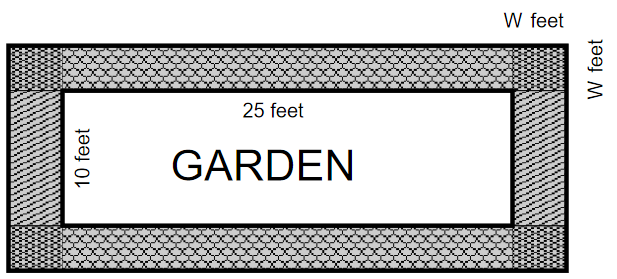
\includegraphics[width=\linewidth]{external/GravelPath.png}
\end{image}%
 The amount of gravel we need (\(G\) cubic feet) is given by the equation%
\begin{equation*}
G = W^2 + 17.5W
\end{equation*}
where \(W\) is the width of the path in feet. For example, a path 4 feet wide requires 86 cubic feet of gravel, as you can check.%
\begin{enumerate}[label=(\alph*),ref=\alph*]%
\item{}If the neighbor donates 60 cubic feet of gravel, how wide a path can they build? Set up and solve a quadratic equation to find the answer in feet, accurate to two decimal places. Then convert your answer into inches.%
\par\rule{\workspacestrutwidth}{0.7in}%
\item{}Gravel is measured by the \terminology{yard}, which is short for cubic yard. There are 27 cubic feet in 1 yard of gravel. If the neighbor donates three yards of gravel, how wide a path can they build? Set up and solve a quadratic equation to find the answer in feet, accurate to two decimal places. Then convert your answer into inches.%
\par\rule{\workspacestrutwidth}{0.7in}%
\item{}What would it mean to solve the equation to find where \(G=0\)? Can you tell what the answer is from the equation (without actually solving)?%
\par\rule{\workspacestrutwidth}{0in}%
\end{enumerate}%
\end{divisionexercise}%
\end{exercises-subsection-numberless}
\begin{conclusion}{When you're done \textellipsis{}}%
%
\begin{itemize}[label=\textbullet]
\item{}Check your solutions. Still confused? Work with a classmate, instructor, or tutor.%
\item{}Try the \alert{Do you know} questions. Not sure? Read the textbook and try again.%
\item{}Make a list of key ideas and processes to remember under \alert{Don't forget!}%
\item{}Do the textbook exercises and check your answers. Not sure if you are close enough? Compare answers with a classmate or ask your instructor or tutor.%
\item{}Getting the wrong answers or stuck? Re-read the section and try again. If you are still stuck, work with a classmate or go to your instructor's office hours or tutor hours.%
\item{}It is normal to find some parts of exercises difficult, but if most of them are a struggle, meet with your instructor or advisor about possible strategies or support services.%
\end{itemize}
%
\end{conclusion}%
\begin{conclusion}{Do you know \textellipsis{}}%
%
\begin{enumerate}[label={\Alph*.}]
\item{}What a ``quadratic'' function is?%
\item{}How to solve a quadratic equation?%
\item{}When we use the \hyperref[quadratic-formula]{Quadratic Formula}? \emph{Ask your instructor if you need to remember the \hyperref[quadratic-formula]{Quadratic Formula} or if it will be provided during the exam.}%
\item{}How to solve a quadratic equation when the function is not set equal to zero?%
\item{}How to identify the values of \(a, b, c\) in the formula?%
\item{}How to evaluate the formula (using your calculator)?%
\item{}Why there are (usually) two solutions to a quadratic equation?%
\item{}How to decide which solution(s) from the \hyperref[quadratic-formula]{Quadratic Formula} are correct?%
\item{}What the graph of a quadratic function looks like?%
\item{}The value for the independent variable to find the highest (or lowest) value of a quadratic function?%
\end{enumerate}
%
\par
\alert{Don't forget!}%
\end{conclusion}%
\end{sectionptx}
%
%
\typeout{************************************************}
\typeout{Section 3.6 Practice Exam 3A}
\typeout{************************************************}
%
\begin{sectionptx}{Section}{Practice Exam 3A}{}{Practice Exam 3A}{}{}{sec-PE3A}
%
%
\typeout{************************************************}
\typeout{Exercises 3.6 Practice Exam 3A}
\typeout{************************************************}
%
\begin{exercises-subsection-numberless}{Exercises}{Practice Exam 3A}{}{Practice Exam 3A}{}{}{ws-PE3A}
Relax. You have done problems like these before. Even if these problems look a bit different, just do what you can. If you're not sure of something, please ask! You may use your calculator. Please show all of your work and write down as many steps as you can. Don't spend too much time on any one problem. Do well. And remember, ask me if you're not sure about something.%
 \par
\terminology{Over 50 points on this exam are for solving equations and inequalities. Be sure you understand what you need to show for full credit. Using a different method will get little to no partial credit.}%
 \par
\emph{As you work, make a ``don't forget'' list of any information you need to look up or ask about.}%
 \begin{divisionexercise}{1}{}{}{well-linear-PE3A}%
The Skärstroms want to dig a new well for water for their lake cabin. The company charges \textdollar{}900 to bring the equipment on site and draw the permit and then \textdollar{}2 per foot to dig. That means%
\begin{equation*}
W=900+2F
\end{equation*}
where \(F\) is the depth of the well (in feet) and \(W\) is the cost of the well (in \textdollar{}).%
\begin{enumerate}[label=(\alph*),ref=\alph*]%
\item{}In their neck of the woods, wells often run 200 feet deep. According to the equation, how much would that cost?%
\par\rule{\workspacestrutwidth}{0.5in}%
\item{}The Skärstroms have budgeted between \textdollar{}1,500 and \textdollar{}1,800 for the well. Set up and solve a chain of inequalities to find the corresponding range of depths.%
\par\rule{\workspacestrutwidth}{1in}%
\item{}No such luck. The company had to drill much deeper than hoped to find water. The final result, wonderfully cold and clear drinking water. And, a hefty bill for \textdollar{}2,072. How deep is their well? Set up and solve an equation.%
\par\rule{\workspacestrutwidth}{0.5in}%
\end{enumerate}%
\end{divisionexercise}%
\clearpage
\begin{divisionexercise}{2}{}{}{caffeine-PE3A}%
Ceyda starts the day by downing two cans of Red Bull, containing a total of 160 mg of caffeine. Her body eliminates the caffeine at a rate of 12\% each hour. That means the amount of caffeine (\(C\) mg) after \(H\) hours is given by the equation graphed below%
\begin{equation*}
C= 160\ast 0.88^H
\end{equation*}
%
 \begin{image}{0}{1}{0}{}%
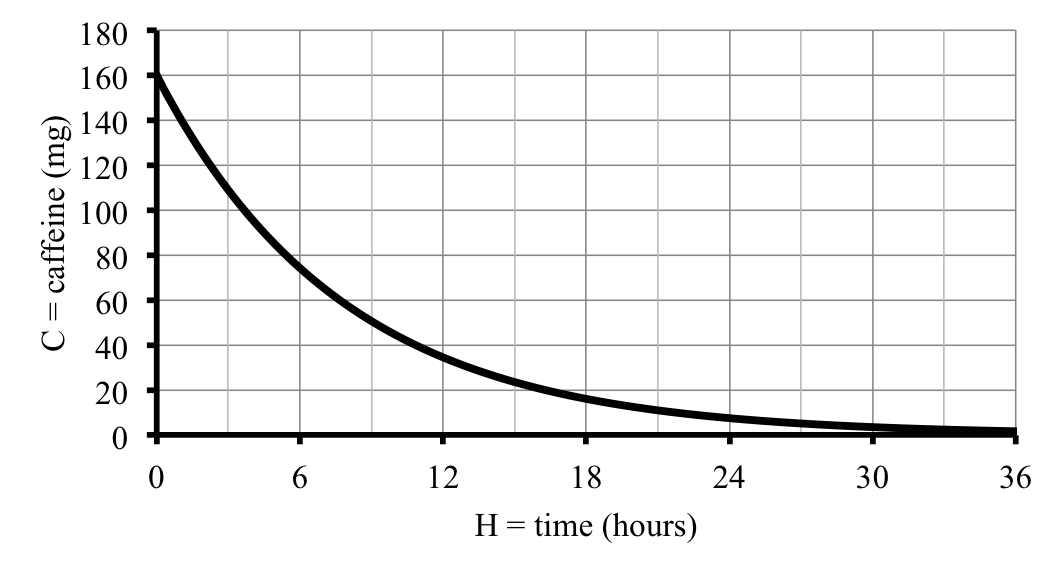
\includegraphics[width=\linewidth]{external/redbull.png}
\end{image}%
\begin{enumerate}[label=(\alph*),ref=\alph*]%
\item{}According to the equation, how much caffeine is in her body initially, after 2 hours, 5 hours, and 24 hours? Display your answers in table.%
\par\rule{\workspacestrutwidth}{0.5in}%
\item{}Show show to use successive approximation to find \emph{approximately} when Ceyda's caffeine level first drops below 20 mg. Answer to the nearest hour.%
\par\rule{\workspacestrutwidth}{1in}%
\item{}Set up and solve an equation to determine \emph{exactly} when Ceyda's caffeine level first drops below 20 mg. Round your answer to two decimal places.%
\par\rule{\workspacestrutwidth}{1in}%
\end{enumerate}%
\end{divisionexercise}%
\clearpage
\begin{divisionexercise}{3}{}{}{money-market-PE3A}%
Jorge deposited \textdollar{}1,500 in a high yield money market account and plans to leave it there for 5 years. The value of his account after 5 years, \textdollar{}\(A\), will depend on the growth factor \(g\) as given by the equation%
\begin{equation*}
A = 1,500\, g^5
\end{equation*}
%
\begin{enumerate}[label=(\alph*),ref=\alph*]%
\item{}Use the equation to complete the table.%
\begin{center}%
{\tabularfont%
\begin{tabular}{lllll}\hrulethin
\multicolumn{1}{AcA}{\(g\)}&\multicolumn{1}{cA}{1.02}&\multicolumn{1}{cA}{1.03}&\multicolumn{1}{cA}{1.05}&\multicolumn{1}{cA}{1.10}\tabularnewline\hrulethin
\multicolumn{1}{AcA}{\(A\)}&\multicolumn{1}{cA}{1,656.12}&\multicolumn{1}{cA}{\(\fillinmath{\begin{array}{c}XXXXX\\XXXXX\end{array}}\)}&\multicolumn{1}{cA}{\(\fillinmath{\begin{array}{c}XXXXX\\XXXXX\end{array}}\)}&\multicolumn{1}{cA}{2,415.77}\tabularnewline\hrulethin
\end{tabular}
}%
\end{center}%
\item{}Draw a graph showing how \(A\) depends on the growth factor \(g\). Start the horizontal axis at 1.00, instead of 0.%
\begin{image}{0.05}{0.9}{0.05}{}%

\includegraphics[width=\linewidth]{external/GraphPaper.jpg}
\end{image}%
\item{}Use your graph to \emph{estimate} the growth factor if the value of Jorge's account after 5 years is \textdollar{}1,780.%
\par\rule{\workspacestrutwidth}{0.25in}%
\item{}Now set up and solve an equation to find the answer \emph{exactly}.%
\par\rule{\workspacestrutwidth}{1in}%
\item{}What is the corresponding \terminology{return on investment}? That means calculate \(r= g-1\). The return on investment is \(r\) written as a percentage.%
\end{enumerate}%
\end{divisionexercise}%
\clearpage
\begin{divisionexercise}{4}{}{}{rabbit-jump-PE3A}%
A rabbit jumps so that her height above ground is given by the formula%
\begin{equation*}
R = 17.6T - 22T^2
\end{equation*}
where \(R=\) height of rabbit (feet above ground) and \(T=\) time (seconds).%
\begin{enumerate}[label=(\alph*),ref=\alph*]%
\item{}At what height did the rabbit start her jump?%
\par\rule{\workspacestrutwidth}{0.5in}%
\item{}Can the rabbit jump over a 3 foot fence? Calculate the exact maximum height of the rabbit to decide.%
\par\rule{\workspacestrutwidth}{1.5in}%
\item{}How long does it take the rabbit to get 2 feet in the air, and when is she at that height again? Set up and solve the appropriate equation to find the answers.%
\end{enumerate}%
\end{divisionexercise}%
\end{exercises-subsection-numberless}
\end{sectionptx}
%
%
\typeout{************************************************}
\typeout{Section 3.7 Practice Exam 3B}
\typeout{************************************************}
%
\begin{sectionptx}{Section}{Practice Exam 3B}{}{Practice Exam 3B}{}{}{sec-PE3B}
%
%
\typeout{************************************************}
\typeout{Exercises 3.7 Practice Exam 3B}
\typeout{************************************************}
%
\begin{exercises-subsection-numberless}{Exercises}{Practice Exam 3B}{}{Practice Exam 3B}{}{}{ws-PE3B}
\emph{Try taking this version of the practice exam under testing conditions: no book, no notes, no classmate's help, no electronics (computer, cell phone, television). Give yourself one hour to work and wait until you have tried your best on all of the problems before checking any answers.}%
 \par
\terminology{Caution:} Usually more than half points on this exam are for solving equations and inequalities. Be sure you understand what you need to show for full credit. Using a different method, or not showing enough work might get little to no partial credit.%
 \begin{divisionexercise}{1}{}{}{beanie-babies-PE3B}%
\begin{aside}{Aside}{}{beanie-babies-PE3B-1-1-1}%
These names are registered trademarked.%
\end{aside}
 Goldie the Goldfish, Pinches the Lobster, Quackers the Duck, Speedy the Turtle. These first generation Beanie Babies toys were anticipated to increase in value according to the equation%
\begin{equation*}
B = 6\ast 1.08^T
\end{equation*}
where \(B\) is the value of Beanie Babies (in \textdollar{}) and \(T\) is the time in years since 1994.%
\begin{enumerate}[label=(\alph*),ref=\alph*]%
\item{}Make a table showing the anticipated value in 1994, 2004, 2010, and 2025.%
\par\rule{\workspacestrutwidth}{1.25in}%
\item{}Draw a graph showing how the value of the Beanie Babies increased.%
\begin{image}{0.05}{0.9}{0.05}{}%

\includegraphics[width=\linewidth]{external/GraphPaper.jpg}
\end{image}%
~%
\item{}\emph{The problem continues \textellipsis{}}%
\par
Set up and solve an equation to determine when will Beanie Babies made in 1994 were anticipated to be worth over \textdollar{}40. Report the actual year.%
\end{enumerate}%
\end{divisionexercise}%
\clearpage
\begin{divisionexercise}{2}{}{}{porch-linear-PE3B}%
Best we can tell, the floor of our front porch was 7\textquotesingle{}2\textquotesingle\textquotesingle{} above ground when the house was built. It has been slowly sinking ever since. The contractor estimated that it's dropped 0.45 inches per year. The equation is%
\begin{equation*}
P = 86-0.45A
\end{equation*}
where \(P\) is the height of the porch (in inches) and \(A\) is the age of the house (in years).%
\begin{enumerate}[label=(\alph*),ref=\alph*]%
\item{}Make a table showing the height of the front porch when the house was built, when it was 20 years old, and when it was 50 years old.%
\par\rule{\workspacestrutwidth}{1.5in}%
\item{}The floor of our front porch is currently 48 inches above ground. Set up and solve an equation to figure out how old our house is.%
\par\rule{\workspacestrutwidth}{2in}%
\item{}Once the porch is below 40 inches, we will have to do something to fix it. Set up and solve an inequality to find when that will happen, answering to the nearest year. \emph{Hint: the house is already old. Report how many years from now.}%
\end{enumerate}%
\end{divisionexercise}%
\clearpage
\begin{divisionexercise}{3}{}{}{shot-put-PE3B}%
In a \terminology{shot put} competition, athletes try to throw a heavy metal ball as far as possible. For one athlete the ball closely followed the parabolic arch given by the equation%
\begin{equation*}
H = -0.015D^{2}+1.04D+5.9
\end{equation*}
where \(D\) was the distance the ball had travelled horizontally and \(H\) was the height of the ball above ground, both in feet. The path of the ball is graphed below.%
 \begin{image}{0}{1}{0}{}%
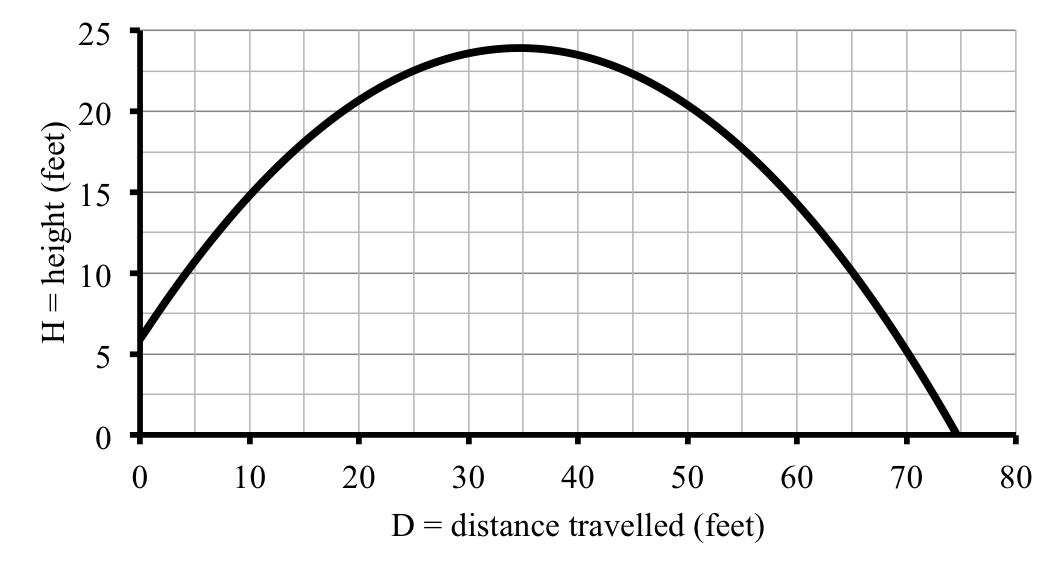
\includegraphics[width=\linewidth]{external/shotput.png}
\end{image}%
\begin{enumerate}[label=(\alph*),ref=\alph*]%
\item{}How far away did the ball land? Estimate the answer from the graph. Then show how to set up and solve an equation to find the answer to two decimal places.%
\par\rule{\workspacestrutwidth}{2.5in}%
\item{}How high up did the ball get? Show how to find the exact answer. Then compare to the graph.%
\end{enumerate}%
\end{divisionexercise}%
\clearpage
\begin{divisionexercise}{4}{}{}{volume-snowball-PE3B}%
The amount of snow in a snowball, \(C\) cups, depends on the \terminology{diameter} (distance across) of the snowball, \(D\) inches according to the equation%
\begin{equation*}
C = 0.036\, D^3
\end{equation*}
%
\begin{enumerate}[label=(\alph*),ref=\alph*]%
\item{}How many cups of snow are needed to make a snowball that is 3 inches across? 5 inches across?%
\par\rule{\workspacestrutwidth}{1in}%
\item{}How many cups of snow are needed to make a snowball that is 2 feet across? Give your answer in gallons. Use that 1 gallon = 4 quarts and 1 quart = 4 cups.%
\par\rule{\workspacestrutwidth}{1in}%
\item{}Karen has a 5 gallon paint bucket packed with snow and wants to make a giant snowball out of it. How big will the snowball be? Show how to use successive approximation to \emph{approximate} the answer to the nearest inch. Display your calculations in a table.%
\par\rule{\workspacestrutwidth}{1.5in}%
\item{}Now set up and solve an equation to find the answer \emph{exactly}, to the nearest inch.%
\end{enumerate}%
\end{divisionexercise}%
\end{exercises-subsection-numberless}
\end{sectionptx}
\end{chapterptx}
%
%
\typeout{************************************************}
\typeout{Chapter 4 A closer look at linear equations}
\typeout{************************************************}
%
\begin{chapterptx}{Chapter}{A closer look at linear equations}{}{A closer look at linear equations}{}{}{ch-4-Closer_look_linear}
\renewcommand*{\chaptername}{Chapter}
%
%
\typeout{************************************************}
\typeout{Section 4.1 Modeling with linear equations \textemdash{} Practice exercises}
\typeout{************************************************}
%
\begin{sectionptx}{Section}{Modeling with linear equations \textemdash{} Practice exercises}{}{Modeling with linear equations \textemdash{} Practice exercises}{}{}{sec-4-1-Modeling_linear_equations}
%
%
\typeout{************************************************}
\typeout{Exercises 4.1 Exercises}
\typeout{************************************************}
%
\begin{exercises-subsection-numberless}{Exercises}{Exercises}{}{Exercises}{}{}{ex-4-1-Modeling_linear_equations}
\begin{divisionexercise}{1}{}{}{solar-heating-modeling-linear}%
\begin{aside}{Aside}{}{solar-heating-modeling-linear-1-1-1}%
Source: ``Using Algebra'' by Ethan Bolker%
\par
(Story also appears in \hyperref[sec-4-2-Systems_linear_equations]{{\xreffont\ref{sec-4-2-Systems_linear_equations}}} Exercises)%
\end{aside}
 A solar heating system costs approximately \textdollar{}30,000 to install and \textdollar{}150 per year to run. By comparison, a gas heating system costs approximately \textdollar{}12,000 to install and \textdollar{}700 per year to run.%
\begin{enumerate}[label=(\alph*),ref=\alph*]%
\item{}What is the total cost for installing and running a gas heating system for 30 years?%
\par\rule{\workspacestrutwidth}{1in}%
\item{}Name variables and write a linear equation showing how the total cost for a gas heating system depends on the number of years you run it.%
\par\rule{\workspacestrutwidth}{1in}%
\item{}Name variables and write a linear equation showing how the total cost for a solar heating system depends on the number of years you run it.%
\par\rule{\workspacestrutwidth}{1in}%
\item{}If you install and run a solar heating system, how many years can you use it before it costs the same as installing and running a gas heating system for 30 years (your answer to part (a))? Set up and solve an equation.%
\par\rule{\workspacestrutwidth}{1in}%
\end{enumerate}%
\end{divisionexercise}%
\clearpage
\begin{divisionexercise}{2}{}{}{ebook-reader-modeling-linear}%
Since a very popular e-book reader was released, the price has been decreasing at a constant rate. A blogger developed the following equation representing the price \(E\) of the e-book reader \(T\) months since it was released:%
\begin{equation*}
E = 359 - 12T
\end{equation*}
%
\begin{enumerate}[label=(\alph*),ref=\alph*]%
\item{}Make a table of values for the e-book reader price initially, after 10 months, and after 25 months.%
\par\rule{\workspacestrutwidth}{0.75in}%
\item{}What does the 359 mean in the story and what are its units?%
\par\rule{\workspacestrutwidth}{0.75in}%
\item{}What does the 12 mean in the story and what are its units?%
\par\rule{\workspacestrutwidth}{0.75in}%
\item{}Draw a graph illustrating the dependence.%
\begin{image}{0.05}{0.9}{0.05}{}%

\includegraphics[width=\linewidth]{external/GraphPaper.jpg}
\end{image}%
\par\rule{\workspacestrutwidth}{0in}%
\item{}\emph{The problem continues \textellipsis{}}%
\par
After approximately how many months was the price of the e-book reader expected to be down to \textdollar{}200? Set up and solve an equation.%
\par\rule{\workspacestrutwidth}{2in}%
\item{}Sareth decided to purchase a e-book reader when the price fell below \textdollar{}100. How many months after its release did the price of the e-book reader fall below that level? Set up and solve an inequality.%
\par\rule{\workspacestrutwidth}{2in}%
\item{}If you can believe what you read in blogs, the manufacturer will soon be giving away the e-book reader for free, since they make money on the e-book sales themselves. How many months after it was released would that happen, according to our equation? Set up and solve an equation.%
\par\rule{\workspacestrutwidth}{2in}%
\end{enumerate}%
\end{divisionexercise}%
\clearpage
\begin{divisionexercise}{3}{}{}{ex-4-1-Modeling_linear_equations-3-1}%
Can you tell from the table which of these functions are linear? Use the rate of change to help you decide. Remember that these numbers may have been rounded.%
\begin{enumerate}[label=(\alph*),ref=\alph*]%
\item\label{grandfather-bonds-modeling-linear}Savings bonds from grandpa. \begin{aside}{Aside}{}{grandfather-bonds-modeling-linear-1-1-1}%
(Story also appears in \hyperref[sec-1-1-Variables_and_functions]{{\xreffont\ref{sec-1-1-Variables_and_functions}}} Exercises and \hyperlink{grandfather-bonds-growth-factor}{{\xreffont 5.3.1}})%
\end{aside}
%
\begin{center}%
{\tabularfont%
\begin{tabular}{lllllll}\hrulethin
\multicolumn{1}{AlA}{Year}&\multicolumn{1}{cA}{1962}&\multicolumn{1}{cA}{1970}&\multicolumn{1}{cA}{1980}&\multicolumn{1}{cA}{1990}&\multicolumn{1}{cA}{2000}&\multicolumn{1}{cA}{2010}\tabularnewline\hrulethin
\multicolumn{1}{AlA}{Value bond (\textdollar{})}&\multicolumn{1}{cA}{200.00}&\multicolumn{1}{cA}{318.77}&\multicolumn{1}{cA}{570.87}&\multicolumn{1}{cA}{1,022.34}&\multicolumn{1}{cA}{1,830.85}&\multicolumn{1}{cA}{3,278.77}\tabularnewline\hrulethin
\end{tabular}
}%
\end{center}%
\par\rule{\workspacestrutwidth}{1in}%
\item\label{wind-chill-modeling-linear}Wind chill at 10\textdegree{}F. \begin{aside}{Aside}{}{wind-chill-modeling-linear-1-1-2}%
(Story also appears in \hyperlink{wind-chill-tables-graphs}{{\xreffont 1.2.2}})%
\end{aside}
%
\begin{center}%
{\tabularfont%
\begin{tabular}{llllll}\hrulethin
\multicolumn{1}{AlA}{Wind (mph)}&\multicolumn{1}{cA}{0}&\multicolumn{1}{cA}{10}&\multicolumn{1}{cA}{20}&\multicolumn{1}{cA}{30}&\multicolumn{1}{cA}{40}\tabularnewline\hrulethin
\multicolumn{1}{AlA}{Wind chill (°F)}&\multicolumn{1}{cA}{10}&\multicolumn{1}{cA}{-4}&\multicolumn{1}{cA}{-9}&\multicolumn{1}{cA}{-12}&\multicolumn{1}{cA}{-15}\tabularnewline\hrulethin
\end{tabular}
}%
\end{center}%
\par\rule{\workspacestrutwidth}{1in}%
\item\label{pizza-diameter-modeling-linear}Pizza. \begin{aside}{Aside}{}{pizza-diameter-modeling-linear-1-1-1}%
(Story also appears in \hyperlink{pizza-diameter-powers-roots}{{\xreffont 0.6.2}}, \hyperlink{pizza-diameter-approx-solutions}{{\xreffont 2.4.1}}, and \hyperlink{pizza-diameter-solving-power}{{\xreffont 3.3.1}})%
\end{aside}
%
\begin{center}%
{\tabularfont%
\begin{tabular}{llll}\hrulethin
\multicolumn{1}{AlA}{Size (inches)}&\multicolumn{1}{cA}{8}&\multicolumn{1}{cA}{14}&\multicolumn{1}{cA}{16}\tabularnewline\hrulethin
\multicolumn{1}{AlA}{People}&\multicolumn{1}{cA}{1}&\multicolumn{1}{cA}{3}&\multicolumn{1}{cA}{4}\tabularnewline\hrulethin
\end{tabular}
}%
\end{center}%
\par\rule{\workspacestrutwidth}{1in}%
\item\label{reservoir-rain-modeling-linear}Water in the reservoir. \begin{aside}{Aside}{}{reservoir-rain-modeling-linear-1-1-1}%
(Story also appears in \hyperlink{reservoir-rain-first-look-linear}{{\xreffont 2.1.2}} and \hyperref[sec-3-2-Solving_linear_inequalities]{{\xreffont\ref{sec-3-2-Solving_linear_inequalities}}} Exercises)%
\end{aside}
%
\begin{center}%
{\tabularfont%
\begin{tabular}{lllll}\hrulethin
\multicolumn{1}{AlA}{Week}&\multicolumn{1}{cA}{1}&\multicolumn{1}{cA}{5}&\multicolumn{1}{cA}{10}&\multicolumn{1}{cA}{20}\tabularnewline\hrulethin
\multicolumn{1}{AlA}{Depth (feet)}&\multicolumn{1}{cA}{45.5}&\multicolumn{1}{cA}{39.5}&\multicolumn{1}{cA}{32}&\multicolumn{1}{cA}{17}\tabularnewline\hrulethin
\end{tabular}
}%
\end{center}%
\par\rule{\workspacestrutwidth}{1in}%
\end{enumerate}%
\end{divisionexercise}%
\clearpage
\begin{divisionexercise}{4}{}{}{plumber-rates-modeling-linear}%
Plumbers are really expensive, so I have been comparing prices. \begin{aside}{Aside}{}{plumber-rates-modeling-linear-1-1-1}%
(Story also appears in \hyperref[sec-2-1-First_look_linear]{{\xreffont\ref{sec-2-1-First_look_linear}}} Exercises)%
\end{aside}
 James charges \textdollar{}50 to show up plus \textdollar{}120 per hour. Jo is just getting started in the business. She charges \textdollar{}45 to show up plus \textdollar{}55 per hour. Mario advertises ``no trip charge'' but his hourly rate is \textdollar{}90 per hour. Not to be outdone, Luigi offers to unclog any drain for \textdollar{}150, no matter how long it takes. For each plumber, the table lists the corresponding equation and several points. In each equation, the plumber charges \textdollar{}\(P\) for \(T\) hours of work.%
 \begin{center}%
{\tabularfont%
\begin{tabular}{lllll}\hrulethin
\multicolumn{1}{AcA}{{\bfseries{}Plumber}}&\multicolumn{1}{cA}{{\bfseries{}James}}&\multicolumn{1}{cA}{{\bfseries{}Jo}}&\multicolumn{1}{cA}{{\bfseries{}Mario}}&\multicolumn{1}{cA}{{\bfseries{}Luigi}}\tabularnewline\hrulethin
\multicolumn{1}{AcA}{Equation}&\multicolumn{1}{cA}{\(P=50+120T\)}&\multicolumn{1}{cA}{\(P=45+55T\)}&\multicolumn{1}{cA}{\(P=90T\)}&\multicolumn{1}{cA}{\(P=150\)}\tabularnewline\hrulethin
\multicolumn{1}{AcA}{0 hours}&\multicolumn{1}{cA}{\textdollar{}50}&\multicolumn{1}{cA}{\textdollar{}45}&\multicolumn{1}{cA}{\textdollar{}0}&\multicolumn{1}{cA}{\textdollar{}150}\tabularnewline\hrulethin
\multicolumn{1}{AcA}{2 hours}&\multicolumn{1}{cA}{\textdollar{}290}&\multicolumn{1}{cA}{\textdollar{}155}&\multicolumn{1}{cA}{\textdollar{}180}&\multicolumn{1}{cA}{\textdollar{}150}\tabularnewline\hrulethin
\multicolumn{1}{AcA}{4 hours}&\multicolumn{1}{cA}{\textdollar{}530}&\multicolumn{1}{cA}{\textdollar{}265}&\multicolumn{1}{cA}{\textdollar{}360}&\multicolumn{1}{cA}{\textdollar{}150}\tabularnewline\hrulethin
\end{tabular}
}%
\end{center}%
\begin{enumerate}[label=(\alph*),ref=\alph*]%
\item{}Use the points given to plot each of the four lines on the same set of axes. Label each line with the plumber's name.%
\begin{image}{0.05}{0.9}{0.05}{}%

\includegraphics[width=\linewidth]{external/GraphPaper.jpg}
\end{image}%
\item{}What do you notice about Luigi's line?%
\par\rule{\workspacestrutwidth}{0.25in}%
\item{}List the plumbers in order from steepest to least steep line. What does that mean in terms of the story?%
\par\rule{\workspacestrutwidth}{0.25in}%
\item{}Now list the plumbers in order from smallest to largest intercept of their line. What does that mean in terms of the story?%
\par\rule{\workspacestrutwidth}{0.25in}%
\end{enumerate}%
\end{divisionexercise}%
\end{exercises-subsection-numberless}
\begin{conclusion}{When you're done \textellipsis{}}%
%
\begin{itemize}[label=\textbullet]
\item{}Check your solutions. Still confused? Work with a classmate, instructor, or tutor.%
\item{}Try the \alert{Do you know} questions. Not sure? Read the textbook and try again.%
\item{}Make a list of key ideas and processes to remember under \alert{Don't forget!}%
\item{}Do the textbook exercises and check your answers. Not sure if you are close enough? Compare answers with a classmate or ask your instructor or tutor.%
\item{}Getting the wrong answers or stuck? Re-read the section and try again. If you are still stuck, work with a classmate or go to your instructor's office hours or tutor hours.%
\item{}It is normal to find some parts of exercises difficult, but if most of them are a struggle, meet with your instructor or advisor about possible strategies or support services.%
\end{itemize}
%
\end{conclusion}%
\begin{conclusion}{Do you know \textellipsis{}}%
%
\begin{enumerate}[label={\Alph*.}]
\item{}What makes a function linear?%
\item{}What the slope of a linear function means in the story and what it tells us about the graph?%
\item{}What the intercept of a linear function means in the story and what it tells us about the graph?%
\item{}The template for a linear equation? \emph{Ask your instructor if you need to remember the template or if it will be provided during the exam.}%
\item{}How to write a linear equation given the starting amount (intercept) and the rate of change (slope)?%
\item{}Where the slope and intercept appear in the template of a linear equation?%
\item{}What the graph of a linear function looks like?%
\item{}How to solve a linear equation?%
\item{}Why the rate of change of a linear function is constant?%
\end{enumerate}
%
\par
\alert{Don't forget!}%
\end{conclusion}%
\end{sectionptx}
%
%
\typeout{************************************************}
\typeout{Section 4.2 Systems of linear equations - Practice exercises}
\typeout{************************************************}
%
\begin{sectionptx}{Section}{Systems of linear equations - Practice exercises}{}{Systems of linear equations - Practice exercises}{}{}{sec-4-2-Systems_linear_equations}
%
%
\typeout{************************************************}
\typeout{Exercises 4.2 Exercises}
\typeout{************************************************}
%
\begin{exercises-subsection-numberless}{Exercises}{Exercises}{}{Exercises}{}{}{ex-4-2-Systems_linear_equations}
\begin{divisionexercise}{1}{}{}{car-comparison-systems-linear}%
Madison wants to buy a new car, either Car A: a hybrid priced at \textdollar{}26,100, or Car B: a high-efficiency gas car priced at \textdollar{}23,700. Annual fuel costs for Car A are currently \textdollar{}1,100 per year. For Car B annual fuel costs are currently \textdollar{}1,800 per year. The total cost of each car will depend on how many years she keeps it.%
\begin{enumerate}[label=(\alph*),ref=\alph*]%
\item{}Name the variables.%
\par\rule{\workspacestrutwidth}{0.75in}%
\item{}Write a linear equation for the total cost (including purchase price and fuel costs) of \terminology{Car A} as a function of how long she keeps it. Assume fuel costs are constant.%
\par\rule{\workspacestrutwidth}{0.75in}%
\item{}Write a linear equation for the total cost (including purchase price and fuel costs) of \terminology{Car B} as a function of how long she keeps it. Assume fuel costs are constant.%
\par\rule{\workspacestrutwidth}{0.75in}%
\item{}Make a table comparing the total costs for the two cars if Madison keeps the car she buys for 3, 5, or 10 years.%
\par\rule{\workspacestrutwidth}{0.75in}%
\item{}Set up and solve a system of linear equations to determine the \terminology{payoff time}, or the number of years for which the total costs of each car are equal.%
\par\rule{\workspacestrutwidth}{0.75in}%
\item{}Based on what you have learned, fill in the blank: The more expensive hybrid pays off if Madison is going to keep it for \fillintext{3} years or more.%
\par\rule{\workspacestrutwidth}{0in}%
\end{enumerate}%
\end{divisionexercise}%
\clearpage
\begin{divisionexercise}{2}{}{}{juan-coffee-systems-linear}%
A mug of coffee costs \textdollar{}3.45 at Juan's favorite cafe, \begin{aside}{Aside}{}{juan-coffee-systems-linear-1-1-1}%
(Story also appears in \hyperlink{juan-coffee-order-operations}{{\xreffont 0.4.1}}, \hyperlink{juan-coffee-tables-graphs}{{\xreffont 1.2.4}}, and \hyperlink{juan-coffee-systems-linear}{{\xreffont 4.2.2}})%
\end{aside}
 unless he buys their discount card for \textdollar{}10 in which case a mug costs \textdollar{}2.90. Or, he can buy a membership for \textdollar{}59.99 and then coffee is only \textdollar{}1\slash{}mug. If we let \(M\) represent the number of mugs of coffee he buys and \(T\) represent the total cost in dollars, then the equations are:%
\begin{align*}
\textit{No card: } \qquad  
T \amp= 3.45M\\
\textit{With card: } \qquad  
T \amp= 10.00 + 2.90M\\
\textit{Membership: } \qquad  
T \amp= 59.99 + 1.00 M
\end{align*}
%
\begin{enumerate}[label=(\alph*),ref=\alph*]%
\item{}Compare the total costs for all three options.%
\begin{center}%
{\tabularfont%
\begin{tabular}{lllll}\hrulethin
\multicolumn{1}{AlA}{Mugs}&\multicolumn{1}{cA}{0}&\multicolumn{1}{cA}{10}&\multicolumn{1}{cA}{20}&\multicolumn{1}{cA}{30}\tabularnewline\hrulethin
\multicolumn{1}{AlA}{No card}&\multicolumn{1}{cA}{\(\fillinmath{\displaystyle\int\int\int}\)}&\multicolumn{1}{cA}{\(\fillinmath{\displaystyle\int\int\int}\)}&\multicolumn{1}{cA}{\(\fillinmath{\displaystyle\int\int\int}\)}&\multicolumn{1}{cA}{\(\fillinmath{\displaystyle\int\int\int}\)}\tabularnewline\hrulethin
\multicolumn{1}{AlA}{With card}&\multicolumn{1}{cA}{\(\fillinmath{\displaystyle\int\int\int}\)}&\multicolumn{1}{cA}{\(\fillinmath{\displaystyle\int\int\int}\)}&\multicolumn{1}{cA}{\(\fillinmath{\displaystyle\int\int\int}\)}&\multicolumn{1}{cA}{\(\fillinmath{\displaystyle\int\int\int}\)}\tabularnewline\hrulethin
\multicolumn{1}{AlA}{Member}&\multicolumn{1}{cA}{\(\fillinmath{\displaystyle\int\int\int}\)}&\multicolumn{1}{cA}{\(\fillinmath{\displaystyle\int\int\int}\)}&\multicolumn{1}{cA}{\(\fillinmath{\displaystyle\int\int\int}\)}&\multicolumn{1}{cA}{\(\fillinmath{\displaystyle\int\int\int}\)}\tabularnewline\hrulethin
\end{tabular}
}%
\end{center}%
\item{}Draw a graph showing all three options.%
\begin{image}{0.05}{0.9}{0.05}{}%

\includegraphics[width=\linewidth]{external/GraphPaper.jpg}
\end{image}%
\item{}Which option is least expensive if Juan plans to buy%
\par
%
\begin{itemize}[label=\textbullet]
\item{}A small number of mugs of coffee:%
\item{}A medium number of mugs of coffee:%
\item{}A large number of mugs of coffee:%
\end{itemize}
%
\par\rule{\workspacestrutwidth}{0.5cm}%
\item{}\emph{The problem continues \textellipsis{}}%
\par
Set up and solve a system of linear equations to compare total cost with no card to the total cost with the card.%
\par\rule{\workspacestrutwidth}{2.5in}%
\item{}Set up and solve a system of linear equation to compare the total cost with the card to the total cost with the membership.%
\par\rule{\workspacestrutwidth}{2.5in}%
\item{}Describe in words what you have learned.%
\par\rule{\workspacestrutwidth}{1in}%
\end{enumerate}%
\end{divisionexercise}%
\clearpage
\begin{divisionexercise}{3}{}{}{shrub-growth-systems-linear}%
Ahmed planted two shrubs in the backyard on May 1. \begin{aside}{Aside}{}{shrub-growth-systems-linear-1-1-1}%
(Story also appears in \hyperref[sec-4-1-Modeling_linear_equations]{{\xreffont\ref{sec-4-1-Modeling_linear_equations}}} Exercises)%
\end{aside}
 The viburnum was 16.9 inches tall and expected to grow 0.4 inches each week this summer. The weigela was 20.3 inches tall but only expected to grow 0.2 inches per week. If we let \(S\) represent the total height of the shrub in inches after \(T\) weeks, then the equations are:%
\begin{align*}
\textbf{Viburnum:} \qquad 
S \amp= 16.9 + 0.4T\\
\textbf{Weigela:} \qquad 
S \amp= 20.3 + 0.2T
\end{align*}
%
\begin{enumerate}[label=(\alph*),ref=\alph*]%
\item{}Compare the height of the shrubs on the given dates.%
\begin{center}%
{\tabularfont%
\begin{tabular}{lllll}\hrulethin
\multicolumn{1}{AlA}{date}&\multicolumn{1}{rA}{May 1}&\multicolumn{1}{rA}{June 12}&\multicolumn{1}{rA}{July 10}&\multicolumn{1}{rA}{Sept 4}\tabularnewline\hrulethin
\multicolumn{1}{AlA}{\(T\)}&\multicolumn{1}{rA}{0}&\multicolumn{1}{rA}{6}&\multicolumn{1}{rA}{10}&\multicolumn{1}{rA}{18}\tabularnewline\hrulethin
\multicolumn{1}{AlA}{\(S\) (viburnum)}&\multicolumn{1}{rA}{\(\fillinmath{\displaystyle\int\int\int}\)}&\multicolumn{1}{rA}{\(\fillinmath{\displaystyle\int\int\int}\)}&\multicolumn{1}{rA}{\(\fillinmath{\displaystyle\int\int\int}\)}&\multicolumn{1}{rA}{\(\fillinmath{\displaystyle\int\int\int}\)}\tabularnewline\hrulethin
\multicolumn{1}{AlA}{\(S\) (weigela)}&\multicolumn{1}{rA}{\(\fillinmath{\displaystyle\int\int\int}\)}&\multicolumn{1}{rA}{\(\fillinmath{\displaystyle\int\int\int}\)}&\multicolumn{1}{rA}{\(\fillinmath{\displaystyle\int\int\int}\)}&\multicolumn{1}{rA}{\(\fillinmath{\displaystyle\int\int\int}\)}\tabularnewline\hrulethin
\end{tabular}
}%
\end{center}%
\item{}\emph{Approximately} when will the shrubs be the same height? Continue successive approximation to find the answer to the nearest week.%
\par\rule{\workspacestrutwidth}{2in}%
\item{}Set up and solve an equation to find \emph{exactly} the day when the two shrubs are the same height. In what month does that happen?%
\par\rule{\workspacestrutwidth}{2in}%
\end{enumerate}%
\end{divisionexercise}%
\clearpage
\begin{divisionexercise}{4}{}{}{supply-demand-systems-linear}%
The \terminology{supply} of flour is the amount of flour produced. \begin{aside}{Aside}{}{supply-demand-systems-linear-1-1-2}%
Source: ``Using Algebra'' by Ethan Bolker%
\end{aside}
 It depends on the price of flour. A high price encourages producers to make more flour. If the price is low, they tend to make less of it. The dependence of the supply of flour \(S\) (in loads) on the price \(P\) (in \textdollar{}\slash{}pound) is given by the equation%
\begin{equation*}
\textbf{Supply: } S = 0.8P + 0.5
\end{equation*}
%
 \par
The \terminology{demand} of flour is the amount of flour consumers want to buy. It also depends on the price of flour. If flour sells for a high price, then consumers will buy less. If flour sells for a low price instead, then consumers will buy more. The dependence of the demand of flour \(D\) (in loads) on the price \(P\) (in \textdollar{}\slash{}pound) is given by the equation%
\begin{equation*}
\textbf{Demand: } D = 1.5 - 0.4 P
\end{equation*}
%
 \par
The \terminology{equilibrium price} of flour is the price where the supply equals the demand.%
\begin{enumerate}[label=(\alph*),ref=\alph*]%
\item{}What happens if flour is priced at \textdollar{}1.00\slash{}pound? That is, how much flour will be produced and how much will consumers demand?%
\par\rule{\workspacestrutwidth}{1cm}%
\item{}What happens if flour is priced at \textdollar{}0.50\slash{}pound? That is, how much flour will be produced and how much will consumers demand?%
\par\rule{\workspacestrutwidth}{1cm}%
\item{}Graph each dependence on the same set of axes. \emph{Approximately} what is the equilibrium price, according to your graph?%
\begin{image}{0.05}{0.9}{0.05}{}%

\includegraphics[width=\linewidth]{external/GraphPaper.jpg}
\end{image}%
\item{}\emph{The problem continues \textellipsis{}}%
\par
Set up and solve an equation to find the equilibrium price of flour \emph{exactly}.%
\par\rule{\workspacestrutwidth}{2in}%
\item{}When more of a product is produced than consumers want to buy, we have a \terminology{surplus} of the product. Solve an inequality to find the range of price values for which there will be a surplus of flour. Compare your answer to part (d).%
\par\rule{\workspacestrutwidth}{2in}%
\item{}When less of a product is produced than consumers want to buy, we have a \terminology{shortage} of the product. Solve an inequality to find the range of price values for which there will be a shortage of flour. Compare your answer to parts (d) and (e).%
\par\rule{\workspacestrutwidth}{2.2in}%
\end{enumerate}%
\end{divisionexercise}%
\end{exercises-subsection-numberless}
\begin{conclusion}{When you're done \textellipsis{}}%
%
\begin{itemize}[label=\textbullet]
\item{}Check your solutions. Still confused? Work with a classmate, instructor, or tutor.%
\item{}Try the \alert{Do you know} questions. Not sure? Read the textbook and try again.%
\item{}Make a list of key ideas and processes to remember under \alert{Don't forget!}%
\item{}Do the textbook exercises and check your answers. Not sure if you are close enough? Compare answers with a classmate or ask your instructor or tutor.%
\item{}Getting the wrong answers or stuck? Re-read the section and try again. If you are still stuck, work with a classmate or go to your instructor's office hours or tutor hours.%
\item{}It is normal to find some parts of exercises difficult, but if most of them are a struggle, meet with your instructor or advisor about possible strategies or support services.%
\end{itemize}
%
\end{conclusion}%
\begin{conclusion}{Do you know \textellipsis{}}%
%
\begin{enumerate}[label={\Alph*.}]
\item{}How to compare two linear functions using a table?%
\item{}How to graph two linear functions on the same axes?%
\item{}What the solution of a linear system means in terms of the story?%
\item{}Where to look on a graph to see the solution of a linear system?%
\item{}How to successively approximate the solution of a linear system?%
\item{}How to solve a linear system?%
\item{}When to use inequality instead of an equation for a linear system?%
\end{enumerate}
%
\par
\alert{Don't forget!}%
\end{conclusion}%
\end{sectionptx}
%
%
\typeout{************************************************}
\typeout{Section 4.3 Intercepts and direct proportionality - Practice exercises}
\typeout{************************************************}
%
\begin{sectionptx}{Section}{Intercepts and direct proportionality - Practice exercises}{}{Intercepts and direct proportionality - Practice exercises}{}{}{sec-4-3-Intercepts}
%
%
\typeout{************************************************}
\typeout{Exercises 4.3 Exercises}
\typeout{************************************************}
%
\begin{exercises-subsection-numberless}{Exercises}{Exercises}{}{Exercises}{}{}{ex-4-3-Intercepts}
\begin{divisionexercise}{1}{}{}{temperature-intercepts}%
In each of the following stories, the temperature changes over time. It might be confusing to call either variable \(T\), so use \(H\) for the time in hours and \(D\) for the temperature in degrees (°F). In each case, time should be measured from the start of the story.%
\begin{enumerate}[label=(\alph*),ref=\alph*]%
\item{}It was really cold at 8:30 this morning when Raina arrived at the office. Luckily the heating system warms things up very quickly, 4°F per hour. By 11:00 a.m. it was a very comfortable 72°F.%
\begin{enumerate}[label=\roman*.,ref=\theenumi.\roman*]%
\item{}Figure out what the temperature was at 8:30 a.m.%
\par\rule{\workspacestrutwidth}{1in}%
\item{}Write an equation illustrating the function.%
\par\rule{\workspacestrutwidth}{1in}%
\end{enumerate}%
\item{}While 72°F is a perfectly good temperature for an office, not so for ballroom dancing. When Raina arrived for her practice at 5:30 that evening, she began to sweat before she even took the floor. Turns out the air conditioner had been running since 4:00 p.m. but it only cools down the room 3°F per hour.%
\begin{enumerate}[label=\roman*.,ref=\theenumi.\roman*]%
\item{}Figure out what the temperature was at 4:00 p.m.%
\par\rule{\workspacestrutwidth}{1in}%
\item{}Write an equation illustrating the function.%
\par\rule{\workspacestrutwidth}{1in}%
\end{enumerate}%
\end{enumerate}%
\end{divisionexercise}%
\clearpage
\begin{divisionexercise}{2}{}{}{design-business-intercepts}%
Maryn is very happy. Her interior design business is finally showing a profit. She has logged a total of 471 billable hours at \textdollar{}35 per hour since she started her business. Accounting for start up costs, her net profit now totals \textdollar{}2,194.%
\begin{enumerate}[label=(\alph*),ref=\alph*]%
\item{}How much were Maryn's start up costs?%
\par\rule{\workspacestrutwidth}{1.4cm}%
\item{}Identify the slope and intercept (including their units and sign) and explain what each means in terms of the story.%
\par\rule{\workspacestrutwidth}{1.4cm}%
\item{}Calculate what Maryn's profits will be once she has logged a total of 1,000 hours.%
\par\rule{\workspacestrutwidth}{1.4cm}%
\item{}Name the variables and write an equation relating them.%
\par\rule{\workspacestrutwidth}{1.4cm}%
\item{}Graph the function.%
\begin{image}{0.05}{0.9}{0.05}{}%

\includegraphics[width=\linewidth]{external/GraphPaper.jpg}
\end{image}%
\par\rule{\workspacestrutwidth}{0in}%
\end{enumerate}%
\end{divisionexercise}%
\clearpage
\begin{divisionexercise}{3}{}{}{weight-change-intercepts}%
For each story, find the initial weight of the person, \begin{aside}{Aside}{}{weight-change-intercepts-1-1-1}%
(Stories also appear in \hyperlink{weight-change-order-operations}{{\xreffont 0.4.3}} and \hyperlink{weight-change-algebraic-notation}{{\xreffont 0.7.1}})%
\end{aside}
 and use it to write an equation showing how the person's weight \(W\) pounds depends on the time, \(T\) weeks.%
\begin{enumerate}[label=(\alph*),ref=\alph*]%
\item{}Jerome has gained weight since he took his power training to the next level ten weeks ago, at the rate of around 1 pound a week. He now weighs 198 pounds.%
\par\rule{\workspacestrutwidth}{1.3in}%
\item{}Vanessa's doctor put her on a sensible diet and exercise plan to get her back to a healthy weight. She will need to lose an average of 1.25 pounds a week to reach her goal weight of 148 pounds in a year. Use 1 year = 52 weeks.%
\par\rule{\workspacestrutwidth}{1.3in}%
\item{}After the past 6 weeks of terrible migrane headaches, Carlos is down to 158 pounds. He has lost 4 pounds a week.%
\par\rule{\workspacestrutwidth}{1.3in}%
\item{}Since she has been pregnant, Zoe has gained the recommended \(\sfrac{1}{2}\) pound per week. Now 30 weeks pregnant and 168 pounds, she wonders if she will ever see her feet again.%
\par\rule{\workspacestrutwidth}{1.3in}%
\end{enumerate}%
\end{divisionexercise}%
\clearpage
\begin{divisionexercise}{4}{}{}{proportional-intercepts}%
Each story describes a situation that we are assuming is linear. Decide whether it is \terminology{proportional}, meaning the intercept equals zero. If it is proportional, explain why the intercept would be zero. If it is not proportional, explain what the intercept would mean in the story.%
\begin{enumerate}[label=(\alph*),ref=\alph*]%
\item{}The price of \terminology{kiwis} (a kind of fruit) depends on how many kiwis you buy.%
\par\rule{\workspacestrutwidth}{1in}%
\item{}The price of a bag of tortillas depends on how many tortillas are in the bag.%
\par\rule{\workspacestrutwidth}{1in}%
\item{}The time it takes to vacuum a rug depends on the area of the rug.%
\par\rule{\workspacestrutwidth}{1in}%
\item{}The time it takes to wash dishes depends on how many dirty dishes there are.%
\par\rule{\workspacestrutwidth}{1in}%
\item{}The amount of laundry detergent I have left depends on how many loads of laundry I did.%
\par\rule{\workspacestrutwidth}{1.25in}%
\end{enumerate}%
\end{divisionexercise}%
\end{exercises-subsection-numberless}
\begin{conclusion}{When you're done \textellipsis{}}%
%
\begin{itemize}[label=\textbullet]
\item{}Check your solutions. Still confused? Work with a classmate, instructor, or tutor.%
\item{}Try the \alert{Do you know} questions. Not sure? Read the textbook and try again.%
\item{}Make a list of key ideas and processes to remember under \alert{Don't forget!}%
\item{}Do the textbook exercises and check your answers. Not sure if you are close enough? Compare answers with a classmate or ask your instructor or tutor.%
\item{}Getting the wrong answers or stuck? Re-read the section and try again. If you are still stuck, work with a classmate or go to your instructor's office hours or tutor hours.%
\item{}It is normal to find some parts of exercises difficult, but if most of them are a struggle, meet with your instructor or advisor about possible strategies or support services.%
\end{itemize}
%
\end{conclusion}%
\begin{conclusion}{Do you know \textellipsis{}}%
%
\begin{enumerate}[label={\Alph*.}]
\item{}What the intercept of a linear function means in the story and what it tells us about the graph?%
\item{}How to calculate the intercept given the slope and an example (another point on the graph)?%
\item{}Why an intercept might not make sense, for example if it's outside the domain of the function?%
\item{}When a linear function is a direct proportion?%
\item{}Why you cannot reason proportionally if the linear function is not a direct proportion?%
\item{}What the graph of a direct proportion looks like?%
\end{enumerate}
%
\par
\alert{Don't forget!}%
\end{conclusion}%
\end{sectionptx}
%
%
\typeout{************************************************}
\typeout{Section 4.4 Slopes - Practice exercises}
\typeout{************************************************}
%
\begin{sectionptx}{Section}{Slopes - Practice exercises}{}{Slopes - Practice exercises}{}{}{sec-4-4-Slopes}
%
%
\typeout{************************************************}
\typeout{Exercises 4.4 Exercises}
\typeout{************************************************}
%
\begin{exercises-subsection-numberless}{Exercises}{Exercises}{}{Exercises}{}{}{ex-4-4-Slopes}
\begin{divisionexercise}{1}{}{}{wings-delivery-slopes}%
For his Oscars party, Harland had 70 chicken wings delivered for \textdollar{}51.25. For his Super Bowl bash, Harland had 125 chicken wings delivered for \textdollar{}83.70. In each case, the total cost includes the cost per wing and the fixed delivery charge.%
\begin{enumerate}[label=(\alph*),ref=\alph*]%
\item{}Find the slope, including units, and explain what it means in the story.%
\par\rule{\workspacestrutwidth}{1cm}%
\item{}Find the intercept, including units, and explain what it means in the story.%
\par\rule{\workspacestrutwidth}{1cm}%
\item{}Name the variables and write an equation for the function.%
\par\rule{\workspacestrutwidth}{1cm}%
\item{}How many wings could Harland order for \textdollar{}100? Solve your equation.%
\par\rule{\workspacestrutwidth}{2cm}%
\item{}Graph and check.%
\begin{image}{0.05}{0.9}{0.05}{}%

\includegraphics[width=\linewidth]{external/GraphPaper.jpg}
\end{image}%
\par\rule{\workspacestrutwidth}{0in}%
\end{enumerate}%
\end{divisionexercise}%
\clearpage
\begin{divisionexercise}{2}{}{}{leather-belts-slopes}%
Jana is making belts out of leather strips and a metal clasp. A short belt (as shown) is 24.5 inches long and includes 7 leather strips. A long belt (not shown) is 37.3 inches long and includes 11 leather strips. Each belt includes one metal clasp that is part of the total length. All belts use the same length clasp.%
 \begin{image}{0}{1}{0}{}%

\includegraphics[width=\linewidth]{external/leatherbelt.png}
\end{image}%
\begin{enumerate}[label=(\alph*),ref=\alph*]%
\item{}Name the variables, including units.%
\par\rule{\workspacestrutwidth}{0.75in}%
\item{}How long is each leather strip?%
\par\rule{\workspacestrutwidth}{0.75in}%
\item{}How long is the metal clasp?%
\par\rule{\workspacestrutwidth}{0.75in}%
\item{}Write an equation relating the variables.%
\par\rule{\workspacestrutwidth}{0.75in}%
\item{}Solve your equation to find the number of leather strips in an extra long belt that is 43.7 inches long.%
\par\rule{\workspacestrutwidth}{0.75in}%
\end{enumerate}%
\end{divisionexercise}%
\clearpage
\begin{divisionexercise}{3}{}{}{ski-passes-slopes}%
The local ski resort is trying to set the price for season passes. They know from past experience that they will sell around 14,000 passes if the season ticket price is \textdollar{}380. If the price is \textdollar{}400, they will sell fewer, perhaps only 11,000 passes. You can assume this decrease in demand is linear.%
\begin{enumerate}[label=(\alph*),ref=\alph*]%
\item{}Name the variables, including units and dependence.%
\par\rule{\workspacestrutwidth}{0.6in}%
\item{}For every dollar increase in price, how many fewer people purchase season passes?%
\par\rule{\workspacestrutwidth}{0.75in}%
\item{}Find the intercept. Explain why this number does not make sense in the problem.%
\par\rule{\workspacestrutwidth}{0.75in}%
\item{}Write an equation for the function. %
\par\rule{\workspacestrutwidth}{0.75in}%
\item{}How many season passes will they sell if the price is reduced to \textdollar{}355?%
\par\rule{\workspacestrutwidth}{0.75in}%
\item{}The ski resort can compute the \terminology{revenue} (total amount of money they take in) by multiplying the ticket price times the number of tickets sold. Calculate the revenue when ticket prices are \textdollar{}355, \textdollar{}380, and \textdollar{}400. %
\par\rule{\workspacestrutwidth}{0.75in}%
\item{}Of these three prices, which yields the most revenue?%
\par\rule{\workspacestrutwidth}{0in}%
\end{enumerate}%
\end{divisionexercise}%
\clearpage
\begin{divisionexercise}{4}{}{}{press-weight-slopes}%
Boy, am I out of shape. Right now I can only press about 15 pounds. (\terminology{Press} means lift weight off my chest. Literally.) My trainer says I should be able to press 50 pounds by the end of 10 weeks of serious lifting. I plan to increase the weight I press by a fixed amount each week.%
\begin{enumerate}[label=(\alph*),ref=\alph*]%
\item{}Name the variables and write an equation for my trainer's projection. \emph{Hint: You already know the intercept.}%
\par\rule{\workspacestrutwidth}{2in}%
\item{}Make a table showing my trainer's projection for after 0, 5, 10, 15, and 20 weeks.%
\par\rule{\workspacestrutwidth}{2in}%
\item{}Years ago I could press 90 pounds. At this rate, when will I be able to press at least 90 pounds again? Set up and solve an inequality.%
\par\rule{\workspacestrutwidth}{2.2in}%
\item{}\emph{The problem continues \textellipsis{}}%
\par
Draw a graph illustrating the function.%
\begin{image}{0.05}{0.9}{0.05}{}%

\includegraphics[width=\linewidth]{external/GraphPaper.jpg}
\end{image}%
\par\rule{\workspacestrutwidth}{0in}%
\item{}I am skeptical. I do not think I will be able to press 50 pounds by the end of 10 weeks. If I revise my equation, would my new slope be larger or smaller?%
\par
\emph{Hint: Try sketching in a possible revised line on your graph assuming that after 10 weeks I will press much less than 50 pounds.}%
\par\rule{\workspacestrutwidth}{1.5in}%
\item{}Will my revised projections mean I will reach that 90-pound goal sooner or later than my trainer thinks? Explain. \emph{Hint: extend your graph.}%
\par\rule{\workspacestrutwidth}{1.25in}%
\end{enumerate}%
\end{divisionexercise}%
\end{exercises-subsection-numberless}
\begin{conclusion}{When you're done \textellipsis{}}%
%
\begin{itemize}[label=\textbullet]
\item{}Check your solutions. Still confused? Work with a classmate, instructor, or tutor.%
\item{}Try the \alert{Do you know} questions. Not sure? Read the textbook and try again.%
\item{}Make a list of key ideas and processes to remember under \alert{Don't forget!}%
\item{}Do the textbook exercises and check your answers. Not sure if you are close enough? Compare answers with a classmate or ask your instructor or tutor.%
\item{}Getting the wrong answers or stuck? Re-read the section and try again. If you are still stuck, work with a classmate or go to your instructor's office hours or tutor hours.%
\item{}It is normal to find some parts of exercises difficult, but if most of them are a struggle, meet with your instructor or advisor about possible strategies or support services.%
\end{itemize}
%
\end{conclusion}%
\begin{conclusion}{Do you know \textellipsis{}}%
%
\begin{enumerate}[label={\Alph*.}]
\item{}Which types of situations are linear?%
\item{}What the slope of a linear function means in the story and what it tells us about the graph?%
\item{}How to calculate the slope between two points?%
\item{}What it means if the slope is negative?%
\item{}How to find the equation of a line through two points?%
\item{}How to find a linear function given two examples in a story?%
\item{}If both the slope and intercept are unknown, which is easier to calculate first?%
\end{enumerate}
%
\par
\alert{Don't forget!}%
\end{conclusion}%
\end{sectionptx}
%
%
\typeout{************************************************}
\typeout{Section 4.5 Fitting lines to data - Practice exercises}
\typeout{************************************************}
%
\begin{sectionptx}{Section}{Fitting lines to data - Practice exercises}{}{Fitting lines to data - Practice exercises}{}{}{sec-4-5-Fitting_lines_to_data}
%
%
\typeout{************************************************}
\typeout{Exercises 4.5 Exercises}
\typeout{************************************************}
%
\begin{exercises-subsection-numberless}{Exercises}{Exercises}{}{Exercises}{}{}{ex-4-5-Fitting_lines_to_data}
\begin{divisionexercise}{1}{}{}{wood-volume-fitting-lines}%
The scatter plot shows the total volume of wood, \(V\) cubic feet, in managed forests of different ages, \(A\) years.%
\begin{enumerate}[label=(\alph*),ref=\alph*]%
\item{}For each line, state some reason why the fit is not good. (We know the line will not go through all, or even most, of the points, so that is not the problem. Instead look at slope\slash{}steepness, intercept\slash{}height, etc.)%
\begin{sidebyside}{2}{0}{0}{0}%
\begin{sbspanel}{0.5}%
Line A%
\par
\noindent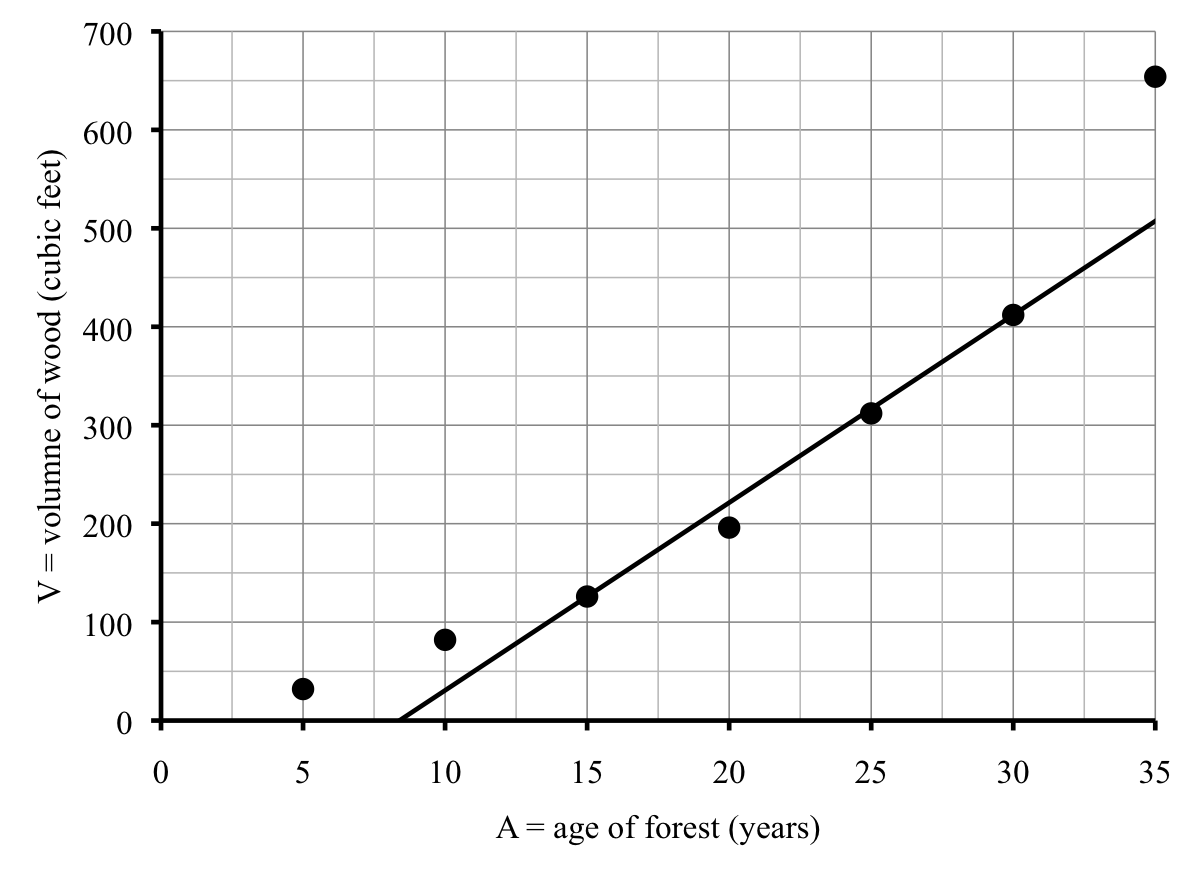
\includegraphics[width=\linewidth]{external/woodforestA.png}
\end{sbspanel}%
\begin{sbspanel}{0.5}%
Line B%
\par
\noindent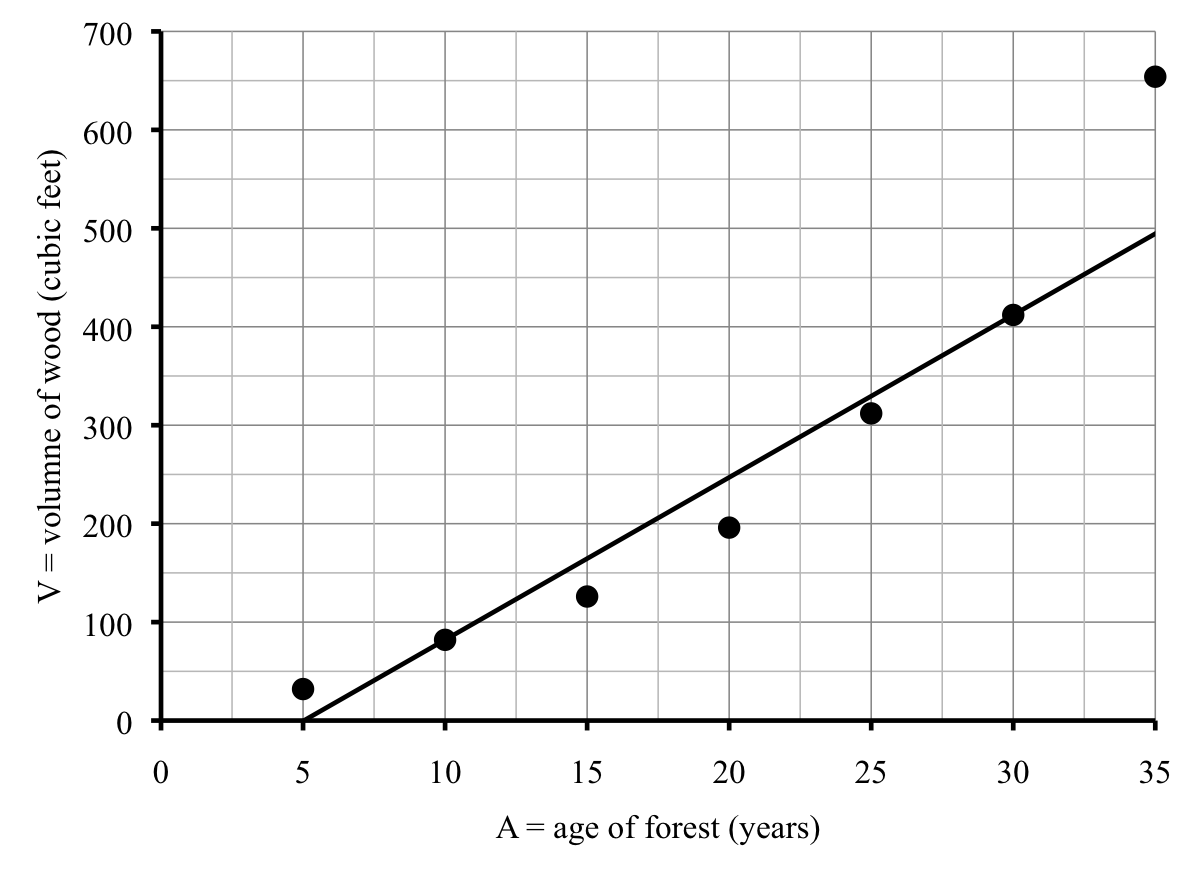
\includegraphics[width=\linewidth]{external/woodforestC.png}
\end{sbspanel}%
\end{sidebyside}%
\par
~%
\par
~%
\par
~%
\par
~%
\begin{sidebyside}{2}{0}{0}{0}%
\begin{sbspanel}{0.5}%
Line C%
\par
\noindent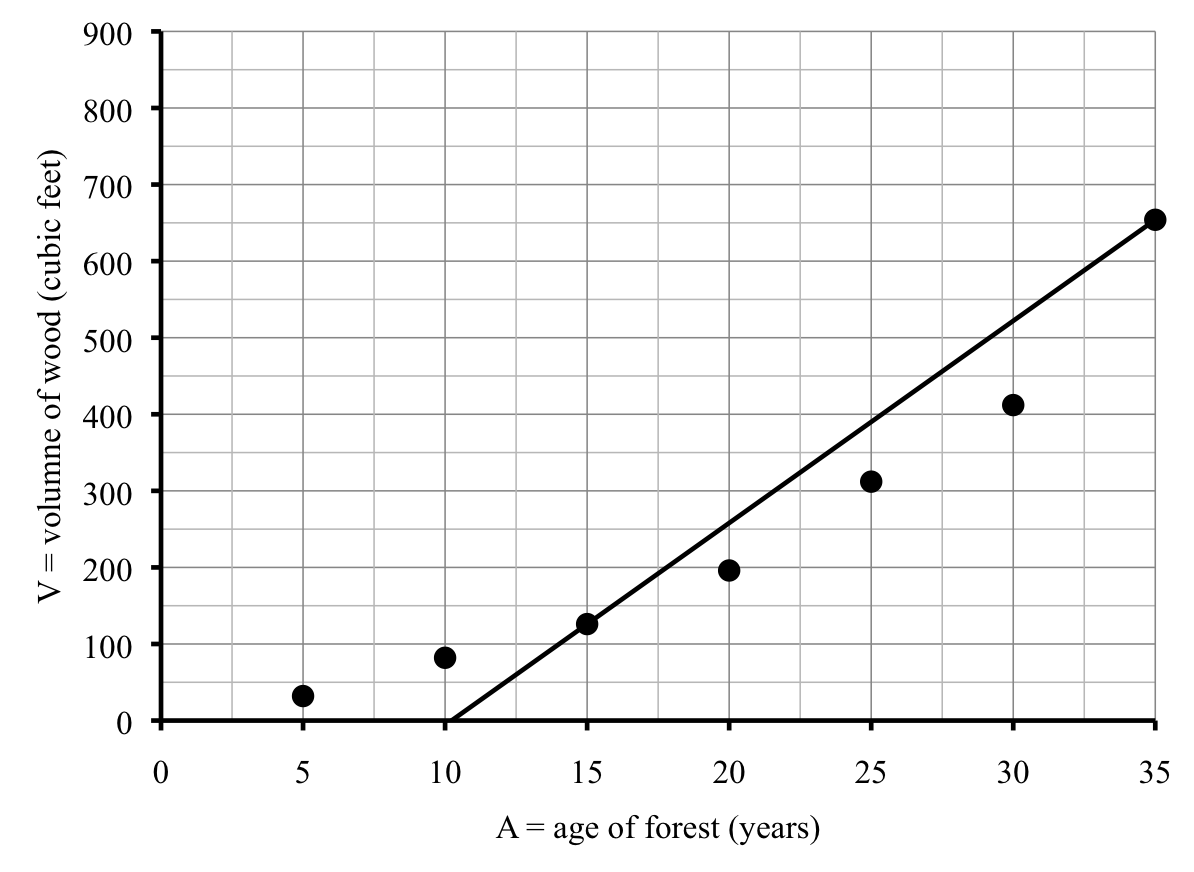
\includegraphics[width=\linewidth]{external/woodforestD.png}
\end{sbspanel}%
\begin{sbspanel}{0.5}%
Line D%
\par
\noindent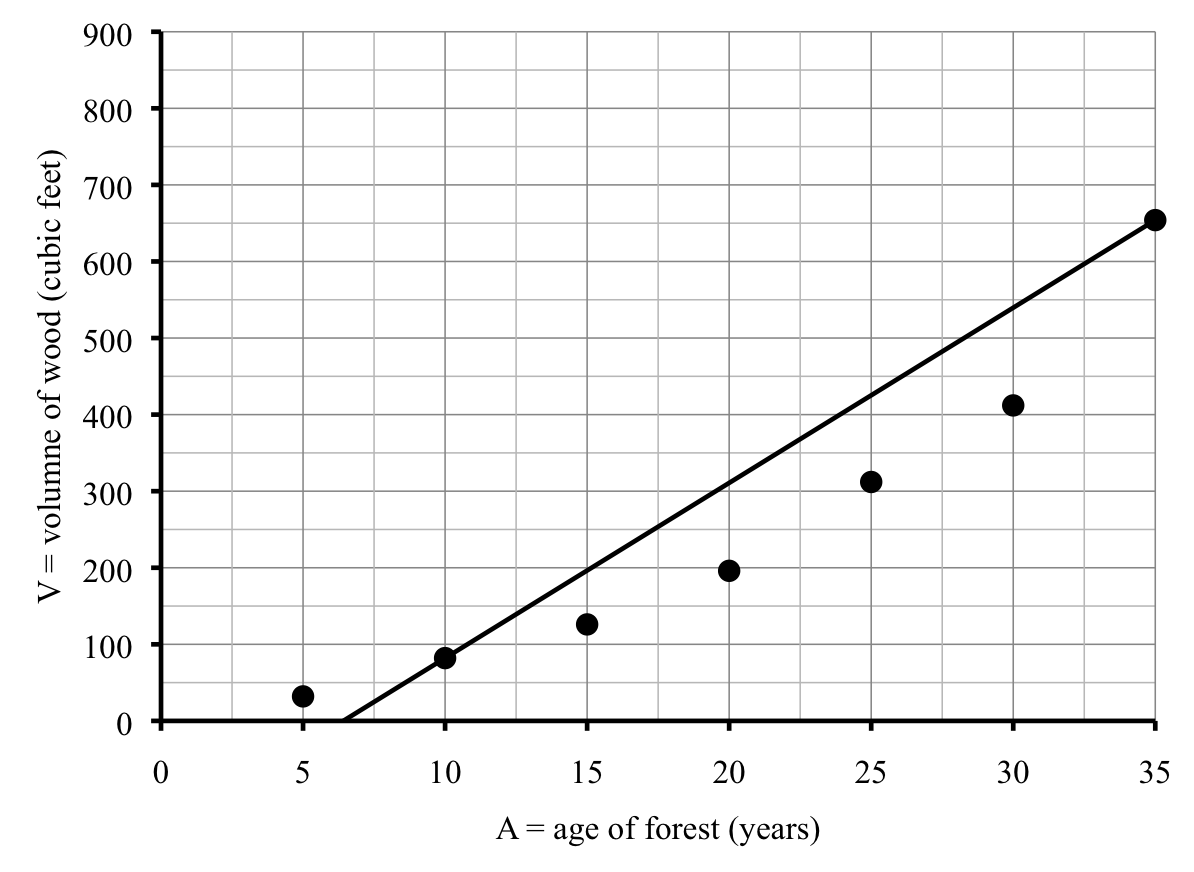
\includegraphics[width=\linewidth]{external/woodforestE.png}
\end{sbspanel}%
\end{sidebyside}%
\par
~%
\par
~%
\par
~%
\par
~%
\item{}Which of these four lines do you think fits best, and why?%
\end{enumerate}%
\end{divisionexercise}%
\clearpage
\begin{divisionexercise}{2}{}{}{stock-price-fitting-lines}%
Noel is considering investing in a company's stock so he looked up a few values.%
 \begin{center}%
{\tabularfont%
\begin{tabular}{llll}\hrulethin
\multicolumn{1}{AlA}{Day}&\multicolumn{1}{cA}{0}&\multicolumn{1}{cA}{300}&\multicolumn{1}{cA}{500}\tabularnewline\hrulethin
\multicolumn{1}{AlA}{Value (\textdollar{})}&\multicolumn{1}{cA}{23.19}&\multicolumn{1}{cA}{37.00}&\multicolumn{1}{cA}{48.10}\tabularnewline\hrulethin
\end{tabular}
}%
\end{center}%
\begin{enumerate}[label=(\alph*),ref=\alph*]%
\item{}Calculate the daily rate of change of the stock's price during the first 300 days.%
\par\rule{\workspacestrutwidth}{0.65in}%
\item{}Calculate the daily rate of change of the stock's price from Day 300 to Day 500.%
\par\rule{\workspacestrutwidth}{0.65in}%
\item{}Is this growth linear? How do you know?%
\par\rule{\workspacestrutwidth}{0.25in}%
\item{}The scatter plot shows additional values of the stock Noel is considering buying.%
\begin{image}{0}{1}{0}{}%
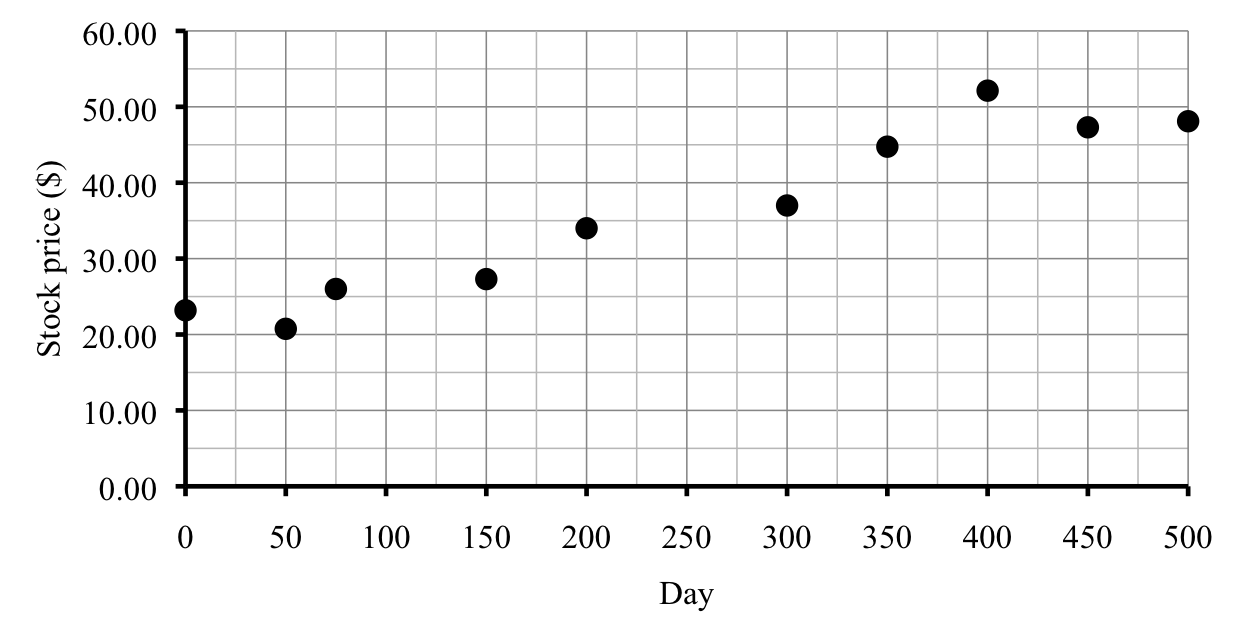
\includegraphics[width=\linewidth]{external/stockprices.png}
\end{image}%
Draw in a line through the points for Day 300 and Day 500. Label this line \#1. Explain why that line does not fit the data well.%
\par\rule{\workspacestrutwidth}{0.65in}%
\item{}Draw in a line that fits the data better. It does not need to go through any of the points exactly. Label that line \#2.%
\par\rule{\workspacestrutwidth}{0in}%
\end{enumerate}%
\end{divisionexercise}%
\clearpage
\begin{divisionexercise}{3}{}{}{work-gpa-fitting-lines}%
Is it true that students who work part-time have lower grades? Do the number of hours matter? The table shows the grade point average (GPA) of ten students compared to the number of hours per week each student works at a part time job. The variables we used are \(T\), for the time worked at job (hours\slash{}week), and \(G\) for the GPA, on the usual scale of 0.0 to 4.0.%
 \begin{center}%
{\tabularfont%
\begin{tabular}{lllllllllll}\hrulethin
\multicolumn{1}{AcA}{\(T\)}&\multicolumn{1}{cA}{0}&\multicolumn{1}{cA}{0}&\multicolumn{1}{cA}{10}&\multicolumn{1}{cA}{12}&\multicolumn{1}{cA}{14}&\multicolumn{1}{cA}{15}&\multicolumn{1}{cA}{16}&\multicolumn{1}{cA}{18}&\multicolumn{1}{cA}{20}&\multicolumn{1}{cA}{20}\tabularnewline\hrulethin
\multicolumn{1}{AcA}{\(G\)}&\multicolumn{1}{cA}{3.72}&\multicolumn{1}{cA}{3.91}&\multicolumn{1}{cA}{3.43}&\multicolumn{1}{cA}{2.79}&\multicolumn{1}{cA}{3.08}&\multicolumn{1}{cA}{2.62}&\multicolumn{1}{cA}{2.44}&\multicolumn{1}{cA}{3.17}&\multicolumn{1}{cA}{3.00}&\multicolumn{1}{cA}{2.55}\tabularnewline\hrulethin
\end{tabular}
}%
\end{center}%
\begin{enumerate}[label=(\alph*),ref=\alph*]%
\item{}Make a scatter plot of the points. Start the \(G\)-axis at 2.0.%
\begin{image}{0.05}{0.9}{0.05}{}%

\includegraphics[width=\linewidth]{external/GraphPaper.jpg}
\end{image}%
\item{}Find the equation of the line that goes through the first and last point listed.%
\par
\emph{Hint: the first point tells you the intercept.}%
\par\rule{\workspacestrutwidth}{2.5in}%
\item{}Draw this line on your graph and label it line A.%
\item{}\emph{The problem continues \textellipsis{}}%
\par
Use your equation for line A to figure out what you would expect for the GPA of a student working 30 hours per week.%
\par\rule{\workspacestrutwidth}{1in}%
\item{}It turns out, the best fitting line has equation \(G=3.7597-0.0551T\). Make a table of values for this equation using \(T=0, 10, 20\) hours.%
\par\rule{\workspacestrutwidth}{2in}%
\item{}Use that table of values to graph this best fitting line on that same set of axes. Label it line B.%
\item{}According to line B, what is the greatest number of hours a student should work if they want to maintain a 3.5 GPA? Solve an equation, then check on your graph.%
\end{enumerate}%
\end{divisionexercise}%
\clearpage
\begin{divisionexercise}{4}{}{}{candy-shop-fitting-lines}%
Mia and Mandi and opened a candy shop this January. The table shows their monthly sales profit. Except for some seasonal fluctuation, Mia and Mandi generally expect your profits to rise steadily while their business is getting established.%
 \begin{center}%
{\tabularfont%
\begin{tabular}{lllllllll}\hrulethin
\multicolumn{1}{AcA}{Month}&\multicolumn{1}{cA}{Jan}&\multicolumn{1}{cA}{Feb}&\multicolumn{1}{cA}{Mar}&\multicolumn{1}{cA}{Apr}&\multicolumn{1}{cA}{May}&\multicolumn{1}{cA}{Jun}&\multicolumn{1}{cA}{Jul}&\multicolumn{1}{cA}{Aug}\tabularnewline\hrulethin
\multicolumn{1}{AcA}{Sales Profit (\textdollar{})}&\multicolumn{1}{cA}{3,394}&\multicolumn{1}{cA}{4,702}&\multicolumn{1}{cA}{3,683}&\multicolumn{1}{cA}{4,840}&\multicolumn{1}{cA}{5,632}&\multicolumn{1}{cA}{4,432}&\multicolumn{1}{cA}{4,649}&\multicolumn{1}{cA}{4,590}\tabularnewline\hrulethin
\end{tabular}
}%
\end{center}%
\begin{enumerate}[label=(\alph*),ref=\alph*]%
\item{}Make a scatter plot. Begin the profit axis at \textdollar{}3,000.%
\begin{image}{0.05}{0.9}{0.05}{}%

\includegraphics[width=\linewidth]{external/GraphPaper.jpg}
\end{image}%
\item{}Name the variables and write an equation for the line through January and August. Add this line (\#1) to your graph. This line is too low.%
\par\rule{\workspacestrutwidth}{8cm}%
\item{}\emph{The problem continues \textellipsis{}}%
\par
Write an equation for the line through March and July. Notice that you need to find the intercept this time. Add this line (\#2) to your graph. This line is too steep.%
\par\rule{\workspacestrutwidth}{3in}%
\item{}Neither of these lines go anywhere near the data for February, April, and May, because those are outliers. Any idea why those months had much higher candy sales than the other months?%
\par\rule{\workspacestrutwidth}{1in}%
\item{}What does each equation give as an estimate for September's sales?%
\par\rule{\workspacestrutwidth}{1in}%
\item{}Explain why Mia and Mandi should not use either of these lines to estimate October's sales.%
\par\rule{\workspacestrutwidth}{0.8in}%
\end{enumerate}%
\end{divisionexercise}%
\end{exercises-subsection-numberless}
\begin{conclusion}{When you're done \textellipsis{}}%
%
\begin{itemize}[label=\textbullet]
\item{}Check your solutions. Still confused? Work with a classmate, instructor, or tutor.%
\item{}Try the \alert{Do you know} questions. Not sure? Read the textbook and try again.%
\item{}Make a list of key ideas and processes to remember under \alert{Don't forget!}%
\item{}Do the textbook exercises and check your answers. Not sure if you are close enough? Compare answers with a classmate or ask your instructor or tutor.%
\item{}Getting the wrong answers or stuck? Re-read the section and try again. If you are still stuck, work with a classmate or go to your instructor's office hours or tutor hours.%
\item{}It is normal to find some parts of exercises difficult, but if most of them are a struggle, meet with your instructor or advisor about possible strategies or support services.%
\end{itemize}
%
\end{conclusion}%
\begin{conclusion}{Do you know \textellipsis{}}%
%
\begin{enumerate}[label={\Alph*.}]
\item{}What a scatter plot is?%
\item{}Why we might begin the scale for a scatter plot somewhere other than 0?%
\item{}Why we would approximate data with a linear function?%
\item{}How to decide visually whether a line is a reasonable approximation of the data?%
\item{}The name for a point that falls very far away from an approximating line?%
\item{}How to graph a line from its equation by creating a table first?%
\item{}Why even the best fitting line doesn't go through most of the data points?%
\end{enumerate}
%
\par
\alert{Don't forget!}%
\end{conclusion}%
\end{sectionptx}
%
%
\typeout{************************************************}
\typeout{Section 4.6 Practice Exam 4A}
\typeout{************************************************}
%
\begin{sectionptx}{Section}{Practice Exam 4A}{}{Practice Exam 4A}{}{}{sec-PE4A}
%
%
\typeout{************************************************}
\typeout{Exercises 4.6 Practice Exam 4A}
\typeout{************************************************}
%
\begin{exercises-subsection-numberless}{Exercises}{Practice Exam 4A}{}{Practice Exam 4A}{}{}{ws-PE4A}
Relax. You have done problems like these before. Even if these problems look a bit different, just do what you can. If you're not sure of something, please ask! You may use your calculator. Please show all of your work and write down as many steps as you can. Don't spend too much time on any one problem. Do well. And remember, ask me if you're not sure about something.%
 \par
\emph{As you work, make a ``don't forget'' list of any information you need to look up or ask about.}%
 \begin{divisionexercise}{1}{}{}{mini-cars-PE4A}%
Forde collects miniature cars, each weighing 1.76 ounces. His car box weighs 4 ounces when empty. The total weight \(T\) ounces of Forde's car box depends on the number of cars \(C\) according to the equation%
\begin{equation*}
T=4+1.76C
\end{equation*}
%
\begin{enumerate}[label=(\alph*),ref=\alph*]%
\item{}Make a table of values showing the weight if the box contains 1, 5, 12, or 20 cars.%
\par\rule{\workspacestrutwidth}{0.25in}%
\item{}Draw a graph illustrating the dependence.%
\begin{image}{0.05}{0.9}{0.05}{}%

\includegraphics[width=\linewidth]{external/GraphPaper.jpg}
\end{image}%
\item{}How many cars can Forde fit in the box and stay under 3 pounds (that is 48 ounces)? Figure out the answer and mark the corresponding point on your graph.%
\end{enumerate}%
\end{divisionexercise}%
\clearpage
\begin{divisionexercise}{2}{}{}{marathon-records-PE4A}%
Will women ever run the marathon as fast as men do? The world records are getting close. In 2012 the men's record was 2:03:38 and the women's record was 2:15:25, about 12 minutes apart! On the other hand, the record is changing very slowly. Estimates for the men's time shows about 13 seconds drop per year on average. Estimates for the women's time shows about 26 seconds drop per year on average. \begin{aside}{Aside}{}{marathon-records-PE4A-1-1-1}%
Source: Wikipedia (Marathon World Record Progression)%
\end{aside}
%
\begin{enumerate}[label=(\alph*),ref=\alph*]%
\item{}Write an equation for each function: men's and women's. The variables are marathon times (in seconds) and years (measured in years since 2012). Note that 2:03:38 = 7,418 seconds and 2:12:25 = 7,945 seconds.%
\par\rule{\workspacestrutwidth}{1.75in}%
\item{}Use successive approximate to \emph{estimate} when the women's record might equal the men's record. Display your guesses in a table.%
\par\rule{\workspacestrutwidth}{1.75in}%
\item{}Set up and solve a system to find \emph{exactly} when the women's record might equal the men's record.%
\par\rule{\workspacestrutwidth}{1.75in}%
\end{enumerate}%
\end{divisionexercise}%
\clearpage
\begin{divisionexercise}{3}{}{}{download-albums-PE4A}%
An online music club charges a monthly enrollment fee plus \textdollar{}0.95 per album you download. Last month Andrew downloaded 31 albums for a total cost of \textdollar{}49.00.%
\begin{enumerate}[label=(\alph*),ref=\alph*]%
\item{}What is the monthly enrollment fee?%
\par\rule{\workspacestrutwidth}{2in}%
\item{}Name the variables, including units, and write an equation relating them.%
\par\rule{\workspacestrutwidth}{2in}%
\item{}If Andrew's bill next month is for \textdollar{}87.95, how many albums did he download? Show how to solve the equation.%
\par\rule{\workspacestrutwidth}{2in}%
\end{enumerate}%
\end{divisionexercise}%
\clearpage
\begin{divisionexercise}{4}{}{}{sea-ice-PE4A}%
A report shows September sea-ice declining in the Northern hemisphere. In 1980 the extent of the sea-ice was 3.1 million square miles. By 2012, the sea-ice extended only 1.7 million square miles. For this problem, suppose that the area of sea-ice decreases linearly. \begin{aside}{Aside}{}{sea-ice-PE4A-1-1-1}%
Source: National Snow and Ice Data Center%
\end{aside}
%
\begin{enumerate}[label=(\alph*),ref=\alph*]%
\item{}Name the variables, including units.%
\par\rule{\workspacestrutwidth}{1.4in}%
\item{}What is the rate of sea ice decrease?%
\par\rule{\workspacestrutwidth}{1.4in}%
\item{}Write a linear equation relating your variables.%
\par\rule{\workspacestrutwidth}{1.4in}%
\item{}Scientists are concerned that if the September sea-ice falls between 200,000 and 500,000 square miles, then other climate feedbacks will lead to no more sea-ice in September. According to your equation, in what year is this expected to occur? Set up and solve an inequality to answer the question.%
\par\rule{\workspacestrutwidth}{1.4in}%
\end{enumerate}%
\end{divisionexercise}%
\clearpage
\begin{divisionexercise}{5}{}{}{sound-comfort-PE4A}%
As people age they experience some hearing loss. A study was done to determine the \terminology{comfort level of sound} for people of different ages, meaning the loudest sound (in decibels) that the person could listen to comfortably. The data are given in the table.%
 \begin{center}%
{\tabularfont%
\begin{tabular}{lllllllll}\hrulethin
\multicolumn{1}{AlA}{{\bfseries{}Name}}&\multicolumn{1}{cA}{{\bfseries{}Akbar}}&\multicolumn{1}{cA}{{\bfseries{}Javier}}&\multicolumn{1}{cA}{{\bfseries{}Walter}}&\multicolumn{1}{cA}{{\bfseries{}Xang}}&\multicolumn{1}{cA}{{\bfseries{}Rolf}}&\multicolumn{1}{cA}{{\bfseries{}Derrick}}&\multicolumn{1}{cA}{{\bfseries{}Iago}}&\multicolumn{1}{cA}{{\bfseries{}Raheem}}\tabularnewline\hrulethin
\multicolumn{1}{AlA}{Age}&\multicolumn{1}{cA}{45}&\multicolumn{1}{cA}{45}&\multicolumn{1}{cA}{55}&\multicolumn{1}{cA}{65}&\multicolumn{1}{cA}{75}&\multicolumn{1}{cA}{75}&\multicolumn{1}{cA}{85}&\multicolumn{1}{cA}{85}\tabularnewline\hrulethin
\multicolumn{1}{AlA}{Comfort level}&\multicolumn{1}{cA}{58}&\multicolumn{1}{cA}{61}&\multicolumn{1}{cA}{63}&\multicolumn{1}{cA}{71}&\multicolumn{1}{cA}{75}&\multicolumn{1}{cA}{80}&\multicolumn{1}{cA}{82}&\multicolumn{1}{cA}{79}\tabularnewline\hrulethin
\end{tabular}
}%
\end{center}%
\begin{enumerate}[label=(\alph*),ref=\alph*]%
\item{}Make a scatterplot showing the data. Scale your axes to start at 40 years and start the level at 55 decibels. Spread out your scale to get a large, detailed graph.%
\begin{image}{0.05}{0.9}{0.05}{}%

\includegraphics[width=\linewidth]{external/GraphPaper.jpg}
\end{image}%
\item{}Draw the line through the points listed for Xang and Rolf. Explain why that line does not fit the data well. \emph{Label this line B.}%
\par\rule{\workspacestrutwidth}{0.25in}%
\item{}The ``best-fitting line'' from statistics has equation%
\begin{equation*}
C=34.315+0.5556A
\end{equation*}
where \(A\) is the person's age (in years) and \(C\) is the comfort level (in decibels). Make a table showing the values of \(C\) when A = 40, 60, and 80. Use those points to add this ``best-fitting line'' to your graph.%
\end{enumerate}%
\end{divisionexercise}%
\end{exercises-subsection-numberless}
\end{sectionptx}
%
%
\typeout{************************************************}
\typeout{Section 4.7 Practice Exam 4B}
\typeout{************************************************}
%
\begin{sectionptx}{Section}{Practice Exam 4B}{}{Practice Exam 4B}{}{}{sec-PE4B}
%
%
\typeout{************************************************}
\typeout{Exercises 4.7 Practice Exam 4B}
\typeout{************************************************}
%
\begin{exercises-subsection-numberless}{Exercises}{Practice Exam 4B}{}{Practice Exam 4B}{}{}{ws-PE4B}
\begin{introduction}{}%
\emph{Try taking this version of the practice exam under testing conditions: no book, no notes, no classmate's help, no electronics (computer, cell phone, television). Give yourself one hour to work and wait until you have tried your best on all of the problems before checking any answers.}%
\end{introduction}%
\begin{divisionexercise}{1}{}{}{washing-machine-PE4B}%
The Vang family wants to buy a new washing machine. The first model costs \textdollar{}645 and then \textdollar{}13.29 per month to run. A more efficient model costs \textdollar{}940 and then \textdollar{}7.82 per month to run. If \(T\) is the time in months and \(V\) is the Vang family's total cost (in \textdollar{}), then the equations and some comparable values (to the nearest \textdollar{}) are:%
\begin{align*}
\textbf{First model: }  V \amp= 645 + 13.29T \\
\textbf{Second model: } V \amp= 940 + 7.82T 
\end{align*}
%
 \begin{center}%
{\tabularfont%
\begin{tabular}{llll}\hrulethin
\multicolumn{1}{AlA}{\(T\)}&\multicolumn{1}{rA}{12}&\multicolumn{1}{rA}{36}&\multicolumn{1}{rA}{60}\tabularnewline\hrulethin
\multicolumn{1}{AlA}{\terminology{First model:}}&\multicolumn{1}{rA}{804.48}&\multicolumn{1}{rA}{1,123.44}&\multicolumn{1}{rA}{1,442.40}\tabularnewline\hrulethin
\multicolumn{1}{AlA}{\terminology{Second model:}}&\multicolumn{1}{rA}{1,033.84}&\multicolumn{1}{rA}{1,221.52}&\multicolumn{1}{rA}{1,409.20}\tabularnewline\hrulethin
\end{tabular}
}%
\end{center}%
\begin{enumerate}[label=(\alph*),ref=\alph*]%
\item{}Draw a graph illustrating both equations. \emph{Be sure to include the intercepts.}%
\begin{image}{0.05}{0.9}{0.05}{}%

\includegraphics[width=\linewidth]{external/GraphPaper.jpg}
\end{image}%
\item{}According to your graph, \emph{approximately} what is the \terminology{payback time} (the number of months for which the total costs of each washing machine are equal)? Answer and indicate the point on the graph where you can check.%
\par\rule{\workspacestrutwidth}{1in}%
\item{}\emph{The problem continues \textellipsis{}}%
\par
Set up and solve a system of linear equations to find the payback time \emph{exactly}.%
\par\rule{\workspacestrutwidth}{2.5in}%
\item{}If the manufacturer offers a \textdollar{}25 rebate on the more efficient model, how does that change the payback time? Adjust your equation and set up and solve a new system. Or carefully explain some other way of figuring it out.%
\end{enumerate}%
\end{divisionexercise}%
\clearpage
\begin{divisionexercise}{2}{}{}{long-jump-PE4B}%
It has been a long time since anyone broke the record for the men's long jump. In 1935 Jesse Owens jumped 8.13 meters. The record was next broken 25 years later, in 1960, by Ralph Boston who jumped 8.21 meters. He broke his own record several times over the next few years, including being surpassed briefly by Igor Ter-Ovanesyan. Ralph's final record was 8.35 meters in 1965. Not to be outdone, Igor tied the record in 1967. Then in 1968, Bob Beamon jumped 8.90 meters. That record held for 23 years, until Mike Powell jumped 8.95 meters in 1991, much to Carl Lewis' dismay. Powell's record still stood 21 years later, in 2012. \begin{aside}{Aside}{}{long-jump-PE4B-1-1-1}%
Source: Wikipedia (Long Jump)%
\end{aside}
%
 \begin{image}{0}{1}{0}{}%
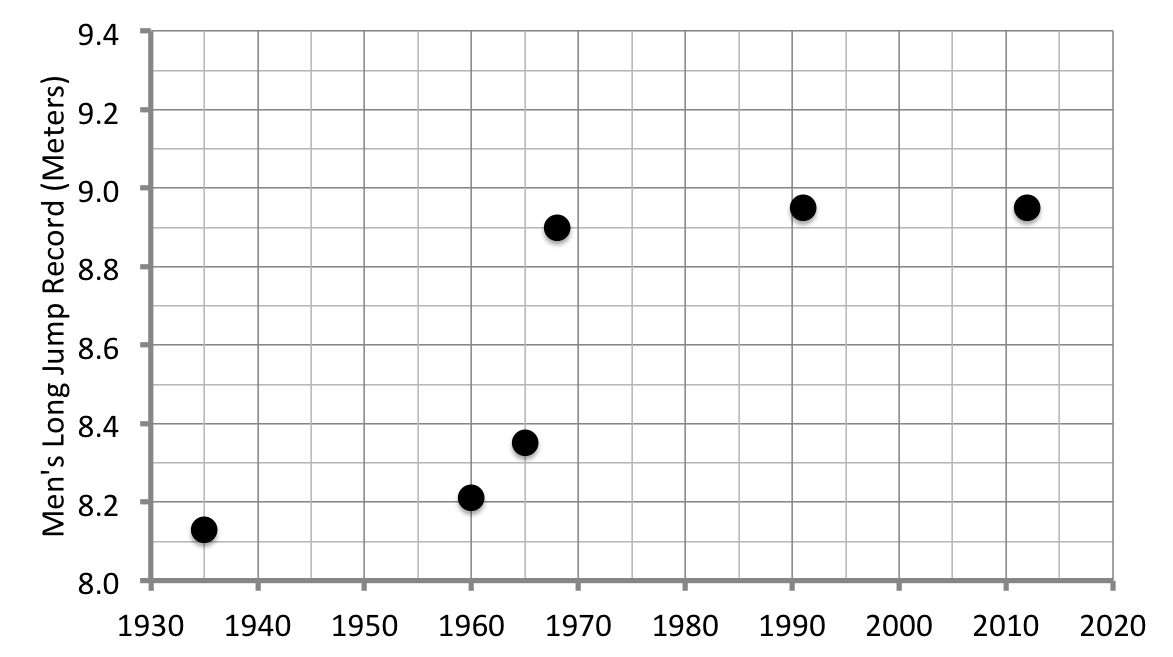
\includegraphics[width=\linewidth]{external/longjump.png}
\end{image}%
\begin{enumerate}[label=(\alph*),ref=\alph*]%
\item{}Draw in the line connecting the data from 1935 and 1991. Use it to predict the long jump record in 2020.%
\par\rule{\workspacestrutwidth}{0.75in}%
\item{}Draw in the line connecting the data from 1968 and 1991. Use it to predict the long jump record in 2020.%
\par\rule{\workspacestrutwidth}{0.75in}%
\item{}Which of your lines do you prefer, and why?%
\par\rule{\workspacestrutwidth}{0in}%
\end{enumerate}%
\end{divisionexercise}%
\clearpage
\begin{divisionexercise}{3}{}{}{rent-agreement-PE4B}%
Arjun just graduated from college but is living with his uncle for the summer to save money. They agreed that Arjun would do chores and some light renovations instead of paying rent. Arjun has been doing around 5 hours of work a week for the past 8 weeks, but still owes his uncle another 30 hours of work.%
\begin{enumerate}[label=(\alph*),ref=\alph*]%
\item{}What was the original agreement? That means, how many hours of work did Arjun originally promise his uncle?%
\par\rule{\workspacestrutwidth}{1.5in}%
\item{}Name the variables and write an equation relating them, assuming Arjun continues to do 5 hours a week of work.%
\par\rule{\workspacestrutwidth}{1.5in}%
\item{}How many more weeks will it take Arjun to finish the work he promised? Show how to solve the equation.%
\par\rule{\workspacestrutwidth}{1.5in}%
\end{enumerate}%
\end{divisionexercise}%
\clearpage
\begin{divisionexercise}{4}{}{}{zoning-PE4B}%
The local zoning commission is considering a plan to expand housing in the city, as measured in the number of residential units. But with more residential units come more shops, offices, schools, recreational facilities, churches, and other commercial property. Currently the city has 3,500 residential units and 1,575 acres of commercial property. If the proposal is passed and completed, the city will have a new total of 3,600 residential units and 1,620 acres of commercial property. You can assume this increase is linear.%
\begin{enumerate}[label=(\alph*),ref=\alph*]%
\item{}Name the variables and summarize the given information in a table.%
\par\rule{\workspacestrutwidth}{0.75in}%
\item{}How many new acres of commercial property are there for each new residential unit built?%
\par\rule{\workspacestrutwidth}{0.75in}%
\item{}Write an equation relating the variables. \emph{Hint: first find the intercept.}%
\par\rule{\workspacestrutwidth}{1.5in}%
\item{}If the city decides to limit the amount of land to 1,600 acres of commercial property, \emph{approximately} how many residential units can there be? Use successive approximation, displaying your guesses in a table.%
\par\rule{\workspacestrutwidth}{0.75in}%
\item{}Now answer the question \emph{exactly} by setting up and solving an inequality.%
\par\rule{\workspacestrutwidth}{0.75in}%
\end{enumerate}%
\end{divisionexercise}%
\end{exercises-subsection-numberless}
\end{sectionptx}
\end{chapterptx}
%
%
\typeout{************************************************}
\typeout{Chapter 5 A closer look at exponential equations}
\typeout{************************************************}
%
\begin{chapterptx}{Chapter}{A closer look at exponential equations}{}{A closer look at exponential equations}{}{}{ch-5-Closer_look_exponential}
\renewcommand*{\chaptername}{Chapter}
%
%
\typeout{************************************************}
\typeout{Section 5.1 Modeling with exponential equations - Practice exercises}
\typeout{************************************************}
%
\begin{sectionptx}{Section}{Modeling with exponential equations - Practice exercises}{}{Modeling with exponential equations - Practice exercises}{}{}{sec-5-1-Modeling_exponential_equations}
%
%
\typeout{************************************************}
\typeout{Exercises 5.1 Exercises}
\typeout{************************************************}
%
\begin{exercises-subsection-numberless}{Exercises}{Exercises}{}{Exercises}{}{}{ex-5-1-Modeling_exponential_equations}
\begin{divisionexercise}{1}{}{}{buenos-aires-modeling-exponential}%
The population of Buenos Aires, Argentina in 1950 was estimated at 5.0 million and expected to grow at 1.8\% each year. \begin{aside}{Aside}{}{buenos-aires-modeling-exponential-1-1-1}%
Source: Mongabay%
\end{aside}
%
\begin{enumerate}[label=(\alph*),ref=\alph*]%
\item{}Name the variables.%
\par\rule{\workspacestrutwidth}{0.75in}%
\item{}What is the annual growth factor?%
\par\rule{\workspacestrutwidth}{0.75in}%
\item{}Write an equation estimating the population of Buenos Aires over time.%
\par\rule{\workspacestrutwidth}{0.75in}%
\item{}Make a table of values showing the estimated population of Buenos Aires every 20th year from 1950 to 2030.%
\par\rule{\workspacestrutwidth}{2in}%
\item{}By approximately how many people has the population been increasing per year over each 20 year period? Add these numbers to your table. As expected, these numbers change because the rate of change is not constant.%
\item{}In 2000 the actual population of Buenos Aires was around 12.6 million and by 2010 it was around 15.2 million. How do these data compare to the estimates?%
\end{enumerate}%
\end{divisionexercise}%
\clearpage
\begin{divisionexercise}{2}{}{}{flu-dorm-modeling-exponential}%
A flu virus has been spreading through the college dormitories. \begin{aside}{Aside}{}{flu-dorm-modeling-exponential-1-1-1}%
(Story also appears in \hyperlink{flu-dorm-first-look-exponential}{{\xreffont 2.2.3}} and \hyperref[sec-5-5-Logistic_growth]{Section~{\xreffont\ref{sec-5-5-Logistic_growth}}})%
\end{aside}
 Initially 8 students were diagnosed with the flu, but that number has been growing 16\% per day. Earlier we found the equation%
\begin{equation*}
N=8 \ast1.16^T
\end{equation*}
where \(T\) is the time in days (since the first diagnosis) and \(N\) is the total number of students who had the flu.%
\begin{enumerate}[label=(\alph*),ref=\alph*]%
\item{}Use successive approximations to \emph{estimate} when the number of infected students reaches 100. Display your guesses in a table.%
\par
\begin{center}%
{\tabularfont%
\begin{tabular}{cccccccccc}\hrulethin
\multicolumn{1}{AcA}{{\bfseries{}\fillintext{3} (indep)}}&\multicolumn{1}{cA}{~~~~~ ~~~~~}&\multicolumn{1}{cA}{~~~~~ ~~~~~}&\multicolumn{1}{cA}{~~~~~ ~~~~~}&\multicolumn{1}{cA}{~~~~~ ~~~~~}&\multicolumn{1}{cA}{~~~~~ ~~~~~}&\multicolumn{1}{cA}{~~~~~ ~~~~~}&\multicolumn{1}{cA}{~~~~~ ~~~~~}&\multicolumn{1}{cA}{~~~~~ ~~~~~}&\multicolumn{1}{cA}{~~~~~ ~~~~~}\tabularnewline\hrulethin
\multicolumn{1}{AcA}{{\bfseries{}\fillintext{3} (dep)}}&\multicolumn{1}{cA}{}&\multicolumn{1}{cA}{}&\multicolumn{1}{cA}{}&\multicolumn{1}{cA}{}&\multicolumn{1}{cA}{}&\multicolumn{1}{cA}{}&\multicolumn{1}{cA}{}&\multicolumn{1}{cA}{}&\multicolumn{1}{cA}{}\tabularnewline\hrulethin
\multicolumn{1}{AcA}{{\bfseries{}hi \slash{} lo}}&\multicolumn{1}{cA}{}&\multicolumn{1}{cA}{}&\multicolumn{1}{cA}{}&\multicolumn{1}{cA}{}&\multicolumn{1}{cA}{}&\multicolumn{1}{cA}{}&\multicolumn{1}{cA}{}&\multicolumn{1}{cA}{}&\multicolumn{1}{cA}{}\tabularnewline\hrulethin
\end{tabular}
}%
\end{center}%
%
\par\rule{\workspacestrutwidth}{0.5in}%
\item{}Use the \hyperref[log-divides-formula]{Log-Divides Formula} to find \emph{exactly} when the number of infected students reaches 100.%
\par\rule{\workspacestrutwidth}{1.2in}%
\item{}There are 1,094 students currently living in the dorms. Suppose ultimately 250 students catch the flu. According to your equation, when would that happen? Show how to solve your equation.%
\par\rule{\workspacestrutwidth}{1.2in}%
\item{}It is not realistic to expect that everyone living in the dorms will catch the flu, but what does the equation say? Set up and solve an equation to find when all 1,094 students would have the flu. (Again, this is not realistic.)%
\par\rule{\workspacestrutwidth}{1in}%
\end{enumerate}%
\end{divisionexercise}%
\clearpage
\begin{divisionexercise}{3}{}{}{bunnies-modeling-exponential}%
Bunnies, bunnies, everywhere. \begin{aside}{Aside}{}{bunnies-modeling-exponential-1-1-1}%
(Story also appears in \hyperref[bunnies-prelude-scientific-notation]{{\xreffont 0.8.3}.{\xreffont\ref{bunnies-prelude-scientific-notation}}} and \hyperlink{bunnies-first-look-exponential}{{\xreffont 2.2.2}})%
\end{aside}
 Earlier we found the equation%
\begin{equation*}
B = 1{,}800 \ast 1.13^T
\end{equation*}
where \(B\) is the number of bunnies and \(T\) is the time in years since 2007.%
\begin{enumerate}[label=(\alph*),ref=\alph*]%
\item{}Make a table showing the number of bunnies in 2007, 2010, 2013, and 2020.%
\par\rule{\workspacestrutwidth}{0.75in}%
\item{}Draw a graph showing how the bunny population grew.%
\begin{image}{0.05}{0.9}{0.05}{}%

\includegraphics[width=\linewidth]{external/GraphPaper.jpg}
\end{image}%
\item{}\emph{Approximately} when will the population pass 5,000 bunnies? Guess from the graph. Then refine your answer using successive approximation.%
\par
\begin{center}%
{\tabularfont%
\begin{tabular}{cccccccccc}\hrulethin
\multicolumn{1}{AcA}{{\bfseries{}\fillintext{3} (indep)}}&\multicolumn{1}{cA}{~~~~~ ~~~~~}&\multicolumn{1}{cA}{~~~~~ ~~~~~}&\multicolumn{1}{cA}{~~~~~ ~~~~~}&\multicolumn{1}{cA}{~~~~~ ~~~~~}&\multicolumn{1}{cA}{~~~~~ ~~~~~}&\multicolumn{1}{cA}{~~~~~ ~~~~~}&\multicolumn{1}{cA}{~~~~~ ~~~~~}&\multicolumn{1}{cA}{~~~~~ ~~~~~}&\multicolumn{1}{cA}{~~~~~ ~~~~~}\tabularnewline\hrulethin
\multicolumn{1}{AcA}{{\bfseries{}\fillintext{3} (dep)}}&\multicolumn{1}{cA}{}&\multicolumn{1}{cA}{}&\multicolumn{1}{cA}{}&\multicolumn{1}{cA}{}&\multicolumn{1}{cA}{}&\multicolumn{1}{cA}{}&\multicolumn{1}{cA}{}&\multicolumn{1}{cA}{}&\multicolumn{1}{cA}{}\tabularnewline\hrulethin
\multicolumn{1}{AcA}{{\bfseries{}hi \slash{} lo}}&\multicolumn{1}{cA}{}&\multicolumn{1}{cA}{}&\multicolumn{1}{cA}{}&\multicolumn{1}{cA}{}&\multicolumn{1}{cA}{}&\multicolumn{1}{cA}{}&\multicolumn{1}{cA}{}&\multicolumn{1}{cA}{}&\multicolumn{1}{cA}{}\tabularnewline\hrulethin
\end{tabular}
}%
\end{center}%
%
\par\rule{\workspacestrutwidth}{0.25in}%
\item{}Solve your equation and check that you get the same answer.%
\end{enumerate}%
\end{divisionexercise}%
\clearpage
\begin{divisionexercise}{4}{}{}{greenhouse-co2-modeling-exponential}%
Carbon dioxide is a greenhouse gas in our atmosphere. Increasing carbon dioxide concentrations are related to global climate change. \begin{aside}{Aside}{}{greenhouse-co2-modeling-exponential-1-1-1}%
Source: Earth Systems Research Laboratory, NOAA%
\end{aside}
 In 1980, the carbon dioxide concentration was 338 ppm (parts per million). At that time it was assumed that carbon dioxide concentrations would increase 0.42\% per year.%
\begin{enumerate}[label=(\alph*),ref=\alph*]%
\item{}Name the variables including units.%
\par\rule{\workspacestrutwidth}{1.4in}%
\item{}Assuming the growth is exponential as predicted, write an equation that describes the increase in carbon dioxide concentrations.%
\par\rule{\workspacestrutwidth}{1.4in}%
\item{}The carbon dioxide concentration in 2008 was 385 ppm. Is that count higher or lower than predicted from your equation? Explain.%
\par\rule{\workspacestrutwidth}{1.4in}%
\item{}Does that mean that carbon dioxide increased at a higher or lower rate than 0.42\%? Explain.%
\par\rule{\workspacestrutwidth}{1.4in}%
\end{enumerate}%
\end{divisionexercise}%
\end{exercises-subsection-numberless}
\begin{conclusion}{When you're done \textellipsis{}}%
%
\begin{itemize}[label=\textbullet]
\item{}Check your solutions. Still confused? Work with a classmate, instructor, or tutor.%
\item{}Try the \alert{Do you know} questions. Not sure? Read the textbook and try again.%
\item{}Make a list of key ideas and processes to remember under \alert{Don't forget!}%
\item{}Do the textbook exercises and check your answers. Not sure if you are close enough? Compare answers with a classmate or ask your instructor or tutor.%
\item{}Getting the wrong answers or stuck? Re-read the section and try again. If you are still stuck, work with a classmate or go to your instructor's office hours or tutor hours.%
\item{}It is normal to find some parts of exercises difficult, but if most of them are a struggle, meet with your instructor or advisor about possible strategies or support services.%
\end{itemize}
%
\end{conclusion}%
\begin{conclusion}{Do you know \textellipsis{}}%
%
\begin{enumerate}[label={\Alph*.}]
\item{}What makes a function exponential?%
\item{}The template for an exponential equation? \emph{Ask your instructor if you need to remember the template or if it will be provided during the exam.}%
\item{}How to write an exponential equation given the starting amount and percent increase?%
\item{}Where the growth factor and starting amount appear in the template of an exponential equation?%
\item{}What the graph of an exponential function looks like?%
\item{}How to solve an exponential equation using the \hyperref[log-divides-formula]{Log-Divides Formula}?%
\par
\emph{Ask your instructor if you need to remember the \hyperref[log-divides-formula]{Log-Divides Formula} or if it will be provided during the exam.}%
\item{}How to calculate the rate of change of an exponential function?%
\item{}Why the rate of change of an exponential function is not constant?%
\end{enumerate}
%
\par
\alert{Don't forget!}%
\end{conclusion}%
\end{sectionptx}
%
%
\typeout{************************************************}
\typeout{Section 5.2 Exponential growth and decay - Practice exercises}
\typeout{************************************************}
%
\begin{sectionptx}{Section}{Exponential growth and decay - Practice exercises}{}{Exponential growth and decay - Practice exercises}{}{}{sec-5-2-Exp_growth_decay}
%
%
\typeout{************************************************}
\typeout{Exercises 5.2 Exercises}
\typeout{************************************************}
%
\begin{exercises-subsection-numberless}{Exercises}{Exercises}{}{Exercises}{}{}{ex-5-2-Exp_growth_decay}
\begin{divisionexercise}{1}{}{}{fiber-optic-growth-decay}%
A signal is sent down a fiber optic cable. \begin{aside}{Aside}{}{fiber-optic-growth-decay-1-1-1}%
(Story also appears in \hyperref[fiber-optic-prelude-scientific-notation]{{\xreffont 0.8.3}.{\xreffont\ref{fiber-optic-prelude-scientific-notation}}} and \hyperlink{fiber-optic-powers-roots}{{\xreffont 0.6.3}})%
\end{aside}
 Its strength decreases by 2\% each mile it travels. (Say it was one unit strong to start.)%
\begin{enumerate}[label=(\alph*),ref=\alph*]%
\item{}Name the variables, including units.%
\par\rule{\workspacestrutwidth}{1in}%
\item{}Make a table showing the strength of the signal over the first five miles.%
\par\rule{\workspacestrutwidth}{1.75in}%
\item{}Write an equation relating the variables.%
\par\rule{\workspacestrutwidth}{1.5in}%
\item{}The signal will need a \terminology{booster} (something to make the signal stronger again) when it has fallen to under 0.75 units. How far along the cable should the booster be placed? Set up and solve an equation.%
\par\rule{\workspacestrutwidth}{1.5in}%
\item{}\emph{The problem continues \textellipsis{}}%
\par
What is the half-life (or should we say half-distance) of a signal? That means, how far can it travel without dropping below 0.5? (That will not actually happen because we would boost the signal.) Again, set up and solve an equation.%
\par\rule{\workspacestrutwidth}{3in}%
\item{}Draw a graph illustrating the relationship.%
\begin{image}{0.05}{0.9}{0.05}{}%

\includegraphics[width=\linewidth]{external/GraphPaper.jpg}
\end{image}%
\item{}Indicate the points on your graph where you can check your answers to parts (c) and (d).%
\end{enumerate}%
\end{divisionexercise}%
\clearpage
\begin{divisionexercise}{2}{}{}{cellphone-doubling-growth-decay}%
A recent news report stated that cell phone usage is growing exponentially in developing countries. In one small country, 50,000 people owned a cell phone in the year 2000. It was estimated that usage would increase at 1.4\% percent per year.%
\begin{enumerate}[label=(\alph*),ref=\alph*]%
\item{}Name the variables including units.%
\par\rule{\workspacestrutwidth}{0.75in}%
\item{}Assuming the growth is exponential, write an equation for the function.%
\par\rule{\workspacestrutwidth}{0.75in}%
\item{}At this rate, how many years would it take for the number of people owning a cell phone to double? That is called the \terminology{doubling time}. Show how to set up and solve an equation to find the answer.%
\par\rule{\workspacestrutwidth}{2in}%
\item{}In 2011, about 682,000 people owned a cellphone. Is that count higher or lower than predicted from your equation? Explain.%
\par\rule{\workspacestrutwidth}{0.75in}%
\item{}Based on the 2011 data, would you say that cell phone usage was growing slower or faster than 1.4\%?%
\par\rule{\workspacestrutwidth}{0.75in}%
\end{enumerate}%
\end{divisionexercise}%
\clearpage
\begin{divisionexercise}{3}{}{}{heart-attack-growth-decay}%
If a person has a heart attack and their heart stops beating, the amount of time it takes paramedics to restart their heart with a defibrillator is critical. Each minute that passes decreases the person's chance of survival by 10\%. \begin{aside}{Aside}{}{heart-attack-growth-decay-1-1-1}%
Source: American Red Cross%
\end{aside}
 Assume that this statement means the decrease is exponential and that the survival rate is 100\% if the defibrillator is used immediately.%
\begin{enumerate}[label=(\alph*),ref=\alph*]%
\item{}Name the variables, including units, and write an equation.%
\par\rule{\workspacestrutwidth}{1in}%
\item{}If it takes the paramedics 2 minutes to use the defibrillator, what is the person's chance of survival?%
\par\rule{\workspacestrutwidth}{1in}%
\item{}Use successive approximation to \emph{estimate} to the nearest minute when the survival rate drops below 50\%. Display your guesses in a table.%
\par
\begin{center}%
{\tabularfont%
\begin{tabular}{cccccccccc}\hrulethin
\multicolumn{1}{AcA}{{\bfseries{}\fillintext{3} (indep)}}&\multicolumn{1}{cA}{~~~~~ ~~~~~}&\multicolumn{1}{cA}{~~~~~ ~~~~~}&\multicolumn{1}{cA}{~~~~~ ~~~~~}&\multicolumn{1}{cA}{~~~~~ ~~~~~}&\multicolumn{1}{cA}{~~~~~ ~~~~~}&\multicolumn{1}{cA}{~~~~~ ~~~~~}&\multicolumn{1}{cA}{~~~~~ ~~~~~}&\multicolumn{1}{cA}{~~~~~ ~~~~~}&\multicolumn{1}{cA}{~~~~~ ~~~~~}\tabularnewline\hrulethin
\multicolumn{1}{AcA}{{\bfseries{}\fillintext{3} (dep)}}&\multicolumn{1}{cA}{}&\multicolumn{1}{cA}{}&\multicolumn{1}{cA}{}&\multicolumn{1}{cA}{}&\multicolumn{1}{cA}{}&\multicolumn{1}{cA}{}&\multicolumn{1}{cA}{}&\multicolumn{1}{cA}{}&\multicolumn{1}{cA}{}\tabularnewline\hrulethin
\multicolumn{1}{AcA}{{\bfseries{}hi \slash{} lo}}&\multicolumn{1}{cA}{}&\multicolumn{1}{cA}{}&\multicolumn{1}{cA}{}&\multicolumn{1}{cA}{}&\multicolumn{1}{cA}{}&\multicolumn{1}{cA}{}&\multicolumn{1}{cA}{}&\multicolumn{1}{cA}{}&\multicolumn{1}{cA}{}\tabularnewline\hrulethin
\end{tabular}
}%
\end{center}%
%
\par\rule{\workspacestrutwidth}{1in}%
\item{}Solve your equation to find \emph{exactly} when the survival rate drops below 50\%.%
\end{enumerate}%
\end{divisionexercise}%
\clearpage
\begin{divisionexercise}{4}{}{}{ten-likes-growth-decay}%
You and two buddies each invite 10 people to ``like'' your online group. Suppose everyone accepts and then they each invite 10 people. And then everyone accepts and they each invite 10 people. And so on. Of course, there is likely to be substantial overlap, but for the moment pretend that there is not any overlap.%
\begin{enumerate}[label=(\alph*),ref=\alph*]%
\item{}There are 3 friends to start. In the first round they each invite 10 friends, so a total of 30 new people ``like'' your online group in the first round. How many new people ``like'' your group in the second round? The third?%
\par\rule{\workspacestrutwidth}{0.75in}%
\item{}Name the variables and write an equation showing how the number of new people increases in each round. Think of the original 3 friends as round 0.%
\par\rule{\workspacestrutwidth}{1.5in}%
\item{}Make a table showing this information. Continue your table to include the number of new people who ``like'' your group in the fourth and fifth rounds.%
\par\rule{\workspacestrutwidth}{0.75in}%
\item{}What is the \emph{total} number of people who ``like'' your online group after five rounds? \emph{Hint: add}%
\par\rule{\workspacestrutwidth}{0.75in}%
\item{}Comment on why our assumption is unrealistic.%
\par\rule{\workspacestrutwidth}{1in}%
\end{enumerate}%
\end{divisionexercise}%
\end{exercises-subsection-numberless}
\begin{conclusion}{When you're done \textellipsis{}}%
%
\begin{itemize}[label=\textbullet]
\item{}Check your solutions. Still confused? Work with a classmate, instructor, or tutor.%
\item{}Try the \alert{Do you know} questions. Not sure? Read the textbook and try again.%
\item{}Make a list of key ideas and processes to remember under \alert{Don't forget!}%
\item{}Do the textbook exercises and check your answers. Not sure if you are close enough? Compare answers with a classmate or ask your instructor or tutor.%
\item{}Getting the wrong answers or stuck? Re-read the section and try again. If you are still stuck, work with a classmate or go to your instructor's office hours or tutor hours.%
\item{}It is normal to find some parts of exercises difficult, but if most of them are a struggle, meet with your instructor or advisor about possible strategies or support services.%
\end{itemize}
%
\end{conclusion}%
\begin{conclusion}{Do you know \textellipsis{}}%
%
\begin{enumerate}[label={\Alph*.}]
\item{}How to write an exponential equation given the starting amount and percent decrease?%
\item{}What ``half-life'' means?%
\item{}What ``doubling time'' means?%
\item{}What the graph of exponential growth and exponential decay look like?%
\item{}Why the rate of change for exponential decay is negative?%
\end{enumerate}
%
\par
\alert{Don't forget!}%
\end{conclusion}%
\end{sectionptx}
%
%
\typeout{************************************************}
\typeout{Section 5.3 Growth factors - Practice exercises}
\typeout{************************************************}
%
\begin{sectionptx}{Section}{Growth factors - Practice exercises}{}{Growth factors - Practice exercises}{}{}{sec-5-3-Growth_factor}
%
%
\typeout{************************************************}
\typeout{Exercises 5.3 Exercises}
\typeout{************************************************}
%
\begin{exercises-subsection-numberless}{Exercises}{Exercises}{}{Exercises}{}{}{ex-5-3-Growth_factor}
\begin{assemblage}{Assemblage}{Percent Change Formula}{percent-change-formula}%
%
\begin{itemize}[label=\textbullet]
\item{}If a quantity changes by a percentage corresponding to growth rate \(r\), then the growth factor is%
\begin{equation*}
\displaystyle g=1+r
\end{equation*}
%
\item{}If the growth factor is \(g\), then the growth rate is%
\begin{equation*}
r = g-1
\end{equation*}
%
\end{itemize}
%
\end{assemblage}
 \begin{assemblage}{Assemblage}{Growth Factor Formula}{growth-factor-formula}%
If a quantity is growing (or decaying) exponentially, then the growth (or decay) factor is%
\begin{equation*}
\displaystyle g = \sqrt[t]{\frac{a}{s}}
\end{equation*}
where \(s\) is the starting amount and \(a\) is the amount after \(t\) time periods.%
\end{assemblage}
\clearpage
\begin{divisionexercise}{1}{}{}{grandfather-bonds-growth-factor}%
In 1962, my grandfather had savings bonds that matured to \textdollar{}200. \begin{aside}{Aside}{}{grandfather-bonds-growth-factor-1-1-1}%
(Story also appears in \hyperref[sec-1-1-Variables_and_functions]{{\xreffont\ref{sec-1-1-Variables_and_functions}}} Exercises and \hyperlink{grandfather-bonds-growth-factor}{{\xreffont 5.3.1}})%
\end{aside}
 He gave those to my mother to keep for me. These bonds have continued to earn interest at a fixed, guaranteed rate so I have yet to cash them in. The table lists the value at various times since then.%
 \begin{center}%
{\tabularfont%
\begin{tabular}{lllllll}\hrulethin
\multicolumn{1}{AcA}{year}&\multicolumn{1}{cA}{1962}&\multicolumn{1}{cA}{1970}&\multicolumn{1}{cA}{1980}&\multicolumn{1}{cA}{1990}&\multicolumn{1}{cA}{2000}&\multicolumn{1}{cA}{2010}\tabularnewline\hrulethin
\multicolumn{1}{AcA}{years since 1962}&\multicolumn{1}{cA}{0}&\multicolumn{1}{cA}{8}&\multicolumn{1}{cA}{18}&\multicolumn{1}{cA}{28}&\multicolumn{1}{cA}{38}&\multicolumn{1}{cA}{48}\tabularnewline\hrulethin
\multicolumn{1}{AcA}{value}&\multicolumn{1}{cA}{200.00}&\multicolumn{1}{cA}{318.77}&\multicolumn{1}{cA}{570.87}&\multicolumn{1}{cA}{1,022.34}&\multicolumn{1}{cA}{1,830.85}&\multicolumn{1}{cA}{3,278.77}\tabularnewline\hrulethin
\end{tabular}
}%
\end{center}%
\begin{enumerate}[label=(\alph*),ref=\alph*]%
\item{}Use the \hyperref[growth-factor-formula]{Growth Factor Formula} to find the annual growth factor for the time period from 1962 to 1970.%
\par\rule{\workspacestrutwidth}{0.7in}%
\item{}Repeat for 1970 to 1980.%
\par\rule{\workspacestrutwidth}{0.7in}%
\item{}What do you notice? What in the story told you that would happen?%
\par\rule{\workspacestrutwidth}{0.7in}%
\item{}What is the corresponding interest rate?%
\par\rule{\workspacestrutwidth}{0.7in}%
\item{}Write an equation for the value of bonds over time.%
\par\rule{\workspacestrutwidth}{0.7in}%
\item{}Use your equation to check the information for 1990, 2000, and 2010.%
\par\rule{\workspacestrutwidth}{0.5in}%
\item{}\emph{The problem continues \textellipsis{}}%
\par
In what year will the bond be worth over \textdollar{}5,000? Set up and solve an equation to decide.%
\par\rule{\workspacestrutwidth}{3in}%
\item{}Draw a graph using the data in the table, but not your answer to part (g). Include another year that is later than your answer to part (g).%
\begin{image}{0.05}{0.9}{0.05}{}%

\includegraphics[width=\linewidth]{external/GraphPaper.jpg}
\end{image}%
\par\rule{\workspacestrutwidth}{0in}%
\item{}Does your answer to part (g) agree with your graph? If not, fix your work.%
\par\rule{\workspacestrutwidth}{0in}%
\end{enumerate}%
\end{divisionexercise}%
\clearpage
\begin{divisionexercise}{2}{}{}{carbon-14-growth-factor}%
Have you read news stories about archaeological digs where a specimen (like a bone) is found that dates back thousands of years? How do scientists know how old something is? One method uses the radioactive decay of carbon. \begin{aside}{Aside}{}{carbon-14-growth-factor-1-1-1}%
Source: Wikipedia (Radiocarbon Dating)%
\end{aside}
 After an animal dies the carbon-14 in its body very slowly decays. By comparing how much carbon-14 remains in the bone to how much carbon-14 should have been in the bone when the animal was alive, scientist can estimate how long the animal has been dead. Clever, huh? Actually, it is so clever that Willard Libby won the Nobel Prize in Chemistry for it. The key information to know is that the \terminology{half-life} of carbon-14 (the amount of time it takes for half of the original amount of carbon-14 to decay) is about 5,730 years. For this problem, suppose a bone were found that should have contained 300 milligrams of carbon-14 when the animal was alive.%
\begin{enumerate}[label=(\alph*),ref=\alph*]%
\item{}Find the annual ``growth'' factor. Keep at least six digits after the decimal place for your calculations.%
\par\smallskip%
\noindent\textbf{\blocktitlefont Hint}.\hypertarget{carbon-14-growth-factor-2-2}{}\quad{}If the bone started off with 300 mg of carbon-14, how much carbon-14 would be left after 5,730 years?%
\par\rule{\workspacestrutwidth}{1in}%
\item{}Name the variables and write an equation describing the dependence.%
\par\rule{\workspacestrutwidth}{1in}%
\item{}How many milligrams of carbon-14 should remain in this bone after 1,000 years? After 10,000 years? After 100,000 years?%
\par\rule{\workspacestrutwidth}{1in}%
\item{}How many milligrams of carbon-14 should remain in this bone after 1 million years? Explain the ``scientific notation'' answer your calculator gives you.%
\par\rule{\workspacestrutwidth}{0.75in}%
\item{}\emph{The problem continues \textellipsis{}}%
\par
Draw a graph that shows up to 10,000 years.%
\begin{image}{0.05}{0.9}{0.05}{}%

\includegraphics[width=\linewidth]{external/GraphPaper.jpg}
\end{image}%
\par\rule{\workspacestrutwidth}{0in}%
\item{}If the bone is determined to have 100 milligrams of carbon-14, \emph{approximately} how long ago did it die? Start by \emph{estimating} the answer from your graph. Then revise your estimate using successive approximation. Display your guesses in a table.%
\par\rule{\workspacestrutwidth}{1in}%
\item{}Solve the equation exactly.%
\par\rule{\workspacestrutwidth}{1in}%
\end{enumerate}%
\end{divisionexercise}%
\clearpage
\begin{divisionexercise}{3}{}{}{find-growth-factor}%
For each story, find the annual growth factor \(g\) and annual growth rate \(r\) as a percent.%
 \par
\emph{Hint: First decide if you can use the \hyperref[percent-change-formula]{Percent Change Formula} or if you will need to use the \hyperref[growth-factor-formula]{Growth Factor Formula}. Don't forget to include the negative sign for decay rates.}%
\begin{enumerate}[label=(\alph*),ref=\alph*]%
\item{}Donations to the food shelf have increased 35\% per year for the past few years.%
\begin{sidebyside}{3}{0}{0}{0}%
\begin{sbspanel}{0.75}%
%
\end{sbspanel}%
\begin{sbspanel}{0.1}%
\par
%
\begin{equation*}
g=
\end{equation*}
%
\begin{equation*}
r =
\end{equation*}
%
\end{sbspanel}%
\begin{sbspanel}{0.15}%
\par
%
\end{sbspanel}%
\end{sidebyside}%
\par\rule{\workspacestrutwidth}{1.75cm}%
\item{}People picking up food at the food shelf has increased exponentially too, from 120 per week in 2005 to 630 per week in 2011.%
\begin{sidebyside}{3}{0}{0}{0}%
\begin{sbspanel}{0.75}%
%
\end{sbspanel}%
\begin{sbspanel}{0.1}%
\par
%
\begin{equation*}
g=
\end{equation*}
%
\begin{equation*}
r =
\end{equation*}
%
\end{sbspanel}%
\begin{sbspanel}{0.15}%
\par
%
\end{sbspanel}%
\end{sidebyside}%
\par\rule{\workspacestrutwidth}{1.75cm}%
\item{}The crime rate has dropped 3\% each year recently.%
\begin{sidebyside}{3}{0}{0}{0}%
\begin{sbspanel}{0.75}%
%
\end{sbspanel}%
\begin{sbspanel}{0.1}%
\par
%
\begin{equation*}
g=
\end{equation*}
%
\begin{equation*}
r =
\end{equation*}
%
\end{sbspanel}%
\begin{sbspanel}{0.15}%
\par
%
\end{sbspanel}%
\end{sidebyside}%
\par\rule{\workspacestrutwidth}{1.75cm}%
\item{}The new stop sign has decreased accidents exponentially, from 40 in 2008 to 17 in 2013.%
\begin{sidebyside}{3}{0}{0}{0}%
\begin{sbspanel}{0.75}%
%
\end{sbspanel}%
\begin{sbspanel}{0.1}%
\par
%
\begin{equation*}
g=
\end{equation*}
%
\begin{equation*}
r =
\end{equation*}
%
\end{sbspanel}%
\begin{sbspanel}{0.15}%
\par
%
\end{sbspanel}%
\end{sidebyside}%
\par\rule{\workspacestrutwidth}{1cm}%
\item{}\emph{The problem continues \textellipsis{}}%
\par
The creeping vine taking over Fiona's lawn will double in area each year.%
\begin{sidebyside}{3}{0}{0}{0}%
\begin{sbspanel}{0.75}%
%
\end{sbspanel}%
\begin{sbspanel}{0.1}%
\par
%
\begin{equation*}
g=
\end{equation*}
%
\begin{equation*}
r =
\end{equation*}
%
\end{sbspanel}%
\begin{sbspanel}{0.15}%
\par
%
\end{sbspanel}%
\end{sidebyside}%
\par\rule{\workspacestrutwidth}{1.75cm}%
\item{}Attendance at parent volunteer night has doubled every 3 years.%
\begin{sidebyside}{3}{0}{0}{0}%
\begin{sbspanel}{0.75}%
%
\end{sbspanel}%
\begin{sbspanel}{0.1}%
\par
%
\begin{equation*}
g=
\end{equation*}
%
\begin{equation*}
r =
\end{equation*}
%
\end{sbspanel}%
\begin{sbspanel}{0.15}%
\par
%
\end{sbspanel}%
\end{sidebyside}%
\par\rule{\workspacestrutwidth}{1.75cm}%
\item{}The number of people addicted to prescription drugs was estimated to have tripled in the past 5 years. Assume the number is increasing exponentially.%
\begin{sidebyside}{3}{0}{0}{0}%
\begin{sbspanel}{0.75}%
%
\end{sbspanel}%
\begin{sbspanel}{0.1}%
\par
%
\begin{equation*}
g=
\end{equation*}
%
\begin{equation*}
r =
\end{equation*}
%
\end{sbspanel}%
\begin{sbspanel}{0.15}%
\par
%
\end{sbspanel}%
\end{sidebyside}%
\par\rule{\workspacestrutwidth}{1.75cm}%
\item{}The number of high school students arrested for driving under the influence is half what it was 5 years ago. Assume the number is falling exponentially.%
\begin{sidebyside}{3}{0}{0}{0}%
\begin{sbspanel}{0.75}%
%
\end{sbspanel}%
\begin{sbspanel}{0.1}%
\par
%
\begin{equation*}
g=
\end{equation*}
%
\begin{equation*}
r =
\end{equation*}
%
\end{sbspanel}%
\begin{sbspanel}{0.15}%
\par
%
\end{sbspanel}%
\end{sidebyside}%
\par\rule{\workspacestrutwidth}{1.75cm}%
\end{enumerate}%
\end{divisionexercise}%
\clearpage
\begin{divisionexercise}{4}{}{}{ex-5-3-Growth_factor-5-1}%
For each equation, find the growth rate and state its units. For example, something might ``grow 2\% per year'' while something else might ``drop 7\% per hour''.%
\begin{enumerate}[label=(\alph*),ref=\alph*]%
\item\label{reality-tv-growth-factor}The number of households watching reality television \(R\) (in millions) was estimated by the equation \begin{aside}{Aside}{}{reality-tv-growth-factor-1-1-2}%
(Story also appears in \hyperref[sec-5-1-Modeling_exponential_equations]{{\xreffont\ref{sec-5-1-Modeling_exponential_equations}}} Exercises)%
\end{aside}
%
\begin{equation*}
R=2.5 \ast 1.072^T
\end{equation*}
where \(T\) is the time in years since 1990.%
\par\rule{\workspacestrutwidth}{1.5in}%
\item\label{chlorine-pool-growth-factor}Chlorine is often used to disinfect water in swimming pools, but the concentration of chlorine \(C\) (in ppm) drops as the swimming pool is used for \(T\) hours according to the equation \begin{aside}{Aside}{}{chlorine-pool-growth-factor-1-1-3}%
(Story also appears in \hyperlink{chlorine-pool-solving-exponential}{{\xreffont 3.4.2}})%
\end{aside}
%
\begin{equation*}
C = 2.5 \ast 0.975^T
\end{equation*}
%
\par\rule{\workspacestrutwidth}{1.5in}%
\item\label{drawing-game-growth-factor}The number of players of a wildly popular mobile app drawing game has been growing exponentially according to the equation \begin{aside}{Aside}{}{drawing-game-growth-factor-1-1-1}%
(Story also appears in \hyperref[sec-5-1-Modeling_exponential_equations]{{\xreffont\ref{sec-5-1-Modeling_exponential_equations}}} Exercises)%
\end{aside}
 where \(N\) is the number of players (in millions) and \(T\) is the time in weeks since people started playing the game.%
\begin{equation*}
N = 2 \ast 1.57^W
\end{equation*}
%
\par\rule{\workspacestrutwidth}{1.5in}%
\end{enumerate}%
\end{divisionexercise}%
\end{exercises-subsection-numberless}
\begin{conclusion}{When you're done \textellipsis{}}%
%
\begin{itemize}[label=\textbullet]
\item{}Check your solutions. Still confused? Work with a classmate, instructor, or tutor.%
\item{}Try the \alert{Do you know} questions. Not sure? Read the textbook and try again.%
\item{}Make a list of key ideas and processes to remember under \alert{Don't forget!}%
\item{}Do the textbook exercises and check your answers. Not sure if you are close enough? Compare answers with a classmate or ask your instructor or tutor.%
\item{}Getting the wrong answers or stuck? Re-read the section and try again. If you are still stuck, work with a classmate or go to your instructor's office hours or tutor hours.%
\item{}It is normal to find some parts of exercises difficult, but if most of them are a struggle, meet with your instructor or advisor about possible strategies or support services.%
\end{itemize}
%
\end{conclusion}%
\begin{conclusion}{Do you know \textellipsis{}}%
%
\begin{enumerate}[label={\Alph*.}]
\item{}How to find the growth\slash{}decay factor given the starting amount and another point of information?%
\item{}How to find the growth\slash{}decay factor given the doubling time or half-life?%
\item{}When we use the \hyperref[percent-change-formula]{Percent Change Formula}, and when we use the \hyperref[growth-factor-formula]{Growth Factor Formula} instead? \emph{Ask your instructor if you need to remember the \hyperref[percent-change-formula]{Percent Change Formula} and \hyperref[growth-factor-formula]{Growth Factor Formula} or if they will be provided during the exam.}%
\item{}How to evaluate the \hyperref[percent-change-formula]{Percent Change Formula} and \hyperref[growth-factor-formula]{Growth Factor Formula} using your calcuator?%
\item{}How to read the starting amount and percent increase\slash{}decrease from the equation?%
\end{enumerate}
%
\par
\alert{Don't forget!}%
\end{conclusion}%
\end{sectionptx}
%
%
\typeout{************************************************}
\typeout{Section 5.4 Linear vs. exponential models - Practice exercises}
\typeout{************************************************}
%
\begin{sectionptx}{Section}{Linear vs. exponential models - Practice exercises}{}{Linear vs. exponential models - Practice exercises}{}{}{sec-5-4-Linear_vs_exponential}
%
%
\typeout{************************************************}
\typeout{Exercises 5.4 Exercises}
\typeout{************************************************}
%
\begin{exercises-subsection-numberless}{Exercises}{Exercises}{}{Exercises}{}{}{ex-5-4-Linear_vs_exponential}
\begin{assemblage}{Assemblage}{Linear Equation Template}{linear-eq-template}%
%
\begin{equation*}
\text{dep} = \text{start} + \text{slope} \ast \text{indep}
\end{equation*}
%
\end{assemblage}
 \begin{assemblage}{Assemblage}{Rate of Change Formula}{rate-of-change}%
%
\begin{equation*}
\text{rate of change } = \frac{\text{change dep}}{\text{change indep}} = \frac{\text{1st dep - 2nd dep}}{\text{1st indep - 2nd indep}}
\end{equation*}
%
\end{assemblage}
 \begin{assemblage}{Assemblage}{Exponential Equation Template}{exp-eqn-template}%
%
\begin{equation*}
\text{dep} = \text{start} \ast \text{growth factor} ^ {\text{indep}}
\end{equation*}
%
\end{assemblage}
 \begin{assemblage}{Assemblage}{Growth Factor Formula}{ex-5-4-Linear_vs_exponential-1-1-4}%
If a quantity is growing (or decaying) exponentially, then the growth (or decay) factor is%
\begin{equation*}
\displaystyle g = \sqrt[t]{\frac{a}{s}}
\end{equation*}
where \(s\) is the starting amount and \(a\) is the amount after \(t\) time periods.%
\end{assemblage}
 \begin{assemblage}{Assemblage}{Percent Change Formula}{ex-5-4-Linear_vs_exponential-1-1-5}%
%
\begin{itemize}[label=\textbullet]
\item{}If a quantity changes by a percentage corresponding to growth rate \(r\), then the growth factor is%
\begin{equation*}
\displaystyle g=1+r
\end{equation*}
%
\item{}If the growth factor is \(g\), then the growth rate is%
\begin{equation*}
r = g-1
\end{equation*}
%
\end{itemize}
%
\end{assemblage}
\clearpage
\begin{divisionexercise}{1}{}{}{parents-house-linear-exponential}%
My parents bought the house I grew up in for \textdollar{}35,000 and sold it 40 years later for \textdollar{}342,000. True story. (It was before the housing bubble burst.)%
 \par
\alert{First, assume the value of the house increased exponentially.}%
\begin{enumerate}[label=(\alph*),ref=\alph*]%
\item{}Calculate the annual growth factor using the \hyperref[growth-factor-formula]{Growth Factor Formula}.%
\par\rule{\workspacestrutwidth}{1.75in}%
\item{}In this model, by what percentage did the house value increase each year? \emph{Hint: use the \hyperref[percent-change-formula]{Percent Change Formula}.}%
\par\rule{\workspacestrutwidth}{0.75in}%
\item{}Write an exponential equation showing how the value of the house increased. Don't forget to name the variables, including units. \emph{Hint: use the \hyperref[exp-eqn-template]{Exponential Equation Template}.}%
\par\rule{\workspacestrutwidth}{2.5in}%
\item{}Check that your equation gives the correct sold value.%
\par\rule{\workspacestrutwidth}{0.5in}%
\item{}\emph{The problem continues \textellipsis{}}%
\par
\alert{Next, assume the value of the house increased linearly instead.}%
\par
In this model, by what fixed amount did the house value increase each year? \emph{Hint: calculate the slope using the \hyperref[rate-of-change]{Rate of Change Formula}.}%
\par\rule{\workspacestrutwidth}{2.5in}%
\item{}Using the same variables, write a linear equation showing how the value of the house increased. \emph{Hint: use the \hyperref[linear-eq-template]{Linear Equation Template}.}%
\par\rule{\workspacestrutwidth}{2in}%
\item{}Check that your equation gives the correct sold value.%
\end{enumerate}%
\end{divisionexercise}%
\clearpage
\begin{divisionexercise}{2}{}{}{manufacturing-jobs-linear-exponential}%
The number of manufacturing jobs in the state has been declining for decades. In 1970, there were 1.2 million such jobs in the state but by 2010 there were only 0.6 million such jobs. Write \(J\) for the number of manufacturing jobs (in millions) and \(T\) for time in years since 1970.%
 \par
\alert{First, assume the number of jobs decreased linearly.}%
\begin{enumerate}[label=(\alph*),ref=\alph*]%
\item{}Calculate the slope.%
\par\rule{\workspacestrutwidth}{1in}%
\item{}Write a linear equation showing how the number of jobs declined.%
\par\rule{\workspacestrutwidth}{1in}%
\item{}Check that your equation gives the correct value for 2010.%
\par\rule{\workspacestrutwidth}{0.25in}%
\item{}\alert{Next, assume the number of jobs decreased exponentially instead.}%
\par
Calculate the growth factor.%
\par\rule{\workspacestrutwidth}{1in}%
\item{}Write an exponential equation showing how the number of jobs declined.%
\par\rule{\workspacestrutwidth}{1in}%
\item{}Check that your equation gives the correct value for 2010.%
\par\rule{\workspacestrutwidth}{0.25in}%
\item{}\emph{The problem continues \textellipsis{}}%
\par
\alert{Now, compare the models.}%
\par
Complete the table of values.%
\begin{center}%
{\tabularfont%
\begin{tabular}{llllll}\hrulethin
\multicolumn{1}{AcA}{year}&\multicolumn{1}{cA}{1970}&\multicolumn{1}{cA}{1990}&\multicolumn{1}{cA}{2010}&\multicolumn{1}{cA}{2020}&\multicolumn{1}{cA}{2030}\tabularnewline\hrulethin
\multicolumn{1}{AcA}{\(T\)}&\multicolumn{1}{cA}{0}&\multicolumn{1}{cA}{20}&\multicolumn{1}{cA}{40}&\multicolumn{1}{cA}{50}&\multicolumn{1}{cA}{60}\tabularnewline\hrulethin
\multicolumn{1}{AcA}{\(J\) (if linear)}&\multicolumn{1}{cA}{\(\fillinmath{\begin{array}{cc}xxxx\\xxxx\end{array}}\)}&\multicolumn{1}{cA}{\(\fillinmath{\begin{array}{cc}xxxx\\xxxx\end{array}}\)}&\multicolumn{1}{cA}{\(\fillinmath{\begin{array}{cc}xxxx\\xxxx\end{array}}\)}&\multicolumn{1}{cA}{\(\fillinmath{\begin{array}{cc}xxxx\\xxxx\end{array}}\)}&\multicolumn{1}{cA}{\(\fillinmath{\begin{array}{cc}xxxx\\xxxx\end{array}}\)}\tabularnewline\hrulethin
\multicolumn{1}{AcA}{\(J\) (if exponential)}&\multicolumn{1}{cA}{\(\fillinmath{\begin{array}{cc}xxxx\\xxxx\end{array}}\)}&\multicolumn{1}{cA}{\(\fillinmath{\begin{array}{cc}xxxx\\xxxx\end{array}}\)}&\multicolumn{1}{cA}{\(\fillinmath{\begin{array}{cc}xxxx\\xxxx\end{array}}\)}&\multicolumn{1}{cA}{\(\fillinmath{\begin{array}{cc}xxxx\\xxxx\end{array}}\)}&\multicolumn{1}{cA}{\(\fillinmath{\begin{array}{cc}xxxx\\xxxx\end{array}}\)}\tabularnewline\hrulethin
\end{tabular}
}%
\end{center}%
\item{}Draw a graph showing both models.%
\begin{image}{0.05}{0.9}{0.05}{}%

\includegraphics[width=\linewidth]{external/GraphPaper.jpg}
\end{image}%
\item{}Which model has better news for 2030?%
\end{enumerate}%
\end{divisionexercise}%
\clearpage
\begin{divisionexercise}{3}{}{}{angry-birds-linear-exponential}%
In December 2010, a popular mobile app game featuring animated birds launched from slingshots had 50 million downloads. Five months later (May 2011), the game had 200 million downloads. Let \(D\) denote the number of downloads of the game (in millions) and \(T\) the time in months since December 2010.%
\begin{enumerate}[label=(\alph*),ref=\alph*]%
\item{}Suppose that the number of downloads have been increasing at a \emph{constant rate each month}. What type of equation is suggested here? Write that equation and use it to estimate the number of downloads in November 2011 (when T = 11).%
\par\rule{\workspacestrutwidth}{2.5in}%
\item{}Suppose that the number of downloads have been increasing at a \emph{fixed percentage each month}. What type of equation is suggested here? Write that equation and use it to estimate the number of downloads in November 2011 (when T = 11).%
\par\rule{\workspacestrutwidth}{2.5in}%
\item{}Which of these two models do you think is more sensible, and why?%
\par\rule{\workspacestrutwidth}{0in}%
\end{enumerate}%
\end{divisionexercise}%
\clearpage
\begin{divisionexercise}{4}{}{}{bus-fares-linear-exponential}%
Bus fares are up to \textdollar{}2.25 per ride during rush hour. Two different plans of increasing fares are being debated: 10¢ per year or 2.5\% per year.%
\begin{enumerate}[label=(\alph*),ref=\alph*]%
\item{}Which type of equation is being suggested in each plan? Write the equations. \emph{Don't forget to name the variables, including units.}%
\par\rule{\workspacestrutwidth}{1.5in}%
\item{}Make a table comparing these plans over the next \terminology{decade} (ten years).%
\par\rule{\workspacestrutwidth}{1.5in}%
\item{}Draw a graph showing both options.%
\begin{image}{0.05}{0.9}{0.05}{}%

\includegraphics[width=\linewidth]{external/GraphPaper.jpg}
\end{image}%
\par\rule{\workspacestrutwidth}{0.25in}%
\item{}\emph{The problem continues \textellipsis{}}%
\par
As a city council representative, you want to support the plan that your constituents prefer. If most of your constituents ride the bus, which plan should you support? Why?%
\par\rule{\workspacestrutwidth}{3.25in}%
\item{}If most of your constituents are members of the same union as the bus drivers (who count on solid earnings from the bus company to keep their jobs), then which plan should you support?%
\par\rule{\workspacestrutwidth}{3.5in}%
\end{enumerate}%
\end{divisionexercise}%
\end{exercises-subsection-numberless}
\begin{conclusion}{When you're done \textellipsis{}}%
%
\begin{itemize}[label=\textbullet]
\item{}Check your solutions. Still confused? Work with a classmate, instructor, or tutor.%
\item{}Try the \alert{Do you know} questions. Not sure? Read the textbook and try again.%
\item{}Make a list of key ideas and processes to remember under \alert{Don't forget!}%
\item{}Do the textbook exercises and check your answers. Not sure if you are close enough? Compare answers with a classmate or ask your instructor or tutor.%
\item{}Getting the wrong answers or stuck? Re-read the section and try again. If you are still stuck, work with a classmate or go to your instructor's office hours or tutor hours.%
\item{}It is normal to find some parts of exercises difficult, but if most of them are a struggle, meet with your instructor or advisor about possible strategies or support services.%
\end{itemize}
%
\end{conclusion}%
\begin{conclusion}{Do you know \textellipsis{}}%
%
\begin{enumerate}[label={\Alph*.}]
\item{}When we might think a model might be linear?%
\item{}The template for a linear equation?%
\item{}How to find the linear equation between two points (a start and end value)?%
\item{}When we might think a model might be exponential?%
\item{}The template for an exponential equation?%
\item{}How to find the exponential equation between two points (a start and end value)?%
\item{}Why we compare linear and exponential models?%
\end{enumerate}
%
\par
\alert{Don't forget!}%
\end{conclusion}%
\end{sectionptx}
%
%
\typeout{************************************************}
\typeout{Section 5.5 Logistic and other growth models - Practice exercises}
\typeout{************************************************}
%
\begin{sectionptx}{Section}{Logistic and other growth models - Practice exercises}{}{Logistic and other growth models - Practice exercises}{}{}{sec-5-5-Logistic_growth}
%
%
\typeout{************************************************}
\typeout{Exercises 5.5 Exercises}
\typeout{************************************************}
%
\begin{exercises-subsection-numberless}{Exercises}{Exercises}{}{Exercises}{}{}{ex-5-5-Logistic_growth}
\begin{divisionexercise}{1}{}{}{corn-growth-saturation-logistic}%
Corn farmers say that their crop is healthy if it is ``knee high by the Fourth of July.'' An equation modeling the height \(H\) (in inches) of the corn crop \(T\) days since May 1 is%
\begin{equation*}
H=106-100 \ast 0.989^{T}
\end{equation*}
%
\begin{enumerate}[label=(\alph*),ref=\alph*]%
\item{}According to this equation, how high is corn projected to be on June 1 (day 31)?%
\par\rule{\workspacestrutwidth}{0.8cm}%
\item{}According to this equation, how high is corn projected to be on the Fourth of July (day 64)? Is that ``knee high'' (18 inches tall)?%
\par\rule{\workspacestrutwidth}{0.8cm}%
\item{}With stronger corn these days, the rule ought to be ``chest high (52 inches) by the Fourth of July.'' According to this equation, \emph{approximately} when is the corn projected to be that tall? Use successive approximation to answer.%
\par\rule{\workspacestrutwidth}{0.8cm}%
\item{}The corn matures in 110 days. How tall will it be then?%
\par\rule{\workspacestrutwidth}{0.8cm}%
\item{}Draw a graph of the function. Include when \(T=0\).%
\begin{image}{0.05}{0.9}{0.05}{}%

\includegraphics[width=\linewidth]{external/GraphPaper.jpg}
\end{image}%
\par\rule{\workspacestrutwidth}{0in}%
\end{enumerate}%
\end{divisionexercise}%
\clearpage
\begin{divisionexercise}{2}{}{}{corn-growth-logistic}%
An alternative equation for corn height is%
\begin{equation*}
H = \frac{200}{1+70\ast0.965^T}
\end{equation*}
%
\begin{enumerate}[label=(\alph*),ref=\alph*]%
\item{}According to this new equation, how high is corn projected to be on June 1 (day 31)?%
\par\rule{\workspacestrutwidth}{1in}%
\item{}According to this new equation, how high is corn projected to be on the Fourth of July (day 64)? Is that ``knee high'' (18 inches tall)?%
\par\rule{\workspacestrutwidth}{1in}%
\item{}According to this new equation, on \emph{approximately} what date is the corn projected to be ``chest high'' (52 inches tall)? Use successive approximation to answer.%
\par\rule{\workspacestrutwidth}{1.5in}%
\item{}The corn matures in 110 days. How tall will it be then, according to this new equation?%
\par\rule{\workspacestrutwidth}{1in}%
\item{}Add the graph of this function to your graph of the original equation on the previous problem. Again, include when \(T=0\).%
\par\rule{\workspacestrutwidth}{0in}%
\end{enumerate}%
\end{divisionexercise}%
\clearpage
\begin{divisionexercise}{3}{}{}{fish-pond-logistic}%
Back in 1975 when my aunt and uncle bought their house in upstate New York, there was a small pond in the yard. They enlarged it and stocked it with 10 small fish. The number of fish \(F\) increased over time, approximately according to the equation%
\begin{equation*}
F=\frac{1{,}000}{1+99 \ast 0.65^T}
\end{equation*}
where \(T\) is time measured in years since 1975.%
\begin{enumerate}[label=(\alph*),ref=\alph*]%
\item{}Make a table showing the fish population in 1975, 1990, 2000, and 2013.%
\par\rule{\workspacestrutwidth}{1.75in}%
\item{}By the time there were over 500 fish in the pond, you could catch them with your bare hands. In \emph{approximately} what year did that happen? Use successive approximations and display your calculations in a table.%
\par\rule{\workspacestrutwidth}{1.75in}%
\item{}In \emph{approximately} what year did the fish population reach its capacity? Use successive approximations and display your calculations in a table.%
\par\rule{\workspacestrutwidth}{1.75in}%
\end{enumerate}%
\end{divisionexercise}%
\clearpage
\begin{divisionexercise}{4}{}{}{halloween-costumes-logistic}%
Jason works at a costume shop selling Halloween costumes. The shop is busiest during the fall before Halloween. An equation that describes the number of daily visitors \(V\) the shop receives \(T\) days from August 31 is the following:%
\begin{equation*}
V=\frac{430}{1+701\ast 0.81^T}
\end{equation*}
An alternative equation is%
\begin{equation*}
V = 700 - 690 \ast 0.985^T
\end{equation*}
%
\begin{enumerate}[label=(\alph*),ref=\alph*]%
\item{}Make a table showing what each equation predicts for August 31, September 15, September 30, October 15, October 25, October 28, and October 31.%
 \par
\emph{Hint: those days are numbered 0, 15, 30, 45, 55, 58, and 61.}%
%
\par\rule{\workspacestrutwidth}{1.5in}%
\item{}Graph both functions on the same set of axes.%
\begin{image}{0.05}{0.9}{0.05}{}%

\includegraphics[width=\linewidth]{external/GraphPaper.jpg}
\end{image}%
\item{}Which function is more consistent with a major advertising campaign during the second week of September? Explain.%
\par\rule{\workspacestrutwidth}{0.5in}%
\end{enumerate}%
\end{divisionexercise}%
\end{exercises-subsection-numberless}
\begin{conclusion}{When you're done \textellipsis{}}%
%
\begin{itemize}[label=\textbullet]
\item{}Check your solutions. Still confused? Work with a classmate, instructor, or tutor.%
\item{}Try the \alert{Do you know} questions. Not sure? Read the textbook and try again.%
\item{}Make a list of key ideas and processes to remember under \alert{Don't forget!}%
\item{}Do the textbook exercises and check your answers. Not sure if you are close enough? Compare answers with a classmate or ask your instructor or tutor.%
\item{}Getting the wrong answers or stuck? Re-read the section and try again. If you are still stuck, work with a classmate or go to your instructor's office hours or tutor hours.%
\item{}It is normal to find some parts of exercises difficult, but if most of them are a struggle, meet with your instructor or advisor about possible strategies or support services.%
\end{itemize}
%
\end{conclusion}%
\begin{conclusion}{Do you know \textellipsis{}}%
%
\begin{enumerate}[label={\Alph*.}]
\item{}Why we might use a logistic or saturation model, instead of an exponential model?%
\item{}The difference between a logistic and saturation model?%
\item{}What the limiting value of a logistic function means in the story and what it tells us about the graph?%
\item{}How to find the limiting value of a logistic function?%
\item{}What the graph of a logistic function looks like?%
\item{}What the limiting value of a saturation function means in the story and what it tells us about the graph?%
\item{}How to find the limiting value of a saturation function?%
\item{}What the graph of a saturation function looks like?%
\end{enumerate}
%
\par
\alert{Don't forget!}%
\end{conclusion}%
\end{sectionptx}
%
%
\typeout{************************************************}
\typeout{Section 5.6 Practice Exam 5A}
\typeout{************************************************}
%
\begin{sectionptx}{Section}{Practice Exam 5A}{}{Practice Exam 5A}{}{}{sec-PE5A}
%
%
\typeout{************************************************}
\typeout{Exercises 5.6 Practice Exam 5A}
\typeout{************************************************}
%
\begin{exercises-subsection-numberless}{Exercises}{Practice Exam 5A}{}{Practice Exam 5A}{}{}{ws-PE5A}
Relax. You have done problems like these before. Even if these problems look a bit different, just do what you can. If you're not sure of something, please ask! You may use your calculator. Please show all of your work and write down as many steps as you can. Don't spend too much time on any one problem. Do well. And remember, ask me if you're not sure about something.%
 \par
\emph{As you work, make a ``don't forget'' list of any information you need to look up or ask about.}%
 \begin{divisionexercise}{1}{}{}{leopard-hat-PE5A}%
Leopard print hat. Originally 5 out of 1,000 women shopping at a major retail store even looked twice. But that number grew and grew, by my estimate around 40\% a week, thanks to carefully placed ads in fashion magazines.%
\begin{enumerate}[label=(\alph*),ref=\alph*]%
\item{}Write an equation illustrating the interest in leopard print hats using \(T\) for the time (in weeks) and \(L\) for the number of women interested in leopard print hats (women per thousand).%
\par\rule{\workspacestrutwidth}{0.5in}%
\item{}Make a table showing the number of women, per thousand female shoppers, who stop and look at the hat at the start, 1 week, 2 weeks, and 3 weeks after it hits the stores.%
\par\rule{\workspacestrutwidth}{0.5in}%
\item{}The leopard print hat is considered popular when more than 300 out of 1,000 women try it on. According to the equation, \emph{approximately} when will the hat be considered popular? Use successive approximation to find the answer to the nearest week and display your guesses in a table.%
\par\rule{\workspacestrutwidth}{0.75in}%
\item{}The hat will be considered passé when over 750 out of 1,000 women try it on. I mean - everyone's got one! According to your equation, when will that happen? Set up and solve an equation, again answering to the nearest week.%
\end{enumerate}%
\end{divisionexercise}%
\clearpage
\begin{divisionexercise}{2}{}{}{car-investment-PE5A}%
HeeChan bought a classic car in 2003 for investment purposes and has been watching the value increase over the years. Based on the data, HeeChan came up with two possible equations%
\begin{equation*}
\textbf{Logistic:} \quad C= \frac{41,000}{1+4\ast0.81^T}
\end{equation*}
%
 \par
%
\begin{equation*}
\textbf{Saturation:} \quad C = 32,000-23,800\ast0.85^T
\end{equation*}
%
 \par
where \(T\) is the time in years since 2003 and \textdollar{}\(C\) is the value of the car.%
\begin{enumerate}[label=(\alph*),ref=\alph*]%
\item{}How much did HeeChan pay for the car in 2003?%
\par\rule{\workspacestrutwidth}{1.75in}%
\item{}What does each equation predict for the value of the car in 2013? In 2020?%
\par\rule{\workspacestrutwidth}{1.75in}%
\item{}What does each equation say will be the eventual value long term? \emph{Hint: if you are not sure try 100 years.}%
\par\rule{\workspacestrutwidth}{1.75in}%
\end{enumerate}%
\end{divisionexercise}%
\clearpage
\begin{divisionexercise}{3}{}{}{twin-cities-geese-PE5A}%
The number of geese in the Twin Cities metropolitan area increased from 480 in 1968 to 25,000 in 1994. Although population is sometimes modeled with exponential models, there are many factors that might make an exponential model inappropriate, such as changes in migration, wetlands, and hunting.%
\begin{enumerate}[label=(\alph*),ref=\alph*]%
\item{}Name the variables, including units and dependence.%
\par\rule{\workspacestrutwidth}{1in}%
\item{}Write a linear equation modeling the goose population.%
\par\rule{\workspacestrutwidth}{3in}%
\item{}Now write an exponential equation modeling the goose population.%
\par\rule{\workspacestrutwidth}{2.5in}%
\item{}\emph{The problem continues \textellipsis{}}%
\par
Compare the models' projections for 1968, 1975, 1984, 1994, 2000, 2010, and 2020. Summarize your findings in a table.%
\par\rule{\workspacestrutwidth}{1in}%
\item{}Graph each function over the period from 1968 to 2020 on the same set of axes.%
\par
\emph{Test-taking tip: even if you have trouble with the equations, you should be able to plot the information given in the story and sketch in the appropriate shape curves.}%
\begin{image}{0.05}{0.9}{0.05}{}%

\includegraphics[width=\linewidth]{external/GraphPaper.jpg}
\end{image}%
\item{}Research indicates that the Twin Cities metropolitan area could support 60,000 geese. Use your graphs to \emph{estimate} when that will happen.%
\par\rule{\workspacestrutwidth}{0.5in}%
\item{}The actual goose population in 2010 was around 50,000. Which model was closer?%
\end{enumerate}%
\end{divisionexercise}%
\clearpage
\begin{divisionexercise}{4}{}{}{strontium-90-PE5A}%
One of the toxic radioactive elements produced by nuclear power plants is strontium-90. A large amount of strontium-90 was released in the nuclear accident at Chernobyl in the 1980s. The clouds carried the strontium-90 great distances. The rain washed it down into the grass, which was eaten by cows. People then drank the milk from the cows. Unfortunately, strontium-90 causes cancer. Strontium-90 is particularly dangerous because it has a half-life of approximately 28 years, which means that every 28 years half of the existing strontium-90 changes into a safe product; the other half remains strontium-90. Suppose that a person drank milk containing 100 milligrams of strontium-90. \begin{aside}{Aside}{}{strontium-90-PE5A-1-1-1}%
Source: ``Explorations in College Algebra,'' by Kime and Clark%
\end{aside}
%
\begin{enumerate}[label=(\alph*),ref=\alph*]%
\item{}After 28 years, how many milligrams of strontium-90 remains in the person's body? After 56 years? \emph{Hint: Both 28 and 56 are easy multiples of the half-life.}%
\par\rule{\workspacestrutwidth}{0.75in}%
\item{}Find the annual percentage decrease of strontium-90.%
\par\rule{\workspacestrutwidth}{1.5in}%
\item{}Name the variables and write an equation relating them.%
\par\rule{\workspacestrutwidth}{1.5in}%
\item{}Suppose that any amount under 20 milligrams of strontium-90 is considered ``acceptable'' in humans. Will it have reached acceptable levels after 70 years?%
\end{enumerate}%
\end{divisionexercise}%
\end{exercises-subsection-numberless}
\end{sectionptx}
%
%
\typeout{************************************************}
\typeout{Section 5.7 Practice Exam 5B}
\typeout{************************************************}
%
\begin{sectionptx}{Section}{Practice Exam 5B}{}{Practice Exam 5B}{}{}{sec-PE5B}
%
%
\typeout{************************************************}
\typeout{Exercises 5.7 Practice Exam 5B}
\typeout{************************************************}
%
\begin{exercises-subsection-numberless}{Exercises}{Practice Exam 5B}{}{Practice Exam 5B}{}{}{ws-PE5B}
\emph{Try taking this version of the practice exam under testing conditions: no book, no notes, no classmate's help, no electronics (computer, cell phone, television). Give yourself one hour to work and wait until you have tried your best on all of the problems before checking any answers.}%
 \begin{divisionexercise}{1}{}{}{ELLs-PE5B}%
The number of school children in the district whose first language in not English has been on the rise. The equation describing the situation is%
\begin{equation*}
C=673(1.043)^T
\end{equation*}
where \(C\) is the number of school children in the district whose first language is not English, and \(T\) is time measured in years (from now).%
\begin{enumerate}[label=(\alph*),ref=\alph*]%
\item{}Make a table showing the number of school children in the district whose first language is not English now, in one year, in two years, and in ten years. \emph{Don't forget now too.}%
\par\rule{\workspacestrutwidth}{1in}%
\item{}What percent increase is implicit in this equation?%
\par\rule{\workspacestrutwidth}{0.5in}%
\item{}Use successive approximation to determine \emph{approximately} when there will be over 1,700 school children in the district whose first language is not English. Display your work in a table. Round your answer to the nearest year.%
\par\rule{\workspacestrutwidth}{1in}%
\item{}Show how to solve the equation to calculate \emph{exactly} when there will be over 1,700 school children in the district whose first language is not English.%
\end{enumerate}%
\end{divisionexercise}%
\clearpage
\begin{divisionexercise}{2}{}{}{lottery-PE5B}%
The lottery jackpot started at \textdollar{}600,000. After 17 days the jackpot had increased to \textdollar{}2.1 million. The lottery is designed so that the jackpot grows exponentially.%
\begin{enumerate}[label=(\alph*),ref=\alph*]%
\item{}Name the variables including units.%
\par\rule{\workspacestrutwidth}{1.5in}%
\item{}Write an equation describing the jackpot. \emph{Hint: find the daily growth factor.}%
\par\rule{\workspacestrutwidth}{2.5in}%
\item{}By what percentage does the jackpot increase each day?%
\par\rule{\workspacestrutwidth}{1.5in}%
\item{}What will the jackpot be after 20 more days (after 37 days total)?%
\par\rule{\workspacestrutwidth}{0in}%
\end{enumerate}%
\end{divisionexercise}%
\clearpage
\begin{divisionexercise}{3}{}{}{creeping-vine-PE5B}%
The creeping vine is taking over Fiona's front lawn. Write \(V\) for the area covered by the vine (in square feet) and \(T\) for time in years since she moved into her house.%
\begin{enumerate}[label=(\alph*),ref=\alph*]%
\item{}When Fiona moved in, vine covered about 3 square feet. She believes it has doubled each year since. Write an exponential equation showing how the area covered by the vine is a function of time. \emph{Stuck? Try making a table first.}%
\par\rule{\workspacestrutwidth}{1.5in}%
\item{}At some point the vine will take over the entire lawn, so perhaps a saturation model would be better. That equation might be%
\begin{equation*}
\textbf{Saturation:} \quad V = 170 - 167 \ast 0.8^T
\end{equation*}
Another equation would be a logistic model. Perhaps%
\begin{equation*}
\textbf{Logistic:} \quad V = \frac{129}{1+ 42 \ast 0.34^T}
\end{equation*}
Fill in the corresponding rows of the table for each model.%
\begin{center}%
{\tabularfont%
\begin{tabular}{llllllll}\hrulethin
\multicolumn{1}{AcA}{years}&\multicolumn{1}{cA}{0}&\multicolumn{1}{cA}{1}&\multicolumn{1}{cA}{2}&\multicolumn{1}{cA}{3}&\multicolumn{1}{cA}{4}&\multicolumn{1}{cA}{5}&\multicolumn{1}{cA}{6}\tabularnewline\hrulethin
\multicolumn{1}{AcA}{area (exponential)}&\multicolumn{1}{cA}{\(\fillinmath{\displaystyle\int\int}\)}&\multicolumn{1}{cA}{\(\fillinmath{\displaystyle\int\int}\)}&\multicolumn{1}{cA}{\(\fillinmath{\displaystyle\int\int}\)}&\multicolumn{1}{cA}{\(\fillinmath{\displaystyle\int\int}\)}&\multicolumn{1}{cA}{\(\fillinmath{\displaystyle\int\int}\)}&\multicolumn{1}{cA}{\(\fillinmath{\displaystyle\int\int}\)}&\multicolumn{1}{cA}{\(\fillinmath{\displaystyle\int\int}\)}\tabularnewline\hrulethin
\multicolumn{1}{AcA}{area (saturation)}&\multicolumn{1}{cA}{\(\fillinmath{\displaystyle\int\int}\)}&\multicolumn{1}{cA}{\(\fillinmath{\displaystyle\int\int}\)}&\multicolumn{1}{cA}{\(\fillinmath{\displaystyle\int\int}\)}&\multicolumn{1}{cA}{\(\fillinmath{\displaystyle\int\int}\)}&\multicolumn{1}{cA}{\(\fillinmath{\displaystyle\int\int}\)}&\multicolumn{1}{cA}{\(\fillinmath{\displaystyle\int\int}\)}&\multicolumn{1}{cA}{\(\fillinmath{\displaystyle\int\int}\)}\tabularnewline\hrulethin
\multicolumn{1}{AcA}{area (logistic)}&\multicolumn{1}{cA}{\(\fillinmath{\displaystyle\int\int}\)}&\multicolumn{1}{cA}{\(\fillinmath{\displaystyle\int\int}\)}&\multicolumn{1}{cA}{\(\fillinmath{\displaystyle\int\int}\)}&\multicolumn{1}{cA}{\(\fillinmath{\displaystyle\int\int}\)}&\multicolumn{1}{cA}{\(\fillinmath{\displaystyle\int\int}\)}&\multicolumn{1}{cA}{\(\fillinmath{\displaystyle\int\int}\)}&\multicolumn{1}{cA}{\(\fillinmath{\displaystyle\int\int}\)}\tabularnewline\hrulethin
\end{tabular}
}%
\end{center}%
\par\rule{\workspacestrutwidth}{2in}%
\item{}\emph{The problem continues \textellipsis{}}%
\par
Draw a graph showing all three models on the same set of axes.%
\begin{image}{0.05}{0.9}{0.05}{}%

\includegraphics[width=\linewidth]{external/GraphPaper.jpg}
\end{image}%
\end{enumerate}%
\end{divisionexercise}%
\clearpage
\begin{divisionexercise}{4}{}{}{infant-mortality-PE5B}%
Many different agencies are working to lower infant mortality. Infant mortality is measured in deaths per thousand births. The world infant mortality rate in 1955 was around 52 (per thousand births). By the year 2000, it was down to around 23. \begin{aside}{Aside}{}{infant-mortality-PE5B-1-1-1}%
Source: Wikipedia (Infant Mortality)%
\end{aside}
%
\begin{enumerate}[label=(\alph*),ref=\alph*]%
\item{}Name the variables, including units and dependence.%
\par\rule{\workspacestrutwidth}{0.5in}%
\item{}Write a linear equation modeling infant mortality.%
\par\rule{\workspacestrutwidth}{1.25in}%
\item{}Now write an exponential equation modeling infant mortality.%
\par\rule{\workspacestrutwidth}{1.25in}%
\item{}Compare the models' projections for 1955, 1970, 1990, 2000, 2010, and 2020. Summarize your findings in a table.%
\par\rule{\workspacestrutwidth}{1.25in}%
\item{}The actual rates were 40 deaths per thousand births in 1970 and 28 deaths per thousand births in 1990. Which model fits this additional data better?%
\par\rule{\workspacestrutwidth}{0in}%
\end{enumerate}%
\end{divisionexercise}%
\end{exercises-subsection-numberless}
\end{sectionptx}
\end{chapterptx}
%
\appendix%
%
\clearpage\phantomsection%
\addcontentsline{toc}{part}{Appendices}%
%
%
\typeout{************************************************}
\typeout{Appendix A Practice Final Exams}
\typeout{************************************************}
%
\begin{appendixptx}{Appendix}{Practice Final Exams}{}{Practice Final Exams}{}{}{backmatter-2}
\renewcommand*{\appendixname}{Appendix}
%
%
\typeout{************************************************}
\typeout{Section A.1 Practice Final Exam 1}
\typeout{************************************************}
%
\begin{sectionptx}{Section}{Practice Final Exam 1}{}{Practice Final Exam 1}{}{}{sec-pfe1}
%
%
\typeout{************************************************}
\typeout{Exercises A.1 }
\typeout{************************************************}
%
\begin{exercises-subsection-numberless}{Exercises}{}{}{}{}{}{ws-PE6A}
\begin{introduction}{}%
Relax. You have done problems like these before. Even if these problems look a bit different, just do what you can. If you're not sure of something, please ask! You may use your calculator. Please show all of your work and write down as many steps as you can. Don't spend too much time on any one problem. Do well. And remember, ask me if you're not sure about something.%
\par
\emph{As you work, make a ``don't forget'' list of any information you need to look up or ask about.}%
\par
\terminology{Caution:} These review exercises do not include every possible problem you might be asked on a final exam. For example, there are no problems here from Sections \hyperref[sec-1-5-Metric_system_and_scientific_notation]{{\xreffont\ref{sec-1-5-Metric_system_and_scientific_notation}}}, \hyperref[sec-2-5-Finance]{{\xreffont\ref{sec-2-5-Finance}}}, \hyperref[sec-3-5-Solving_quadratic_equations]{{\xreffont\ref{sec-3-5-Solving_quadratic_equations}}}, \hyperref[sec-4-5-Fitting_lines_to_data]{{\xreffont\ref{sec-4-5-Fitting_lines_to_data}}}, or \hyperref[sec-5-5-Logistic_growth]{{\xreffont\ref{sec-5-5-Logistic_growth}}}, so be sure to ask your instructor which of those sections are going to be on your final exam.%
\end{introduction}%
\begin{divisionexercise}{1}{}{}{car-production-PE6A}%
\begin{aside}{Aside}{}{car-production-PE6A-1-1}%
Source: Ward's Automotive Yearbooks%
\end{aside}
 The graph shows the number of cars produced in North America (in millions\slash{}year) during 1951-2011.%
 \begin{image}{0}{1}{0}{}%
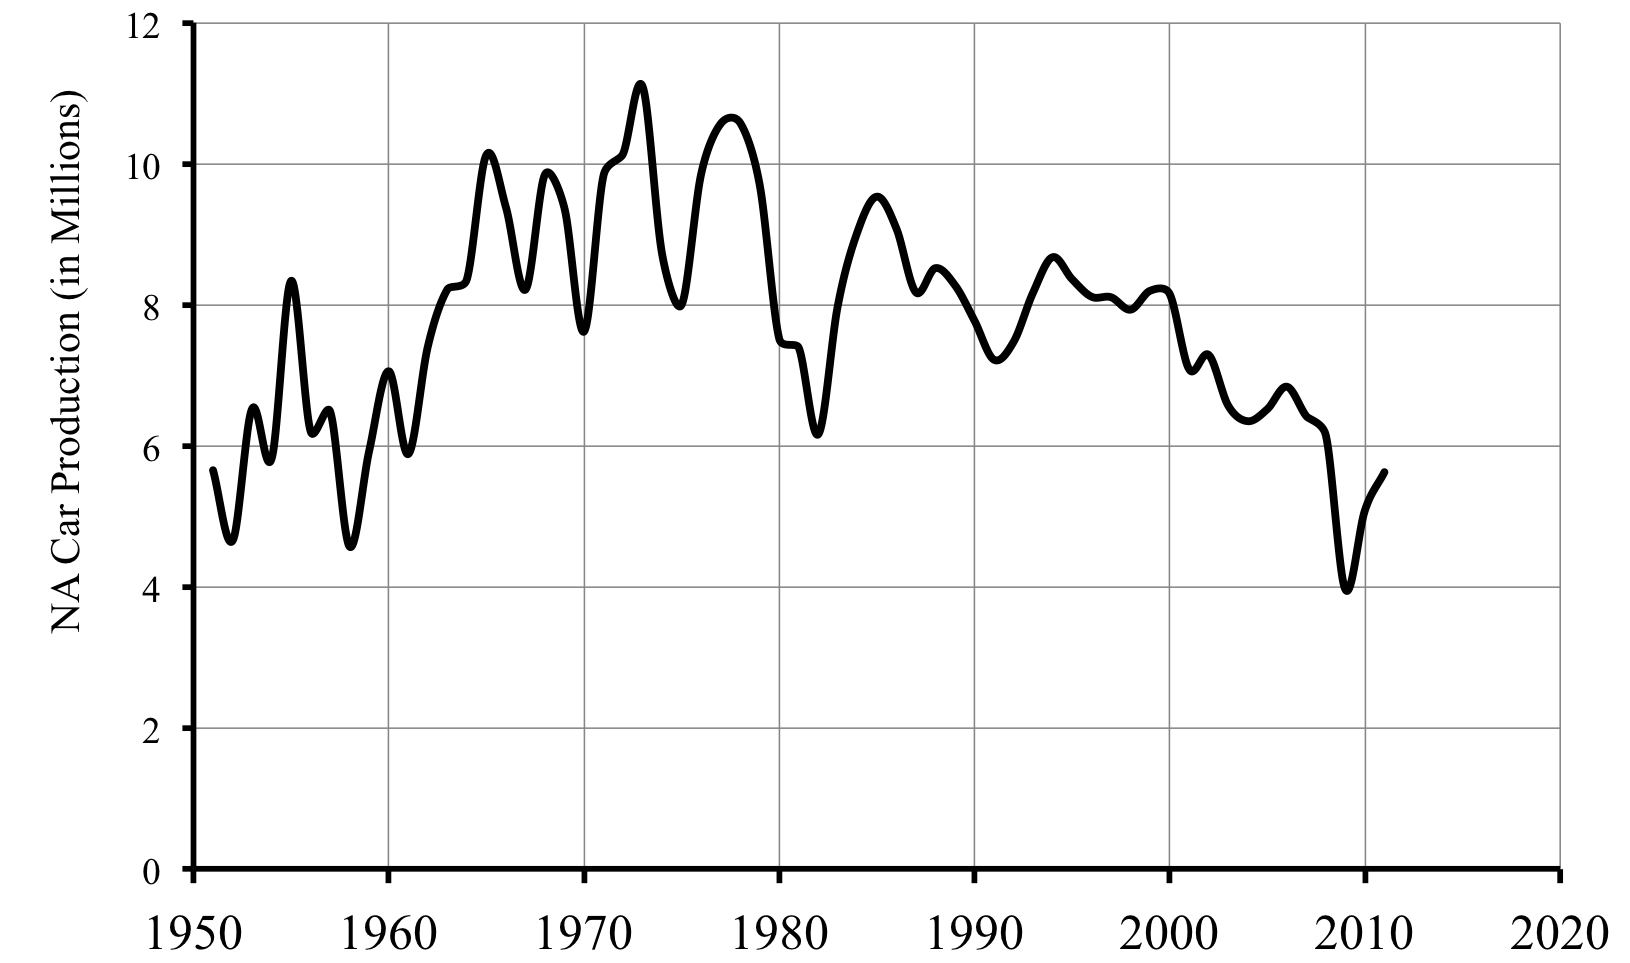
\includegraphics[width=\linewidth]{external/CarProduction.png}
\end{image}%
\begin{enumerate}[label=(\alph*),ref=\alph*]%
\item{}Identify the variables, including units and dependence.%
\par\rule{\workspacestrutwidth}{1.75in}%
\item{}\emph{The problem continues \textellipsis{}}%
\par
Approximately when did North American car production first pass 9 million\slash{}year? Indicate the corresponding point on the graph.%
\par\rule{\workspacestrutwidth}{0.75in}%
\item{}In which year were the most cars produced? Again, also indicate the point.%
\par\rule{\workspacestrutwidth}{0.75in}%
\item{}Best as you can tell from your graph, what might be a reasonable estimate of North American car production in 2015? Just guess to the nearest million\slash{}year.%
\par\rule{\workspacestrutwidth}{0.75in}%
\item{}Calculate the rate of change from 1958 when production was 4.57 million cars\slash{}year to 1971 when it was 9.83 cars million\slash{}year. What does that tell you about North American car production during 1958-1971?%
\par\rule{\workspacestrutwidth}{1.5in}%
\item{}Now calculate the rate of change of from 1984 when production was 9.03 million cars\slash{}year to 2006 when it was 6.84 million cars\slash{}year. What does that tell you about North American car production during 1984-2006?%
\end{enumerate}%
\end{divisionexercise}%
\clearpage
\begin{divisionexercise}{2}{}{}{stuffed-animals-PE6A}%
Sarah and Koal are bringing a large basket of stuffed animals to the crisis nursery as gifts for the children. They estimate it will cost \textdollar{}\(T\) for \(S\) stuffed animals where%
\begin{equation*}
T = 39.99 + 6.95S
\end{equation*}
%
\begin{enumerate}[label=(\alph*),ref=\alph*]%
\item{}Make a table showing the cost if Sarah and Koal include 10, 20, or 40 stuffed animals.%
\par\rule{\workspacestrutwidth}{0.9in}%
\item{}Included in the cost is a new toy box for the animals. What does it cost?%
\par\rule{\workspacestrutwidth}{0.9in}%
\item{}What does the 6.95 represent and what are its units?%
\par\rule{\workspacestrutwidth}{0.9in}%
\item{}Draw a detailed graph, starting at 0.%
\begin{image}{0.05}{0.9}{0.05}{}%

\includegraphics[width=\linewidth]{external/GraphPaper.jpg}
\end{image}%
\par\rule{\workspacestrutwidth}{0in}%
\item{}\emph{The problem continues \textellipsis{}}%
\par
If Sarah and Koal spent \textdollar{}262.39, how many stuffed animals were in the toy box they gave to the crisis nursery? Show how to set up and solve an equation to answer the question.%
\par\rule{\workspacestrutwidth}{3.5in}%
\item{}Solve the inequality%
\begin{equation*}
200 \le 39.99 + 6.95S \le 300
\end{equation*}
What does the answer mean in terms of the story?%
\par\rule{\workspacestrutwidth}{0.9in}%
\end{enumerate}%
\end{divisionexercise}%
\clearpage
\begin{divisionexercise}{3}{}{}{lbd-PE6A}%
My favorite little black dress is machine washable. Unfortunately each time I wash it the color fades a little. The intensity of black color remaining, \(B\), is a function of the number of times I have washed the dress, \(W\), according to the equation%
\begin{equation*}
B=100 \ast 0.985^W
\end{equation*}
%
\begin{enumerate}[label=(\alph*),ref=\alph*]%
\item{}It will still look new as long as the intensity stays above 90\%. Set up and solve an equation to figure out how many times I can wash the dress and keep it looking new. Then check some other way.%
\par\rule{\workspacestrutwidth}{1.2in}%
\item{}By the time only 75\% of the color remains, the dress will look too faded to wear formally. How many washes before then? Find the answer to the nearest number of washes by any method you prefer.%
\par\rule{\workspacestrutwidth}{1.2in}%
\item{}Draw a graph showing how the color of my favorite little black dress fades.%
\begin{image}{0.05}{0.9}{0.05}{}%

\includegraphics[width=\linewidth]{external/GraphPaper.jpg}
\end{image}%
\par\rule{\workspacestrutwidth}{0in}%
\end{enumerate}%
\end{divisionexercise}%
\clearpage
\begin{divisionexercise}{4}{}{}{gym-machines-PE6A}%
Brock is working as the equipment manager at a local gym. They need to replace several weight machines. One option will cost \textdollar{}475 per month to rent the machines plus a delivery\slash{}removal fee of \textdollar{}300. The other option is to buy the machines for \textdollar{}23,600 and pay \textdollar{}92\slash{}month for a service contract.%
\begin{enumerate}[label=(\alph*),ref=\alph*]%
\item{}Name the variables and write an equation for each option.%
\par\rule{\workspacestrutwidth}{2in}%
\item{}What should Brock recommend if they plan to have the machines for 3 years?%
\par\rule{\workspacestrutwidth}{1in}%
\item{}Set up and solve a system of equations to determine when the options cost the same.%
\par\rule{\workspacestrutwidth}{3in}%
\item{}What does the answer tell Brock?%
\end{enumerate}%
\end{divisionexercise}%
\clearpage
\begin{divisionexercise}{5}{}{}{business-sales-PE6A}%
Dwight's company was doing great business in 2000, but a few years later sales began to drop, and have only gotten worse. Their sales \textdollar{}\(S\) in millions \(T\) years from 2000 is given by the following equation%
\begin{equation*}
S = 78.1+5.75T-0.7T^2
\end{equation*}
%
 \begin{image}{0}{1}{0}{}%
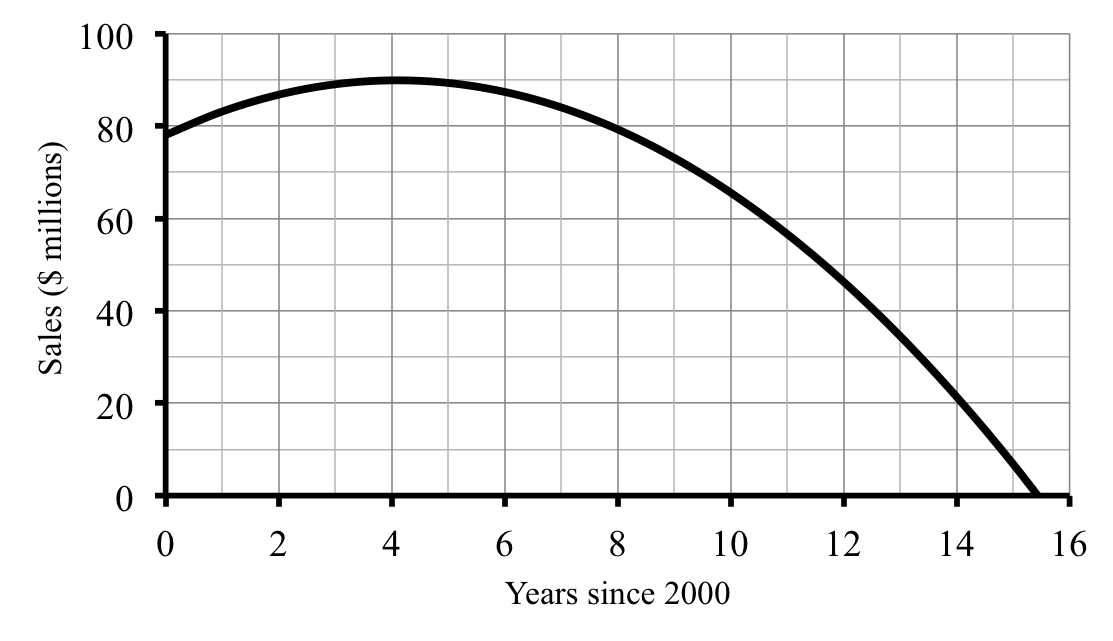
\includegraphics[width=\linewidth]{external/salesquad.png}
\end{image}%
\begin{enumerate}[label=(\alph*),ref=\alph*]%
\item{}According to this equation, what were the company's sales in 2000, 2004, 2009? \emph{You may confirm your answers with the graph, but use the equation to calculate.}%
\par\rule{\workspacestrutwidth}{1in}%
\item{}The company decided to declare bankruptcy when sales fell below \textdollar{}10 million. In what year was that? Find the answer to the nearest year, showing work to justify your answer. Also, indicate the point on the graph where you can check. \emph{You may use successive approximations or the appropriate formula.}%
\end{enumerate}%
\end{divisionexercise}%
\clearpage
\begin{divisionexercise}{6}{}{}{infant-weight-PE6A}%
Infants are regularly checked to make sure they are growing accordingly. The World Health Organization publishes growth charts to evaluate infant weight \(W\) in kilograms at a given age \(A\) in months since birth (for up to three years). An equation that describes an average infant boy is the following:%
\begin{equation*}
W=15-11.5\ast0.932^A
\end{equation*}
%
\begin{enumerate}[label=(\alph*),ref=\alph*]%
\item{}According to this equation, what is the average infant boy weight at birth, 4 months, a year, and 2 years?%
\par\rule{\workspacestrutwidth}{3in}%
\item{}Convert your answer for 4 months to pounds and ounces using%
\begin{equation*}
1 \text{ kilogram } \approx 2.2 \text{ pounds} \quad \text{ and } \quad 1 \text{ pound } = 16 \text{ ounces}
\end{equation*}
\emph{Hint: first convert to pounds. Then convert just the decimal part to ounces.}%
\end{enumerate}%
\end{divisionexercise}%
\clearpage
\begin{divisionexercise}{7}{}{}{fudge-square-PE6A}%
Gail calculated that number of pieces of fudge \(F\) she can cut from a square that is \(D\) inches on each edge is given by the formula%
\begin{equation*}
F=1.5625\, D^2
\end{equation*}
%
\begin{enumerate}[label=(\alph*),ref=\alph*]%
\item{}Make a table showing the number of pieces of fudge from a square with edge: 5 inches, 10 inches, and 2 feet. Include the value for a 0 inch square too.%
\par\rule{\workspacestrutwidth}{0.75in}%
\item{}Draw a graph showing how the number of pieces of fudge depends on the length of the edge of the square.%
\begin{image}{0.05}{0.9}{0.05}{}%

\includegraphics[width=\linewidth]{external/GraphPaper.jpg}
\end{image}%
\par\rule{\workspacestrutwidth}{0in}%
\item{}According to your graph, \emph{approximately} what size square should Gail make if she wants 200 pieces of fudge?%
\par\rule{\workspacestrutwidth}{0.75in}%
\item{}Now set up and solve an equation to find the answer to the nearest one decimal place.%
\par\rule{\workspacestrutwidth}{0in}%
\end{enumerate}%
\end{divisionexercise}%
\clearpage
\begin{divisionexercise}{8}{}{}{texas-population-PE6A}%
\begin{aside}{Aside}{}{texas-population-PE6A-1-1}%
Source: United States Census Bureau%
\end{aside}
 In 2000 there were an estimated 20,851,820 Texans. The population of Texas has grown around 1.89\% per year since then.%
\begin{enumerate}[label=(\alph*),ref=\alph*]%
\item{}Name the variables and write an equation relating them.%
\par\rule{\workspacestrutwidth}{3.5in}%
\item{}According to your equation, what was the population of Texas in 2010?%
\par\rule{\workspacestrutwidth}{2in}%
\item{}The U.S. Census Bureau counted 25,145,561 Texans in 2010. Does that mean the actual growth rate was slightly more or slightly less than 1.89\%? Explain.%
\end{enumerate}%
\end{divisionexercise}%
\clearpage
\begin{divisionexercise}{9}{}{}{curl-weight-PE6A}%
Ericson has been lifting weight for the past 12 weeks. He has increased his curl weight by about 1.5 pounds per week and is up to 30 pounds.%
\begin{enumerate}[label=(\alph*),ref=\alph*]%
\item{}What weight could Ericson curl 12 weeks ago?%
\par\rule{\workspacestrutwidth}{2.5in}%
\item{}Name the variables and write a linear equation relating them.%
\par\rule{\workspacestrutwidth}{2.5in}%
\item{}At this rate when will Ericson be able to curl his goal of at least 45 pounds? Set up and solve an inequality.%
\par\rule{\workspacestrutwidth}{0in}%
\end{enumerate}%
\end{divisionexercise}%
\clearpage
\begin{divisionexercise}{10}{}{}{calories-PE6A}%
\begin{aside}{Aside}{}{calories-PE6A-1-1}%
Source: United States Department of Agriculture%
\end{aside}
 In the United States in 1970, the average person ate 2,169 calories per day. By 2008 that number had increased to 2,674 calories per day. Let \(C\) be the amount a typical person eats (in calories per day) and \(T\) the number of years since 1970. Compare what the linear and exponential models project for the years 2015 and 2030. Include both equations and a graph showing both functions on the same axes.%
 \begin{image}{0.05}{0.9}{0.05}{}%

\includegraphics[width=\linewidth]{external/GraphPaper.jpg}
\end{image}%
\end{divisionexercise}%
\end{exercises-subsection-numberless}
\end{sectionptx}
%
%
\typeout{************************************************}
\typeout{Section A.2 Practice Final Exam 2}
\typeout{************************************************}
%
\begin{sectionptx}{Section}{Practice Final Exam 2}{}{Practice Final Exam 2}{}{}{sec-pfe2}
%
%
\typeout{************************************************}
\typeout{Exercises A.2 }
\typeout{************************************************}
%
\begin{exercises-subsection-numberless}{Exercises}{}{}{}{}{}{ws-PE6B}
\begin{introduction}{}%
\emph{Try taking this version of the practice exam under testing conditions: no book, no notes, no classmate's help, no electronics (computer, cell phone, television). Give yourself two hours to work and wait until you have tried your best on all of the problems before checking any answers.}%
\end{introduction}%
\begin{divisionexercise}{1}{}{}{coffee-temp-PE6B}%
I love coffee. But not when it gets cold. The graph shows how my cup of coffee cools.%
 \begin{image}{0}{1}{0}{}%
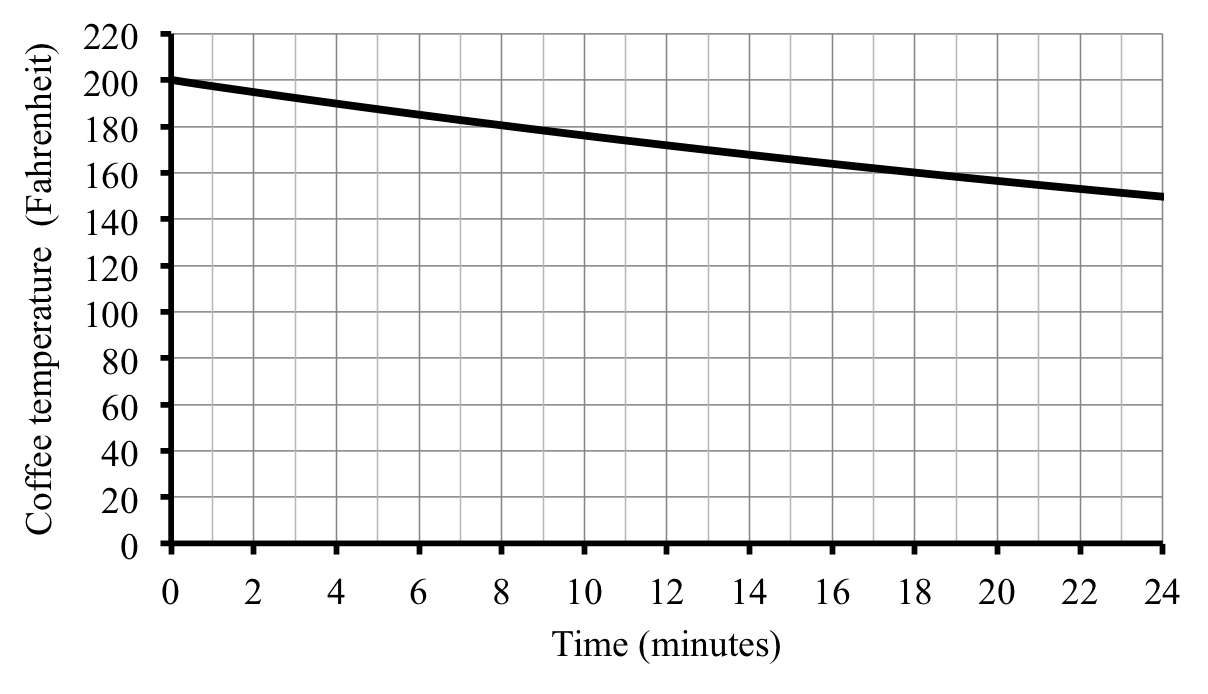
\includegraphics[width=\linewidth]{external/coffeecooling.png}
\end{image}%
\begin{enumerate}[label=(\alph*),ref=\alph*]%
\item{}Identify the variables, including units and dependence.%
\par\rule{\workspacestrutwidth}{0.5in}%
\item{}Answer each question and indicate the point on the graph you use.%
\begin{enumerate}[label=\roman*.,ref=\theenumi.\roman*]%
\item{}How hot is my coffee right after I pour it (before it starts cooling)?%
\par\rule{\workspacestrutwidth}{0.25in}%
\item{}I simply will not drink my coffee once it is cooler than 150\textdegree{}F. How long does it take for my coffee to cool off that much?%
\par\rule{\workspacestrutwidth}{0.25in}%
\item{}I prefer to drink my coffee between 160\textdegree{}F and 180\textdegree{}F. What is the corresponding time period during which I should drink my coffee?%
\par\rule{\workspacestrutwidth}{0.25in}%
\end{enumerate}%
\end{enumerate}%
\end{divisionexercise}%
\clearpage
\begin{divisionexercise}{2}{}{}{traffic-linear-PE6B}%
Jolene is driving up to Duluth to visit her aunt. Unfortunately it is snowing so traffic is going slowly. Her distance \(D\) miles to Duluth is described by the equation%
\begin{equation*}
D=100-45T
\end{equation*}
where \(T\) is the time in hours since 12:00 noon when Jolene started driving.%
\begin{enumerate}[label=(\alph*),ref=\alph*]%
\item{}Identify the intercept, including units, and explain what it means in the story.%
\par\rule{\workspacestrutwidth}{2in}%
\item{}Identify the slope, including units, and explain what it means in the story.%
\par\rule{\workspacestrutwidth}{2in}%
\item{}Jolene plans to call her aunt once she is under 20 miles from Duluth. When will that be? Show how to set up and solve an inequality to answer the question. Find the exact time, to the nearest minute.%
\par\rule{\workspacestrutwidth}{2in}%
\end{enumerate}%
\end{divisionexercise}%
\clearpage
\begin{divisionexercise}{3}{}{}{squirrels-PE6B}%
There sure are a lot of squirrels in my neighborhood. The equation%
\begin{equation*}
S = 4,000\ast 1.12^T
\end{equation*}
estimates the number of squirrels (\(S\)) where \(T\) is the time in years since 2005.%
\begin{enumerate}[label=(\alph*),ref=\alph*]%
\item{}Make a table showing the number of squirrels in 2005, 2008, 2013, and 2017.%
\par\rule{\workspacestrutwidth}{2.5in}%
\item{}Draw a graph showing how the squirrel population grew.%
\begin{image}{0.05}{0.9}{0.05}{}%

\includegraphics[width=\linewidth]{external/GraphPaper.jpg}
\end{image}%
\par\rule{\workspacestrutwidth}{1in}%
\item{}\emph{The problem continues \textellipsis{}}%
\par
\emph{Approximately} when will the population pass 10,000 squirrels? Guess from the graph. Then refine your answer using successive approximation.%
\par\rule{\workspacestrutwidth}{2in}%
\item{}Show how to solve the equation to determine \emph{exactly} when there will be 10,000 squirrels.%
\par\rule{\workspacestrutwidth}{2in}%
\item{}There were 10,000 squirrels in 2011, so our equation is a bit off. Assuming there were still 4,000 squirrels in 2005, revise the equation. \emph{Hint: find the new growth factor.}%
\par\rule{\workspacestrutwidth}{2in}%
\end{enumerate}%
\end{divisionexercise}%
\clearpage
\begin{divisionexercise}{4}{}{}{fudge-calories-PE6B}%
Gail calculated that the number of calories \(C\) in a cube of fudge depends on how large the cube is, say \(E\) inches long on each edge. A possible equation is%
\begin{equation*}
C = 90E^3
\end{equation*}
%
\begin{enumerate}[label=(\alph*),ref=\alph*]%
\item{}How many calories are in a cube of fudge that is 1 inch on each edge?%
\par\rule{\workspacestrutwidth}{1.5in}%
\item{}What size cube of fudge has 200 calories? Answer to the nearest tenth (that means to 1 decimal place), showing work to justify your answer.%
\par
\emph{You may use successive approximations or the appropriate formula.}%
\par\rule{\workspacestrutwidth}{3in}%
\item{}Convert your answer to millimeters (mm) using \(1 \text{ inch} \approx 2.54 \text{ cm and }1 \text{ cm} = 10 \text{ mm}\).%
 \par
\emph{Test-taking tip: No answer for part (b)? Write down a guess and convert that.}%
%
\end{enumerate}%
\end{divisionexercise}%
\clearpage
\begin{divisionexercise}{5}{}{}{ball-in-air-PE6B}%
The height \(H\) feet of a ball \(T\) seconds after it is thrown straight up in the air is given by the equation%
\begin{equation*}
H = 4+17T-16T^2
\end{equation*}
%
 \begin{image}{0}{1}{0}{}%
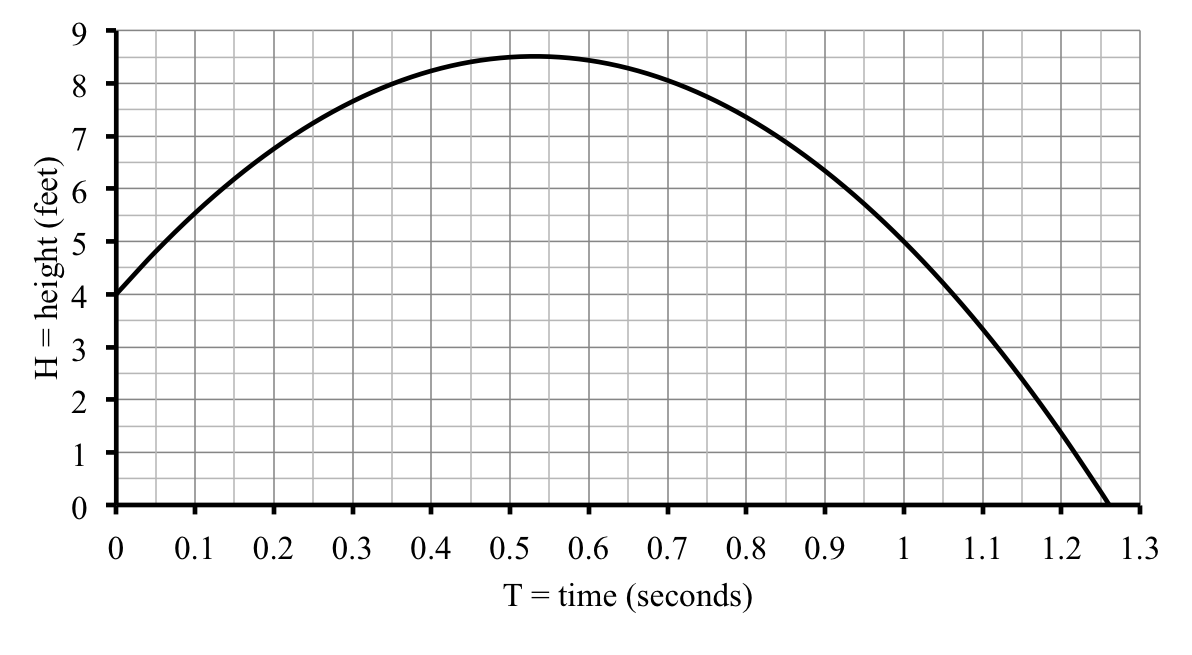
\includegraphics[width=\linewidth]{external/ballinair.png}
\end{image}%
\begin{enumerate}[label=(\alph*),ref=\alph*]%
\item{}According to the equation, how high up was the ball to start, after 0.5 seconds, and after 1 second? \emph{Use the equation to evaluate and check against the graph.}%
\par\rule{\workspacestrutwidth}{1.75in}%
\item{}Calculate the speed (rate of change) between 0.7 seconds and 0.8 seconds.%
\par\rule{\workspacestrutwidth}{2in}%
\item{}\emph{The problem continues \textellipsis{}}%
\par
Convert your answer from part (b) to mph. Use 1 mile = 5,280 feet.%
\par
\emph{Test-taking tip: No answer for part (b)? Write down a guess and convert that.}%
\par\rule{\workspacestrutwidth}{2in}%
\item{}When will the ball hit the ground? Find the answer to the nearest hundredth (that means to 2 decimal places), showing work to justify your answer.%
\par
\emph{You may use successive approximations or the appropriate formula.}%
\end{enumerate}%
\end{divisionexercise}%
\clearpage
\begin{divisionexercise}{6}{}{}{custom-jerseys-PE6B}%
A local sporting goods store does custom embroidered jerseys for \textdollar{}29 each plus \textdollar{}1.75 per letter. Or you can order the same jerseys online for \textdollar{}18 each plus \textdollar{}2.35 per letter, but it costs another \textdollar{}4.95 for shipping per jersey. If we write \(L\) for the number of letters on the jersey and \(T\) for the total cost (in \textdollar{}), then those equations are%
\begin{equation*}
\textbf{Local shop:} \quad T = 29 + 1.75L
\end{equation*}
%
\begin{equation*}
\textbf{Online:} \quad T = 22.95+2.35L
\end{equation*}
%
\begin{enumerate}[label=(\alph*),ref=\alph*]%
\item{}If a player named \terminology{Redeisheimer} (12 letters) wants a jersey, which option costs least?%
\par\rule{\workspacestrutwidth}{1in}%
\item{}Make a table showing the cost for players named: \terminology{Buls} (4 letters), \terminology{Schaaf} (6 letters), and \terminology{Johnston} (8 letters).%
\par\rule{\workspacestrutwidth}{1in}%
\item{}Set up and solve a system of equations to determine when the options cost the same.%
\par\rule{\workspacestrutwidth}{3in}%
\item{}Summarize your findings in words.%
\item{}\emph{The problem continues \textellipsis{}}%
\par
Graph both functions on the same set of axes. \emph{Don't forget 0 letters.}%
\begin{image}{0.05}{0.9}{0.05}{}%

\includegraphics[width=\linewidth]{external/GraphPaper.jpg}
\end{image}%
\item{}Indicate the point on your graph where you can check your solution to part (c). If it doesn't agree, check your work and\slash{}or your graph again.%
\end{enumerate}%
\end{divisionexercise}%
\clearpage
\begin{divisionexercise}{7}{}{}{empanadas-PE6B}%
For their holiday party at the office, Adriana had a tray of 200 empanadas delivered for \textdollar{}196. They were so good that she had a tray of 72 empanadas delivered to bring to her sister's house on Christmas Eve, which cost \textdollar{}78.24. Assume that the total cost is a linear function of the number of empanadas.%
 \par
\emph{Test-taking tip: Note sure about parts (b) and (c)? Try finding the equation first.}%
\begin{enumerate}[label=(\alph*),ref=\alph*]%
\item{}Name the variables, including units and dependence.%
\par\rule{\workspacestrutwidth}{1.5in}%
\item{}What does each empanada cost?%
\par\rule{\workspacestrutwidth}{1.5in}%
\item{}What is the delivery charge?%
\par\rule{\workspacestrutwidth}{1.5in}%
\item{}Write an equation for the function.%
\par\rule{\workspacestrutwidth}{0in}%
\end{enumerate}%
\end{divisionexercise}%
\clearpage
\begin{divisionexercise}{8}{}{}{light-rail-PE6B}%
Light rail fares are currently \textdollar{}3.00 per ride during rush hour. Two different plans of increasing fares are being debated: 15¢ per year or 4.5\% per year.%
\begin{enumerate}[label=(\alph*),ref=\alph*]%
\item{}Name the variables, including units and dependence.%
\par\rule{\workspacestrutwidth}{2.25in}%
\item{}Write an equation describing light rail fares over the next few years, assuming they increase 15¢ per year. What is this type of function called?%
\par\rule{\workspacestrutwidth}{2.25in}%
\item{}Write an equation describing light rail fares over the next few years, assuming they increase 4.5\% per year. What is this type of function called?%
\par\rule{\workspacestrutwidth}{2in}%
\item{}\emph{The problem continues \textellipsis{}}%
\par
Compare what each equation tells you light rail fares would be in 1 year, 5 years, and 20 years. List your answers in a table.%
\par\rule{\workspacestrutwidth}{2.8in}%
\item{}Graph both options on the same set of axes. \emph{Don't forget now.}%
\begin{image}{0.05}{0.9}{0.05}{}%

\includegraphics[width=\linewidth]{external/GraphPaper.jpg}
\end{image}%
\par\rule{\workspacestrutwidth}{0in}%
\end{enumerate}%
\end{divisionexercise}%
\end{exercises-subsection-numberless}
\end{sectionptx}
\end{appendixptx}
%
%
\typeout{************************************************}
\typeout{Appendix B Templates and Formulas}
\typeout{************************************************}
%
\begin{appendixptx}{Appendix}{Templates and Formulas}{}{Templates and Formulas}{}{}{app-templates-formulas}
\renewcommand*{\appendixname}{Appendix}
\begin{introduction}{}%
Templates are used to write equations from given or calculated information, to read constants from the equations, or simply to identify the type of equation in order to use type-specific formulas or information.%
\par
Formulas are used for many purposes, including finding constants or solving specific types of equations. Various disciplines, such as finance, have specific formulas to evaluate quantities.%
\end{introduction}%
%
%
\typeout{************************************************}
\typeout{Section B.1 Templates}
\typeout{************************************************}
%
\begin{sectionptx}{Section}{Templates}{}{Templates}{}{}{sec-templates}
\begin{assemblage}{Assemblage}{Linear Equation Template}{sec-templates-2}%
%
\begin{equation*}
\text{dep} = \text{start} + \text{slope} \ast \text{indep}
\end{equation*}
%
\end{assemblage}
\begin{assemblage}{Assemblage}{Power Equation Template}{sec-templates-3}%
%
\begin{equation*}
\text{dep} = k \ast \text{indep}^{n}
\end{equation*}
%
\end{assemblage}
\begin{assemblage}{Assemblage}{Quadratic Equation Template}{sec-templates-4}%
%
\begin{equation*}
\text{dep} = a \ast \text{indep}^2 + b \ast\text{indep} + c
\end{equation*}
%
\end{assemblage}
\begin{assemblage}{Assemblage}{Exponential Equation Template}{sec-templates-5}%
%
\begin{equation*}
\text{dep} = \text{start} \ast \text{growth factor} ^ {\text{indep}}
\end{equation*}
%
\end{assemblage}
\end{sectionptx}
%
%
\typeout{************************************************}
\typeout{Section B.2 Formulas used to find constants}
\typeout{************************************************}
%
\begin{sectionptx}{Section}{Formulas used to find constants}{}{Formulas used to find constants}{}{}{sec-formula-constants}
\begin{assemblage}{Assemblage}{Rate of Change Formula}{sec-formula-constants-2}%
%
\begin{equation*}
\text{rate of change } = \frac{\text{change dep}}{\text{change indep}} = \frac{\text{1st dep - 2nd dep}}{\text{1st indep - 2nd indep}}
\end{equation*}
%
\end{assemblage}
\begin{assemblage}{Assemblage}{Intercept (of Linear) Formula}{sec-formula-constants-3}%
If we know a value of indep and the corresponding value of dep, then we can find the intercept:%
\begin{equation*}
\text{intercept} = \text{dep} - \text{slope}\ast\text{indep}
\end{equation*}
%
\end{assemblage}
\begin{assemblage}{Assemblage}{Percent Change Formula}{sec-formula-constants-4}%
%
\begin{itemize}[label=\textbullet]
\item{}If a quantity changes by a percentage corresponding to growth rate \(r\), then the growth factor is%
\begin{equation*}
\displaystyle g=1+r
\end{equation*}
%
\item{}If the growth factor is \(g\), then the growth rate is%
\begin{equation*}
r = g-1
\end{equation*}
%
\end{itemize}
%
\end{assemblage}
\begin{assemblage}{Assemblage}{Growth Factor Formula}{sec-formula-constants-5}%
If a quantity is growing (or decaying) exponentially, then the growth (or decay) factor is%
\begin{equation*}
\displaystyle g = \sqrt[t]{\frac{a}{s}}
\end{equation*}
where \(s\) is the starting amount and \(a\) is the amount after \(t\) time periods.%
\end{assemblage}
\end{sectionptx}
%
%
\typeout{************************************************}
\typeout{Section B.3 Formulas used to solve specific types of equations}
\typeout{************************************************}
%
\begin{sectionptx}{Section}{Formulas used to solve specific types of equations}{}{Formulas used to solve specific types of equations}{}{}{sec-formula-solve}
\begin{assemblage}{Assemblage}{Root Formula}{sec-formula-solve-2}%
The equation \(C^n=v\) has solution%
\begin{equation*}
C= \sqrt[n]{v}
\end{equation*}
%
\end{assemblage}
\begin{assemblage}{Assemblage}{Log-Divides Formula}{sec-formula-solve-3}%
The equation \(g^Y = v\) has solution%
\begin{equation*}
Y = \frac{\log (v)}{\log(g)}
\end{equation*}
%
\end{assemblage}
\begin{assemblage}{Assemblage}{Quadratic Formula}{sec-formula-solve-4}%
The equation \(aT^2+bT+c=0\) has solutions%
\begin{equation*}
T = \frac{-b}{2a} \pm \frac{\sqrt{b^2-4ac}}{2a}
\end{equation*}
%
\end{assemblage}
\end{sectionptx}
%
%
\typeout{************************************************}
\typeout{Section B.4 Formulas from finance}
\typeout{************************************************}
%
\begin{sectionptx}{Section}{Formulas from finance}{}{Formulas from finance}{}{}{sec-formula-finance}
\begin{assemblage}{Assemblage}{Compound Interest Formula}{sec-formula-finance-2}%
%
\begin{equation*}
a = p \left( 1 + \frac{r}{12}\right) ^{12y}
\end{equation*}
%
\begin{itemize}[label=\textbullet]
\item{}\(a\) = account balance (\textdollar{})%
\item{}\(y\) = time invested (years)%
\item{}\(p\) = initial deposit or ``principal''%
\item{}\(r\) = interest rate compounded monthly (as a decimal)%
\end{itemize}
%
\end{assemblage}
\begin{assemblage}{Assemblage}{Equivalent APR Formula}{sec-formula-finance-3}%
%
\begin{equation*}
\text{APR} = \left(1+\frac{r}{12}\right)^{12}-1
\end{equation*}
where \(r\) = interest rate compounded monthly (as a decimal)%
\end{assemblage}
\begin{assemblage}{Assemblage}{Future Value Annuity Formula}{sec-formula-finance-4}%
%
\begin{equation*}
a = p \ast \frac{\left( 1 + \frac{r}{12}\right) ^{12y}-1}{\frac{r}{12}}
\end{equation*}
%
\begin{itemize}[label=\textbullet]
\item{}\(a\) = account balance (\textdollar{})%
\item{}\(y\) = time invested (years)%
\item{}\(p\) = regular (monthly) deposits (\textdollar{})%
\item{}\(r\) = interest rate compounded monthly (as a decimal)%
\end{itemize}
%
\end{assemblage}
\begin{assemblage}{Assemblage}{Loan Payment Formula}{sec-formula-finance-5}%
%
\begin{equation*}
p = \frac{a  \ast \frac{r}{12}}{1-\left( 1 + \frac{r}{12}\right) ^{-12y}}
\end{equation*}
%
\begin{itemize}[label=\textbullet]
\item{}\(a\) = loan amount (\textdollar{})%
\item{}\(y\) = time invested (years)%
\item{}\(p\) = regular (monthly) payment (\textdollar{})%
\item{}\(r\) = interest rate compounded monthly (as a decimal)%
\end{itemize}
%
\end{assemblage}
\end{sectionptx}
\end{appendixptx}
%
\backmatter%
%
\clearpage\phantomsection%
\addcontentsline{toc}{part}{Back Matter}%
\end{document}
